\documentclass[11pt,a4paper]{amsart}
\usepackage[a3paper,landscape,margin=20mm]{geometry}
\usepackage{amsmath,amssymb,amsthm,graphicx,xcolor,mathrsfs}
\usepackage[no-math]{fontspec}
\setmainfont{lmroman10-regular.otf}[BoldFont=lmroman10-bold.otf,ItalicFont=lmroman10-italic.otf,BoldItalicFont=lmroman10-bolditalic.otf,SmallCapsFont=lmromancaps10-regular.otf]
\usepackage[numbers]{natbib}
\usepackage{hyperref}
\usepackage[all,cmtip,2cell]{xy}
\usepackage{booktabs,subcaption,stmaryrd,tikz,url,multirow,multicol,rotating,listings,bussproofs,enumitem,fancyvrb}
\usepackage[normalem]{ulem}
\usetikzlibrary{shapes,calc}
\renewcommand\simeq\cong
\definecolor{light-gray}{gray}{0.85}
\newcommand\coll[1]{{\colorbox{light-gray}{$#1$}}}
\AtBeginDocument{\def\shorttitle{Nominal recursors as epi-recursors}}

%\usepackage{amssymb}

\newenvironment{myitem}[1][]
{\itemize[leftmargin=5.0ex,topsep=0.3ex,itemsep=1pt, #1]}
{\enditemize}
\newenvironment{myyitem}[1][]
{\itemize[leftmargin=4.0ex,topsep=0.3ex,itemsep=1pt, #1]}
{\enditemize}
\newenvironment{myyyitem}[1][]
{\itemize[leftmargin=3.7ex,topsep=0.3ex,itemsep=1pt, #1]}
{\enditemize}
\newenvironment{mmyitem}[1][]
{\itemize[leftmargin=2.15ex,topsep=0.3ex,itemsep=1pt, #1]}
{\enditemize}
\newenvironment{mmmyitem}[1][]
{\itemize[leftmargin=3.2ex,topsep=0.3ex,itemsep=1pt, #1]}
{\enditemize}
\newenvironment{mmmmyitem}[1][]
{\itemize[leftmargin=0.5ex,topsep=0.3ex,itemsep=1pt, #1]}
{\enditemize}
\newenvironment{myitemm}[1][]
{\itemize[leftmargin=6ex,topsep=1ex,itemsep=1pt, #1]}
{\enditemize}
\newenvironment{myitemmm}[1][]
{\itemize[leftmargin=22ex,topsep=1ex,itemsep=1pt, #1]}
{\enditemize}
\newenvironment{myitemmmm}[1][]
{\itemize[leftmargin=20ex,topsep=1ex,itemsep=1pt, #1]}
{\enditemize}
\newenvironment{myenum}[1][]
{\enumerate[leftmargin=5ex,topsep=1ex,itemsep=1pt, #1]}
{\endenumerate}

\setcounter{secnumdepth}{4}



%\newcommand\mystyle[1]{\textsf{(#1)}}
\newcommand\mystyle[1]{{\small \textsf{#1}}}

\newcommand\FrVr{\mystyle{FrVr}}
\newcommand\FrVrT{\mystyle{FrVr}$_2$}
\newcommand\FrAp{\mystyle{FrAp}}
\newcommand\FrLm{\mystyle{FrLm}}
\newcommand\FvVr{\mystyle{FvVr}}
\newcommand\FvAp{\mystyle{FvAp}}
\newcommand\FvLm{\mystyle{FvLm}}

\newcommand\co[1]{#1$_\infty$}

\newcommand\IFrVr{\co{\FrVr}}
\newcommand\IIFrVr{\FrVr$_\infty'$}
\newcommand\VrInv{\mystyle{VrInv}}
\newcommand\IFrAp{\co{\FrAp}}
\newcommand\IFrLm{\co{\FrLm}}
\newcommand\IFvVr{\co{\FvVr}}
\newcommand\IFvAp{\co{\FvAp}}
\newcommand\IFvLm{\co{\FvLm}}

\newcommand\SwVr{\mystyle{SwVr}}
\newcommand\SwAp{\mystyle{SwAp}}
\newcommand\SwLm{\mystyle{SwLm}}
\newcommand\ISwVr{\co{\SwVr}}
\newcommand\ISwAp{\co{\SwAp}}
\newcommand\ISwLm{\co{\SwLm}}


\newcommand\SwId{\mystyle{SwId}}
\newcommand\SwCp{\mystyle{SwCp}}
\newcommand\SwIv{\mystyle{SwIv}}
\newcommand\SwFr{\mystyle{SwFr}}
\newcommand\FrSw{\mystyle{FrSw}}
\newcommand\SwFv{\mystyle{SwFv}}
\newcommand\FvSw{\mystyle{FvSw}}

\newcommand\ISwId\SwId %{\co{\SwId}}
\newcommand\ISwCp\SwCp % {\co{\SwCp}}
\newcommand\ISwIv\SwIv %{\co{\SwIv}}
\newcommand\ISwFr\SwFr % {\co{\SwFr}}
\newcommand\IFrSw\FrSw %{\co{\FrSw}}
\newcommand\ISwFv\SwFv %{\co{\SwFv}}
\newcommand\IFvSw\FvSw %{\co{\FvSw}}

\newcommand\RnFr{\mystyle{RnFr}}
\newcommand\FrRn{\mystyle{FrRn}}
\newcommand\IRnFr\RnFr %{\co{\RnFr}}
\newcommand\IFrRn\FrRn %{\co{\FrRn}}

\newcommand\FrRnT{\mystyle{FrRn$_2$}}
\newcommand\IFrRnT\FrRnT

\newcommand\SbFr{\mystyle{SbFr}}
\newcommand\FrSb{\mystyle{FrSb}}
\newcommand\ISbFr\SbFr %{\co{\SbFr}}
\newcommand\IFrSb\FrSb %{\co{\FrSb}}


\newcommand\SwCg{\mystyle{SwCg}}
\newcommand\ISwCg{\co{\SwCg}}
\newcommand\SwCn{\mystyle{SwCn}}
%\newcommand\SwRn{\mystyle{SwRn}}
\newcommand\SwBvr{\mystyle{SwBvr}}
\newcommand\ISwBvr{\co{\SwBvr}}
\newcommand\ISwBvrT{\mystyle{SwBvr}$_{\infty,2}$}

\newcommand\PmVr{\mystyle{PmVr}}
\newcommand\PmAp{\mystyle{PmAp}}
\newcommand\PmLm{\mystyle{PmLm}}
\newcommand\IPmVr{\co{\PmVr}}
\newcommand\IPmAp{\co{\PmAp}}
\newcommand\IPmLm{\co{\PmLm}}

\newcommand\PmId{\mystyle{PmId}}
\newcommand\PmCp{\mystyle{PmCp}}
\newcommand\PmFv{\mystyle{PmFv}}
\newcommand\FvPm{\mystyle{FvPm}}

\newcommand\IPmId\PmId %{\co{\PmId}}
\newcommand\IPmCp\PmCp % {\co{\PmCp}}
\newcommand\IPmFv\PmFv %{\co{\PmFv}}
\newcommand\IFvPm\FvPm %{\co{\FvPm}}

\newcommand\PmBvr{\mystyle{PmBvr}}
\newcommand\IPmBvr{\co{\PmBvr}}
\newcommand\IIPmBvr{\PmBvr$_\infty'$}

\newcommand\SbVr{\mystyle{SbVr}}
\newcommand\SbAp{\mystyle{SbAp}}
\newcommand\SbLm{\mystyle{SbLm}}
\newcommand\ISbVr{\co{\SbVr}}
\newcommand\ISbAp{\co{\SbAp}}
\newcommand\ISbLm{\co{\SbLm}}


\newcommand\SbCn{\mystyle{SbCn}}
\newcommand\ISbCn\SbCn %{\co{\SbCn}}
%\newcommand\SbRn{\mystyle{SbRn}}
%\newcommand\ISbRn{\co{\SbRn}}

\newcommand\SbCg{\mystyle{SbCg}}
\newcommand\ISbCg{\co{\SbCg}}
\newcommand\SbBvr{\mystyle{SbBvr}}
\newcommand\ISbBvr{\co{\SbBvr}}
\newcommand\IISbBvr{\SbBvr$_\infty'$}


\newcommand\RnBvr{\mystyle{RnBvr}}
\newcommand\IRnBvr{\co{\RnBvr}}

\newcommand\RnBvrT{\RnBvr$_2$}


\newcommand\IIRnBvr{\RnBvr$_\infty'$}

\newcommand\RnVr{\mystyle{RnVr}}
\newcommand\RnAp{\mystyle{RnAp}}
\newcommand\RnLmO{\mystyle{RnLm$_1$}}
\newcommand\RnLmT{\mystyle{RnLm$_2$}}

\newcommand\IRnVr{\co{\RnVr}}
\newcommand\IRnAp{\co{\RnAp}}
\newcommand\IRnLmO{\mystyle{RnLm}$_{1,\infty}$}
\newcommand\IRnLmT{\mystyle{RnLm}$_{2,\infty}$}


\newcommand\RnCg{\mystyle{RnCg}}
\newcommand\IRnCg{\co{\RnCg}}

\newcommand\RnId{\mystyle{RnId}}
\newcommand\RnIm{\mystyle{RnIm}}
\newcommand\RnCh{\mystyle{RnCh}}
\newcommand\RnCm{\mystyle{RnCm}}
\newcommand\RnChFr{\mystyle{RnChFr}}
\newcommand\SbChFr{\mystyle{SbChFr}}

\newcommand\IRnId\RnId %{\co{\RnId}}
\newcommand\IRnIm\RnIm %{\co{\RnIm}}
\newcommand\IRnCh\RnCh %{\co{\RnCh}}
\newcommand\IRnCm\RnCm %{\co{\RnCm}}
\newcommand\IRnChFr\RnChFr %{\co{\RnChFr}}
\newcommand\ISbChFr\SbChFr %{\co{\SbChFr}}

\newcommand\SbId{\mystyle{SbId}}
\newcommand\SbIm{\mystyle{SbIm}}
\newcommand\SbCh{\mystyle{SbCh}}
\newcommand\SbCm{\mystyle{SbCm}}

\newcommand\ISbId\SbId %{\co{\SbId}}
\newcommand\ISbIm\SbIm %{\co{\SbIm}}
\newcommand\ISbCh\SbCh %{\co{\SbCh}}
\newcommand\ISbCm\SbCm %{\co{\SbCm}}

\newcommand\FSupFv{\mystyle{FSupFv}}
\newcommand\FSupFr{\mystyle{FSupFr}}
\newcommand\FvDPm{\mystyle{FvDPm}}
\newcommand\FvDSw{\mystyle{FvDSw}}
\newcommand\FrDSw{\mystyle{FrDSw}}
\newcommand\FrDRn{\mystyle{FrDRn}}
\newcommand\FCB{\mystyle{FCB}}

%\newcommand\IFSup{\co{\FSup}}
\newcommand\IFvDPm{\co{\FvDPm}}
\newcommand\IFvDSw{\co{\FvDSw}}
\newcommand\IFrDSw{\co{\FrDSw}}
\newcommand\IFrDRn{\co{\FrDRn}}
%\newcommand\IFCB{\mystyle{FCB}$_\infty$}
\newcommand\IFSupFv{\co{\FSupFv}}
\newcommand\IFSupFr{\co{\FSupFr}}


%Theorems and such
%\theoremstyle{definition}
%\makeatletter
%\def\thm@space@setup{%
%	\thm@preskip=50pt
%	\thm@postskip=\thm@preskip % or whatever, if you don't want them to be equal
%}
%\makeatother

\newtheorem{mylemma}{Lemma}
%\newtheorem{assm}[mylemma]{Assumption} 
\newtheorem{prop}[mylemma]{Prop}
\newtheorem{thm}[mylemma]{Thm}
\newtheorem{defi}[mylemma]{Def}
% \newtheorem{cconj}[mylemma]{Conjecture}
% %\newtheorem{theorem}{Theorem}
% \newtheorem{prop}[theorem]{Prop\hbox{.}}
\newtheorem{notation}[mylemma]{Notation}
% \newtheorem{assumption}[mylemma]{Assumption}
\newtheorem{rremark}[mylemma]{Remark}
% %\newtheorem{remark}{Remark}
% %\newtheorem{pproposition}{Prop.$^*$} %%% what is that? -- Jasmin
\newtheorem{coro}[mylemma]{Corollary}
% %\newtheorem{definition}{Definition}
\newtheorem{exa}[mylemma]{Example}
\newtheorem{convention}[mylemma]{Convention}
%\newenvironment{proof}{{\noindent\it Proof:\ }}
\renewenvironment{proof}{{\noindent\it Proof sketch:\ }}{}
% \newtheorem{innerthm}{Theorem}
% \newenvironment{thm}[1]{\renewcommand\theinnerthm{#1}\innerthm}{\endinnerthm}
% \newtheorem{innerlmma}[theorem]{Lemma}
% \newenvironment{lmma}[1]{\renewcommand\theinnerlmma{#1}\innerlmma}{\endinnerlmma}


%\newcommand{\comment}[1]{}
\newcommand{\leftOut}[1]{}

\newbox\boxA

\newcommand{\eeqo}{\mbox{$=_{\mathsf{o}}$}}
\newcommand{\lleqo}{\mbox{$\leq_{\mathsf{o}}$}}
\newcommand{\llesso}{\mbox{$<_{\mathsf{o}}$}}
\newcommand{\eqo}{\mbox{$\;=_{\mathsf{o}}\;$}}
\newcommand{\leqo}{\mbox{$\;\leq_{\mathsf{o}}\;$}}
\newcommand{\geqo}{\mbox{$\;\geq_{\mathsf{o}}\;$}}
\newcommand{\lesso}{\mbox{$\;<_{\mathsf{o}}\;$}}
\newcommand{\geo}{\mbox{$\;>_{\mathsf{o}}\;$}}
\newcommand{\osum}{\mbox{$+_{\mathsf{o}}$}}
\newcommand{\oprod}{\mbox{$\times_{\mathsf{o}}$}}
\newcommand{\oexp}{\mbox{\hphantom{$+_{\mathsf{o}}$}}\llap{$\text{\textasciicircum}_{\mathsf{o}}\kern.1em$}}
\newcommand{\ozero}{\mbox{$0$}}%_{\mathsf{o}}$}}
\newcommand{\oone}{\mbox{$1$}}%_{\mathsf{o}}$}}

\newcommand\highlight[1]{\mbox{\colorbox{light-gray}{$#1$}}}
\newcommand\hlt[1]{\mbox{\colorbox{light-gray}{$#1$}}}

\newcommand{\csum}{\mbox{${+_{\mathsf{c}}}$}}
\newcommand{\cprod}{\mbox{$\times_{\mathsf{c}}$}}
\newcommand{\cexp}{\mbox{\hphantom{$+_{\mathsf{o}}$}}\llap{$\text{\textasciicircum}_{\mathsf{c}}\kern.1em$}}
\newcommand{\czero}{\mbox{$0$}}%_{\mathsf{c}}$}}
\newcommand{\cone}{\mbox{$1$}}%_{\mathsf{c}}$}}
\newcommand{\ctwo}{\mbox{$2$}}%_{\mathsf{c}}$}}

\newcommand{\EQO}[2]{{#1}\mathrel{\eeqo}{#2}}
\newcommand{\LEQO}[2]{{#1}\mathrel{\lleqo}{#2}}
\newcommand{\LESSO}[2]{{#1}\mathrel{\llesso}{#2}} 
\newcommand{\OSUM}[2]{{#1}\mathrel{\osum}{#2}}
\newcommand{\OPROD}[2]{{#1}\mathrel{\oprod}{#2}}
\newcommand{\OEXP}[2]{{#1}\mathrel{\oexp}{#2}}
\newcommand{\CSUM}[2]{{#1}\mathrel{\csum}{#2}}
\newcommand{\CPROD}[2]{{#1}\mathrel{\cprod}{#2}}
\newcommand{\CEXP}[2]{{#1}\mathrel{\cexp}{#2}}

\newcommand{\image}[2]{{#1}\mathbin{\imageOp}{#2}}
\newcommand{\vimage}[2]{{#1}\mathbin{\vimageOp}{#2}}
\newcommand{\imageOp}{\raise.2ex\hbox{\mbox{$\scriptscriptstyle\bullet$}}}
\newcommand{\vimageOp}{\raise.2ex\hbox{\mbox{$\scriptscriptstyle-\hspace*{-0.7ex}-\kern-.2em\bullet$}}}


\newcommand\TC{\sf}
%\newcommand\TC{\rm\small\sc}

%\newcommand\keyw[1]{\mbox{\textsf{\bfseries#1}}}
%\newcommand\keyw[1]{\mbox{\tex\\iin}tsf{\slshape#1}}}
%\newcommand\keyw[1]{\mbox{\textsf{\bfseries\uppercase{#1}}}}
\newcommand\keyw[1]{\texttt{#1}}
%\newcommand\keyw[1]{\textsc{#1}}
%\newcommand\keyw[1]{\textsf{\small{\uppercase{\bfseries #1}}}}
%\newcommand\keyw[1]{\ensuremath{\mathsf{{#1}}}}
%\newcommand\keyw[1]{\ensuremath{\textsc{{#1}}}}

\newcommand\CHOPFROMUN{.25}
\newcommand\UN{{\setbox\boxA=\hbox{\_}\usebox\boxA\kern-\CHOPFROMUN\wd\boxA{\color{white}\vrule height 0ex depth .444ex width \CHOPFROMUN\wd\boxA}\kern-\CHOPFROMUN\wd\boxA}}
%\hbox to .5\wd\boxA{.}}}


%Theorems and such
%\theoremstyle{definition}
%\newtheorem{ttheorem}[lemma]{Theorem}
%\newtheorem{llemma}[lemma]{Lemma}
%\newtheorem{cconj}[lemma]{Conjecture}
%\newtheorem{theorema}[lemma]{Theorem}
%\newtheorem{prop}[theorem]{Prop\hbox{.}}
%\newtheorem{notation}[lemma]{Notation}
%\newtheorem{assumption}[lemma]{Assumption}
%\newtheorem{rremark}[lemma]{Remark}
%\newtheorem{remark}{Remark}
%\newtheorem{pproposition}{Prop.$^*$} %%% what is that? -- Jasmin
%\newtheorem{coro}{Corollary}
%\newtheorem{definition}{Definition}
%\newtheorem{exa}[lemma]{Example}
%\newenvironment{proof}{{\noindent\it Proof:\ }}
%\newtheorem{innerthm}{Theorem}
%\newenvironment{thm}[1]{\renewcommand\theinnerthm{#1}\innerthm}{\endinnerthm}
%\newtheorem{innerlmma}[theorem]{Lemma}
%\newenvironment{lmma}[1]{\renewcommand\theinnerlmma{#1}\innerlmma}{\endinnerlmma}


%Reduction and typing  
%\newcommand{\red}{\rightsquigarrow}
\newcommand{\Rred}{\mbox{ $\,\vspace{-3ex}\red$\hspace{-2.6ex}$\red\,$ }}
\newcommand{\RRred}{\mbox{ $\vspace{-3ex}\red$\hspace{-2.6ex}$\red_{\mathit{aux}}$ }}
\newcommand{\RredT}{\mbox{$\,{\Rred\!\!^*}\;$}}
\newcommand{\vvdash}{\mbox{ $\rm{I}\!\!\!\vdash\,$}}
\newcommand{\vvvdash}{\mbox{ $\rm{I}\!\!\!\vdash_{\mathit{aux}}\,$}}


%General mathematics
\newcommand{\sm}{\smallsetminus}
\newcommand{\btw}{\overline}
\newcommand{\ov}{\overline}
\newcommand{\un}{\underline}
\newcommand{\tup}{\overline}
\newcommand{\eps}{\epsilon}
\newcommand{\con}{\mbox{$\,\copyright\;$}}
\newcommand{\ds}{\displaystyle}
%\renewcommand{\vec}[1]{\overline{#1}}
\renewcommand{\phi}{\varphi}
\newcommand{\s}{\models}
\newcommand{\bw}{\bigwede}
\newcommand{\bv}{\bigvee}
\newcommand{\w}{\wedge}
%\renewcommand{\v}{\vee}
\newcommand\wgeq\gtrsim
\newcommand{\sta}{\stackrel}
\newcommand{\su}{\subseteq}
%\renewcommand{\P}{\TC{P}}
\newcommand{\Pne}{{\TC{P}$_{\!\!\not=\emptyset}$}}
%\renewcommand{\iff}{\Leftrightarrow}
\renewcommand{\iff}{\allowbreak\mathrel{\;\Leftarrow\nobreak\kern-1.6ex\Rightarrow\;}\allowbreak} %% TYPESETTING
\newcommand{\orc}{\forall} 
\newcommand{\ex}{\exists}
\renewcommand{\o}{\circ}
\renewcommand{\Im}{{\mathit{Im}}}
\newcommand{\incl}{\hookrightarrow}
\newcommand{\restr}{\upharpoonright}
\newcommand{\la}{\leftarrow}
\newcommand{\defRa}{\looparrowright}
\newcommand{\ra}{\rightarrow}
\def\implies{\rightarrow} %%% amsmath defines it
\newcommand{\Ifn}{\Ra}
\newcommand{\Ra}{\Rightarrow}
\newcommand{\lra}{\rightarrow}
\newcommand{\llra}{\leftrightarrow}
\newcommand{\Iff}{\Leftrightarrow}
\newcommand{\lla}{\leftarrow}
\newcommand{\Lra}{\Rightarrow}
\newcommand{\LRA}{\Longrightarrow}



\newcommand{\llam}{{\llam}}


\renewcommand{\vec}[2]{\ov{#1}^{(#2)}} % vector
\newcommand{\vel}[2]{\mbox{$\ov{#1}^{#2}$}}  % vector element at coordinate


\newcommand{\mat}[3]{{\ov{\un{#1}}}_{(#2)}^{(#3)}} % matrix
\newcommand{\mel}[3]{{\ov{\un{#1}}}_{(#2)}^{(#3)}} % matrix element at coordinates
\newcommand{\row}[2]{{\ov{\un{#1}}}_{#2}}  % row of matrix
\newcommand{\col}[2]{{\ov{\un{#1}}}^{#2}}  % column of matrix




%Strucrure markup: inference rules etc.

\renewcommand\[{[\hspace*{-0.35ex}[}  
\renewcommand\]{]\hspace*{-0.35ex}]}  
\newcommand\alb\allowbreak
\newcommand{\<}{\langle}
\renewcommand{\>}{\rangle}
\newcommand{\rlS}[4]{\mbox{$\displaystyle \frac{#2}{#3}$}
                         \mbox{\hspace*{0ex} $\begin{array}{l}   {\TC(#1)} \\
                                                    \mbox{$#4$}
                                 \end{array}$}}
\newcommand{\rl}[3]{\mbox{$\displaystyle \frac{#2}{#3}${\mbox{\hspace*{-0.5ex}\TC(#1)}}}}

\newcommand{\axmS}[3]{\mbox{$\displaystyle #2\;\;${\mbox{ \TC(#1)}}}\mbox{$#3$}}
\newcommand{\axmSD}[3]{\mbox{$\displaystyle #2$}
                         \mbox{\hspace*{-1.5ex} $\begin{array}{l}   {\TC(#1)} \\
                                                    \mbox{$#3$}
                                 \end{array}$}}
\newcommand{\axmSpecial}[3]{\mbox{$\displaystyle #2$}
                         \mbox{\hspace{-8.5ex} $\begin{array}{c}   {\TC(#1)} \\
                                                    \mbox{$#3$}
                                 \end{array}$}}
\newcommand{\axm}[2]{\mbox{$\displaystyle #2\;\;${\mbox{ \TC(#1)}}}}
%\newcommand{\qed}{\hfill{\mbox{\ 
%			{\scriptsize $\square$} 
		%	$\IEEEQED$
%}}}
%\newcommand{\qed}{\quad$\IEEEQED$}

\newcommand\Obj[1]{\mathsf{Obj}(#1)}

\newcommand{\pprop}{\mathsf{prop}}
\newcommand{\Props}{\mathsf{Props}}

%Caligraphic items
\newcommand{\Bcat}{\underline{\mathcal{B}}}
\newcommand{\Ccat}{\underline{\mathcal{C}}}
\newcommand{\Ccato}{\underline{\mathcal{C}_1}}
\newcommand{\Ccatt}{\underline{\mathcal{C}_2}}

\newcommand{\Nom}{\underline{\mathit{Nom}}}
\newcommand{\Swp}{\underline{\mathit{Swp}}}
\newcommand{\Sbs}{\underline{\mathit{Sbs}}}
\newcommand{\FSbs}{\underline{\mathit{FSbs}}}
\newcommand{\NomCE}{\underline{\mathit{Nom}}_{\mathsf{CE}}}
\newcommand{\SbsCE}{\underline{\mathit{Sbs}}_{\mathsf{CE}}}
\newcommand{\SSbsCE}{\underline{\mathit{SSbs}}_{\mathsf{CE}}}

\newcommand{\SN}{\mathcal{SN}}
\newcommand{\A}{\mathcal{A}}
\newcommand{\SSS}{\mathcal{S}}
\renewcommand{\SS}{\mathcal{I}}
\renewcommand{\AA}{\mathcal{A}}
\newcommand{\MM}{\mathcal{M}}
\newcommand{\NNN}{\mathcal{N}}
\newcommand{\TTrm}{\mathcal{T}\hspace*{-0.6ex}r}
\newcommand{\ITTrm}{\mathcal{T}\hspace*{-0.6ex}r_\infty}
\newcommand{\BBB}{\mathcal{B}}
\newcommand{\BB}{\mathcal{B}}
\newcommand{\Alg}{\mathrm{Alg}}
\newcommand{\CCC}{\mathcal{C}}
\newcommand{\B}{\mathcal{B}}
\newcommand{\CC}{\mathcal{C}}
\newcommand{\RR}{\mathcal{R}}
\newcommand{\I}{\mathcal{I}}
\newcommand{\EE}{\mathcal{E}}
\newcommand{\D}{\mathcal{D}}
%\newcommand{\K}{\mathcal{K}\kern-.1em} %% TYPESETTING
%\newcommand{\U}{\mathcal{U}}
\newcommand{\T}{\mathcal{T}}
%\newcommand{\SSS}{\mathcal{S}}
\newcommand{\V}{\mathcal{V}}
\newcommand{\N}{\mathcal{N}}
\newcommand{\FF}{\mathcal{F}}
\newcommand{\GG}{\mathcal{G}}
\newcommand{\HH}{\mathcal{H}}
\newcommand{\KK}{\mathcal{K}} 
\newcommand{\Ppw}{\mathcal{P}} 

  
%Others
\newcommand{\constsCmd}{{{\mathsf{consts}}}}  
\newcommand{\typedefCmd}{{{\mathsf{typedef}}}} 
\newcommand{\lemmaCmd}{{{\mathsf{lemma}}}} 
\newcommand{\defsCmd}{{{\mathsf{defs}}}} 
\newcommand{\theoremCmd}{{{\mathsf{theorem}}}} 
\newcommand{\usingCmd}{{{\mathsf{using}}}}
\newcommand{\byCmd}{{{\mathsf{by}}}}
\newcommand{\auto}{{{\mathsf{auto}}}}
\newcommand{\quotientCmd}{{{\mathsf{quotient}}}}
\newcommand{\datatypeCmd}{{{\mathsf{datatype}}}}
\newcommand{\codatatypeCmd}{{{\mathsf{codatatype}}}}

\newcommand{\dis}{{{$\mbox{{\sc{Dis}}}$}}}
%\newcommand{\rev}{{{$\mbox{{\sc{Rev}}}$}}}
\newcommand{\srev}{{{$\mbox{{\sc{Rev}}}$}}}
\newcommand{\spapo}{{{$\mbox{{\sc{Pap}}}_1$}}}
\newcommand{\spapt}{{{$\mbox{{\sc{Pap}}}_2$}}}
\newcommand{\papo}{{{$\mbox{{\sc{Pap}}}_1$}}}
\newcommand{\papt}{{{$\mbox{{\sc{Pap}}}_2$}}}
\newcommand{\diso}{{{$\mbox{{\sc{Dis}}}_1$}}}
\newcommand{\dist}{{{$\mbox{{\sc{Dis}}}_2$}}}
%\newcommand{\lin}{{{\,\in\!\!\in\,}}} % list-in
\newcommand{\lin}{\in} % list-in
     
% constants and operators
%initial morphism:  1
\newcommand\Sigmac{\Sigma_{\mathsf{ctor}}}
\newcommand\Sigmad{\Sigma_{\mathsf{dtor}}}
\newcommand\Sigmae{\Sigma_{\mathsf{ext}}}
\newcommand\Sym{{\mathsf{Sym}}}
\newcommand\img{{\mathsf{image}}}
\newcommand\vr{{\mathsf{vr}}}
\newcommand\ap{{\mathsf{ap}}}
\newcommand\lm{{\mathsf{lm}}}
\newcommand\swp{{\mathsf{sw}}}
\newcommand\sbs{{\mathsf{sb}}}
\newcommand\ren{{\mathsf{ren}}}
\renewcommand\pm{{\mathsf{pm}}}
\newcommand\fv{{\mathsf{fv}}}
\newcommand\fr{{\mathsf{fr}}}
\newcommand\FVars{{\mathsf{FVars}}}


\newcommand\clam{{\mathsf{clam}}}
\newcommand\cfv{{\mathsf{cfv}}}
\newcommand\cbv{{\mathsf{cbv}}}
\newcommand\cbvs{{\mathsf{cbvs}}}
\newcommand\sem{{\mathsf{sem}}}
\newcommand\canEta{{\mathsf{canEta}}}

\newcommand{\im}{!}
\newcommand{\no}{\mathsf{{noccs}}}

\newcommand{\Vr}{\mathsf{{Vr}}}
\newcommand{\WHVr}{\mathsf{{WHVr}}}
\newcommand{\LM}{\mathsf{{LM}}}
\newcommand{\AP}{\mathsf{{AP}}}
\newcommand{\Lm}{\mathsf{{Lm}}}
\newcommand{\DBLm}{\mathsf{{NLm}}}
\newcommand{\SHLm}{\mathsf{{SHLm}}}
\newcommand{\WHLm}{\mathsf{{WHLm}}}
\newcommand{\Ap}{\mathsf{{Ap}}}
\newcommand{\WHAp}{\mathsf{{WHAp}}}

\newcommand{\PVr}{\mathsf{{PVr}}}
\newcommand{\PLm}{\mathsf{{PLm}}}
\newcommand{\PAp}{\mathsf{{PAp}}}

\newcommand{\fresh}{\#}
\newcommand{\ifresh}{\$}
\newcommand{\sfresh}{\$}
\newcommand{\pfresh}{\£}

\newcommand*\circled[2]{\tikz[baseline=(char.base)]{
		\node[shape=ellipse,draw,inner sep=#1pt] (char) {#2};}}

%\newcommand*\circled[1]{\tikz[baseline=(char.base)]{
%		\node[shape=ellipse,draw,inner sep=0.7pt] (char) {#1};}}
\newcommand{\tcircle}[2]{{\circled{#1}{{\scriptsize $#2$}}}}
\newcommand{\tcirclex}[1]{\textcircled{{\tiny $#1$}}}

%\newcommand{\Rrep}{\rep{R}}
\newcommand{\VrS}[1]{\tcircle{0.7}{\Vr\;#1}}
\newcommand{\ApS}{\tcircle{0}{\Ap}}
\newcommand{\LmS}[1]{\tcircle{0.5}{\Lm\;#1}}
\newcommand{\substS}[1]{\tcircle{0.7}{\_[\_/#1]}}
\newcommand{\swapS}[2]{\tcircle{0.7}{\_[#1 \wedge #2]}}
\newcommand{\permS}[1]{\tcircle{0.7}{\_[#1]}}
\newcommand{\freshS}[1]{\tcircle{0.5}{#1 \# \_}}

\newcommand{\getApR}{{{\mathsf{getApR}}}}
\newcommand{\getApL}{{{\mathsf{getApL}}}}
\newcommand{\enf}{{{\mathsf{enf}}}}
\newcommand{\enc}{{{\mathsf{enc}}}}
\newcommand{\ddepth}{{{\mathsf{size}}}}
\newcommand{\one}{{{\mathsf{1}}}}
\newcommand{\compow}{{{\mathsf{\circ}}}}

  \newcommand\rep{\TC{rep}}
\newcommand\isVr{\TC{isVr}}
\newcommand\getVr{\TC{getVr}}
\newcommand\isAp{\TC{isAp}}
\newcommand\getAp{\TC{getAp}}
\newcommand\isLm{\TC{isLm}}
\newcommand\getLm{\TC{getLm}}

\newcommand{\Frac}{{{\mathsf{Frac}}}}
\newcommand{\CI}{{\mathsf{CI^\Sigma_{\small \downarrow}}}}
\newcommand{\TSubst}{{{\mathsf{TSubst}}}}
\newcommand{\typedef}[3]{{{\mathsf{#1 \equiv #3\;from\;#2}}}}
\newcommand{\TVal}{{{\mathsf{TVal}}}}
\newcommand{\Fmla}{{{\mathsf{Fmla}}}}
\newcommand{\NF}{{{\mathsf{NF}}}}
\newcommand{\atom}{{{\mathsf{atom}}}}
\newcommand{\perm}{{{\mathsf{perm}}}}
\newcommand{\apply}{{{\mathsf{apply}}}}
\newcommand{\prm}{{{\mathsf{prm}}}}
\newcommand{\rev}{{{\mathsf{rev}}}} 
\newcommand{\Con}{{{\mathsf{Con}}}}
\newcommand{\fix}{{{\mathsf{fix}}}}
\newcommand{\assume}{{{\mathsf{assume}}}}
\newcommand{\Const}{{{\mathsf{Const}}}}
\newcommand{\CInst}{{{\mathsf{CInst}}}}
\newcommand{\GCInst}{{{\mathsf{GCInst}}}}
%\newcommand{\Term}{{{\mathsf{Term}}}}
%\newcommand{\ITerm}{{{\mathsf{Term}$\infty$}}}
%\newcommand{\CTerm}{{{\mathsf{CTerm}}}}
\newcommand{\subst}{{{\mathsf{subst}}}}
\newcommand{\psubst}{{{\mathsf{psubst}}}}
\newcommand{\FEnv}{{{\mathsf{FEnv}}}}
\newcommand{\Env}{{{\mathsf{Env}}}}
\newcommand{\Rest}{{{\mathsf{Rest}}}}
\newcommand{\Istrat}{{{\mathsf{Istrat}}}}
\newcommand{\In}{{{\mathsf{In}}}}
\newcommand{\Vv}{{{\mathsf{V}}}}
\newcommand{\Aa}{{{\mathsf{A}}}}
\newcommand{\Ll}{{{\mathsf{L}}}}
\newcommand{\Flat}{{{\mathsf{Flat}}}}
\newcommand{\aand}{{{\mathsf{and}}}}
\newcommand{\oor}{{{\mathsf{or}}}}
\newcommand{\tthe}{{{\mathsf{the}}}}
\newcommand{\some}{{{\mathsf{some}}}}
\newcommand{\secret}{{{\mathsf{secret}}}}
\newcommand{\vtraceOf}{{{\mathsf{vtraceOf}}}}
\newcommand{\vtraceOfStr}{{{\mathsf{vtraceOfStr}}}}
\newcommand{\tgtOf}{{{\mathsf{tgtOf}}}}
\newcommand{\Pair}{{{\mathsf{Pair}}}}
\newcommand{\llength}{{{\mathsf{length}}}}
\newcommand{\eexit}{{{\mathsf{exit}}}}
\newcommand{\lbNot}{{{\mathsf{lbNot}}}}
\newcommand{\flbDis}{{{\mathsf{flbDis}}}}
\newcommand{\isRevDis}{{{\mathsf{isRevDis}}}}
\newcommand{\confOfPap}{{{\mathsf{confOfPap}}}}
\newcommand{\distinct}{{{\mathsf{distinct}}}}
\newcommand{\lastBefore}{{{\mathsf{lastBefore}}}}
\newcommand{\allAfter}{{{\mathsf{allAtOrAfter}}}}
\newcommand{\NN}{{{\mathsf{N}}}}
\newcommand{\userOfA}{{{\mathsf{userOf}}}}
\newcommand{\always}{{{\mathsf{always}}}} 
\newcommand{\never}{{{\mathsf{never}}}}
\newcommand{\iinsert}{{{\mathsf{insert}}}}
\newcommand{\funupd}{{{\mathsf{fun\_upd}}}}
\newcommand{\rls}{{{\mathsf{rls}}}}
\newcommand{\isAut}{{{\mathsf{isAut}}}}
\newcommand{\isRev}{{{\mathsf{isRev}}}}
\newcommand{\isRevNth}{{{\mathsf{isRevNth}}}}
\newcommand{\isPC}{{{\mathsf{isPC}}}}
\newcommand{\isChair}{{{\mathsf{isChair}}}} 
\newcommand{\IDsOK}{{{\mathsf{IDsOK}}}}
\newcommand{\subPH}{{{\mathsf{Submission}}}}
\newcommand{\bidPH}{{{\mathsf{Bidding}}}}
\newcommand{\notPH}{{{\mathsf{Notification}}}}
\newcommand{\revPH}{{{\mathsf{Reviewing}}}}
\newcommand{\disPH}{{{\mathsf{Discussion}}}}
\newcommand{\ecreatePaper}{{{\mathsf{e\_createPaper}}}}
\newcommand{\createPaper}{{{\mathsf{createPaper}}}}
\newcommand{\ecreateAuthor}{{{\mathsf{e\_createAuthor}}}}
\newcommand{\createAuthor}{{{\mathsf{createAuthor}}}}
\newcommand{\Chair}{{{\mathsf{Chair}}}}
\newcommand{\PC}{{{\mathsf{PC}}}}
\newcommand{\Aut}{{{\mathsf{Aut}}}}
\newcommand{\Rev}{{{\mathsf{Rev}}}}
\newcommand{\Cact}{{{\mathsf{Cact}}}}
\newcommand{\Uact}{{{\mathsf{Uact}}}}
\newcommand{\UUact}{{{\mathsf{UUact}}}}
\newcommand{\Ract}{{{\mathsf{Ract}}}}
\newcommand{\Lact}{{{\mathsf{Lact}}}}

\newcommand{\cUser}{{{\mathsf{cUser}}}}
\newcommand{\cConf}{{{\mathsf{cUser}}}}
\newcommand{\cPC}{{{\mathsf{cPC}}}}
\newcommand{\cChair}{{{\mathsf{cChair}}}}
\newcommand{\cPaper}{{{\mathsf{cPaper}}}}
\newcommand{\cAuthor}{{{\mathsf{cAuthor}}}}
\newcommand{\cConflict}{{{\mathsf{cConflict}}}}
\newcommand{\cReview}{{{\mathsf{cReview}}}}

\newcommand{\Conflict}{{{\mathsf{Conflict}}}}

\newcommand{\uUser}{{{\mathsf{uUser}}}}
\newcommand{\uConfA}{{{\mathsf{uConfA}}}}
\newcommand{\uPhase}{{{\mathsf{uPhase}}}}
\newcommand{\uPaperNI}{{{\mathsf{uPaperTA}}}}
\newcommand{\uPaperC}{{{\mathsf{uPaperC}}}}
\newcommand{\uPref}{{{\mathsf{uPref}}}}
\newcommand{\uReview}{{{\mathsf{uReview}}}}

\newcommand{\uuEvents}{{{\mathsf{uuNews}}}}
\newcommand{\uuDis}{{{\mathsf{uuDis}}}}
\newcommand{\uuReview}{{{\mathsf{uuReview}}}}
\newcommand{\uuDec}{{{\mathsf{uuDec}}}}

\newcommand{\rAmIVoronkov}{{{\mathsf{rAmIVoronkov}}}}
\newcommand{\rUser}{{{\mathsf{rUser}}}}
\newcommand{\rConf}{{{\mathsf{rConf}}}}
\newcommand{\rEvents}{{{\mathsf{rNews}}}}
\newcommand{\rPaperNIA}{{{\mathsf{rPaperNIA}}}}
\newcommand{\rPaperC}{{{\mathsf{rPaperC}}}}
\newcommand{\rPref}{{{\mathsf{rPref}}}}
\newcommand{\rMyReview}{{{\mathsf{rMyReview}}}}
\newcommand{\rReviews}{{{\mathsf{rReviews}}}}
\newcommand{\rDecs}{{{\mathsf{rDecs}}}}
\newcommand{\rDis}{{{\mathsf{rDis}}}}
\newcommand{\rFinalReviews}{{{\mathsf{rFinalReviews}}}}
\newcommand{\rFinalDec}{{{\mathsf{rFinalDec}}}}
\newcommand{\rPrefOfPC}{{{\mathsf{rPrefOfPC}}}}

\newcommand{\lConfs}{{{\mathsf{lConfs}}}}
\newcommand{\lAConfs}{{{\mathsf{lAConfs}}}}
\newcommand{\lSConfs}{{{\mathsf{lSConfs}}}}
\newcommand{\lMyConfs}{{{\mathsf{lMyConfs}}}}
\newcommand{\lAllUsers}{{{\mathsf{lAllUsers}}}}
\newcommand{\lAllPapers}{{{\mathsf{lAllPapers}}}}
\newcommand{\lPC}{{{\mathsf{lPC}}}}
\newcommand{\lChair}{{{\mathsf{lChair}}}}
\newcommand{\lPapers}{{{\mathsf{lPapers}}}}
\newcommand{\lMyPapers}{{{\mathsf{lMyPapers}}}}
\newcommand{\lMyAssignedPapers}{{{\mathsf{lMyAssignedPapers}}}}
\newcommand{\lAssignedReviewers}{{{\mathsf{lAssignedReviewers}}}}


\newcommand{\outOK}{{{\mathsf{outOK}}}}
\newcommand{\outErr}{{{\mathsf{outErr}}}}
\newcommand{\outBool}{{{\mathsf{outBool}}}}
\newcommand{\outSTRP}{{{\mathsf{outSTRP}}}}
\newcommand{\outSTRL}{{{\mathsf{outSTRL}}}}
\newcommand{\outCONF}{{{\mathsf{outCONF}}}}
\newcommand{\outPREF}{{{\mathsf{outPREF}}}}
\newcommand{\outCON}{{{\mathsf{outCON}}}}
\newcommand{\outNREV}{{{\mathsf{outNREV}}}}
\newcommand{\outREVL}{{{\mathsf{outREVL}}}}
\newcommand{\outRREVL}{{{\mathsf{outRREVL}}}}
\newcommand{\outDEC}{{{\mathsf{outDEC}}}}
\newcommand{\outDECL}{{{\mathsf{outDECL}}}}
\newcommand{\outCIDL}{{{\mathsf{outCIDL}}}}
\newcommand{\outUIDL}{{{\mathsf{outUIDL}}}}
\newcommand{\outPIDL}{{{\mathsf{outPIDL}}}}
\newcommand{\outSTRPAL}{{{\mathsf{outSTRPAL}}}}

\newcommand{\Deltae}{{{\Delta_{\mathsf e}}}}
\newcommand{\Deltas}{{{\Delta\hspace*{-0.23ex}{\mathit s}}}}

\newcommand{\nextt}{{{\mathsf{next}}}}
\newcommand{\voronkov}{{{\mathsf{voronkov}}}}
\newcommand{\noPh}{{{\mathsf{noPh}}}}
\newcommand{\NoPref}{{{\mathsf{NoPref}}}}
\newcommand{\emptyPaper}{{{\mathsf{emptyPaper}}}}
\newcommand{\emptyConf}{{{\mathsf{emptyConf}}}}
\newcommand{\emptyPass}{{{\mathsf{emptyPass}}}}
\newcommand{\emptyUser}{{{\mathsf{emptyUser}}}}
\newcommand{\theInit}{{{\mathsf{theInit}}}}
\newcommand{\phase}{{{\mathsf{phase}}}}
\newcommand{\conf}{{{\mathsf{conf}}}}
\newcommand{\confIDs}{{{\mathsf{confIDs}}}}
\newcommand{\userIDs}{{{\mathsf{userIDs}}}}
\newcommand{\pass}{{{\mathsf{pass}}}}
\newcommand{\user}{{{\mathsf{user}}}}
\newcommand{\roles}{{{\mathsf{roles}}}}
\newcommand{\paperIDs}{{{\mathsf{paperIDs}}}}
\newcommand{\paper}{{{\mathsf{paper}}}}
\newcommand{\pref}{{{\mathsf{pref}}}}
\newcommand{\news}{{{\mathsf{news}}}}
\newcommand{\conj}{{{\mathsf{conj}}}}
\newcommand{\disj}{{{\mathsf{disj}}}}
\newcommand{\doo}{{{\mathsf{do}}}} 
\newcommand{\reviewsOf}{{{\mathsf{reviewsOf}}}}
\newcommand{\unwind}{{{\mathsf{unwind}}}}
\newcommand{\unwindTo}{{{\mathsf{unwind\_to}}}}
\newcommand{\unwindCont}{{{\mathsf{unwind\_cont}}}}
\newcommand{\unwindExit}{{{\mathsf{unwind\_exit}}}}
\newcommand{\purge}{{{\mathsf{purge}}}} 
\newcommand{\resOf}{{{\mathsf{resOf}}}}
\newcommand{\obs}{{{\mathsf{obs}}}}
\newcommand{\tl}{{{\mathsf{tail}}}} 
\newcommand{\hd}{{{\mathsf{head}}}}
\newcommand{\ignore}{{{\mathsf{ignore}}}}
\newcommand{\match}{{{\mathsf{match}}}}
\newcommand{\reaction}{{{\mathsf{reaction}}}} 
\newcommand{\iaction}{{{\mathsf{iaction}}}}
\newcommand{\consume}{{{\mathsf{consume}}}}
\newcommand{\Trans}{{{\mathsf{Trans}}}}
\newcommand{\last}{{{\mathsf{last}}}} 
\newcommand{\UID}{{{\mathsf{UID}}}}
\newcommand{\UIDs}{{{\mathsf{UIDs}}}}
\newcommand{\PID}{{{\mathsf{PID}}}} 
\newcommand{\CID}{{{\mathsf{CID}}}}
\newcommand{\listall}{{{\mathsf{listall}}}}
\newcommand{\filtermap}{{{\mathsf{filtermap}}}}
\newcommand{\reach}{{{\mathsf{reach}}}} 
\newcommand{\reachNP}{{{\mathsf{reach}_{\,\neg\,\PP}}}} 
\newcommand{\init}{{{\mathsf{istate}}}}
\newcommand{\Valid}{{{\mathsf{Valid}}}}
\newcommand{\validFrom}{{{\mathsf{validFrom}}}}
\newcommand{\validTrans}{{{\mathsf{validTrans}}}}
\newcommand{\VV}{{{\mathsf{V}}}}
\newcommand{\PP}{{{\mathcal{P}}}}
\newcommand{\PPne}{{{\mathcal{P}_{\!\not=\emptyset}}}}
\newcommand{\nnot}{{{\mathsf{not}}}}
\newcommand{\QQ}{{{\mathsf{B}}}} 
\newcommand{\minimal}{{{\mathsf{minimal}}}}
\newcommand{\step}{{{\mathsf{step}}}}
\newcommand{\cpo}{{{\mathsf{complete\_partial\_order}}}}
\newcommand{\cmax}{{{\mathsf{cmax}}}}
\newcommand{\pickFresh}{{{\mathsf{pickFresh}}}}
\newcommand{\fvars}{{{\mathsf{fvars}}}}
\newcommand{\FV}{{{\mathsf{FV}}}}
\newcommand{\Dest}{{{\mathsf{Dest}}}}
\newcommand{\PDest}{{{\mathsf{PDest}}}}
\newcommand{\dest}{{{\mathsf{dest}}}}
\newcommand{\Vart}{{{\mathsf{Var}}}}
\newcommand{\TV}{{{\mathsf{TV}}}}
\newcommand{\Comp}{{{\mathsf{Comp}}}}
\newcommand{\iindex}{{{\mathsf{index}}}}
\newcommand{\Sum}{{{\mathsf{Sum}}}}
\newcommand{\stable}{{{\mathsf{stable}}}}
\newcommand{\proj}{{{\mathsf{proj}}}}
\newcommand{\M}{{{\mathsf{Min}}}}
\newcommand{\regular}{{{\mathsf{regular}}}}
\newcommand{\cofinal}{{{\mathsf{cofinal}}}}
\newcommand{\natLeq}{{{\mathsf{natLeq}}}}
\newcommand{\natLeqon}{{{\mathsf{natLeq\_on}}}}
\newcommand{\ccard}{{{\mathsf{card}}}}
\newcommand{\SIG}{{{\mathsf{SIG}}}}
\newcommand{\Pow}{{{\mathcal{P}}}}
\newcommand{\Powf}{{{\mathcal{P}_{\textsf{\scriptsize fin}}}}}
\newcommand{\lists}{{{\mathsf{lists}}}}
\newcommand{\Fpow}{{{\mathsf{Fpow}}}}
\newcommand{\SOME}{{{\mathsf{SOME}}}}
\newcommand{\isCardSuc}{{{\mathsf{isCardSuc}}}} 
\newcommand{\cardSuc}{{{\mathsf{cardSuc}}}} 
\newcommand{\invar}{{{\mathsf{invar}}}}
\newcommand{\isLim}{{{\mathsf{isLim}}}}
\newcommand{\isLimOrd}{{{\mathsf{isLimOrd}}}}
\newcommand{\isSucc}{{{\mathsf{isSucc}}}}
\newcommand{\isSuccOrd}{{{\mathsf{isSuccOrd}}}}
\newcommand{\wellorderon}{{{\mathsf{well\_order\_on}}}}
\newcommand{\cardorderon}{{{\mathsf{card\_order\_on}}}}
\newcommand{\partialorderon}{{{\mathsf{partial\_order\_on}}}}
\newcommand{\linearorderon}{{{\mathsf{linear\_order\_on}}}}
\newcommand{\inclOn}{{{\mathsf{incl\_on}}}}
\newcommand{\worecZSL}{{{\mathsf{wo\_recZSL}}}}
\newcommand{\worec}{{{\mathsf{wo\_rec}}}}
\newcommand{\admwo}{{{\mathsf{adm\_wo}}}}
\newcommand{\admwoL}{{{\mathsf{adm\_woL}}}}
\newcommand{\Wellorder}{{{\mathsf{Well\_order}}}}
\newcommand{\wellorder}{{{\mathsf{well\_order}}}}
\newcommand{\Cardorder}{{{\mathsf{Card\_order}}}}
\newcommand{\cardorder}{{{\mathsf{card\_order}}}}
\newcommand{\extendS}{{{\mathsf{extend}}}}
\newcommand{\ordLeq}{{{\mathsf{ordLeq}}}}
\newcommand{\ordLess}{{{\mathsf{ordLess}}}}
\newcommand{\ordIso}{{{\mathsf{ordIso}}}}
\newcommand{\nfold}{{{\mathsf{nfold}}}}
\newcommand{\hfold}{{{\mathsf{hfold}}}}
\newcommand{\ifold}{{{\mathsf{ifold}}}}
\newcommand{\iso}{{{\mathsf{iso}}}}
\newcommand{\isSuc}{{{\mathsf{isSuc}}}}
\newcommand{\under}{{{\mathsf{under}}}}
\newcommand{\supr}{{{\mathsf{supr}}}}
\newcommand{\supp}{{{\mathsf{supp}}}}
\newcommand{\underS}{{{\mathsf{underS}}}}
\newcommand{\aboveS}{{{\mathsf{aboveS}}}}
\newcommand{\bijbetw}{{{\mathsf{bij\_betw}}}}
\newcommand{\injon}{{{\mathsf{inj\_on}}}}
\newcommand{\totalon}{{{\mathsf{total\_on}}}}
\newcommand{\sym}{{{\mathit{sym}}}}
\newcommand{\antisym}{{{\mathsf{antisym}}}}
\newcommand{\wf}{{{\mathsf{wf}}}}
\newcommand{\trans}{{{\mathsf{trans}}}}
\newcommand{\reflon}{{{\mathsf{refl\_on}}}}
\newcommand{\Field}{{{\mathsf{Field}}}}
\newcommand{\ofilter}{{{\mathsf{ofilter}}}}
\newcommand{\Restr}{{{\mathsf{Restr}}}} 
\newcommand{\embed}{{{\mathsf{embed}}}}
\newcommand{\embedS}{{{\mathsf{embedS}}}}
\newcommand{\Func}{{{\mathsf{Func}}}}
\newcommand{\FinSupFunc}{{{\mathsf{FinFunc}}}}
\newcommand{\Some}{{{\mathsf{Some}}}}
\newcommand{\None}{{{\mathsf{None}}}}
\newcommand{\flt}{{{\mathsf{flat}}}}
\newcommand{\ext}{{{\mathsf{ext}}}}
\newcommand{\Sc}{{{\mathsf{Sc}}}}
\newcommand{\Tr}{{{\mathsf{Tr}}}}
\newcommand{\rint}{{{\mathsf{rint}}}}
\newcommand{\Kln}{{{\mathsf{Kl}}}} 
\newcommand{\lang}{{{\mathsf{lang}}}}
\newcommand{\Star}{{{\mathsf{Star}}}}
\newcommand{\One}{{{\mathsf{One}}}}
\newcommand{\Zero}{{{\mathsf{Zero}}}}
\newcommand{\Plus}{{{\mathsf{Plus}}}}
\newcommand{\plus}{{{\mathsf{plus}}}}
\newcommand{\primrec}{{{\mathsf{primrec}}}}
\newcommand{\Times}{{{\mathsf{Times}}}}
\newcommand{\Let}{{{\mathsf{Let}}}}
\newcommand{\hoas}{{{\mathsf{hoas}}}}
\newcommand{\foldFset}{{{\mathsf{fold\_fset}}}} 
\newcommand{\foldNfset}{{{\mathsf{fold\_nfset}}}}
\newcommand{\InsO}{{{\mathsf{Ins_1}}}}
\newcommand{\InsT}{{{\mathsf{Ins_2}}}}
\newcommand{\cmd}{{{\mathsf{comm\_monoid\_add}}}}
\newcommand{\bmap}{{{\mathsf{bag\_map}}}}
\newcommand{\balg}{{{\mathsf{bag\_alg}}}}
\newcommand{\fsetalg}{{{\mathsf{fset\_alg}}}}
\newcommand{\nfsetalg}{{{\mathsf{nfset\_alg}}}}
\newcommand{\ifset}{{{\mathsf{iter\_fset}}}}
\newcommand{\ibag}{{{\mathsf{iter\_bag}}}}
\newcommand{\KKK}{{{\mathsf{K}}}} 
\newcommand{\Subst}{{{\mathsf{Subst}}}}
\newcommand{\Ct}{{{\mathsf{Ct}}}}
\newcommand{\JJJ}{{{\mathsf{J}}}}
\newcommand{\infinite}{{{\mathsf{infinite}}}}
\newcommand{\finite}{{{\mathsf{finite}}}}
\newcommand{\ssum}{{{\mathsf{sum}}}}
\newcommand{\card}{{{\mathsf{card}}}}
\newcommand{\mult}{{{\mathsf{mult}}}} 
\newcommand{\Old}{{{\mathsf{Old}}}} 
\newcommand{\occs}{{{\mathsf{occs}}}} 
\newcommand{\app}{{{\mathsf{app}}}}
\newcommand{\lam}{{{\mathsf{lam}}}}  
\newcommand{\mem}{{{\mathsf{mem}}}}
\newcommand{\Singl}{{{\mathsf{Singl}}}}
\newcommand{\Un}{{{\mathsf{Un}}}}
\newcommand{\Unn}{{{\mathsf{Unn}}}}
\newcommand{\Bemp}{{{\mathsf{B\hspace*{-0.2ex}Emp}}}}
\newcommand{\Bins}{{{\mathsf{B\hspace*{-0.1ex}Ins}}}}
\newcommand{\Emp}{{{\mathsf{Emp}}}}
\newcommand{\Ins}{{{\mathsf{Ins}}}}
\newcommand{\arOf}{{{\mathsf{arOf}}}}
\newcommand{\emb}{{{\mathsf{emb}}}}
\newcommand{\valTC}{{{\mathsf{valTC}}}}
\newcommand{\valS}{{{\mathsf{valS}}}}
%\newcommand{\mode}{{{\mathsf{mode}}}} 
\newcommand{\cc}{{{\circ\!\!\circ}}}
\newcommand{\Gr}{{{\mathsf{Gr}}}}
\newcommand{\All}{{{\mathsf{All}}}}
\newcommand{\Ex}{{{\mathsf{Ex}}}}
\newcommand{\Exo}{{{\mathsf{Ex}1}}}    

\newcommand{\reflAx}{{{\mathsf{refl}}}}
\newcommand{\substAx}{{{\mathsf{subst}}}}
\newcommand{\betaAx}{{{\mathsf{beta}}}}
\newcommand{\extAx}{{{\mathsf{ext}}}}

\newcommand{\iffAx}{{{\mathsf{iff}}}}
\newcommand{\TorFAx}{{{\mathsf{True\_or\_False}}}}
\newcommand{\ttheEeqAx}{{{\mathsf{the\_eq}}}}
\newcommand{\someIAx}{{{\mathsf{some\_intro}}}}
\newcommand{\sucInjAx}{{{\mathsf{suc\_inj}}}}
\newcommand{\sucNotZAx}{{{\mathsf{suc\_not\_zero}}}} 

\newcommand{\Ball}{{{\mathsf{Ball}}}}
\newcommand{\Bex}{{{\mathsf{Bex}}}}
\newcommand{\per}{{{\mathsf{per}}}} 
%\newcommand{\CONC}{\#}
\newcommand{\CONC}{\mathbin{@}}
\newcommand{\listPred}{{{\mathsf{list\_pred}}}}
\newcommand{\tpOf}{{{\mathsf{tpOf}}}}
\newcommand{\tconOf}{{{\mathsf{tconOf}}}}
\newcommand{\OvDef}{{{\mathsf{OvDef}}}}
\newcommand{\OvPre}{{{\mathsf{OvPre}}}}
\newcommand{\pred}{{{\mathsf{pred}}}}
\newcommand{\dpred}{{{\mathsf{dpred}}}}
\newcommand{\predpred}{{{\mathsf{predpred}}}}
\newcommand{\Eq}{{{\mathsf{Eq}}}}
\newcommand{\Lab}{{{\mathsf{Lab}}}}
\newcommand{\Lev}{{{\mathsf{Lev}}}}
\newcommand{\beh}{{{\mathsf{beh}}}}
\newcommand{\rv}{{{\mathsf{rv}}}}
\newcommand{\sub}{{{\mathsf{sub}}}}
\newcommand{\LB}{{{\mathsf{LB}}}}
\newcommand{\Id}{{{\mathsf{Id}}}}
\newcommand{\IFpred}{{{\mathsf{IFpred}}}}
\newcommand{\JFpred}{{{\mathsf{JFpred}}}}
\newcommand{\Fpred}{{{\mathsf{Fpred}}}}
\newcommand{\Apred}{{{\mathsf{Apred}}}}
\newcommand{\Kpred}{{{\mathsf{Kpred}}}}
\newcommand{\Frel}{{{\mathsf{Frel}}}}
\renewcommand{\max}{{{\mathsf{max}}}}
\newcommand{\collect}{{{\mathsf{collect}}}}
\newcommand{\Collect}{{{\mathsf{Collect}}}}
\newcommand{\Suc}{{{\mathsf{Suc}}}}
\newcommand{\suc}{{{\mathsf{suc}}}}
\newcommand{\zero}{{{\mathsf{zero}}}}
\newcommand{\Br}{{{\mathsf{Br}}}}
%\newcommand{\Univ}{{{\mathsf{Univ}}}}
\newcommand{\UNIV}{{{\mathsf{UNIV}}}}
\newcommand{\Univ}{{{\mathsf{U}}}}
\newcommand{\Fin}{{{\mathsf{Fin}}}}
\newcommand{\rec}{{{\mathsf{rec}}}}
\newcommand{\corec}{{{\mathsf{corec}}}}
\newcommand{\iter}{{{\mathsf{iter}}}}
\newcommand{\coiter}{{{\mathsf{coiter}}}}
\newcommand{\wpull}{{{\mathsf{wpull}}}}
\newcommand{\Children}{{{\mathsf{sub}}}} % must be short so that codatatype example fits on one line
\newcommand{\Label}{{{\mathsf{lab}}}} % ditto
\newcommand{\unf}{{{\mathsf{unf}}}}
\newcommand{\fld}{{{\mathsf{fld}}}}
\newcommand{\consts}{{{\mathsf{consts^\bullet}}}}
\newcommand{\ttypes}{{{\mathsf{types}}}}
\newcommand{\types}{{{\mathsf{types^\bullet}}}}
\newcommand{\Cl}{{{\mathsf{Cl}}}}
\newcommand{\NFCl}{{{\mathsf{NFCl}}}}
\newcommand{\Op}{{{\mathsf{Op}}}}
\newcommand{\Cone}{{{\mathsf{Cone}}}}
\newcommand{\listAll}{{{\mathsf{list\_all}}}}
%\newcommand{\Dec}{{{\mathsf{Dec}}}}
\newcommand{\Def}{{{\mathsf{Def}}}}
\newcommand{\NBIType}{{{\mathsf{NBIType}}}}
\newcommand{\NBIConst}{{{\mathsf{NBIConst}}}}
\newcommand{\Frag}{{{\mathsf{Frag}}}}
\newcommand{\BIC}{{{\mathsf{BIC}}}} 
%\newcommand{\Top}{{{\mathsf{\top}}}}
\newcommand{\choice}{{{\mathsf{choice}}}}
\newcommand{\comp}{{{\mathsf{comp}}}}
\newcommand{\compat}{{{\mathsf{compat}}}}
\newcommand{\Nil}{{{\mathsf{Nil}}}}
\newcommand{\Cons}{{{\mathsf{Cons}}}}
\newcommand{\Node}{{{\mathsf{Node}}}}
\newcommand{\cWls}{\mathsf{{cWls}}}
\newcommand{\Ttrue}{\mathsf{{True}}} 
\newcommand{\ttrue}{\mathsf{{true}}} 
\newcommand{\Ffalse}{\mathsf{{False}}}
\newcommand{\ffalse}{\mathsf{{false}}}  
\newcommand{\Var}{\mathsf{{Var}}} 
\newcommand{\GBI}{\mathsf{{GBI}}} 
\newcommand{\Type}{\mathsf{{Type}}}
\newcommand{\GType}{\mathsf{{GType}}}
\newcommand{\TVar}{\mathsf{{TVar}}}
\newcommand{\asHctxt}{\mathsf{{asHctxt}}}
\newcommand{\isCtxt}{\mathsf{{isCtxt}}}
\newcommand{\Arr}{\mathsf{Arr}}
\newcommand{\Al}{\mathsf{Al}}
\newcommand{\Trm}{\mathsf{Tr}}
\newcommand{\ETrm}{\mathsf{ETr}}
\newcommand{\ITrm}{\mathsf{Tr}_\infty}
\newcommand{\WHTrm}{\mathsf{WHTrm}}
\newcommand{\PTrm}{\mathsf{PTr}}
\newcommand{\PITrm}{\mathsf{PTr}_\infty}
\newcommand{\Vari}{\mathsf{Vr}}
\newcommand{\Perm}{\mathsf{{Perm}}}
\newcommand{\Termoid}{\mathsf{{Termoid}}}
%\newcommand{\DBLm}{\mathsf{{DBLm}}}
\newcommand{\DBLam}{\mathsf{{DBLm}}}
\newcommand{\LLm}{\mathsf{{LLm}}}

\newcommand{\Lam}{\mathsf{{Lm}}}
\newcommand{\Abs}{\mathsf{{Abs}}}
\newcommand{\Dabs}{\mathsf{{Dabs}}}
\newcommand{\Tabs}{\mathsf{{Tabs}}}
\newcommand{\cInV}{\mathsf{{cInV}}}
\newcommand{\cApp}{\mathsf{{cApp}}}
\newcommand{\cLam}{\mathsf{{cLam}}}
\newcommand{\cArr}{\mathsf{{cArr}}}
\newcommand{\cAl}{\mathsf{{cAl}}}
\newcommand{\freshAbs}{\mathsf{{freshAbs}}}
\newcommand{\freshEnv}{\mathsf{{freshEnv}}}
\newcommand{\id}{\mathsf{{id}}}
\newcommand{\AppL}{\mathsf{{AppL}}}
\newcommand{\fAppL}{\mathsf{{AppL}}}
\newcommand{\varOfAbs}{\mathsf{{varOfAbs}}}
\newcommand{\termOfAbs}{\mathsf{{termOfAbs}}}

\newcommand{\IF}{{\TC{{IF}}}}
\newcommand{\JF}{{\TC{{JF}}}}
\newcommand{\IFmap}{\mathsf{{IFmap}}}
\newcommand{\JFmap}{\mathsf{{JFmap}}}

\newcommand\sww{\_[\_\!\hspace*{0.2ex}\sw\hspace*{0.2ex}\!\_]}
\newcommand{\sw}{\hspace*{-0.25ex}\wedge\hspace*{-0.20ex}}

%\newcommand{\C}{{\TC{C}}}
\newcommand{\F}{{\TC{F}}}
\newcommand{\K}{{\TC{K}}}
\renewcommand{\H}{{\TC{H}}}
%\newcommand{\G}{{\TC{G}}}
\newcommand{\sett}{\mathsf{{set}}}
\newcommand{\map}{\mathsf{{map}}}
\newcommand{\Vars}{\mathsf{{Vars}}}
\newcommand{\rem}{\mathsf{{rem}}}
%\newcommand{\image}{\mathsf{{image}}}
%\newcommand{\bimage}{\mathsf{{bimage}}}
%\newcommand{\fimage}{\mathsf{{fimage}}}
%\newcommand{\cimage}{\mathsf{{cimage}}}
\newcommand{\Fmap}{\mathsf{{Fmap}}}
\newcommand{\Kmap}{\mathsf{{Kmap}}}
\newcommand{\Gmap}{\mathsf{{Gmap}}}
\newcommand{\Hmap}{\mathsf{{Hmap}}}
\newcommand{\Cmap}{\mathsf{{Cmap}}}
\newcommand{\Fset}{\mathsf{{Fset}}}
\newcommand{\IFset}{\mathsf{{IFset}}}
\newcommand{\IFbd}{\mathsf{{IFbd}}}
\newcommand{\JFset}{\mathsf{{JFset}}}
\newcommand{\JFbd}{\mathsf{{JFbd}}}
\newcommand{\Gset}{\mathsf{{Gset}}}
\newcommand{\Hset}{\mathsf{{Hset}}}
\newcommand{\Fbd}{\mathsf{{Fbd}}}
\newcommand{\Fbdtp}{\mathsf{{Fbd\UN{}tp}}}
\newcommand{\Gbd}{\mathsf{{Gbd}}}
\newcommand{\Gbdtp}{\mathsf{{Gbd\UN{}tp}}}
\newcommand{\Hbd}{\mathsf{{Hbd}}}
\newcommand{\Hbdtp}{\mathsf{{Hbd\UN{}tp}}}


\newcommand{\Inl}{\mathsf{{Inl}}}
\newcommand{\Inr}{\mathsf{{Inr}}}
\newcommand{\fst}{\mathsf{{fst}}}
\newcommand{\snd}{\mathsf{{snd}}}

\newcommand\konigPath{\const{wpath}}
\newcommand\infiniteTree{\const{infinite}}
\newcommand\properPath{\const{proper\_path}}
\newcommand\Stream{\const{SCons}} 
 
%metavariables
\newcommand{\ccr}{{\mathit{cr}}}
\newcommand{\aabs}{{\mathit{abs}}}
\newcommand{\rrep}{{\mathit{rep}}}
\newcommand{\str}{{\mathit{\sigma}}}
\newcommand{\ddef}{{\mathit{def}}}
\newcommand{\xl}{{\mathit{xl}}}
\newcommand{\bl}{{\mathit{bl}}}
\newcommand{\ol}{{\mathit{ol}}}
\newcommand{\pw}{{\mathit{pw}}} 
\newcommand{\ttitle}{{\mathit{title}}}
\newcommand{\dec}{{\mathit{dec}}}
\newcommand{\expp}{{\mathit{exp}}}
\newcommand{\score}{{\mathit{score}}}
\newcommand{\com}{{\mathit{com}}}
\newcommand{\ph}{{\mathit{ph}}}
\newcommand{\uua}{{\mathit{uua}}}
\newcommand{\rra}{{\mathit{ra}}}
\newcommand{\llla}{{\mathit{la}}}
\newcommand{\ua}{{\mathit{ua}}}
\newcommand{\ca}{{\mathit{ca}}}
\newcommand{\ct}{{\mathit{ct}}}
\newcommand{\pct}{{\mathit{pct}}}
\newcommand{\rct}{{\mathit{rct}}}
\newcommand{\name}{{\mathit{name}}}
\newcommand{\info}{{\mathit{abs}}}
\newcommand{\cid}{{\mathit{cid}}}
\newcommand{\pid}{{\mathit{pid}}}
\newcommand{\uid}{{\mathit{uid}}}
\newcommand{\ou}{{\mathit{o}}}
\newcommand{\wl}{{\mathit{wl}}}
\newcommand{\vl}{{\mathit{vl}}}
\newcommand{\ul}{{\mathit{ul}}}
\newcommand{\trn}{{\mathit{trn}}}
\newcommand{\xs}{{\mathit{xs}}}
\newcommand{\ys}{{\mathit{ys}}}
\newcommand{\zs}{{\mathit{zs}}}
\newcommand{\as}{{\mathit{as}}}
\newcommand{\bs}{{\mathit{bs}}}
\newcommand{\kl}{{\mathit{kl}}}
\newcommand{\Kl}{{\mathit{Kl}}}
\newcommand{\lab}{{\mathit{lab}}}
\newcommand{\llab}{{\mathit{lab}}}
\newcommand{\tr}{{\mathit{tr}}}
\newcommand{\ttr}{{\mathit{tr}}}
\newcommand{\trl}{{\mathit{trl}}}
\newcommand{\ttrl}{{\mathit{trl}}}
\newcommand{\tx}{{\mathit{tx}}}
\newcommand{\ty}{{\mathit{ty}}}
\newcommand{\fty}{{\mathit{ty}}}
\newcommand{\tz}{{\mathit{tz}}}
\newcommand{\ftz}{{\mathit{tz}}}
\newcommand{\tX}{{\mathit{tX}}}
\newcommand{\ttX}{{\mathit{tX}}}
\newcommand{\ftX}{{\mathit{tX}}}
\newcommand{\tY}{{\mathit{tY}}}
\newcommand{\ftY}{{\mathit{tY}}}
\newcommand{\tZ}{{\mathit{tZ}}}
\newcommand{\ftZ}{{\mathit{tZ}}}
\newcommand{\tA}{{\mathit{tA}}}
\newcommand{\ftA}{{\mathit{tA}}}
\newcommand{\tB}{{\mathit{tB}}}
\newcommand{\ftB}{{\mathit{tB}}}
\newcommand{\tC}{{\mathit{tC}}}
\newcommand{\ftC}{{\mathit{tC}}}
\newcommand{\val}{{\mathit{val}}}
\newcommand{\Zs}{{\mathit{Zs}}}
\newcommand{\fZs}{{\mathit{Zs}}}


%operators
\newcommand{\dep}{\rightsquigarrow} %{\vartriangleleft}
\newcommand{\tdep}{\rightsquigarrow^+}
\newcommand{\rtdep}{\rightsquigarrow^*}
\newcommand{\Dep}{\mbox{$\,\vspace{-3ex}\dep$\hspace{-2.6ex}$\dep\,$}} %{\blacktriangleleft}
\newcommand{\notDep}{\not\!\!\Dep}
\newcommand{\DepLeq}{\Dep_{\!\leq}\,}
\newcommand{\DepPLeq}{\Dep'_{\!\leq}\,}
\newcommand{\notDepLeq}{\not\!\!\Dep_{\!\leq}\,}
\newcommand{\notDepPLeq}{\not\!\!\Dep'_{\!\leq}\,}
\newcommand{\notAeq}{\not\aeq}
\newcommand{\DepAeq}{\Dep_{\!\aeq}\,}
\newcommand{\DepPAeq}{\Dep'_{\!\aeq}\,}
\newcommand{\notDepAeq}{\not\!\!\Dep_{\!\aeq}\,}
\newcommand{\notDepPAeq}{\not\!\!\Dep'_{\!\aeq}\,}

%\newcommand{\infl}{\vartriangleright}
%\newcommand{\dinfl}{\vartriangleright^{\downarrow}}
%\newcommand{\Infl}{\blacktriangleright}
%\newcommand{\Binfl}{\blacktriangleleft}
%\newcommand{\Finfl}{\vartriangleright\hspace*{-1.4ex}\vartriangleright}
%\newcommand{\Finfl}{\RightTriangleBar}
\newcommand{\ort}{\operatorname{\;\#\;}}
\newcommand{\iin}{\operatorname{\in\!\!\in}}
\newcommand{\cls}[1] {\hat{#1}}
\newcommand{\PE}[1] {\llbracket #1 \rrbracket}
%\newcommand{\PI}[1] {\langle\!\langle #1 \rangle\!\rangle}
\newcommand{\PI}[1] {\langle #1 \rangle}
%\newcommand{\II}[1] {[ #1 ]}
\newcommand{\aeq}{\equiv}
\newcommand{\eeq}{=}  
 
%types
\newcommand{\ring}{{\TC ring}}   
\newcommand{\HFset}{{\TC H}}
\newcommand{\Proc}{{\TC Proc}} 
\newcommand{\proc}{{\TC proc}} 
\newcommand{\hfset}{{\TC hered\_fin\_set}} 
\newcommand{\fractal}{{\TC fractal}} 
\newcommand{\Tint}{{\TC int}} 
\newcommand{\ind}{{\TC ind}} 
\newcommand{\Inst}{{\TC Inst}} 
\newcommand{\InstRep}{{\TC InstRep}} 
\newcommand{\Dis}{{\TC Dis}} 
\newcommand{\cAct}{{\TC cAct}}
\newcommand{\uAct}{{\TC uAct}}
\newcommand{\uuAct}{{\TC uuAct}}
\newcommand{\lAct}{{\TC lAct}}
\newcommand{\rAct}{{\TC rAct}}
\newcommand{\Score}{{\TC Score}}
\newcommand{\Exp}{{\TC Exp}}
\newcommand{\Review}{{\TC Review}} 
\newcommand{\Decision}{{\TC Decision}} 
\newcommand{\Pass}{{\TC Pass}}
\newcommand{\Role}{{\TC Role}}
\newcommand{\Pref}{{\TC Pref}}
\newcommand{\String}{{\TC String}}
\newcommand{\Phase}{{\TC Phase}}
\newcommand{\Conf}{{\TC Conf}}
\newcommand{\ConfID}{{\TC ConfID}}
\newcommand{\User}{{\TC User}}
\newcommand{\UserID}{{\TC UserID}}
\newcommand{\Paper}{{\TC Paper}}
\newcommand{\PaperID}{{\TC PaperID}}
\newcommand{\World}{{\TC World}}
\newcommand{\Content}{{\TC Paper\_Content}} 
\newcommand{\RContent}{{\TC Review\_Content}} 
\newcommand{\Out}{{\TC Out}}
\newcommand{\Act}{{\TC Act}}
\newcommand{\Val}{{\TC Val}}
\newcommand{\Obs}{{\TC Obs}}
\newcommand{\Bool}{{\TC Bool}}
\newcommand{\Trace}{{\TC Trace}}
\newcommand{\Transs}{{\TC Trans}}
\newcommand{\State}{{\TC State}}
\newcommand{\Event}{{\TC Event}}
\newcommand{\Ord}{{\TC Ord}}
\newcommand{\rel}{{\TC rel}}
\newcommand{\option}{{\TC option}}
\newcommand{\semigsum}{{\TC sum}}
\newcommand{\semig}{{\TC semigroup}}
\newcommand{\cring}{{\TC comm\_ring}}
\newcommand{\Left}{{\TC Left}}
\newcommand{\Right}{{\TC Right}}
\newcommand{\poly}{{\TC poly}}
\newcommand{\real}{{\TC real}}
\newcommand{\reg}{{\TC reg}}
\newcommand{\cn}{{\TC const}}
\newcommand{\univ}{{\TC univ}}
\newcommand{\Ptor}{{\TC Ptor}}
\newcommand{\Tcon}{{\TC Tcon}}
\newcommand{\Tp}{{\TC Tp}}
\newcommand{\Pval}{{\TC Pval}}
\newcommand{\aex}{{\TC aex}}
\newcommand{\bex}{{\TC bex}}
\newcommand{\Nat}{\mathbb{N}}
%\newcommand{\Nat}{{\TC Nat}}
\newcommand{\set}{{\TC set}}
\newcommand{\Set}{{\TC \mathit{Set}}}
\newcommand{\nfset}{{\TC nfset}}
\newcommand{\fset}{{\TC finite\_set}}
\newcommand{\cset}{{\TC countable\_set}}
\newcommand{\func}{{\TC func}}
\newcommand{\Fun}{{\TC Fun}}
\newcommand{\Funpred}{{\TC Funpred}}
\newcommand{\bool}{{\TC bool}}
\newcommand{\nat}{{\TC nat}} 
\newcommand{\unit}{{\TC unit}}
\newcommand{\var}{{\TC var}}
\newcommand{\term}{{\TC term}}
\newcommand{\abs}{{\TC abs}}
\newcommand{\absT}{{\TC abs2}}
\newcommand{\env}{{\TC env}}
\newcommand{\valType}{{\TC val}}
\newcommand{\List}{{\TC List}}
\newcommand{\bag}{{\TC bag}}
\newcommand{\listt}{{\TC list}}
\newcommand\stream{{\TC stream}}
%\newcommand{\treeFF}{{\TC tree\UN{}ff}}
%\newcommand{\treeFI}{{\TC tree\UN{}fi}}
%\newcommand{\treeIF}{{\TC tree\UN{}if}}
%\newcommand{\treeII}{{\TC tree\UN{}ii}}

%%% NO NEED for two subscripts if the first one is always F
\newcommand{\treeFF}{{\TC tree_{\tinyGap F}}}
\newcommand{\treeFI}{{\TC tree_{\tinyGap I}}}
\newcommand{\tree}{{\TC tree}}
\newcommand{\treeUFI}{{\TC tree_{\tinyGap UI}}}
%\newcommand{\treeFF}{{\TC tree_{\tinyGap FF}}}
%\newcommand{\treeFI}{{\TC tree_{\tinyGap FI}}}
%\newcommand{\treeIF}{{\TC tree_{\tinyGap IF}}}
%\newcommand{\treeII}{{\TC tree_{\tinyGap II}}}

\newcommand{\treeFFlist}{\treeFF\UN\listt}
%\newcommand{\tree}{{\TC tree}}

\newcommand{\dvar}{{\TC dvar}}
\newcommand{\dterm}{{\TC dterm}}
\newcommand{\dabs}{{\TC dabs}}
\newcommand{\dabsT}{{\TC dabs2}}
\newcommand{\denv}{{\TC denv}}

\newcommand{\tvar}{{\TC tvar}}
\newcommand{\tterm}{{\TC tterm}}
\newcommand{\tabs}{{\TC tabs}}
\newcommand{\tabsT}{{\TC tabs2}}
\newcommand{\tenv}{{\TC tenv}}
\newcommand{\ctxt}{{\TC ctxt}}
\newcommand{\Hctxt}{{\TC Hctxt}}

%theories
\newcommand{\HOASD}{{\mathsf{HOAS\UN{}View\UN{}D}}}
\newcommand{\HOAST}{{\mathsf{HOAS\UN{}View\UN{}T}}}
\newcommand{\Inf}{{\mathsf{Inference}}}
\newcommand{\HOASInf}{{\mathsf{HOAS\UN{}Rep\UN{}Inference}}}
\newcommand{\HOASWork}{{\mathsf{HOAS\UN{}at\UN{}Work}}}

%larger space after math commas
\newmuskip\originalthinmuskip
\originalthinmuskip=\thinmuskip
\thinmuskip=4mu %%% TYPESETTING HACK
\newmuskip\tinyGapMu
\tinyGapMu=2mu
\newcommand\tinyGap{\mskip\tinyGapMu}
\renewcommand\ldots{\mathinner{.\mskip\originalthinmuskip .\mskip\originalthinmuskip .}}
\renewcommand\cdots{\mathinner{{\cdot}\mskip\originalthinmuskip {\cdot}\mskip\originalthinmuskip {\cdot}}}

%misc
\newcommand{\LFP}{{\mathsf{LFP}}}
\newcommand{\GFP}{{\mathsf{GFP}}}
\newcommand\const[1]{{\ensuremath{\TC{#1}}}}
%\newcommand\PARA[1]{\vskip2\smallskipamount\indent\emph{#1.}\enskip}
%\newcommand\ENDPARA{\vskip2\smallskipamount}
%\newcommand\PARA[1]{\subsubsection*{#1}}
%\newcommand\FUNCTOR[2]{\PARA{#1~\ensuremath{#2}\kern.05ex}} %% TYPESETTING
\newcommand{\OMEGA}{${\Omega}$\textsc{mega}}

\newcommand\Smash[1]{\kern-200mm\smash{#1}\kern-200mm}
\newcommand\SubItem[2]{\indent\hbox to \leftmargini{\hfill#1\enskip}#2}

\newcommand\XDot{\raise1ex\hbox{\Large.\kern.1em}}

%% TYPESETTING: \kern
\newcommand\datatypeand{\hbox{}\keyw{and}}

\def\figurename{Fig\hbox{.}}

%Isabelle theory names
\newcommand{\COD}{\mbox{\rm\textit{\small (Co)datatype$\_$Package}}}
\newcommand{\OEX}{\mbox{\rm\textit{\small Order$\_$Extension}}}
\newcommand{\BIN}{\mbox{\rm\textit{\small Binding$\_$Syntax}}}
\newcommand{\STC}{\mbox{\rm\textit{\small Stable$\_$Cardinals}}}
\newcommand{\OAR}{\mbox{\rm\textsf{\small Ordinal$\_$Arithmetic}}}
\newcommand{\CAR}{\mbox{\rm\textsf{\small Cardinal$\_$Arithmetic}}}
\newcommand{\COR}{\mbox{\rm\textsf{\small Cardinal$\_$Order$\_$Relation}}}
\newcommand{\TRC}{\mbox{\rm\textsf{\small Transfinite$\_$Recursion}}}
\newcommand{\COW}{\mbox{\rm\textsf{\small Constructions$\_$on$\_$Wellorders}}}
\newcommand{\WOE}{\mbox{\rm\textsf{\small Wellorder$\_$Embedding}}}
\newcommand{\WOR}{\mbox{\rm\textsf{\small Wellorder$\_$Relation}}}

\newcommand\PARA[1]{\paragraph{\upshape\bfseries#1}}




%%% Local Variables: 
%%% mode: latex
%%% TeX-master: "card"
%%% End: 

\newtheorem{theorema}[mylemma]{Thm}
\newtheorem{corollarya}[mylemma]{Corollary}


%\crefname{theorema}{theorem}{theorems}
%\Crefname{theorema}{Thm}{Thms}

%\crefname{corollarya}{corollary}{corllaries}
%\Crefname{corollarya}{Corollary}{Corollaries}

%\allowdisplaybreaks 
\setlength{\jot}{1pt}




\makeatletter

%\DeclareSymbolFont{letters}{OML}{txmi}{m}{it} % Redefines Greek
%\bibliographystyle{myabbrv}

% for "bussproofs" package
\EnableBpAbbreviations
\def\ScoreOverhang{0pt}
\def\proofSkipAmount{\vskip 0pt}
\def\defaultHypSeparation{\hskip0.75em}




\clubpenalty = 10000
\widowpenalty = 10000
\displaywidowpenalty = 10000

\newenvironment{acks}{\section*{Acknowledgments}}{}
\title{Nominal epi-recursion and epi-corecursion: proved expressiveness comparisons and model constructions}
\author{Andrei Popescu}
\date{arxiv:2301.00894v2; CC BY 4.0}
\begin{document}
\maketitle
\noindent\textit{Editorial scope.} One whole proved expressiveness/construction spectrum. Original Proof Sketches headings and conjectural strictness boundaries preserved. No full strict-classification or independently verified formal-certificate claim.\par\medskip
\noindent\textit{Allowed standard prerequisites (editorial).}\begin{itemize}
\item Nominal recursion, initial algebras and coinduction. Original cited recursion principles and standard category/nominal-set foundations remain prerequisites. New model transformations, comparison criteria, freshness elimination, explicit negative models and corecursor constructions retained in author detail; no recursive certification of cited results.
\end{itemize}\medskip
	\begin{abstract}
			 	We study nominal recursors from the literature on syntax with bindings and compare them with respect to expressiveness. 
		The term ``nominal'' refers to the fact that these recursors operate on a syntax representation 
		where the names of bound variables appear explicitly, as in nominal logic.  
		%These include the recursors developed within, or merely inspired by, nominal logic, some of which feature mechanisms for the correct use of Barendregt's variable convention. 
		%
		We argue that nominal recursors can be viewed as \emph{epi-recursors}, a concept that captures abstractly the distinction between the constructors on which one actually recurses, and other operators and properties that further 
		underpin recursion.  
		%	
		%The nominal logic recursors developed by Pitts and Gabbay, Urban and Berghofer, and perm/freeNorrish fall in this category. 
		%	---including those 
		%	due to Andrew Pitts, Christian Urban and Stefan Berghofer, and Michael Norrish---and compare them with respect 
		%	to expressiveness.   
		We develop an abstract framework for comparing epi-recursors and instantiate it to the existing nominal recursors, and also to several recursors obtained from them by 
		cross-pollination.   
		The resulted expressiveness hierarchies %outcome %s of the comparison 
		depend on how strictly we perform this comparison, and bring insight into the relative merits of different axiomatizations of syntax.  
		%
		We also apply our methodology to produce an expressiveness hierarchy of nominal \emph{corecursors}, which are principles for defining functions targeting infinitary non-well-founded terms (%known in the literature 
		which underlie $\lambda$-calculus semantics  concepts such as B\"{o}hm trees).  
	%	Berarducci, B\"{o}hm, and L\'{e}vy-Longo trees).  
		%It turns out that the recursors are quite close to each other. 
		%   In the process, we 
		%gain new insight into existing recursors and 
		%   produce new recursors that combine the strengths of the existing ones.  
		%
		%   To support a rigorous formal analysis, we develop 
		%   an abstract framework for comparing recursors 
		%   that applies beyond syntax with bindings.   
		% 
		%
		%All 
		Our results are validated with the Isabelle/HOL theorem prover. 
		%\looseness=-1
	\end{abstract}

\section{Introduction}


Syntax with bindings is pervasive in $\lambda$-calculi, logics and programming languages. %Consequently, 
Powerful  
%and convenient 
mechanisms for performing definitions and reasoning involving bindings are important for formalizing %the rigorous development of 
the meta-theory of such systems  \cite{POPLmark,poplmarkReloaded,DBLP:journals/mscs/FeltyMP18}.  
%
Central among these mechanisms are \emph{recursion principles}  (\emph{recursors} for short), allowing one 
to define functions by recursing over the syntax---e.g., %when performing 
for syntactic translations, semantic interpretations, and %various forms of 
static analysis. 
%
%\looseness=-1

A large amount of 
%Much 
research has been dedicated to devising such mechanisms, within three main paradigms: nominal / nameful, nameless / De Bruijn, and 
higher-order abstract syntax (HOAS). 
%
Each of the three paradigms has pros and cons discussed at length in the literature (e.g., \cite{DBLP:journals/entcs/BerghoferU07,DBLP:conf/tphol/NorrishV07,poplmarkReloaded,momFelty-Hybrid4,DBLP:journals/pacmpl/BlanchetteGPT19}). 
%In the last two decades, partly stimulated by the famous POPLmark challenge \cite{POPLmark} and its follow-ups (e.g., \cite{poplmarkReloaded,DBLP:journals/mscs/FeltyMP18}) a significant amount of research has been put into developing smooth formal mechanisms for reasoning about bindings. 
%
A major selling point of the nominal paradigm, of which the most prominent representative is  nominal logic   \cite{DBLP:conf/lics/GabbayP99,UrbanTasson,nominalCoq}, is that it employs a formal representation that is close to the one used in textbooks and informal descriptions, where on the one hand the names of bound variables are shown explicitly, and on the other hand their particular choice is irrelevant. Moreover, definitions and reasoning within this paradigm mimic informal practice,   
%including support for Barendregt's convention \cite{bar-lam}: 
such as avoiding the capturing of bound variables by conveniently choosing their names in definition and proof contexts \cite{pitts-AlphaStructural,urban-Barendregt,nominalInAgda}.  %Thus, the nominal paradigm aims to have the cake and eat it to: support informal reasoning practice on a fully formal basis. 

A %particularly 
delicate subject, where the nominal paradigm must walk a tightrope to achieve its goals, is 
the recursion principles. 
%
The specific challenge for recursion here is 
%in the context of syntax with bindings is 
that terms with bindings, 
%names of the bound variables are usually required to be immaterial, 
%which means 
%the source domain for recursion,  
%Because this paradigm works with terms 
which are equated modulo (i.e., quotiented to)  $\alpha$-equivalence 
(\S\ref{subsec-terms}),  
do not form a free, hence standardly recursable datatype. 
%
To overcome this problem, various nominal recursors have been proposed and successfully deployed in formal developments (e.g.,  \cite{DBLP:conf/lics/GabbayP99,pitts-AlphaStructural,primrecFOAS-Norrish04,urbanNominalRec,DBLP:conf/icfp/PopescuG11}). 
% that work with this representation, in particular allow one to define functions recursively directly on $\alpha$-equivalence classes. 
%This means that in definitions and proofs one can choose the bound names in a convenient manner, namely in such a way that they are distinct from all the other names in the context (a phenomenon known as the Barendregt convention).  
These recursors come in a variety of formats and flavors: %, in particular 
they use different operators and have different features that enhance their cores  (\S\ref{subsec-nominalRec}).  
%
%\looseness=-1

%Nominal recursors are the focus of this paper. 
This paper contributes a general, systematic account of nominal recursors, 
highlighting their underlying principles and %their 
inter-connections. 
%
We ask two questions. First,  
%The first is: 
\emph{what is a nominal recursor?}  
In particular, what are the essential features that %the 
nominal recursors from the literature have in common (\S\ref{sec-nomRecAsEpiRec})?  
  After an %informal 
  analysis of what the existing recursors aim to achieve and 
  how they operate 
  %  how the existing %nominal 
 % recursors work and what they aim to achieve 
  (\S\ref{subsec-purposeNomRec}) 
and %some reformulations 
%some %processing of 
the uniform rephrasing of their original presentations  
%to phrase them 
%uniformly 
using signatures and models (\S\ref{subsec-sigMod}),  
we synthesize the concept of an \emph{epi-recursor} (\S\ref{subsec-epiRec}). This concept captures abstractly 
their essential behavior, which can be summarized as follows: On top of the constructor %-based 
infrastructure specific to standard recursion, these recursors take advantage of additional infrastructure employing non-constructor operators, to make the recursive definitions go through. And indeed, all the considered nominal recursors, and others obtained by cross-pollinating them, are particular cases of epi-recursors  (\S\ref{subsec-nomrecAsEpirecFormally}).  
%Several variant recursors also emerge in this process, each combining operations and features from two different recursors from the literature. 
%\looseness=-1

%For this to be possible, we must also strip these recursors of the different enhancements and focus on their cores only. (As it turns out, all these enhancements are orthogonal to the cores, and can all be performed on all the considered recursos ---we discuss this in 
%pp.~\ref{app-addingBacknhancements}.)


%The second question is: 
Second, \emph{what does it mean for a nominal recursor to be more expressive than another, and how do the existing recursors compare?}  (\S\ref{sec-compareNominalRec}). 
Apart from its theoretical interest, this question is of practical importance for designers and developers of formal reasoning frameworks. 
%
%Our abstract concept of epi-recursor turns out to be useful not only for systematization, but also for comparison  
%Indeed, epi-recursors allows us to answer the following question: What does it mean for a nominal recursor to be stronger, i.e., more expressive, then another?  
%
We answer it by introducing two relations %criteria 
for comparing the strength of epi-recursors, which differ in the amount of effort %one is willing to invest %in coping with the ``bureaucracy'' of 
required 
in simulating one recursor by another.  The first, stricter relation (\S\ref{subsec-compareHeadToHead}) follows naturally from the definition of epi-recursors. The second, laxer relation (\S\ref{subsec-moreGentle}) is more elaborate, and was inspired by previous efforts to make a nominal recursor work on a %somewhat  
brittle 
%``formally hostile'' 
terrain where syntax %intersects 
meets semantics (\S\ref{subsec-semInt}). 
%
Instantiating the two relations to compare the nominal recursors  yields two different hierarchies of strength. The comparisons reveal some interesting phenomena about the relative merits of considering various combinations of operations and axioms. Quite surprisingly given the wide variability of the underlying infrastructures, the laxer comparison yields an almost flat hierarchy, revealing that most of the recursors have the same strength---but still revealing that the  symmetric operators (swapping and permutation) fare better than the asymmetric ones (renaming and  substitution). 
%\looseness=-1

%The same 
Analogous questions make sense when moving from the inductive to the coinductive world (\S\ref{sec-co}). Here, we deal with infinitary non-well-founded $\lambda$-terms
where we allow an infinite number of constructor applications (\S\ref{subsec-infTerms}) and we study \emph{corecursors}, which are principles for defining functions not from but \emph{to} the set of infinitary terms. 
While our abstract notion of epi-corecursor (\S\ref{subsec-epicoRec}) is perfectly dual to that of epi-recursor, % so that we can transport results from one to the other, 
this is far from the case 
with the nominal corecursor versus recursor instances. 
However, there are %some 
elements of duality %to the inductive world 
between these instances which we explore systematically,  %when 
%towards 
establishing %what turns out to be %, perhaps surprisingly, 
a similar but different nominal corecursor expressiveness hierarchy (\S\ref{subsec-hiarNomCorec}). 
%\looseness=-1

We have mechanized 
the discussed nominal (co)recursors and their comparison results 
in the Isabelle/HOL theorem prover \cite{LNCS2283} (\S\ref{sec-mechResults}).  
App.~\ref{app-isa} gives extensive details on the mechanization. 
%The mechanization is  
%publicly available \cite{nomRecAsEpiRec2022-form}.     
%provided as supplementary material.     
%An extended tecshnical report accompanies the paper, giving 
%more details about our results and their proofs. %proof sketches %, discussing recursor enhancements, 
%and further details about our %(co)recursor 
%results and their mechanization.  
%\looseness=-1
%discussing a uniform way to enhance the recursors with full-fledged recursion and Barendregt's convention, 
%and providing details on nominal sets and on our Isabelle mechanization. 


\section{Background} %on %Syntax with 
%	Bindings and Nominal Recursors} %: Binding-Aware Nominal Recursion}
\label{sec-nomRec}

This section provides %the necessary 
background on syntax with bindings (\S\ref{subsec-terms}) and 
recalls %several 
several 
nominal recursors 
recursion from the literature 
(\S\ref{subsec-nominalRec}).    
%\looseness=-1

\vspace*{-0.5ex}\subsection{Terms with bindings}
\label{subsec-terms}

We work with the paradigmatic syntax of %(untyped) 
lambda-calculus, but our results %can be %routinely 
generalize to arbitrary binding syntaxes, as in %, e.g., 
 \cite{pitts-AlphaStructural, nominalTwo}.  %,DBLP:journals/pacmpl/BlanchetteGPT19}.  
%
%% \smallskip 
%\subsubsection{Defining
%	Bootstrapping  
%terms with bindings}
Let $\Var$ be a countably infinite set of variables, ranged over 
by $x,y,z$. % etc. 
%
The set $\Trm$ of $\lambda$-terms, ranged over by $t,s$, % etc., 
is defined by the grammar: 
\looseness=-1
%	
  \vspace*{-1.3ex}
	$$
	t \;::=\; \Vr\;x  \;\mid\; \Ap\;t_1\;t_2  \;\mid\; \Lm\;x\;t
		\vspace*{-1ex}
	$$
	%
with the proviso that terms are equated (identified) modulo $\alpha$-equivalence (a.k.a.\ naming equivalence). 
Thus, for example, $\Lm\;x\;(\Ap\;(\Vr\;x)\;(\Vr\;x))$ and 
$\Lm\;y\;(\Ap\;(\Vr\;y)\;(\Vr\;y))$ are considered to be the same term. 
%
We will often omit writing the injection $\Vr$ of variables into terms. 
%For example,, $\Lm\;x\;x$ is considered 
%	\emph{equal} to 
%	$\Lm\;y\;y$ %even if $x\not=y$


In more detail, %what 
the above definition means % is 
the following: One first defines  the set $\PTrm$ of 
\emph{preterms} (also called ``raw terms'') to be freely generated by the %following 
grammar 
%
$
p ::= \PVr\;x  \mid \PAp\;p_1\;p_2  \mid \PLm\;x\;p 
$. 
%
Then one defines $\alpha$-equivalence 
%relation 
$\equiv\; : 
\PTrm \ra \PTrm \ra 
\Bool$  
inductively %, proves that it is an equivalence, 
and defines $\Trm$ by quotienting: 
%$\PTrm$ to %$\alpha$-equivalence
%it: 
$\Trm = \PTrm/\equiv$. 
%
Finally, one proves that the preterm constructors are compatible with $\equiv$, 
which allows to define the constructors on terms:  
$\Vr : \Var \ra \Trm$, $\Ap : \Trm \ra \Trm \ra \Trm$ 
and $\Lm : \Var \ra \Trm \ra \Trm$. 
%
\looseness=-1

Working with terms rather than preterms has %several 
well-known advantages, including  
%(1) being able to formalize concepts at the right abstraction level (since in most applications the naming of bound variables should be  
%is supposed to be 
%irrelevant) and (2) 
the substitution operator being well-behaved. 
This is why most formal and informal developments prefer terms. 
%TODO: citations supporting these. 
% 
For the rest of this paper, we will focus on terms and mostly forget about preterms---the latter will show up only occasionally, when we discuss certain intuitions. 
\looseness=-1


%However, there are some difficulties that need to be overcome when working with terms, and in this paper we focus one of the major ones: 
%, we discuss some mechanisms that are particularly difficult to get 
%right for terms, namely 
%providing recursion principles, i.e., mechanisms for defining 
%functions by recursing over terms. Difficulties arise because, unlike the preterm constructors, the term constructors are not free. 

%We will discuss and classify some %ingenious technical solutions to this problem stemming from the nominal logic tradition. 

 %We will use ``recursor'' as a synonym for ``recursion principle''. 

%% \smallskip 
%\subsubsection{Operations and relations on terms}

%Main characters of our paper will be (generalizations of)

Let $\Perm$ denote the set of finite permutations (bijections of finite support) on %the set of 
variables, 
%namely 
$\{\sigma : \Var \ra \Var \mid 
\{x \mid \sigma\;x \not=x\}$ finite $\}$.
We will consider generalizations of 
some common operations and relations on 
terms, namely: % endowed with algebraic structure, given by operators such as:  
\begin{mmyitem}
	\item the constructors 
	$\Vr : \Var \ra \Trm$, $\Ap : \Trm \ra \Trm \ra \Trm$ 
	and $\Lm : \Var \ra \Trm \ra \Trm$ 
	\item (capture-avoiding) substitution  
	$\_[\_\,/\_] : \Trm \ra \Trm \ra \Var \ra \Trm$; 
	e.g., we have 
	\\$(\Lm\;x\;(\Ap\;x\;y))\;[\Ap\;x\;x \,/\, y] \,= \Lm\;x'\;(\Ap\;x'\;(\Ap\;x\;x))$ for some $x'\not= x$
	%
	\item (capture-avoiding) renaming  
	$\_[\_\,/\_] : \Trm \ra \Var \ra \Var \ra \Trm$,  
    the restriction of substitution to variables, i.e., it substitutes 
	variables for variables rather than terms for variables; 
	e.g., we have $(\Lm\;x\;(\Ap\;x\;y))\;[x \,/\, y] = \Lm\;x'\;(\Ap\;x'\;x)$ for some $x'\not= x$ 
	%
	\item swapping  
	$\_[\_\sw\_] : \Trm \ra \Var \ra \Var \ra \Trm$; 
	e.g., we have %\\
	$(\Lm\;x\;(\Ap\;x\;y))\,[x \sw y] = 
	\Lm\;y\;(\Ap\;y\;x)$
	%
	\item permutation $\_[\_] : \Trm \ra \Perm \ra \Trm$; 
	e.g., we have %\\
	$(\Lm\;x\;(\Ap\;z\;y))\,[x \mapsto y,y\mapsto z,z\mapsto x] = 
	\Lm\;y\;(\Ap\;x\;z)$
	%
	\item free-variables % operator 
	$\FV : \Trm \ra \Pow(\Var)$ (the powerset of $\Var$); 
	e.g., %
	we have $\FV (\Lm\;x\;(\Ap\;y\;x)) = \{y\}$ when $y\not=x$
	\looseness=-1
	%
	\item freshness $\_\fresh\_ : \Var \ra \Trm \ra \Bool$; 
	e.g., %
	we have $x \,\fresh\, \Lm\;x\;x$, and $\neg\;x \,\fresh\, \Lm\;y\;x$ when $x\not=y$
\end{mmyitem}  


 We let $x \llra y$ be the 
permutation %in $\Perm$
 that takes $x$ to $y$, $y$ to $x$ and everything else to itself. 
%
Note that permutation generalizes swapping, in that $t [x \sw y] = t [x \llra y]$. 
Also, note that free variables and freshness are of course two faces of the same coin: a variable $x$ is fresh for a term $t$ (i.e., $x \,\fresh\, t$) 
 if and only if it is not free in $t$ (i.e., $x \notin \FV\;t$). 
 \looseness=-1

%In this paper, 
We will not give definitions for the above operators, but count on the reader's familiarity with them.
% and hope that 
% The above examples and the subsequently listed properties in \S\ref{subsec-nomrecAsEpirecFormally} should avoid any %possible 
% confusion. 
 The definitions can be done in %many different (equivalent) 
several equivalent ways---see, e.g., \cite{bar-lam,pitts-AlphaStructural}.  
%\cite{popescu-thesis}[\S1.4.1].  
\looseness=-1







\vspace*{-0.5ex}\subsection{Nominal recursors}
\label{subsec-nominalRec}

%A major difficulty when working with terms %instead of preterms
%is the ability to recurse over terms---unlike preterms, terms do not form a free datatype, 
%hence standard recursion does not work. Several custom recursion principles, which we will refer to as \emph{nominal recursors}, have been designed to address this difficulty.  
%Our main contribution in this paper 
%will be sistematizing and comparing these recursors. 
%
Next we look at %some 
nominal recursors in their ``natural habitat'', using concepts and terminology used by the authors who introduced them. % (adapted slightly to this paper's notations.
%, and instantiated to the %particular 
% syntax of $\lambda$-calculus). 
Later on, in \S\ref{sec-nomRecAsEpiRec}, we will recast them in a uniform format. 
%a more uniform view of this recursor fauna. 
%regard them though a more uniform lence. 
%
%A nominal recursor allows to define functions recursively on the $\lambda$-calculus terms (more generally, on any syntax with statically scoped bindings). % for that matter), %\footnote{The ideas discussed here apply to any syntax with (static) bindings, not only to $\lambda$-calculus.} 
%by writing recursive definitional clauses that involve the constructors and additional operators.  
%So the source domain of the recursively defined function is the set of $\lambda$-terms. The target domain is any set that is equipped with the proper structure suitable for writing the recursive clauses and satisfying the hypothesis required by the specific recursion theorem. In other words, the target domain is an ``algebra'', or a ``model'' of some sort.  
%
%
For convenience, we %will 
refer to these recursors by the additional operators %that 
they are based on; e.g., the ``perm/free'', or ``swap/fresh'' recursor 
%However, we should remember 
%emphasize it is important to 
%keep in mind 
(not forgetting though that %, while useful, these names can be misleading: 
not only the chosen %choice of 
%the 
operators, but also %that of 
the axioms imposed on 
them %these operators 
are %equally 
responsible for a recursor's behavior).  % (and the expressiveness) of a recursor. %As we will detail in \S\ref{sec-nomRecAsEpiRec}, different choices of conditions are possible, which affect the expressiveness.  
%In fact, as we also discuss in that section, the preference for one operator over another, e.g., permutation over swapping, is sometimes (though not always) immaterial.  
\looseness=-1

%five recursors pertaining to the nominal paradigm. 
%They make sense for any syntax with bindings, but we focus on their incarnation for the $\lambda$-calculus syntax. We will present them essentially in the form that their authors introduced them (adapted to this paper's notations and instantiated to the particular syntax of $\lambda$-calculus); as such, they exhibit substantial variability and heterogeneity. But in \S\ref{} we will recast them in a uniform setting and study their connections and similarities. 

%\vspace*{-0.5ex}\subsection{The Pitts Recursor}
%\label{subsec-pittsRec}

% \smallskip 
\subsubsection{The perm/free recursor} 
\label{subsubsec-alphaStructRec}
%
This is %perhaps 
the best known nominal recursor, originating in the context of nominal logic \cite{DBLP:conf/lics/GabbayP99}. 
In the form we present here, which does not require any special 
logical foundation (e.g., axiomatic nominal set theory), 
it is due to %Pitts 
\citet{pitts-AlphaStructural},  
who builds on previous work by %Gabbay and Pitts 
\citet{DBLP:conf/lics/GabbayP99}
%Gabbay and Pitts 
and %by %Urban and Berghofer~
\citet{urbanNominalRec}.     
%todo: Some more basics of nominal logic? 
%\leftOut{
Pitts called this recursor ``$\alpha$-structural'' %in order 
to emphasize that %the recursor 
it operates on $\alpha$-equivalence classes, i.e., %in our terminology, 
on terms rather than preterms. But since this %this property will be enjoyed by 
is true about all nominal recursors, %we discuss, 
we will instead refer to this as the  ``perm/free recursor'' because it employs the permutation and free-variable operators.  
%}
\looseness=-1

Some preparations are needed for %introducing 
describing this recursor. %Note that
 $(\Perm,\id,\circ)$ forms a group, where $\id$ is the identity permutation and $\circ$ is % function 
 composition.  
%
A \emph{pre-nominal set} is a set equipped with a $\Perm$-action, i.e., 
a pair $\AA = (A,\_[\_]^\AA)$ where $A$ is a set and 
$\_[\_]^\AA : A \ra \Perm \ra A$ is an action of %the group 
$\Perm$ on $A$, i.e., is idle for identity %permutations
 ($a[\id]^\AA = a$ for all $a\in A$) and compositional ($a[\sigma \circ \tau]^\AA = a[\tau]^\AA[\sigma]^\AA$). 
\looseness=-1
%\pagebreak

Given a pre-nominal set $\AA = (A,\_[\_]^\AA)$, an %element 
$a\in A$ and a set $X\su\Var$, we say that \emph{$a$ is supported by $X$}, or  
%that 
\emph{$X$ supports $a$}, if 
$a [x \!\llra\! y]^\AA = a$ holds for all $x,y\in\Var \sm X$. 
%
An element $a\in A$ is called \emph{finitely supported} if there exists a finite set $X$ that supports $a$. 
%
A \emph{nominal set} is a pre-nominal set %$\AA = (A,\_[\_]^\AA)$
where every element is finitely supported.
%
If $\AA = (A,\_[\_]^\AA)$ is a nominal set and $a\in A$, then the smallest set  
%$X \su \Var$ 
that supports $a$ can be shown to exist---it is denoted by $\supp^\AA(a)$ and called the \emph{support of $a$}.  %We say that 
%A variable $x$ is \emph{fresh for} $a$, written $x \,\fresh^\AA\, a$, if 
%$x\notin \supp^\AA(a)$.  
%\looseness=-1
%
Given two pre-nominal sets $\AA = (A,\_[\_]^\AA)$ and $\BB = (B,\_[\_]^\BB)$,  the set $F = (A \ra B)$ of functions from $A$ to $B$ %naturally 
forms a pre-nominal set   $\FF = (F,\_[\_]^\FF)$ by defining $f[\sigma]$ to be the function that sends each $a\in A$ to $f(a[\sigma^{-1}])[\sigma]$.  %(So in particular we can talk about the notion of a set of variables supporting such a function.)
%$\FF$ is not a nominal set, % because not all functions are finitely supported, 
%but %of course 
%we obtain a nominal set if we restrict it to the finitely supported functions.  
%
The set of terms %together 
with their $\Perm$-action, $(\Trm,\_[\_])$, forms a nominal set, where the support of a term $t$ consists %precisely 
of its free variables.
%, i.e., the variables $x$ that are not fresh for $t$ (i.e., $\neg\; x \,\fresh\, t$).  
\looseness=-1

The %perm/free 
recursion theorem states that it is possible to define a function $g$ from terms to any other set provided $A$ is equipped with a nominal-set structure and additionally has some ``term-like'' operators matching the variable-injection, application and $\lambda$-abstraction operator, satisfying a specific condition. Concretely, %the theorem says 
it states that there exists a unique function $g$ that commutes with these operators: % in a specific way. 
\looseness=-1

% \smallskip 
\begin{thm} \rm \cite{DBLP:conf/lics/GabbayP99,pitts-AlphaStructural}
	\label{thm-pittsRec} 
	Let $\AA = (A,\_[\_]^\AA)$ be a nominal set and let $\Vr^\AA : \Var \ra A$, 
	$\Ap^\AA : A \ra A \ra A$ and 
	$\Lm^\AA : \Var \ra A \ra A$ be functions, 
	all supported by a finite set $X$ of variables and such that the following freshness condition for binders (FCB) holds: there exists $x\in\Var$ such that $x\notin X$ and $x \,\fresh^\AA\, \Lm^\AA\;x\;a$ for all $a \in A$. 
	
	%
	Then there exists a unique %function 
	$g: \Trm \ra A$ supported by $X$ such that the following hold:
	% for all $x\in\Var$ and $t_1,t_2,t\in \Trm$: 
	\begin{myyitem}
		\item[(1)]  $g\,(\Vr\;x) = \Vr^\AA\,x$
	%\item[(ii)]  
		\hspace*{1ex} (2) $g\,(\Ap\;t_1\;t_2) = \Ap^\AA(g\;t_1)\,(g\;t_2)$
			\hspace*{1ex} (3) 
	%	\item[(iii)] 
		$g\,(\Lm\;x\;t) = \Lm^\AA\,x\;(g\;t)$ if $x\notin X$ % %\qed
	\end{myyitem}
\end{thm}
% \smallskip 

Note that the recursor features a parameter set of variables $X$, and requires the term-like operators to be supported by $X$; in exchange, it guarantees that the defined function $g$ is also supported by $X$; moreover, the recursive clause for $\Lm$ is conditioned by the abstracted variable $x$ being fresh for $X$.
%
The rationale of this $X$-parametrization is the modelling of 
%A powerful feature of nominal-style binding-aware recursion (and also induction) is the support for 
Barendregt's famous variable convention \cite{bar-lam}[p.26]: 
%
``If [the terms] $M_1,\ldots,M_n$ occur in a certain mathematical context (e.g. definition, proof), then in these terms all bound variables are chosen to be different from the free variables.''
%
%The perm/free recursor adheres to this convention by fixing a finite set $X$ of variables whose capture needs to be avoided. %This is a very powerful feature, since it 
%This allows one to define 
According to this, functions can be defined on terms while conveniently assuming that the $\lambda$-abstracted variables do not clash with other %potential 
variables in the context of the definition---in the perm/free recursor, the set of these other variables is over-approximated by $X$. 
%as Barendregt does informally all throughout his $\lambda$-calculus monograph \cite{bar-lam}.  
%The ability to apply Barandregt's convention in (recursive) definitions and in (inductive) reasoning 
%on a fuly formal basis has been a major breakthrough in the formal treatment of syntax with bindings. 
\looseness=-1

%The definition of substitution is the standard example that benefits from this convention---see \cite[Example 5.5]{pitts-AlphaStructural} and \cite[\S4]{urbanNominalRec} for discussions. 
%The ability to apply Barandregt's convention in (recursive) definitions and in (inductive) reasoning 
%on a fuly formal basis has been a major breakthrough in the formal treatment of syntax 
%with bindings. 
%More precisely, the target domain operators $\Vr^\AA$, $\Ap^\AA$ and 
%$\Lm^\AA$ are supported by $X$, and 
%the clause for $\lambda$-abstraction is conditioned by the variable $x$ being fresh for $X$. 
\looseness=-1

%\vspace*{-0.5ex}\subsection{The Norrish Recursor}
%\label{subsec-norrishRec}

% \smallskip 
\subsubsection{The swap/free recursor} % based on swapping and free variables. } 
\label{subsubsec-freeSwapRec}
%
The next recursor is due to %Norrish 
\citet{primrecFOAS-Norrish04}, who 
%The author acknowledges the influence of nominal logic, 
%but 
%departs from %the 
%nominal logic %tradition 
%by taking 
takes the free-variable operator as a primitive---whereas in nominal logic this operator, called support, is defined in terms of permutation. While this distinction is not important in the concrete case of terms, it does matter when one discusses abstract ``term-like'' %algebraic 
structure on target domains. 
%, i.e., the ``term-like'' operators that support recursion. 
%
%Another innovation is a \emph{dynamic}-parameter approach to 
%Barendregt's variable convention, whereas the perm/free recursor has only static parameters (though Pitts shows in his paper how the perm/free recursor can encode dynamic parameters as well \cite[Example~5.6]{pitts-AlphaStructural}). 
%Another (as we shall see, inessential) 
Another %(as we shall see, consequential) 
difference from the perm/free recursor is in taking swapping rather than permutation as primitive.% (which, perhaps surprisingly, will turn out to be consequential for expressiveness).  
\looseness=-1

Norrish's recursor employs 
\emph{swapping structures}, which are sets equipped with swapping- and free-variable-like operators, namely triples $\AA = (A,\_[\_\sw\_]^\AA,\FV^\AA)$ where 
$\_[\_\sw\_]^\AA : A \ra \Var \ra \Var \ra A$ and 
$\FV^\AA : A \ra \Pow(\Var)$
such that 
the following hold for all $x,y,z \in \Var$ and $a\in A$:
\looseness=-1
\begin{myitem}
	\item[(i)] $a[x \sw x]^\AA =a$
	\hspace*{22.2ex} (ii) $\;a[x \sw y]^\AA [x \sw y]^\AA = a$
	\item[(iii)]  $x,y\notin \FV^\AA\,a$ implies $a[x \sw y] = a$
\hspace*{4.53ex} (iv) $\;x\in \FV^\AA(a[y\sw z]^\AA)$ if and only if $x[y\sw z] \in \FV^\AA a$
\end{myitem}

%Note that 
The set of terms %equipped 
with their %standard 
swapping and free-variable operations, %namely 
$(\Trm,\_[\_\sw\_],\FV)$, form a swapping structure. 
The %swap/free 
recursion theorem says that, given a suitable ``term-like'' infrastructure on a set $A$, which includes $A$ being a swapping structure, and 
factors in a %both a %``static''  
set of parameter variables $X$, %
%
%and a ``dynamic'' swapping structure of paramneters $P$, 
there exists a unique function from terms to $A$ that commutes with the term-like operators in a manner that obeys Barendregt's variables convention. %In addition, 
And the 
function commutes with swapping and preserves the free variables, again in a Barendregt-convention observing manner. 
(Norrish also considers dynamic parameters,  
%-parameter version of 	Barendregt's convention,  
	%whereas the perm/free recursor has only ``static'' parameters 
%	in the form of a fixed set of variables $X$. However, 
%	which we omit here. %Pitts 
but	\citet[Ex.~5.6]{pitts-AlphaStructural} shows %in his paper 
	how to encode %dynamic from 
	these using static %Barendregt 
	%parameters %suffice for encoding 
%	can encode dynamic 
	parameters.)   
	\looseness=-1

% \smallskip 
\begin{thm} \rm \cite{primrecFOAS-Norrish04}
	\label{thm-norrishRec}
%	Let $\PP = (P,\_[\_\sw\_]^\PP,\FV^\PP)$ and $\AA = (A,\_[\_\sw\_]^\AA,\FV^\AA)$ 
%	be two swapping structures such that $\FV^\PP p$ is finite for all $p \in P$, 
	Let $\AA = (A,\_[\_\sw\_]^\AA,\FV^\AA)$  be  a swapping structure, %and 
%	let 
	$\Vr^\AA : \Var %\ra P 
	\ra A$, 
	%$\Ap^\AA : (\Trm \times (P \ra A)) \ra (\Trm \times (P \ra A)) \ra P \ra A$ 
	$\Ap^\AA : (\Trm \times A) \ra (\Trm \times A) \ra A$ 
	and 
   $\Lm^\AA : \Var \ra (\Trm \times A) \ra A$ 
	some functions, and $X$ a finite set of variables such that 
	the following hold: % for all $x,y\in\Var$, $t_1,t_2,t\in \Trm$ and 
	%$a_1,a_2,a \in A$:
	\hspace*{5ex}
	(1) $\FV^\AA(\Vr^\AA x) \su \{x\} \,\cup\,X$
	%
	\begin{mmmyitem}
	%	\item[(1)] 
		%
		\item[(2)] 
		If $\FV^\AA a_1 \su \FV\;t_1 \,\cup\,X$ 
		and $\FV^\AA\,a_2 \su \FV\;t_2 \,\cup\,X$  
		then 
		\\$\FV^\AA(\Ap^\AA\,(t_1,a_1)\;(t_2,a_2)) \su 
		\FV\,(\Ap\;t_1\;t_2) \,\cup\,X$
		%
		\item[(3)]  
		If $\FV^\AA\,a \su \FV\;t  \,\cup\,X$  
		%
		then 
		$\FV^\AA(\Lm^\AA\,x\;(t,a)) \su$  
		$\FV\,(\Lm\;x\;t)  \,\cup\,X$
		%
		%
		%
		\item[(4)]  If $x,y\notin X$, then $(\Vr^\AA\,z)\;[x\sw y]^\AA = 
		\Vr^\AA\,(z[x\sw y])$
		%
		\item[(5)]  If $x,y\notin X$, then $(\Ap^\AA(t_1,a_1)\,(t_2,a_2))\;[x\sw y]^\AA = 
		\Ap^\AA(t_1[x\sw y],a_1[x\sw y]^{\AA})\, 
		(t_2[x\sw y],a_2[x\sw y]^{\AA})$
		%
		\item[(6)]  If $x,y\notin X$, then $(\Lm^\AA\,z\;(t,a))\;[x\sw y]^\AA \;= \Lm^\AA\,(z[x\sw y])\, 
		(t[x\sw y],a[x\sw y]^{\AA})$
	\end{mmmyitem}
	%
	Then there exists a unique function $g: \Trm \ra A$ such that the following hold:  
	%for all $x,y\in\Var$ and $t_1,t_2,t\in \Trm$: 
	\begin{myitem}
		\item[(i)]  $g\,(\Vr\;x) = \Vr^\AA\;x$
	%	\item[(ii)]  
	\hspace*{23.9ex}
		(ii) $\;g\,(\Ap\;t_1\;t_2)= \Ap^\AA\,(t_1,g\;t_1)\,(t_2,g\;t_2)$
		\item[(iii)]  
		$g\,(\Lm\;x\;t) = \Lm^\AA\,x\,(t,g\;t)$ 
		if $x\notin X$
		%
			\hspace*{5.5ex}
	%	\item[(iv)]  
		(iv) 
		$\;g\,(t[x \sw y]) = (g\;t) [x \sw y]^\AA$ if $x,y\notin X$
		%
		\item[(v)] $\FV^\AA(g\;t) \su \FV\;t \,\cup\, X$   %\qed
	\end{myitem}
\end{thm}
% \smallskip 

%Above, $[\_\sw \_]^{\PP,\AA}$ is the swapping operator on functions $u: P\ra A$ that extends those on $P$ and $A$---namely, $u[x \sw y]^{\PP,\AA}$ is the function taking any $p\in P$ to $(u\,(p[x \sw y]^{\PP}))[x \sw y]^{\AA}$. 

%As can be seen, the  swap/free recursion theorem is very technical 
%(though Norrish \cite{primrecFOAS-Norrish04} shows with many examples that it is easy to deploy). As we are about to discuss, this complexity is not in the nature of this recursor, but in the fact that it comes with several \emph{enhancements}. %---which are available to all the nominal recursors, not just this one. 
%
%First, we have seen that, for this freeness-swapping recursor, the Barendregt-convention enhancement goes further than in the case of the perm/free recursor, by the consideration of dynamic parameters. 
%
An enhancement  present in this recursor is 
the enabling of full-fledged (primitive) recursion rather than mere iteration---as seen in the constructor-like operators  %on the target domain 
$\Vr^\AA$, 
$\Ap^\AA$ and 
$\Lm^\AA$ taking as inputs not only elements of $A$ but also 
terms. %(More about this later)
%Correspondingly, 
Hence the recursive clauses for %the defined function 
$g$ allow 
the computed value to depend not only on the recursive results for smaller terms, but also on the smaller terms themselves. 
%Full-fledged primitive recursion is useful in practice, but (with some bureaucracy) can be encoded as iteration.   
\looseness=-1


%\vspace*{-0.5ex}\subsection{The Popescu-Gunter Recursor}
%\label{subsec-popRec}

% \smallskip 
\subsubsection{The swap/fresh recursor} % based on substitution and freshness. } 
\label{subsubsec-alphaFreshSwapRec}
%Popescu and Gunter \cite{DBLP:conf/icfp/PopescuG11}, and Popescu %\cite[\S2.6]{popescu-thesis} give many more examples. 
The next recursor was described by %Gheri and Popescu 
\citet{DBLP:journals/jar/GheriP20}.  
Similarly to the previous recursors,  it uses %based on 
structures that generalize term operators, here freshness and swapping.  
%is introduced in Popescu's PhD thesis \cite[\S2.6]{popescu-thesis}. 
%\cite{popescu-thesis,DBLP:conf/icfp/PopescuG11}
%
It is similar to %Norrish's 
the swap/free recursor by its focus on swapping, but different 
in that it (a) %employs 
uses freshness rather than free variables, 
(b) requires different properties from the models, (c) does not %offer 
support %for 
Barendregt's %variable 
convention and (d) extends full-fledged recursion  
%to refer 
to non-constructor operators %as well
%from the constructors to the other operators as well 
(in that these operators also take additional term arguments). %, which is not the case with the swap/free recursor). 
%As will emerge from our analysis, 
%we will discuss, 
%(1) and (3) will turn out to be inessential differences, 
%only (b) is %will turn out to be 
%an essential difference.
%; the others refer to enhancements 
%that are 
%possible for 
%can be made available to 
%all nominal recursors.  
\looseness=-1

%
A \emph{freshness-swapping model} is a set equipped with constructor-, swapping- and freshness-like operators, namely a tuple $\AA = (A,\Vr^\AA,\Ap^\AA,\Lm^\AA,\_[\_\sw\_]^\AA,\fresh^\AA)$ where 
$\Vr^\AA : \Var \ra A$, 
$\Ap^\AA : (\Trm \times A) \ra (\Trm \times A) \ra A$, 
$\Lm^\AA : \Var \ra (\Trm \times A) \ra A$, 
$\_[\_\sw\_]^\AA : (\Trm \times A) \ra \Var \ra \Var \ra \Trm$ 
and 
$\fresh^\AA : \Var \ra (\Trm \times A) \ra \Bool$
satisfying: \hspace*{8ex}% the following properties:
% for all $x,y,z\in \Var$, $t_1,t_2,t\in \Trm$, and $a_1,a_2,a\in A$:
(1) $x \not= y$ implies $x \,\fresh^\AA\, \Vr^\AA y$\
\begin{mmmyitem}
%	\item[(1)] 
	\item[(2)] $x \,\fresh\, t_1$, 
	$x  \,\fresh^\AA\,(t_1,a_1)$, 
	$x \,\fresh\, t_2$ and 
	$x \,\fresh^\AA\,(t_2,a_2)$ implies 
	$x \,\fresh^\AA\, \Ap^\AA\,(t_1,a_1)\,(t_2,a_2)$
	%
	\item[(3)] $y = x$  
	or [$y \,\fresh\, t$ and $y  \,\fresh^\AA\,(t,a)$] 
	implies 
	$y \,\fresh^\AA\, \Lm^\AA\,x\,(t,a)$
	%
	%
	\item[(4)] $(\Vr\,x,\Vr^\AA\,x)[y \sw z]^\AA = \Vr^\AA(x[y \sw z])$ 
	%
\item[(5)] $(\Ap\,t_1\,t_2, \Ap^\AA(t_1,a_1)\,(t_2,a_2))[y \sw z]^\AA \!=\! \Ap^\AA(t_1[y \sw z],(t_1,a_1)[y \sw z]^\AA)\,
(t_2[y \sw z],(t_2,a_2)[y \sw z]^\AA)$
%
\item[(6)] $(\Lm\,x\,t,\,\Lm^\AA\,x\;(t,a))[y \sw z]^\AA = 
\Lm^\AA\,(x[y \sw z])\,(t[y \sw z],(t,a)[y \sw z]^\AA)$
%
%
\item[(7)] $z \not\in \{x_1,x_2\}$, 
$z \,\fresh^\AA\,(t_1,a_1)$, $z\,\fresh^\AA\,(t_2,a_2)$ 
and 
$(t_1,a_1)[z \sw x_1] = (t_2,a_2)[z \sw x_2]$  
implies 
\\$\Lm^\AA\,x_1\;(t_1,a_1) = \Lm^\AA\,x_2\;(t_2,a_2)$
\end{mmmyitem}

The %swap/fresh 
recursion theorem states that terms are the initial freshness-swapping model 
(hence initial in a certain Horn theory), i.e., for any freshness-swapping model there exists a unique function from terms that commutes with the constructors and %the 
swapping,   
%operator 
and preserves freshness.
%---%. This %characterization 
%result has a classic model theory flavor, as it 
%thus 
%depicting the term datatype as initial in a given %certain %(infinite) 
%Horn theory. 
\looseness=-1

% \smallskip 
\begin{thm} \rm \cite%{popescu-thesis,
		{DBLP:journals/jar/GheriP20} %,DBLP:conf/icfp/PopescuG11}
	\label{thm-popRecSwap}
	For any  freshness-swapping model $\AA = (A,\Vr^\AA,\alb\Ap^\AA,\Lm^\AA,\alb\_[\_\sw\_]^\A,\fresh^\AA)$, there exists a unique function $g : \Trm \ra A$  %that commutes with the constructors and with swapping and preserves freshness, i.e., 
	such that the following hold: % for all $x,y,z\in \Var$ and $t_1,t_2,t\in \Trm$:
	%
	\begin{myitem}
		\item[(i)] $g\;(\Vr\;x) = \Vr^\AA\,x$
		\hspace*{12.5ex} (ii) 
		$\;g\,(\Ap\;t_1\;t_2)  = \Ap^\AA\,(t_1,g\;t_1)\,(t_2,g\;t_2)$
		\item[(iii)]   $g\,(\Lm\;x\;t) = \Lm^\AA\,x\,(t,g\;t)$ 
		\hspace*{2.3ex}
		 (iv) $\;g\,(t[x \sw y]) = (t,g\;t) [x \sw y]^\AA$ 
		 %
		 \item[(v)] $x \,\fresh\, t$ implies $x \,\fresh^\AA\, (t,g\;t)$ % %\qed
	\end{myitem}
\end{thm} 
% \smallskip 


\subsubsection{The subst/fresh recursor} 
\label{subsubsec-freshSubstRec}
%
The next recursor, introduced by %Gunter and Popescu
 \citet{DBLP:conf/icfp/PopescuG11},  %\cite[\S2.5]{popescu-thesis}  
has a similar structure to the previous one 
%(in particular it is a Horn initiality theorem), 
%but is based on %(term-for-variable) 
but uses substitution rather than swapping. %()That terms can be
%In particular, it shows that terms with bindings can be characterized uniquely as an abstract datatype in terms of only its most fundamental operators: constructors, substitution and freshness---without appealing to more exotic foundations such as pre-sheaves.)  
\looseness=-1

A \emph{freshness-substitution model} is similar to a freshness-swapping model, but instead of a swapping-like operator %operator $\_[\_\sw\_]^\AA$ 
%$\sw^{\!\AA} : (\Trm \times A) \ra \Var \ra \Var \ra \Trm$ 
it has a substitution-like operator
$\_[\_/\_]^\AA : (\Trm \times A) \ra (\Trm \times A) \ra \Var \ra \Trm$  
and: 
\looseness=-1
\begin{mmyitem}
	\item instead of clauses (4)--(6) %describing 
	of swapping commuting %seamlessly 
	with the constructors, it satisfies %corresponding 
	similar clauses for substitution---%where this time 
	but where commutation with $\lambda$-abstraction 
	is restricted by a %suitable 
	freshness condition
	\looseness=-1
	%
	\item instead of clause (7), it satisfies a substitution-based renaming clause for $\lambda$-abstraction. 
\end{mmyitem} 
%
Namely, it satisfies the following clauses: 
%
(4) $(\Vr\,x,\Vr^\AA\,x)[(t,a) / z]^\AA =$ 
(if $x = z$ then $a$ else $\Vr^\AA x$)
%
\begin{mmmyitem} 
%
\item[(5)] $(\Ap\,t_1\,t_2,\,\Ap^\AA\,(t_1,a_1)\,(t_2,a_2))[(s,b) / z]^\AA =\;$ \\
$ \Ap^\AA(t_1[s / z],(t_1,a_1)[(s,b) / z]^{\!\AA})\,
(t_2[s / z],(t_2,a_2)[(s,b) / z]^{\!\AA})$
%
\item[(6)] $x \not=z$ and $x \,\fresh^\AA (s,b)$ implies 
$(\Lm\,x\,t,\Lm^\AA x\;\alb(t,a))[(s,b) /  z]^\AA \!=\! \Lm^\AA x\,(t[s /  z],(t,a)[(s,b) /  z]^\AA)$
%
%
\item[(7)] $z \not= x$ and 
$z \,\fresh^\AA\,(t,a)$ %, $z\,\fresh^\AA\,(t_2,a_2)$ 
implies  
$\Lm^\AA\,z\;[(t,a)[(\Vr\,z,\Vr^\AA\,z) / x]] = \Lm^\AA\,x\;(t,a)$
\end{mmmyitem}

% \smallskip 
\begin{thm} \rm \cite{%popescu-thesis,
		DBLP:conf/icfp/PopescuG11}
	\label{thm-popRecSubst}
	For any freshness-substitution model $\AA = (A,\Vr^\AA,\Ap^\AA,\Lm^\AA,\alb\_[\_/\_]^\AA,\fresh^\AA)$, there exists a unique %function 
	$g : \Trm \ra A$  %that commutes with the constructors and with swapping and preserves freshness, i.e., 
	such that the clauses listed in Thm.~\ref{thm-popRecSwap}
%	the previous theorem 
	hold, 
	except that  the clause for %$g$ commuting with 
	swapping 
%	$g\,(t[x \sw y]) = (t,g\;t) [x \sw y]^\AA$  
	is replaced by a clause for substitution:  
	$g\,(t[s / y]) = (t,g\;t) [(s,g\;s) / y]^\AA$.   %  %\qed
	\looseness=-1
\end{thm} 
% \smallskip 

\subsubsection{The renaming recursor}  
\label{subsubsec-renamingRec}
Our last discussed recursor was introduced %recently 
by % Popescu 
\citet{DBLP:conf/cade/Popescu22}.  
It is more minimalistic than the others since, 
in addition to the constructors, it only uses one operator, %namely 
renaming---subject to an equational theory described next. 
%of  constructor-enriched renaming sets (rensets), defined next.  
\looseness=-1

A \emph{constructor-enriched renset} is a tuple $\AA =\alb  (A,\_[\_/\!\_]^\AA,\Vr^\AA,\Ap^\AA,\Lm^\AA)$ where  
$\_[\_/\!\_]^\AA : A \ra \Var \ra \alb\Var  \ra A$, %$(A,\_[\_/\!\_]^\AA)$, 
$\Vr^\AA : \Var \ra A$, $\Ap^\AA : A \ra \alb A \ra A$ and  
	$\Lm^\AA : \Var \ra A \ra A$ are % functions 
such that the following hold: %for all $x,x_1,x_2,\alb x_3,y,y_1,y_2 \in \Var$ and $a,a_1,a_2\in A$:
\ \ 
(1) 
$a[x/x]^\AA = a$
%	\item[(2)]  %[Idempotence: \ ] 
\hspace*{3ex}
(2) If $x_1\not=y$ then $a[x_1/y]^\AA[x_2/y]^\AA = a[x_1/y]$
\looseness=-1
\begin{myyitem}
	\item[(3)]  %[Chaining: \ ] 
	$y\not=x_2$ then $a[y/x_2]^\AA[x_2/x_1]^\AA[x_3/x_2]^\AA=  a[y/x_2]^\AA[x_3/x_1]^\AA$
	\item[(4)]  %[Commutativity: \ ]
	If $x_2 \not= y_1 \not= x_1 \not= y_2$ then 
	$a[x_2/x_1]^\AA [y_2/y_1]^\AA= a[y_2/y_1]^\AA[x_2/x_1]^\AA$
	%
	\item[(5)]  %[(S1)] 
	$(\Vr^\AA\;x)[y/z]^\AA = \Vr^\AA (x[y/z])$
	\hspace*{5ex}
%	\item[(6)]  %[(S2)]  
	(6) 
	$(\Ap^\AA\;a_1\;a_2)[y/z]^\AA = \Ap^\AA(a_1[y/z]^\AA)\,(a_2[y/z]^\AA)$
	\item[(7)]  %[(S3)] 
	 if $x\notin \{y,z\}$ then 
	$(\Lm^\AA\,x\;a)[y/z]^\AA = \Lm^\AA\,x\,(a[y/z]^\AA)$
%	\item[(8)]  %[(S4)] 
\hspace*{2.5ex}
	 (8) $(\Lm^\AA\,x\;a)[y/x]^\AA = \Lm^\AA\,x\;a$
	\item[(9)]  %[(S5)]    
	if $z\not=y$ then $\Lm^\AA\,x\;(a[z/y]^\AA) = \Lm^\AA\,y\;(a[z/y]^\AA[y/x]^\AA)$
\end{myyitem}

%The first three families of equations above, 
Equations (1)--(3) refer to standard properties of renaming, while %whereas %the last six, 
%equations 
(4)--(9) connect renaming and the constructors.  The recursion theorem 
characterizes %the datatype of 
terms as initial model in this equational theory. 
\looseness=-1

% \smallskip 
\begin{thm} \rm \cite{DBLP:conf/cade/Popescu22} 
\label{thm-popRecRename}
For any constructor-enriched renamable set $\AA = (A,\_[\_/\!\_]^\AA,\Vr^\AA,\alb\Ap^\AA,\Lm^\AA)$, there exists a unique %function 
$g : \Trm \ra A$  %that commutes with the constructors and with swapping and preserves freshness, i.e., 
such that the following hold: %  for all $x,y,z\in \Var$ and $t_1,t_2,t\in \Trm$:
\looseness=-1
%
\begin{myitem}
	\item[(i)] $g\;(\Vr\;x) = \Vr^\AA\,x$
	\hspace*{21ex}  (ii) $g\,(\Ap\;t_1\;t_2)  = \Ap^\AA\,(g\;t_1)\,(g\;t_2)$
	\item[(ii)]   $g\,(\Lm\;x\;t) = \Lm^\AA\,x\,(g\;t)$ 
	%
    \hspace*{12.5ex} (iv) $g\,(t[x / y]) = (g\;t) [x / y]^\AA$   %%\qed
\end{myitem}
\end{thm} 
% \smallskip 

% \smallskip 
\subsubsection{Enhancements} 


The above recursors clearly have many aspects in common, but also display some essential variability % in terms of 
regarding the non-constructor operators they are based on and the conditions imposed on the target-domain counterparts of these operators. Other dimensions of variability were what we called the ``enhancements'': support for Barendregt's convention and full-fledged recursion. 
%
It turns out that both types of enhancements 
can be made 
%indiscriminately 
uniformly to all nominal recursors (as we detail in 
App.~\ref{app-addingBacknhancements}).   
So in what follows, for comparing these recursors we will strip them of  
their 
enhancements %so that we can 
and focus on their essential 
variability only. 
%, given by the choice of the non-constructor operators and axioms.  
%the conditions on them. 
\looseness=-1

%some characteristics of the discussed nominal recursors. It marks the operators that are involved in them (in addition to the constructors), as well as the full-fledged recursion and Barendregt-convention enhancement. But the table does not say anything about the various assumptions made on the considered ``term-like'' operators---which is where the expressiveness of the recursor lies. 

\section{Nominal recursors as epi-recursors}
\label{sec-nomRecAsEpiRec}

%This section contains this paper's original contribution. 
In this section, we will propose %a way to look at the 
regarding nominal recursors as mechanisms for helping recursion to proceed ``as if freely'', i.e.,  
by writing clauses for each constructor as if the datatype of terms were freely generated by the constructors.
We start by describing this %point of 
view informally %, using an 
on an example  (\S\ref{subsec-purposeNomRec}).  
 To formalize the view, we introduce signatures and models 
 that describe uniformly the term-like operators featured in the previous section's recursion theorems (\S\ref{subsec-sigMod}). Then we define the central concept of this paper, that of an epi-recursor (\S\ref{subsec-epiRec}), which captures this view in a general category-theoretic form. Finally, we show that
 all the discussed nominal recursors, and others that are obtained as variations or combinations of these, %fall under the concept of 
 are epi-recursors 
 %---by suitably choosing the categories of sets equiped with term-like operators 
  (\S\ref{subsec-nomrecAsEpirecFormally}).    
 
As mentioned, we will not consider the recursors in their original forms---as introduced by their authors, recalled in \S\ref{subsec-nominalRec}---but their essential cores, stripped of their full-fledged recursion and Barendregt convention enhancements.  
%This way, we keep the discussion focused on the essentials. %only. 
%Our comparison of these recursors in terms of strength, which takes place in \S\ref{sec-compareNominalRec}, will also consider these cores. 
(The enhancements, discussed in 
App.~\ref{app-addingBacknhancements}, 
turn out to be orthogonal.)   
\looseness=-1
 

\vspace*{-0.5ex}\subsection{%The purpose of 
%	The idea behind nominal recursors
The purpose of nominal recursors
}
\label{subsec-purposeNomRec}

Let us start with recursion %(to be precise, a restricted form of recursion called iteration) 
over a %totally 
free datatype, i.e., freely generated by the constructors, such as that of preterms (recalled in \S\ref{subsec-terms}). To define a function $g: \PTrm \ra A$ between preterms and some target domain $A$, informally speaking we write recursive clauses 
for each of the constructors:
\begin{mmyitem}
	\item %
	$g\;(\PVr\;x) \,=\, \langle \mbox{expression depending on $x$}\rangle$ 
	%
	\item %
	$g\;(\PAp\;p_1\;p_2) \,=\, \langle \mbox{expression depending on $g\,p_1$ and $g\,p_2$}\rangle$
	%
	\item %
	$g\;(\PLm\;x\;p) \,=\, \langle \mbox{expression depending on $x$ and $g\,p$}\rangle$
	%
\end{mmyitem}
%(The above is a restricted form of recursion called iteration. For full-fledged primitive recursion we would allow the expressions to depend not only on the result returned for the components, namely $g\,p_1$ and $g\,p_2$ for application and $g\,p_1$ for $\lambda$-abstraction, but also on the components themselves, namely $p_1$ and $p_2$, and $p$ respectively. In this paper, we ignore 
%this nuance and tacitly focus on iteration only, But see  \S\ref{app-nominalRec-fullBatteries} for a discussion of our results for full-fledged primitive recursion.) 
% we will ignore this nuance and tacitly focus on iteration.)
%

The above ``expression depending on'' formulation can be made rigorous by considering preterm-like operations on the target domain $A$. Namely, for a recursive definition like the above to be possible, we must organize $A$ as a model $\AA = (A,\PVr^\AA,\PAp^\AA,\PLm^\AA)$, where 
$\PVr^\AA : \Var \ra A$, $\PAp^\AA : A \ra A \ra A$ and 
$\PLm^\AA : \Var \ra A \ra A$. 
%
Now, the recursive definition of $g$ %becomes 
is nothing but the statement 
that $g$ commutes with 
the operations that correspond to each other: 
\begin{mmyitem}
	\item[] \hspace*{-2ex}$g\,(\PVr\;x) = \PVr^\AA\;x$
	%
	\hspace*{4.2ex}
	$g\,(\PAp\;p_1\;p_2) = 
	\PAp^\AA\;(g\;p_1)\;(g\;p_2)$	
	%
		\hspace*{4.2ex}
	$g\,(\PLm\;x\;p) = \PLm^\AA\;x\;(g\;p)$
\end{mmyitem}
%
In fact, we could say that the model $\AA$ 
\emph{is} the recursive definition of $g$---because it determines 
a unique 
function $g : \PTrm \ra A$ that commutes with the operations. 
%

\vspace*{0.5ex}
Now, let's switch from preterms to terms. 
%
We can summarize the purpose of all nominal recursors:  
%as follows:
\begin{quote} 
	\vspace*{-1ex}
%s we recalled in \S\ref{subsec-nominalRec} is to 
to %allow %one to define 
%defining functions 
define functions 
$g : \Trm \ra A$ between terms and target domains $A$ 
by recursing over the %standard 
constructors 
\emph{as if the datatype of terms was %also 
	freely generated,} 
\end{quote} 
\vspace*{-1ex}
%
%in other words, 
i.e., by writing recursive clauses similarly to
those of the 
free datatype of preterms:
%
\begin{mmyitem}
	\item %
	$g\;(\Vr\;x) \,=\, \langle \mbox{expression depending on $x$}\rangle$ 
	%
	\item %
	$g\;(\Ap\;t_1\;t_2) \,=\, \langle \mbox{expression depending on $g\,t_1$ and $g\,t_2$}\rangle$
	%
	\item %
	$g\;(\Lm\;x\;t) \,=\, \langle \mbox{expression depending on $x$ and $g\,t$}\rangle$
	%
\end{mmyitem}
%

But the datatype of terms is not freely generated, so % such recursion 
such a definition cannot work out of the box. 
%
%To make this happen, 
One needs to further underpin recursion by describing the interaction of the intended function $g$ not only with the constructors, but also with other operators.  
%operations and/or relations. 
For example, the swap/fresh recursor described in \S%\ref{subsec-nominalRec} 
\ref{subsubsec-alphaFreshSwapRec} requires two additional clauses, for the swapping and freshness operators:  
%operation and the freshness relation: 
\begin{mmyitem}
	\item %
	$g\;(t[x\sw y]) \,=\, \langle \mbox{expression depending on $x$, $y$  and $g\,t$}\rangle$
	%
	\item %
	$x \;\fresh\;t$ \ implies \ $\langle \mbox{expression depending on $x$ and $g\,t$}\rangle$
\end{mmyitem}
%

%The above can also 
This %again %can be 
is also made rigorous using models. 
The requirement is 
%that one defines 
to define term-like operators 
%operations and relations 
on the target domain $A$ corresponding 
not only to the constructors but also to other operators; 
i.e., in this case, organize $A$ as a model $\AA = (A,\Vr^\AA,\Ap^\AA,\Lm^\AA,\_[\_\sw \_]^\AA,\alb\fresh^\AA)$, consisting of: 
\looseness=-1
\begin{mmyitem}
	\item (as before for preterms) counterparts of the constructors,  $\Vr^\AA : \Var \ra A$, $\Ap^\AA : A \ra A \ra A$, 
	and $\Lm^\AA : \Var \ra A \ra A$ , 
	\item as well as counterparts of the swapping operation and the freshness relation, $\_[\_\sw \_]^\AA : A \ra \Var \ra \Var \ra A$ and 
	$\fresh^\AA : \Var \ra A \ra \Bool$
\end{mmyitem}
%
Another new requirement compared to the case of free datatypes is that 
the model $\AA$ is similar to terms not only %because of 
in the matching arities of its operators, %operations/relations, 
but also in %because it 
%
satisfying %some 
specific term-like properties, i.e, $\AA$-counterparts of properties %satisfied by 
of the terms---e.g., swapping commuting with  
$\lambda$-abstraction. %, more precisely the $\AA$-counterpart of swapping commuting with the $\AA$-counterpart of $\lambda$-abstraction. 
%a certain subset $\Props$ of the properties in Fig.~\ref{fig-basicProps} 
%but applied to $\AA$ rather than $\Trm$.
%\footnote{The exact properties required for different nominal recursors will be discussed in \S\ref{sec-formalCompare}; they 
%	are counterparts of the term properties collected in Fig.~\ref{fig-basicProps}.}
\looseness=-1

If the above is successfully achieved, i.e., if one provides 
a model $\AA$ satisfying the required properties, % $\Props$, 
then the recursor guarantees the existence of a unique function $g: \Trm \ra A$ commuting with the operations (here, constructors and swapping) and preserving the relations (here, freshness).
%, e.g., 
%\begin{mmyitem}
%	\item $g\,(\Vr\;x) = \Vr^\AA\;x$
	%
%	\item $g\,(\Ap\;t_1\;t_2) = 	\Ap^\AA\;(g\;t_1)\;(g\;t_2)$	
	%
%	\item $g\,(\Lm\;x\;t) = \Lm^\AA\;x\;(g\;t)$
	%
%	\item $g\,(t\,[x\sw y]) = (g\;t)\,[x \sw^{\!\AA} y]$
	%
%	\item $x \,\fresh\, t$ implies $x \,\fresh^\AA\, t$
%\end{mmyitem}
%


%\vspace*{-0.5ex}\subsection{Examples}
%\label{subsec-exa} 

%Next we give two examples that give the gist of how Thm~\ref{theor-iter}'s principles can be used in practice. 
%
%Norrish \cite{primrecFOAS-Norrish04}, 
%Pitts \cite{pitts-AlphaStructural}, 
%Popescu and Gunter \cite{DBLP:conf/icfp/PopescuG11}, and Popescu %\cite[\S2.6]{popescu-thesis} give many more examples. 

The following 
%next 
simple example %of defining the depth function on terms 
illustrates the above discussion. \S\ref{subsec-semInt} and App.~\ref{app-anotherExample} show  %two 
more %complex 
examples;  
many others can be found in the literature, 
e.g.,  \cite{primrecFOAS-Norrish04,pitts-AlphaStructural,DBLP:conf/icfp/PopescuG11}. 
%, and Popescu %\cite[\S2.6]{popescu-thesis} give many more examples. 
%\looseness=-1


\begin{exa}\rm 
	\textit{(number of free occurrences)} 
%
Let us consider the task of defining the function $\no : \Trm \ra (\Var \ra \Nat)$, where 
$\no\;t\;x$ counts the number of (free) occurrences of the variable $x$ in the term $t$. 
%
The natural recursive clauses we would wish to write are 
%Again, the desired constructor-based recursive clauses are clear: 
\begin{myitem}
	\item[(i)]
	$\no\ (\Vr\ y)\ x= \mbox{(if $x = y$ then $1$ else 0)}$
	%
%	\item[(ii)]
\hspace*{3ex} (ii) 
	$\no\ (\Ap\ t_1\ t_2)\ x= \no\ t_1\ x + \no\ t_2\ x$ 
	%
	\item[(iii)]
	$	\no\ (\Lm\ y\ t)\ x = 
	\mbox{(if $x = y$ then $0$ else $\no\ t\ x$)}$
	%
\end{myitem}
%
As discussed, %in Sub\S\ref{subsec-purposeNomRec}, 
such a definition does not work out of the box (in that, in itself, it does not constitute a correct recursive definition) because of the non-freeness of the terms. %, specifically the non-injectiveness of the $\Lm$ constructor. 
%
To make this work, we can add clauses describing the intended behavior of $\no$ with respect to swapping and freshness: 
% 
%To help this definition go through, we can indicate the expected behavior of $\no$ with respect to a subset of the following non-constructor operations, depending on the nominal recursor we choose to deploy:
\begin{myitem}
	\item[(iv)] $\no\ (t[y_1 \sw y_2])\ x = \no\ t \ (x[y_1 \sw y_2])$
%	\item $\no\ (t[\sigma])\ x = \no\ t\ (x[\sigma])$
%	\item $\no\ (t[s \,/\, y])\ x \;=  $ \\
%	$\no\ t\ y \,*\, \no\ s\ x \,+\, 
%	(\mbox{if $x=y$ then $0$ else $\no\ t\ x$})$
	%
%	\item $\no\ (t[z \,/\, y])\ x \;=  $ \\
%	$(\mbox{if $x=z$ then $\no\ t\ y$ else $0$})
%	\,+\, $ \\
%	$(\mbox{if $x=y$ then $0$ else $\no\ t\ x$})$
	%	\item[(v)] 
	\hspace*{8ex} (v)
	$x\ \fresh\ t\ \mbox{ \rm implies } \no\ t\ x = 0$
	
%	\item  $\{x \mid \no\ t\ x \not= 0 \} \su \FV\;t$
\end{myitem}
%
This means %in the more rigorous language we discussed 
organizing the target domain 
%
$\Var \ra \Nat$ as a model $\AA$ 
by defining %(a subset of) 
the following 
operators: 
\looseness=-1
%as a model  $\AA$ having, depending on the chosen 
%signature, a subset of the following operations:  
\begin{myitem} 
	\item $\Vr^\AA = (\lambda x.\; \mbox{if $x = y$ then $1$ else 0})$
	%
	\hspace*{7.3ex}
	$\bullet\;$ $m\,[y_1\sw y_2]^\AA = (\lambda x.\; m\,(x[y_1 \sw y_2]))$
	
	\item $\Ap^\AA\;m_1\;m_2 = (\lambda x.\;m_1\,x + m_2\,x)$
		%
	\hspace*{8.45ex}
	$\bullet\;$ $x\;\fresh^\AA\;m = (m\;x = 0)$
	
	\item $\Lm^\AA\;y\;m = (\lambda x.\;\mbox{if $x = y$ then $0$ else $m\ x$)}$
	
	
	
%	\item $m\,[\sigma]^\AA = (\lambda x.\; m(x[\sigma]))$
	
%	\item $m\,[n / y]^\AA = (\lambda x.\; 
%	m\ y \,*\, n\ x \,+\, 
%	(\mbox{if $x=y$ then $0$ else $m\ x$}))$
	
%	\item $m\,[z / y]^\AA =  (\lambda x.\; 
%	(\mbox{if $x=z$ then $m\;y$ else $0$})\;+ $\\
%	\phantom{$m\,[z / y]^\AA =  (\lambda x.$}
%	$(\mbox{if $x=y$ then $0$ else $m\ x$}))$

	
%	\item $\FV^\AA\;m = \{x \mid \;m\;x \not= 0\}$
\end{myitem} 
%
After checking that $\AA$ satisfies some required properties (which in this case are trivial arithmetic properties) %---see pp. \ref{app-checks}), 
%these principles give us a unique morphism between 
%$\TTrm(\Sigma_i)$ and $\NNN$, i.e., 
we obtain a unique function $\no$ satisfying clauses (i)--(v). 


%and then checking the conditions imposed by the respective recursor---all of which are in this case simple arithmetic properties (which in a theorem prover like Isabelle can be discharged automatically).  
%\end{exa} 
%

%Note that here the clauses for freshness / free-variables can be strengthened, since for this particular operator we know that the ``iff'' and equality version of these clauses also holds. However, the recursors only provide the listed weaker versions. 

%As we will see, different nominal recursors use different ``helper'' operations or relations, e.g., swapping and freshness, or substitution and freshness. 
%
%To describe these different principles in a uniform setting, we need some technical preparations. 

%Each of the three nominal recursors recalled in \S\ref{sec-nomRec} 
%falls in the above described pattern, but using different operations and performing 
%recursion enhancements that take place along some well-defined axes---which we will discuss shortly. 
%First, 
%for now let us pause and 
%let us record this pattern abstractly.  
\end{exa} 





\vspace*{-0.5ex}\subsection{Signatures and models}
\label{subsec-sigMod}

Next we introduce %some 
notation that allows us to discuss the various recursors uniformly. 
%
Let $\Sym$, the \emph{set of (operation or relation) symbols}, be 
$\{\vr,\ap,\lm,\alb\pm,\swp,\sbs,\ren,\fv,\fr\}$.  The symbols refer to variable, application and $\lambda$-abstraction constructors, permutation, swapping, substitution, renaming and free-variable operations, and the freshness relation, respectively. 
%
A \emph{signature} $\Sigma$ will be any  subset of $\Sym$. 
%
\looseness=-1

Given a signature $\Sigma$, a \emph{$\Sigma$-model} $\MM$ consists of a set $M$, called the \emph{carrier set}, and operations and/or relations on $M$ as indicated in the signature. 
%
More precisely: 
%\begin{mmyitem}
%	\item 
	if $\vr \in \Sigma$ 
	then $\MM$ has an operation $\Vr^\MM : \Var \ra M$; 
%	\item 
	if $\ap \in \Sigma$ 
	then $\MM$ has an operation  $\Ap^\MM : M \ra M \ra M$; 
%	\item 
	if $\lm \in \Sigma$ 
	then $\MM$ has %an operation  
	$\Lm^\MM : \Var \ra M \ra M$; 
%\item 
	if $\pm \in \Sigma$ 
	then $\MM$ has %an operation 
	$\_[\_]^\MM : M \ra \Perm \ra M$; 
%\item 
if $\swp \in \Sigma$  
	then $\MM$ has %an operation 
	$\_[\_\sw \_]^\MM : M \ra \Var \ra \Var \ra M$; 
%\item 
	if $\sbs \in \Sigma$ 
	then $\MM$ has %an operation 
	$\_[\_ \,/ \_]^\MM : M \ra M \ra \Var \ra M$; 
%	\item 
if $\ren \in \Sigma$ 
then $\MM$ has %an operation 
$\_[\_ \,/ \_]^\MM : M \ra \Var \ra \Var \ra M$; 
%\item 
if $\fv \in \Sigma$ 
then %the model 
$\MM$ has %an operation 
$\FV^\MM : M \ra \Pow(\Var)$; 
%\item 
if $\fr \in \Sigma$ 
then %the model 
$\MM$ has %a relation 
$\fresh^\MM : \Var \ra M \ra \Bool$.  
%\end{mmyitem} 

Given two $\Sigma$-models $\MM$ and $\MM'$, a \emph{morphism} 
between them is a function  between their carrier sets $g: M \ra M'$
that commutes with the operations and preserves the relations. For example: 
%
 if $\vr \in \Sigma$, we require that $g(\Vr^\MM\,x) = \Vr^{\MM'}x$; % for all $x\in \Var$; 
 %
 if $\lm \in \Sigma$, we require that $g(\Lm^\MM\,x\;m) = \Lm^{\MM'}x\;(g\;m)$;  
 % for all $x\in \Var$ and $m \in M$; 
%	\item if $\Sigma$ contains $\ApS$, then we require that $f(\Ap^\MM\,m_1\,m_2) = \Ap^{\MM'} (f\;m_1)\,(f\;m_2)$ for all $m_1,m_2 \in M$
if $\fr \in \Sigma$, we require that 
	$x\;\fresh^\MM\, m$ implies $x\;\fresh^{\MM'} (g\;m)$; % for all $x\in\Var$ and $m \in M$;
if $\fv \in \Sigma$, we require that 
$\FV^{\MM'}(g\;m) \su \FV^\MM\, m$.  
%
We write $g: \MM \ra \MM'$ to indicate that the function $g$ is a morphism between $\MM$ and $\MM'$. 
%
%A morphism $f: \MM \ra \MM'$ is called an \emph{isomorphism} if there exists an inverse for $f$, i.e., a morphism $g : \MM' \ra \MM$ such that $g \circ f = 1_{M}$ and  
%$f \circ g = 1_{M'}$; or, equivalently, if $f$ is bijective and reflects (in addition to preserving) the relations.  
%Two  models are said to be \emph{isomorphic} if there exists an ismomorphism between them. 
%
%It is well-known and easy to check that 
$\Sigma$-models and their morphisms form a category. 
%
We write $\TTrm(\Sigma)$ for the $\Sigma$-model whose carrier is the set of terms $\Trm$ and whose operations and relations are the standard ones for terms. 

Let $\Sigmac = \{\vr,\lm,\ap\}$ be the signature comprising the %term 
constructor symbols only.  %namely $\Sigmac = \{\vr,\lm,\ap\}$.  
Ignoring the full-fledged recursion and Barendregt %convention  
enhancements, %we see that 
what all the described nominal recursors have in common, which is also shared with the standard recursors over free datatypes, is that they allow one to recurse over terms using %the 
constructors, i.e., they  
(1) require the intended target domain to be (at least) a $\Sigmac$-model $\MM$,  and (2) ensure the existence of a function $g$ that commutes with the constructors, i.e., %$g$ is 
a 
morphism $g: \TTrm(\Sigmac) \ra \MM$. 
%
%Moreover, 
Also, as illustrated in  \S\ref{subsec-purposeNomRec}, another aspect that the nominal recursors have in common is that, to make recursing over terms possible, %possible, 
they (1) require extending $\MM$ to a $\Sigmae$-model $\MM'$ 
for an extended signature $\Sigmae \supseteq \Sigmac$ and verifying certain  
%some specific 
properties for $\MM'$, and (2) capitalize on the fact that $\TTrm(\Sigmae)$ is initial among  $\Sigmae$-models that satisfy these properties---which yields a morphism $\TTrm(\Sigmae) \ra \MM'$, i.e., a function $g$ that commutes not only with the constructors but also with the other %operations and relations 
operators in $\Sigmae$. 
%
In short, what all these recursors do is \emph{underpin %``help'' 
constructor-based recursion by extending the signature and exploiting initiality of the term model there}. 
\looseness=-1


\vspace*{-0.5ex}\subsection{Epi-recursors}
\label{subsec-epiRec}

%To %model  
We %can %abstractly express 
capture the above phenomenon in the following concept: 
% of an epi-recursor: 
% in general, we introduce the following definition: 
\looseness=-1

% \smallskip
\begin{defi} \rm \label{defi-epirec}
An \emph{epi-recursor} is a tuple $r = (\Bcat,T,\Ccat,I,R)$ where:
\begin{mmyitem}
	\item $\Bcat$ is a category called \emph{the base category}
	\hspace*{9ex}
	$\bullet$ \,$T$ is an object in $\Bcat$ called \emph{the base object}
	\item $\Ccat$ is a category called \emph{the extended category}
		\hspace*{5.12ex} $\bullet$  \,$I$ is an initial object in $\Ccat$
	\item $R : \Ccat \ra \Bcat$  is a functor such that $R\;I = T$   
	%\qed
\end{mmyitem}
\end{defi}
%
% \smallskip

%As we have already illustrated, 
In typical examples $\Ccat$ and $\Bcat$ will be categories of models, % of some kind, 
i.e., sets %endowed 
with algebraic/relational structure, 
so that  the models in $\Ccat$ have more structure than those in $\Bcat$, and 
$R$ will be a structure-forgetting functor. 
%, forgetting some structure when moving from a $\Ccat$ object to an ``underlying'' $\Bcat$ object.
%---but we do not make any such requirement in our definition.   
%We think of 
The base object $T$ will be the syntactic model of interest---such as the term model $\TTrm(\Sigmac)$ %of $\lambda$-calculus terms with 
with  constructors only---which is the source object of the intended recursive definitions. Then $I$ is its extension to an object of $\Ccat$ that makes recursion 
possible---for our nominal recursors, this is a model $\TTrm(\Sigma_\ext)$, having other ``recursion-underpinning'' operators %in addition to 
besides the constructors. 
\looseness=-1

\begin{figure}
%	\centering
	$$
	\xymatrix@C=4pc@R=1pc{
		\Ccat \ar[d]_R &  I \ar[r]^{\im_{I,C}} & C
		\\
		\Bcat &  T = R\,I  \ar[r]^{R\,\im_{I,C}}  & B = R\,C 
	}
	$$
		\vspace*{-1.5ex}
	\caption{Epi-recursor in action}
	\label{fig-epiRP}
	\vspace*{-2.5ex}
\end{figure}


%Thus, 
To define a morphism $g: T \ra B$ in $\Bcat$ (to some object $B$ in $\Bcat$) using the epi-recursor $r = (\Bcat,T,\alb\Ccat,I,R)$, we do the following (%as depicted in 
see Fig.~\ref{fig-epiRP}): 
%\begin{mmyitem}
%	\item 
	(1) extend $B$ to an object $C$ in $\Ccat$ (with $R\;B = C$) which gives us a morphism $\im_{I,C} : I \ra C$ in $\Ccat$ from the initiality of $I$; 
(2) take $g$ to be $R\;\im_{I,C}$, the restriction of $\im_{I,C}$ to $\Bcat$. 
%\end{mmyitem}
%
\looseness=-1

% \smallskip
\begin{defi}\rm \label{defi-definab}
%We call 
\hspace*{-1ex}
A morphism %$g\!:\! T \!\ra\! B$ 
$g \hspace*{-0.2ex}:\hspace*{-0.2ex} T \!\ra\! B$  is \emph{definable by the 
	epi-recursor $r$} if % it has the form 
$g = R \,\im_{I,C}$ for some extension $C$ of $B$.   
%%\qed
\looseness=-1
\end{defi} 

So an epi-recursor defines a morphism in the base category $\Bcat$. However, 
beyond having the definition %in $\Bcat$ 
go through, we often want to also 
``remember what happened'' in the larger category $\Ccat$ because, %since, 
e.g., 
%, because this can host 
properties such as 
commutation with the non-constructor operators can be useful in themselves. 
\looseness=-1


\vspace*{-0.5ex}
%\vspace*{-0ex}
\subsection{Nominal recursors as epi-recursors, formally}
\label{subsec-nomrecAsEpirecFormally}

% Begin original TR_Nominal_Recursors_as_Epirecursors.tex:1831 figBasicProperties.tex
\thispagestyle{empty}
%\vspace*{-5ex}
\begin{figure*}%[t]
%\begin{center} 
\hspace*{-1.9ex}
{\small
\begin{tabular}{c} 
\begin{tabular}{|c|l|}	
	\hline
\textrm{\SwVr} 
&
$(\Vr\;x)[z_1 \sw z_2] = \Vr\;(x[z_1 \sw z_2])$
\\\hline	
\textrm{\SwAp} 
&
$(\Ap\;s\;t)[z_1 \sw z_2] = \Ap\,(s[z_1 \sw z_2])\,(t[z_1 \sw z_2])$
\\\hline 	
\textrm{\SwLm}
&
$(\Lm\;x\;t)[z_1 \sw z_2] \,= $
\\&
$ \Lm\;(x[z_1 \sw z_2])\;(t[z_1 \sw z_2])$
\\\hline
	\textrm{\SwId}
%identity
&
$t[z\sw z] = t$
\\\hline
%compositionality
\textrm{\SwCp} 
&
$t[x\sw y][z_1\sw z_2] \,=$ 
\\
&
$(t[z_1\sw z_2]) [(x[z_1\sw z_2])\,\sw\, (y[z_1\sw z_2])]$
\\\hline
%involutiveness
\textrm{\SwIv} 
&
$t[x\sw y][x\sw y] = t$
\\\hline
	\textrm{\SwFr} 
&
if $x \;\fresh\;t$ and $y \;\fresh\;t$ 
then $t[x\sw y] = t$
\\\hline 
\textrm{\FrSw} 
&
$z \;\fresh\;t [x\sw y]$ if and only if    
$z[x\sw y] \;\fresh\;t$
\\\hline 
	\textrm{\SwFv} 
&
if $x,y \notin \FV\;t$ then $t[x\sw y] = t$
\\\hline 
\textrm{\FvSw} 
&
$z \in \FV(t [x\sw y])$ if and only if   
\\&
$z[x\sw y] \in \FV\;t$
\\\hline 
\textrm{\SwCg} 
&
if $z \not\in \{x_1,x_2\}$ and 
$z\;\fresh\;t_1,t_2$ 
\\
&and 
$t_1[z\sw x_1] = t_2[z\sw x_2]$ 
\\
&then $\Lm\;x_1\;t_1 = \Lm\;x_2\;t_2$
\\\hline
\textrm{\SwBvr} 
&
if $x' \not= x$ and 
$x'\;\fresh\;t$ 
\\&then 
$\Lm\;x\;t = \Lm\;x'\;(t[x' \sw x])$
\\\hline
\end{tabular} 	
\\ \\  \vspace*{-1.3ex}
\begin{tabular}{|c|l|}	
	\hline
	\textrm{\RnVr}
	& 
	$(\Vr\;x)[y / z] = \Vr\,(x[y/z])$
	\\\hline 
	\textrm{\RnAp}  & 
	$(\Ap\;t_1\;t_2)[y / z] =  \Ap\,(t_1[y / z])\,(t_2[y / z])$
	\\\hline 
	\textrm{\RnLmO}  & if $x \not\in \{y,z\}$ then  
	\\&
	$(\Lm\;x\;t)[y / z] = \Lm\;x\;(t[y / z])$
	\\\hline 
	\textrm{\RnLmT}  & $(\Lm\;x\;t)[z / x] = \Lm\;x\;t$
		\\\hline 
	\textrm{\RnCg}  &
	if $z \not\in \{x_1,x_2\}$ and 
	$z\;\fresh\;t_1,t_2$ 
	\\&and 
	$t_1[z / x_1] = t_2[z / x_2]$ 
	\\&then 
	$\Lm\;x_1\;t_1 = \Lm\;x_2\;t_2$
	\\\hline 
	\textrm{\RnBvr}  &	
	if $x' \not= x$ and 
	$x'\;\fresh\;t$ 
	\\& then 
	$\Lm\;x\;t = \Lm\;x'\;(t[x' / x])$
	\\\hline 
	\textrm{\RnBvrT}  &	
	if $y \not= x'$ then 
	\\&  
	$\Lm\;x\;(t[y/x']) = \Lm\;x'\;(t[y/x'][x' / x])$
	\\\hline 
	\textrm{\RnId}
	%identity
	&
	$t[z / z] = t$
	\\\hline
	%idempotence
	\textrm{\RnIm} 
	& if $x_1\not=y$ then 
	$t[x_1/y][x_2/y]= t[x_1/y]$
	\\\hline 
	\textrm{\RnCh}  & if $y\not=x_2$ then 
	\\&$t[y/x_2][x_2/x_1][x_3/x_2]$ $=$ 
	\\& $t[y/x_2] [x_3/x_1]$
	\\\hline 
	\textrm{\RnCm}  & if $x_2 \not= y_1 \not= x_1 \not= y_2$ then 
	\\&$t[x_2/x_1] [y_2/y_1]= t[y_2/y_1][x_2/x_1]$
\\\hline 
\textrm{\RnFr} 
& if $y \,\fresh\, t$ then  $t[x/y]= t$
\\\hline 
\textrm{\FrRn} 
&
$z \;\fresh\;t [x / y]$ if and only if    
	\\&($z = y$ or $z \;\fresh\;t$) and ($y \;\fresh\;t$ or $x \not= z$) 
\\\hline 
\textrm{\FrRnT} 
&
$z[x/y] \;\fresh\;t[x/y]$ implies $z \;\fresh\;t$  
\\\hline 
\textrm{\RnChFr}  & if $x_2 \,\fresh\, t$ then 
\\&$t[x_2/x_1][x_3/x_2] = t[x_3/x_1]$
\\\hline 
\end{tabular} 
\\ \\ \vspace*{-1.3ex}
	\begin{tabular}{|c|l|}	
	\hline 
	\textrm{\FrVr} & 
	if $z \not=x$ then $z\;\fresh\;\Vr\;x$
	\\\hline
	\textrm{\FrAp} &
	if $z\;\fresh\;s$ and $z\;\fresh\;t$ then $z\;\fresh\;\Ap\;s\;t$
	\\\hline
	\textrm{\FrLm}  &
	if $z = x$ or $z\;\fresh\;t$ then $ z\;\fresh\;\Lm\;x\;t$
	\\\hline
	\textrm{\FvVr} & 
	$\FV(\Vr\;x) \su \{x\}$
	\\\hline
	\textrm{\FvAp} &
	$\FV(\Ap\;t_1\;t_2) \su \FV\,t_1 \cup \FV\,t_2$  
	\\\hline
	\textrm{\FvLm}  &
	$\FV(\Lm\;x\;t) \su \FV\,t \sm \{x\}$ 
	\\\hline
\end{tabular}
\end{tabular} 
%%%
\hspace*{-4.4ex}
%%%
%%%
\begin{tabular}{c}
	\begin{tabular}{|c|l|}	
		\hline
		\textrm{\PmVr} 
		&
		$(\Vr\;x)[\sigma] = \Vr\;(\sigma\;x)$ 
		\\\hline
		\textrm{\PmAp} 
		&
		$(\Ap\;s\;t)[\sigma] =    
		\Ap\,(s[\sigma])\,(t[\sigma])$
		\\\hline
		\textrm{\PmLm} 
		&
		$(\Lm\;x\;t)[\sigma] = 
		\Lm\;(\sigma\;x)\;(t[\sigma])$
		\\\hline
		%identity
		\textrm{\PmId}  
		&
		$t[\id] = t$
		\\\hline	
		%involutiveness
		\textrm{\PmCp}  & $t[\sigma][\tau] = t[\tau \circ \sigma]$
		\\\hline
		\textrm{\PmFv} & 
		if $\supp\;\sigma \cap \FV\,t = \emptyset$ then $t[\sigma] = t$
		\\\hline
		\textrm{\FvPm}  & 
		$z \notin \FV(t[\sigma])$ if and only if  
		\\&
		$z[\sigma^{-1}] \notin \FV\,t$
		\\\hline 
		\textrm{\PmBvr} 
		&
		if $x' \not= x$ and 
		$x' \notin \FV\;t$ 
		\\&then 
		$\Lm\;x\;t = \Lm\;x'\;(t[x'  \llra x])$
		\\\hline
	\end{tabular}
\\ \\ \vspace*{-0.5ex}
\begin{tabular}{|c|l|}	
	\hline
	\textrm{\SbVr}
	& 
	$(\Vr\;x)[s / z] = $ 
	\\&
	(if $x = z$ then $s$ else $\Vr\;x$)  
	\\\hline 
	\textrm{\SbAp}  & 
	$(\Ap\;t_1\;t_2)[s / z] \,=$ 
	\\&
	$ \Ap\,(t_1[s / z])\,(t_2[s / z])$
	\\\hline 
	\textrm{\SbLm}  & if $x \not= z$ and $x\;\fresh\;s$ then 
	\\&$(\Lm\;x\;t)[s / z] = \Lm\;x\;(t[s / z])$
	\\\hline 
	\textrm{\SbCg}  &
	if $z \not\in \{x_1,x_2\}$ and 
	$z\;\fresh\;t_1,t_2$ and 
	\\& 
	$t_1[(\Vr\;z) / x_1] = t_2[(\Vr\;z) / x_2]$ 
	\\&then 
	$\Lm\;x_1\;t_1 = \Lm\;x_2\;t_2$
	\\\hline 
	\textrm{\SbBvr}  &	
	if $x' \not= x$ and 
	$x'\;\fresh\;t$ then 
	\\&
	$\Lm\;x\;t = \Lm\;x'\;(t[(\Vr\;x') / x])$
		\\\hline 
	\textrm{\SbId}
	%identity
	&
	$t[z / z] = t$
	\\\hline
	%idempotence
	\textrm{\SbIm} 
	& if $x_1\not=y$ then 
	\\& $t[(\Vr\;x_1)/y][s/y]= t[(\Vr\;x_1)/y]$
	\\\hline 
	\textrm{\SbCh}  & if $y\not=x_2$ then 
	\\&$t[(\Vr\;y)/x_2][(\Vr\;x_2)/x_1][s/x_2]$ $= $ 
	\\& $t[(\Vr\;y)/x_2] [s/x_1]$
	\\\hline 
	\textrm{\SbCm}  & if $x \not= y$, 
	$y \;\fresh\; s$ and $x \;\fresh\; t$
	then 
	\\&$t[s/x] [t/y] = t[t/y][s/x]$
	\\\hline 
	\textrm{\SbFr} 
	& if $y \,\fresh\, t$ then $t[s/y]= t$
	\\\hline 
	\textrm{\FrSb} 
	&
	$z \;\fresh\;t [s / y]$ if and only if    
	\\&($z = y$ or $z \;\fresh\;t$) and ($y \;\fresh\;t$ or $z \;\fresh\; s$) 
	\\\hline 
	\textrm{\SbChFr}  & if $x_2 \,\fresh\, t$ then 
	\\&$t[(\Vr\;x_2)/x_1][s/x_2] = t[s/x_1]$
	\\\hline 
\end{tabular} 
\\ \\ \vspace*{-0.5ex}
\begin{tabular}{|c|l|}	
	\hline 	
	\textrm{\FSupFv}  	& 
	 $\FV\;t$ is finite
	\\\hline 
	\textrm{\FvDPm}  &
	$\FV\,t =  \{x\in \Var \mid \{y \mid t[x \llra  y] \not= t\}$ 
	\\& 
	$\hspace*{17.2ex}\mbox{ is infinite} \}
	$
	\\\hline 
    \textrm{\FvDSw}  &
    $\FV\,t = \{x\in \Var \mid \{y \mid t[x \sw y] \not= t\}$ 
    \\& 
    $\hspace*{17.2ex}\mbox{ is infinite} \}$
	%\ \\  
	%Finiteness of freshness	
	%(FrFin) $\{x \mid x\;\fresh\;t\}$ finite
	\\\hline 
	\textrm{\FCB}  &	
	there exists $x$ such that
	\\&
	$x \notin \FV(\Lm\;x\;t)$ for all $t$ 
	\\\hline 
	\textrm{\FSupFr}  	&   
	$\{x.\;\neg\;x \;\fresh\;t\}$ is finite
	\\\hline 
		\textrm{\FrDSw}  &
	$x\;\fresh\;t $ if and only if 
	\\& $\{y \mid t[x \sw y] \not= t\}$ is finite 
	\\\hline 
	\textrm{\FrDRn}  &
	$x\;\fresh\;t $ if and only if 
	\\& $\{y \mid t[y / x] \not= t\}$ is finite 
    \\\hline
\end{tabular}
\end{tabular} 
} % end  small
\vspace*{-0.3ex}
\caption{Recursion-relevant properties of operations and relations on terms}
\label{fig-basicProps}
%\end{center} 
\vspace*{-4ex}
\end{figure*} 
% End original figBasicProperties.tex

%Next we substantiate the claim that all the nominal recursors described in 
%\S\ref{sec-nomRec} are epi-recursors. 

%fall under the %above 
%epi-recursion pattern.  
%However, this is not entirely clear from the formulations of some of these recursors.
%---especially for the perm/free recursor which is not presented solely in terms of operations commuting with relations and operations, but refers to other concepts such as functions supported by a set $X$.  
%
%In this subsection, we will make this claim precise. 
%
%When describing the recursors in \S\ref{sec-nomRec}, we noted that they exhibit some enhancements to barebone iteration. %, such as full-fledged primitive recursion and Barendregt's variable convention. 
%In our study, we start by stripping the recursors off their enhancements, in order to better contemplate and  compare their core principles. More precisely, we get rid of: (1) the set $X$ of variables from the nominal and freeness-swapping recursor (the Barendregt convention enhancement), and 
%(2) the set $P$ of parameters from the  freeness-swapping recursor (a ``dynamic'' Barendregt convention enhancement) and 
%(2) the additional term arguments from the operations involved in all the non-nominal recursors (a  full-fledged primitive recursion enhancement).\footnote{As we will %subsequently 
%	discuss, all %these 
%	these types of enhancements do not depend on which recursor we consider, but can be ``democratically'' added to any of the 
%	recursors.}   
%
%\vspace*{-0.5ex}\subsection{Recursion-relevant properties of terms}
%Selected properties of operations and relations on terms}
%\label{subsec-operPropsLam}
%
Fig.~\ref{fig-basicProps} collects the properties of the operations and relations on terms that are relevant for the recursors---% 
%The reader will %probably 
%recognize many properties that 
%many of them 
incidentally including some that are generally useful for reasoning about terms. %, beyond recursion. %, for reasoning about terms. 
%, independently from their relevance for recursion. 
%although our selection is really motivated by their relevance for recursors.  
%
%The properties 
\SwVr{}, \SwAp{}, \SwLm{} relate swapping with the  constructors.  
%In \SwVr{}, $x[z_1 \sw z_2]$ is, as expected, $z_{2-i+1}$ if $x=z_i$ and $x$ otherwise. 
\SwLm{} points to one of the main appeals of the swapping operator for developing the theory of $\lambda$-calculus: It shows that swapping commutes with $\lambda$-abstraction on terms exactly in the same way as it does for preterms, i.e., is %essentially 
oblivious to the non-injectiveness of $\lambda$-abstraction.  
%
\SwId{}, \SwCp{}, \SwIv{} are algebraic properties of swapping: 
identity, compositionality and involutiveness. 
%
\SwFr{} and \FrSw{} are properties connecting swapping to freshness (and \SwFv{} and \FvSw{} are their alternative free-variable-based formulations).  
\SwFr{} says that swapping two fresh variables has no effect on the term. 
\FrSw{} says that freshness of a variable for a swapped term is equivalent to freshness of the swapped variable for the original term---stating for the freshness predicate a variant of what in nominal logic is called \emph{equivariance}. 
%
%
\SwCg{} is a swapping-based congruence property 
describing a criterion for the equality of two $\lambda$-abstractions. 
\SwBvr{} is a property allowing the renaming 
of a $\lambda$-bound variable with any fresh variable, again via swapping. \SwCg{} and \SwBvr{} are reminiscent of preterm $\alpha$-equivalence. 
%The last two are reminiscent of intuitive properties of $\alpha$-equivalence on preterms.
%
Most properties of swapping generalize %straightforwardly 
to corresponding properties of permutation, those listed with ``\textsf{Pm}'' in their name.
%
%We have properties relating 
%permutation with the constructors,  \PmVr{}, \PmAp{} and \PmLm{}, 
%the algebraic properties of 
%identity and compositionality, \PmId{} and \PmCp{}, 
%properties relating permutation with the free-variables, \PmFv{} and \FvPm{}, 
%and the permutation-based formulation of the bound-variable renaming property, \PmBvr{}.  
%
%\vspace*{-0.5ex}\subsection{Properties involving substitution}
%
\looseness=-1
\looseness=-1

%The properties 
\FrVr{}, \FrAp{} and \FrLm{} relate freshness with the constructors, 
corresponding to %what would make %what could be considered 
an inductive definition 
of freshness; and \FvVr{}, \FvAp{} and \FvLm{} are their %alternative
 free-variable %-based 
 counterparts. %  
Note %, incidentally, 
that %the converses of 
the ``if and only if'' versions of \FrVr{}, \FrAp{} and \FrLm{}  and the equality versions of \FvVr{}, \FvAp{} and \FvLm{} also hold for terms; though %in the context of 
for recursion it is not the stronger, but the weaker versions of properties that lead to stronger definitional principles---since they mean weaker constraints on %the
 models. 
\looseness=-1



Like swapping, substitution %also 
commutes with the 
constructors, which is expressed in \SbVr{}, \SbAp{}, \SbLm{}. 
As shown by \SbLm{}, unlike in the case of 
swapping, substitution's commutation with 
$\lambda$-abstraction requires  a freshness condition. 
%
Substitution also enjoys congruence and bound-variable renaming properties similar to those of swapping,  as  
expressed by \SbCg{} and \SbBvr{}, and some algebraic properties, as expressed by \SbId{}, \SbIm{}, \SbCh{} 
and \SbCm{}.  The renaming 
%(i.e., variable-for-variable substitution)  
operator of course enjoys all the properties of substitution; e.g., \RnVr{}, \RnAp{}, \RnLmO{} and \RnCg{} are the counterparts of \SbVr{}, \SbAp{}, \SbLm{} and \SbCg{}. 
%for the case when the substituting term is a variable. 
%What is notable about the renaming operator is that one can formulate its equational theory while avoiding any explicit assumptions about freshness. 
One may ask why we bother considering renaming, which is a restriction of substitution;  
%consider renaming when we already have substitution, given that the former is a restriction of the latter; 
the reason is that, again, for expressive recursors we want \emph{less} structure and \emph{weaker} properties.  
\looseness=-1

The last group in the figure % of properties, %in the figure,  
%namely 
%\FSupFv{}, \FSupFr{}, \FvDPm{}, \FvDSw{} and \FCB{}, 
%play a central role in nominal logic. %
are nominal-logic specific properties.  
%---they are stated for terms but hold for all nominal sets. 
\FSupFv{} states that terms have finite support, i.e., finite set of free variables; it can %be alternatively 
also be expressed directly 
in terms of swapping (as in \S\ref{subsubsec-alphaStructRec}).  
\FvDPm{} and \FvDSw{} state the definability of free-variables from permutations and (alternatively) from swapping.  
%
%In the presence of \FvDSw{} and the algebraic axioms of swapping,  
%(\SwId{}, \SwIv{} and \SwCp{}), 
%
% as follows: There exists a finite set  
%$Y \su \Var$  such  that  
%$t[x \llra  y] = t$ 
%for all $x,y\not\in Y$. 
%
%(pp.~\ref{app-modreDetailsNomSets} gives more details.)
%
%
%Note that, for terms, the support coincides with the set of free variables.  
%
\FCB{} is the \emph{freshness condition for binders} 
from  the statement of the perm/free recursion theorem (Thm.~\ref{thm-pittsRec}), but with the Barendregt set $X$ removed.  
% and phrased in terms of free variables rather than  freshness. 
%As stated, 
\FCB{} is weaker than \FvLm{} since it quantifies existentially rather than universally over the bound variable, though in nominal logic they are equivalent (the ``some/any'' property \cite{pitts-AlphaStructural}).   
%
Finally, this last group also includes alternative, freshness-based and renaming-based formulations of 
some of the above properties. Note that, unlike \FrDSw{}, \FrDRn{} would stay true for terms if we replaced ``finite'' with ``empty''. 
%; including one alternative, \FrDRn{}, that also uses renaming instead of swapping. 
\looseness=-1

%\vspace*{0.5ex}
Each of the properties listed in Fig.~\ref{fig-basicProps} 
is satisfied by the terms with their basic operations and relations, i.e., 
by the term model $\TTrm(\Sigma)$ for any signature $\Sigma$ that contains all the symbols referred to in the property. 
%
But we can %obviously 
speak of the corresponding properties in relation to any other $\Sigma$-model $\MM$, and they may or may not be satisfied by $\MM$. For example, when we say that the model $\MM$ (with carrier $M$) satisfies \SwCg{}, we mean the following:  
%\begin{center} 
	For all $m_1,m_2\in M$ and $x_1,x_2,z\in \Var$, 
%	\\
	if $z \not\in \{x_1,x_2\}$ and 
	$z\;\fresh^\MM\;m_1,m_2$ and 
	$m_1[z\sw x_1]^\MM = m_2[z\sw x_2]^\MM$ 
	then 
	$\Lm^\MM\;x_1\;m_1 = \Lm^\MM\;x_2\;m_2$. 
%\end{center} 
%
%\leftOut{
As another example, $\MM$ %(with carrier $M$) 
satisfying \FCB{} means the following: 
There exists $x \in \Var$ such that 
$x\notin \FV^\MM(\Lm^\MM x\,m)$ for all $m \in M$.  
%}
\looseness=-1


Given a subset $\Props$ of the properties %listed 
in Fig.~\ref{fig-basicProps} and %given 
a signature $\Sigma$ comprising the symbols referred to in $\Props$, any $\Sigma$-model satisfying $\Props$ will be called a \emph{$(\Sigma,\Props)$-model}. 
%The following %theorem 
Now we can 
(re)formulate %several 
nominal recursors as epi-recurors: 
\looseness=-1


\newcommand\perFreeRec
{
\begin{tabular}{|c|}
	%1) Pitts  
	\hline
	%%%%%%%%
	$r_1$ \ (perm/free)%\cite{pitts-AlphaStructural}
	\\\hline
	\PmVr{}, \PmAp{}, \PmLm{}, 
	\\
	\PmId{}, \PmCp{},  
	\\
	\FvDPm{}, \FCB{} 
	\\
	\sout{\FSupFv{}} %turns out to not be necessary
	%%%%%%
	\\\hline
\end{tabular}	
}

\newcommand\perFreeRecV
{
	\begin{tabular}{|c|}
		%1) Pitts  
		\hline
		%%%%%%%%
		$r_2$ \ (perm/free variant)%\cite{pitts-AlphaStructural}
		\\\hline
		\PmVr{}, \PmAp{}, \PmLm{}, 
		\\
		\PmId{}, \PmCp{},  
		\\
		\PmFv{}, \sout{\FvPm{}}, 
		\\
	    \FvVr{}, \FvAp{}, \FvLm{}  
		%%%%%%
		\\\hline
	\end{tabular}	
}

\newcommand\swapFreeRec
{
	\begin{tabular}{|c|}
		%1) norrish
		\hline
		%%%%%%%%
		$r_4$ \ (swap/free)
		\\\hline
		\SwVr{}, \SwAp{}, \SwLm{}, 
		\\
		\sout{\SwId{}}, \sout{\SwIv{}},  
		\\
		\SwFv{}, \sout{\FvSw{}}, 
		\\
		\FvVr{}, \FvAp{}, \FvLm{}  
		%%%%%%
		\\\hline
	\end{tabular}	
}

\newcommand\swapFreeRecV
{
	\begin{tabular}{|c|}
		%1) Pitts  - swap based
		\hline
		%%%%%%%%
		$r_3$ \ (swap/free variant)%\cite{pitts-AlphaStructural}
		\\\hline
		\SwVr{}, \SwAp{}, \SwLm{}, 
		\\
		\SwId{}, \SwIv{},  \SwCp{},  
		\\
		\FvDSw{}, \FCB{} 
		\\
		\sout{\FSupFv{}} %turns out to not be necessary
		%%%%%%
		\\\hline
	\end{tabular}	
}

\newcommand\swapFreshRecV
{
	\begin{tabular}{|c|}
		%1) popescu thesis
		\hline
		%%%%%%%%
		$r_5$ \ (swap/fresh variant)
		\\\hline
		\SwVr{}, \SwAp{}, \SwLm{}, 
		\\
		\SwBvr{}, 
		\\
		\FrVr{}, \FrAp{}, \FrLm{}  
		%%%%%%
		\\\hline
	\end{tabular}	
}

\newcommand\swapFreshRec
{
	\begin{tabular}{|c|}
		%1) popescu thesis
		\hline
		%%%%%%%%
		$r_6$ \ (swap/fresh)
		\\\hline
		\SwVr{}, \SwAp{}, \SwLm{}, 
		\\
		\SwCg{}, 
		\\
		\FrVr{}, \FrAp{}, \FrLm{}  
		%%%%%%
		\\\hline
	\end{tabular}	
}

%%%

\newcommand\substFreshRec
{
	\begin{tabular}{|c|}
		%1) popescu thesis
		\hline
		%%%%%%%%
		$r_7$ \ (subst/fresh)
		\\\hline
		\SbVr{}, \SbAp{}, \SbLm{}, 
		\\
		\SbBvr{}, 
		\\
		\FrVr{}, \FrAp{}, \FrLm{}  
		%%%%%%
		\\\hline
	\end{tabular}	
}

\newcommand\renamingRec
{
	\begin{tabular}{|c|}
		%1) popescu ijcar 2022
		\hline
		%%%%%%%%
		$r_8$ \ (renaming)
		\\\hline
		\RnVr{}, \RnAp{}, \RnLmO{}, 
		\\
		\RnLmT{}, \RnBvrT{}, 
		\\
		\RnId{}, \RnIm{}, \RnCh{}, \RnCm{} 
		%%%%%%
		\\\hline
	\end{tabular}	
}

\newcommand\renamingFreshRecV
{
	\begin{tabular}{|c|}
		%1) popescu thesis
		\hline
		%%%%%%%%
		$r_9$ \ (renaming/fresh variant)
		\\\hline
		\RnVr{}, \RnAp{}, \RnLmO{}, 
		\\
		\RnBvr{}, 
		\\
		\FrVr{}, \FrAp{}, \FrLm{}  
		%%%%%%
		\\\hline
	\end{tabular}	
}



\begin{figure}[!t]
	\begin{center} 	
		{\small 
		\begin{tabular}{ccc}
			    \vspace*{-1.2ex}
			\perFreeRec{} & \perFreeRecV{} &
			\swapFreeRecV 
			\\ && \\    \vspace*{-1.2ex}
			\swapFreeRec  & 
			\swapFreshRecV &  \swapFreshRec 
				\\ && \\
			\substFreshRec & 
			 \renamingRec &  \renamingFreshRecV 
		\end{tabular}
	} % end small
	\end{center}
\vspace*{-1.5ex}
	\caption{Sets of properties %relevant for 
		underlying different nominal recursors. 
	The crossed-out properties \FSupFv{} in $r_1$ %, \FvPm{} in $r_2$, 
	and \SwId{}, \SwIv{}, \FvSw{} in $r_4$ were in the original recursors but turn out not to be needed.}
	\label{fig-iter}
	\vspace*{-3ex}
\end{figure} 


%% \smallskip 
\begin{thm}\rm \label{thm-allNominalRecs}
Consider the  nine choices, for $i\in\{1,\ldots,9\}$, of 
tuples $r_i = (\Bcat,T,\Ccat_i,\alb I_i,R_i)$ 
given by the sets of properties $\Props_i$ shown in  
Fig.~\ref{fig-iter}. 
(E.g., $\Props_5$ is $\{\SwVr, \SwAp, \alb\SwLm, \SwBvr, \FrVr, \FrAp, \FrLm\}$.)
%Namely, 
%For all the nine choices of $\Props_i$ listed in 
%together with the signatures 
%More precisely, 
Namely, 
we assume that the signature $\Sigma_i$ consists of all the 
operation and relation 
symbols 
occurring in $\Props_i$, and: 
\begin{mmyitem}
	\item $\Bcat$ is the category of $\Sigmac$-models and $T=\TTrm(\Sigmac)$
	\item $\Ccat_i$ is the category of $(\Sigma_i,\Props_i)$-models and 
	$I_i$ is $\TTrm(\Sigma_i)$
	\item $R_i : \Ccat_i \ra \Bcat_i$ is the forgetful functor sending %each
	 $(\Sigma_i,\Props_i)$-models to their underlying $\Sigmac$-models
	\looseness=-1 
\end{mmyitem}
%
\par
Then $r_i$ is an epi-recursor. 
%
In particular, $\TTrm(\Sigma_i)$ is the initial $(\Sigma_i,\Props_i)$-model.  %\qed
\end{thm}
%
%% \smallskip 


%Before sketching a proof this theorem, we discuss its statement, more precisely, its 
Next we discuss this theorem's nine statements of epi-recursion principles. 
% Among these, 
We %will 
distinguish between %the 
five ``original recursors'' from the literature and four ``variant recursors'' obtained from those. %by combining those.  
%from those as combinations and variations.
% of the original ones. 
%; the latter recursors are qualified in Fig.~\ref{fig-iter} as ``variants''.
\looseness=-1 

%% \smallskip 
\subsubsection{The original recursors}  
\label{subsubsec-origRecs}

As suggested by the names in Fig.~\ref{fig-iter}, five of these principles, %namely 
$r_1$, $r_4$, $r_6$, $r_7$ and $r_8$, are reformulations %in 
%our 
%epi-recursor  
%terminology 
of %
the (stripped down versions of) %, enhancement-free) 
%versions of) the 
nominal recursors %presented
from \S\ref{subsec-nominalRec}.  
%---which we will refer to as the ``original recursors''.  
%	
%Next we will discuss each of the eight stated (epi-)recursion principles.  %stated in this theorem. 
%
%
\looseness=-1

This is easy to see in the case of $r_6$ and $r_7$.  Indeed, after removing the term arguments of the operations and relations,  
%, i.e., working with 
%$\Ap^\AA : A \ra  A \ra A$,  
%$\_[\_\sw\_]^{\AA} : A \ra \Var \ra \Var \ra \Trm$, 
%$\fresh^\AA : \Var \ra A \ra \Bool$ etc., 
 Thms.~\ref{thm-popRecSwap} (swap/fresh) and \ref{thm-popRecSubst} (subst/fresh) 
 %and \ref{thm-popRecRename} (renaming) 
  simply state, for a suitable extension of the constructor signature $\Sigmac$, the initiality of the corresponding term model %(extending $\TTrm(\Sigmac)$) 
  among
all models satisfying $\Props_6$ or $\Props_7$. %, or $\Props_8$.
%
Moreover, Thm.~\ref{thm-popRecRename} (about renaming recursion) is easily seen to %become 
be exactly $r_8$.  
% if we trivialize the Barendregt-convention parameter $X$, i.e., take $X=\emptyset$. 
\looseness=-1

   
Seeing that $r_1$ is the stripped down version of the 
perm/free recursor (%expressed by 
from Thm~\ref{thm-pittsRec}) requires a bit of work. %First (just like we did in the case of $r_4$) we 
After removing $X$ from (i.e.,  taking $X$ to be $\emptyset$ in Thm.~\ref{thm-pittsRec}),  
%Now, Lemma~\ref{lem-charSupp} shows us 
we see that 
a nominal set $\AA = (A,\_[\_]^\AA)$ together with $\emptyset$-supported operations 
$\Vr^\AA$, % : \Var \ra A$, 
$\Ap^\AA$ % : A \ra A \ra A$ and 
and $\Lm^\AA$ % : \Var \ra A \ra A$ 
can be equivalently described as a $(\Sigma_1,\Props_1)$-model. 
Moreover, the properties of the unique function $g:\Trm \ra A$ 
guaranteed by Thm.~\ref{thm-pittsRec} are equivalent to those of 
$\Sigma_i$-morphisms. (App.~\ref{app-modreDetailsNomSets}   
 gives %more 
details.)
%
Thm.~\ref{thm-pittsRec} does not actually 
need 
%$r_1$ does not need 
the finite-support condition \FSupFv{} for the target domain---which is why in Fig.~\ref{fig-iter} we show it for $r_1$ (and for the variant $r_3$ discussed below) as crossed out. %(We note that %Urban and Berghofer 
%\citet{urbanNominalRec} have been aware of this, since they omitted this assumption when implementing the recursor in Isabelle's Nominal package.)  
%
%Knowing this is 
%useful %, e.g., 
% when using the fresh/perm recursor to interpret syntax in semantic domains, which are usually inhabited by non-finitely-supported entities---so removing the finite support assumption can simplify the technicalities (cf.\  \cite[\S6.3]{pitts-AlphaStructural}). 
\looseness=-1

Seeing that $r_4$ is the stripped down version of the swap/free recursor (%expressed by
from Thm.~\ref{thm-norrishRec}) is also not immediate. After removing the Barendregt parameterization on $X$ from Thm.~\ref{thm-norrishRec}, we obtain operations and relations that fit the pattern of full-fledged recursion, i.e., iteration plus additional term arguments---e.g., $\Vr^\AA : \Var \ra A$, 
$\Ap^\AA : (\Trm \times A) \ra (\Trm \times A)\alb \ra A$ and 
$\Lm^\AA : \Var \ra (\Trm \times A) \ra A$. So the situation becomes similar to that 
of $r_6$ and $r_7$ versus Thms.~\ref{thm-popRecSwap} and \ref{thm-popRecSubst}. 
However, two of Thm.~\ref{thm-norrishRec}'s assumptions, 
% the model-defining clauses, 
%namely 
(2) and (3), do not 
directly fit the normal full-fledged recursion pattern. %However, 
But after using %the facts 
that $	\FV\,(\Ap\;t_1\;t_2) = \FV\,t_1 \cup \FV\,t_2$ and $\FV\,(\Lm\;x\;t) = \FV\,t \sm \{x\}$, they are seen equivalent to: 
\looseness=-1
	\begin{myitem}
	\item[(2)] 
	If $\FV^\AA\,a_1 \su \FV\;t_1$ and $\FV^\AA\,a_2 \su \FV\;t_2$ 
	then  
	$\FV^\AA(\Ap^\AA\,(t_1,a_1)\;(t_2,a_2)) \su \FV\,t_1 \cup \FV\,t_2$
	%
	\item[(3)]  
	If $\FV^\AA\,a \su \FV\;t$  
	then  
	$\FV^\AA(\Lm^\AA\,x\;(t,a)) \su  \FV\,t \sm \{x\}$
	%
	\end{myitem} 
In this form, they are seen to express a kind of full-fledged recursion that is optimized for the free-variable operator. %Indeed, 
Indeed, they 
%, which is not amenable to the removal %extirpation 
%of the term arguments (in order to reduce full-fledged recursion to iteration). 
%
are weaker % (more general) 
versions of ones that \emph{do} fit the pattern:
\looseness=-1
\begin{myitem}
	\item[(2)] 
	$\FV^\AA(\Ap^\AA\,(t_1,a_1)\;(t_2,a_2)) \su (\FV^\AA\,a_1 \cup \FV\,t_1) \cup (\FV^\AA\,a_2 \cup \FV\,t_2)$
	%
	\item[(3)]  
	$\FV^\AA(\Lm^\AA\,x\;(t,a)) \su  (\FV^\AA\,a  \cup \FV\,t) \sm \{x\}$
	%
\end{myitem} 
(In App.~\ref{app-addingBacknhancements} 
we show how this free-variable-specific optimization can be seen as a general enhancement available to all our discussed recursors that involve freeness or freshness.)  
Removing the term arguments from the latter turns them into Fig.~\ref{fig-basicProps}'s  %properties 
\FvAp{} and \FvLm{}; and removing the term arguments from the other assumptions in Thm.~\ref{thm-norrishRec} turns them into the other properties of $\Props_4$.  Finally, the conclusion of Thm.~\ref{thm-norrishRec} corresponds precisely to the $\Sigma_2$-morphism conditions. 
\looseness=-1

Three of the %algebraic 
properties %of swapping and freshness 
originally postulated by  
\citet{primrecFOAS-Norrish04} %Norrish 
for the swap/free recursor, \SwId{}, \SwIv{} and \FvSw{}, are not needed, meaning that the recursion theorem holds without them (hence they are crossed out under $r_4$ in Fig.~\ref{fig-iter}.) 
%
%We were able to 
This is a surprising result, given the %very detailed and 
careful analysis done by Norrish  
%\citet{primrecFOAS-Norrish04}
when distilling the required properties for his recursor to work. %  
%
We detected this redundancy while subsuming the $(\Sigma_4,\Props_4)$-models %(with these properties removed) 
to the more general $(\Sigma_5,\Props_5)$-models %in the process of 
during recursor comparison (discussed in \S\ref{sec-compareNominalRec}), so this strengthening %seems %to be a 
%is a virtue of 
owes to the different %proof 
path 
taken when %justifying 
proving $r_5$. 
\looseness=-1




% \smallskip 
\subsubsection{%Cross-pollinated 
	The variant recursors}  
\label{subsubsec-crossPolliRecs}
%
The remaining principles, $r_2,r_3,r_5$ and $r_9$, are obtained by combining  
axioms of the original recursors. They %will help our intuition when comparing the recursors and will help us distinguish between essential and inessential variations.
act as bridges between the latter %original recursors 
helping their comparison, 
but are also of independent interest, e.g., $r_9$ will %come out in 
be seen to be maximal with respect to expressiveness. 
\looseness=-1

We call $r_2$ a ``perm/free variant'' because it is another recursor based on permutation and freeness, just like the original perm/free recursor $r_1$.  However $r_2$ does not follow the nominal-set route of $r_1$ (which defines the free-variable, i.e., support operator from permutation, via \FvDPm{}) but instead follows the idea of the swap/free recursor $r_4$ (using permutation instead of swapping) and postulates properties connecting the free-variable operator with  permutation (via \PmFv{} and \FvPm{}) and with the constructors (via \FvVr{}, \FvAp{} and \FvLm{}). In short, $r_2$ is a hybrid between $r_1$ and $r_4$. For the symmetry of presentation, under $r_2$ the figure also shows \FvPm{}---the permutation counterpart of \FvSw{}, but crosses it out because, like \FvSw{}, is also not needed. % from $r_4$ is \FvPm{}, which is shown as crossed out 
%
Another %such 
hybrid between the two is the swap-free variant $r_3$, which uses the swapping operator like $r_4$ and nominal-set-like axioms like $r_1$.  
\looseness=-1

$r_5$ % was conceived as 
is an $r_6$--$r_7$ hybrid, %based on 
born from the observation that 
%the swap/fresh principle $r_6$ and the subst/fresh principle $r_7$ 
$r_6$ and $r_7$ 
have %quite 
similar structures, in that they both axiomatize the interaction between %the 
constructors and freshness, % on the one hand, and 
and between constructors and their specific operator (either swapping or substitution); % on the other hand; 
of course, substitution behaves differently from swapping w.r.t.\ constructors, but the respective constructor-commuting properties (\SbVr{}, \SbAp{} and \SbLm{} vs.\ \SwVr{}, \SwAp{} and \SwLm{}) have a similar flavor.
%, showing how the two operators commute with the constructors. 
The difference between $r_6$ and $r_7$ lies in the additional property that they use to further underpin recursion over the constructors: in one case via a congruence rule \SwCg{} and in the other via a bound-variable-renaming rule \SbBvr{}. However, both these latter types of rules make sense for the other operator too, \emph{mutatis mutandis}. 
%
As it turns out, we can replace \SwCg{} with \SbBvr{} in the swap/fresh recursor 
$r_6$, obtaining the swap/fresh variant $r_5$. 
%
%Interestingly however, 
But we cannot perform the dual modification to the subst/fresh recursor $r_7$, where replacing  \SbBvr{} with \SbCg{} would not give a valid recursor; the reason is that, unlike swapping, substitution-like operators need a more delicate handling of the bound variables, which \SbBvr{} but not \SbCg{} can achieve. 
\looseness=-1

Finally, $r_9$ is a $r_7$--$r_8$ hybrid, %hybrid between the subst/fresh recursor $r_7$ and the renaming recursor $r_8$ 
in that it has axioms similar to $r_7$, but uses renaming like $r_8$ %operator
 rather than substitution. 
 %operator. 
  %Again, 
  And similarly to the case of substitution, replacing \RnBvr{} with \RnCg{} would not work. 
  \looseness=-1

%\leftOut{
We %have 
discovered these variant recursors 
%(%as well as 
%and the impossibility to produce some variants) 
during the Isabelle formalization of the originals---observing the roles played by different axioms in underpinning recursion, and noting that in specific contexts some operators and axioms are interchangeable.  
\looseness=-1
%}


\smallskip
\emph{Proof idea for Thm.~\ref{thm-allNominalRecs}.}
%
For any $i\in \{1,\ldots,9\}$, the only non-trivial part of the statement that 
$r_i$ is an epi-recursor is the initiality theorem, i.e., the fact that $\TTrm(\Sigma_i)$ is the initial $(\Sigma_i,\Props_i)$-model. 

The initiality theorems for the original recursors already have been proved in the literature (as we discussed in \S\ref{sec-nomRec}), 
%
%(pen-and-paper and mechanized) proofs in the literature, see \citet[Thm.~4.1]{pitts-AlphaStructural} and \cite[Thm.~3]{DBLP:journals/jar/Urban08} for 
%$r_1$, 
%\citet[Fig.~1]{primrecFOAS-Norrish04} for $r_4$ (the version with \SwId{}, \SwIv{} and \FvSw{} included), 
%\citet[Thm.~2.15]{popescu-thesis} for 
%$r_6$, \citet[Thm.~2.9]{popescu-thesis} for $r_7$ and \citet[Thm.~7]{DBLP:conf/cade/Popescu22} 
%for $r_8$.  
%
%Next we will recall from \citet{popescu-thesis} the proof idea for $r_8$.  
%
%
whereas 
the  variant recursors $r_2,r_3,r_5$ and $r_9$ are new. 
% thm-allNominalRecs}.}
%
We (re)proved all these recursors via the following route: First we gave direct proofs for $r_6$ and $r_9$, and then we used the transformations underlying the expressiveness relations in Thm.~\ref{thm-expr} in order to infer (``borrow'') the initiality theorems for the others from the above two (which are at the top of Thm.~\ref{thm-expr}'s expressiveness hierarchy). 
App.~\ref{app-proofSketches} gives details. 

Next, we show the proof idea for % $r_6$ and 
$r_9$, which is a generalization/adaptation of that for $r_7$ from  \citet{DBLP:conf/cade/Popescu22}. 
%
Let $\MM$ be a $(\Sigma_9,\Props_9)$-model. 
%We wish to define a function 
%$f : \Trm \ra M$. 
We first define 
a relation $R : \Trm \ra M \ra \Bool$, with inductive clauses reflecting the desired properties %concerning 
of commutation with the constructors:
\looseness=-1
$$R\;(\Vr\;x)\;(\Vr^\MM\;x)
\hspace*{6ex}
\frac{R\;t_1\;m_1 \hspace*{4ex} R\;t_2\;m_2}{R\;(\Ap\;t_1\;t_2)\;(\Ap^\MM\;m_1\;m_2)}
\hspace*{6ex}
\frac{R\;t\;m}{R\;(\Lm\;x\;t)\;(\Lm^\MM\;x\;m)}$$
%
To obtain a $\Sigma_9$-morphism $f : \Trm \ra M$, it suffices 
to prove that $R$ (1) is total, (2) is functional, (3) preserves renaming and (4) preserves freshness, since then we can take $f$ to be the function induced by $R$. 
%
Property (1) (totality) follows easily by standard induction on terms. 
The remaining properties, (2)--(4), follow by a  simultaneous inductive proof 
using a form of ``renaming-based induction'' on terms: Given a predicate $\phi : \Trm \ra \Bool$, to show $\forall t\in \Trm.\;\phi\;t$ it suffices to show the following: (i) $\forall x\in\Var.\;\phi\;(\Vr\;x)$, (ii) $\forall t_1,t_2\in\Trm.\;\phi\;t_1 \,\&\, \phi\;t_2 \lra \phi\,(\Ap\;t_1\;t_2)$, and (iii) $\forall x\in\Var,\,t\in\Trm.\;(\forall s\in\Trm.\; \textsf{RConnect}\;t\;s \lra \phi\;s) \lra \phi\,(\Lm\;x\;t)$, where $\textsf{RConnect}\;t\;s$ means that $s$ is obtained from $t$ by a chain of renamings. (So we take $\phi$ to be the conjunction of (2)--(4).) The uniqueness of $f$ follows by induction on terms. 
%
%Roughly speaking, $R$ turns out to be functional because the $\lambda$-abstraction operator on the ``term-like'' inhabitants of $A$ is, thanks to the axioms of CE renset, at least as non-injective as (i.e., identifies at least as many items as) the $\lambda$-abstraction operator on terms.  
%
%
The proof for $r_6$ is similar to that for $r_9$, but uses a corresponding swapping-based induction.   
%
\qed 





\section{Comparing recursors} 
\label{sec-compareNominalRec}


An advantage of viewing nominal recursors as epi-recursors is %that it provides 
clear sight on their relative expressiveness. 
%
In this section, we start with %what seems to be 
a %natural 
direct means of comparing epi-recursor expressiveness 
and instantiate it to our nominal recursors (\S\ref{subsec-compareHeadToHead}). 
Then we analyze a %otoriously 
problematic example, semantic interpretation (\S\ref{subsec-semInt}), which suggests a gentler comparison---yielding a much flatter expressiveness hierarchy (\S\ref{subsec-moreGentle}).  
While the kind of relationships we establish show how a recursor can replace another, they do not imply that 
the converse is not true, and indeed in some cases the converse is true, making the recursors equivalent (w.r.t.\ 
a tighter or gentler comparison); but in two cases we also know that the converse is not true, meaning the 
%hierarchical 
relation there is strict % for those case 
(\S\ref{subsec-negResRec}). 
%We conclude the section with a summary of our findings %on relative expressiveness 
%concerning the expressiveness comparison 
%(\S\ref{subsec-summary}). 
\looseness=-1


\vspace*{-0.5ex}\subsection{A head-to-head comparison} 
\label{subsec-compareHeadToHead}

% \smallskip
\begin{defi} \rm \label{defi-strong}
Given %two 
epi-recursors $r = (\Bcat,T,\Ccat,I,R)$ and $r' = \alb(\Bcat,\alb T,\Ccat',I',R')$ 
with the same base category $\Bcat$ and base object $T$, we %say that 
call \emph{$r'$ stronger than $r$}, written $r' \geq r$, if $r'$ can define everything that  
$r$ can, %formally: 
i.e.: 
for all objects $B$ in $\Bcat$ and morphisms 
$g: T \ra B$, %we have that 
$g$ definable by $r$ implies $g$ definable by $r'$.   %%\qed 
\looseness=-1
\end{defi} 
% \smallskip



%While the epi-recursors themselves need categories, 
%it will turn out that criteria for their strength do not need functors, but only functor-like operators between categories. A \emph{pre-functor} $F$ between two categories $\Ccat$ and $\Ccat'$, written $F:\Ccat\ra \Ccat'$ is a 
%a functor without the requirement of preserving identity morphisms and morphism composition, i.e., a morphism between the two categories regarded as directed graphs. 

\begin{figure}[t]
		$$
		\xymatrix@C=4pc@R=0.1pc{
			I & 
			\Ccat \ar[dd]_{R}  \ar[dr]^{\exists F} &  &
			\\
			& & \Ccat' \ar[dl]^{R'}  & I' = F\,I
			\\
			R\,I = R'\,I' = T& \Bcat &  &   & 
		}
	\vspace*{-2ex}
		$$
		\caption{Criterion for comparing expressiveness}
		\label{fig-critStrongerEpirec}
		\vspace*{-2ex}
\end{figure}

It is easy to see that 
$\geq$ is a preorder %relation 
on epi-recursors.  
We %will also 
write $r \equiv r'$ to state that $r$ and $r'$ have equal strengths, i.e., both 
$r' \geq r$ and $r \geq r'$ hold.  
%\looseness=-1
%
% 
We can establish $r' \geq r$ by showing how to move from $r'$ to $r$ in an initial-object preserving way, as %suggested 
depicted in Fig.~\ref{fig-critStrongerEpirec}: 

% \smallskip 
\begin{prop}\rm
	\label{prop-extCriterion} 
	Let $r = (\Bcat,T,\Ccat,I,R)$ and 
	$r' = (\Bcat,T,\Ccat',I',\alb R')$, and %  and $R_2 \geq R_1$. 
	assume $F : \Ccat \ra \Ccat'$ is a pre-functor 
	(i.e., a functor but without the requirement of preserving identity and composition of morphisms)  
	such that 
	$R' \circ F = R$ and 
	$F\;I = I'$.  
	Then $r' \geq r$. 
	%\qed
\end{prop}
% \smallskip 
%\ \\
%\noindent
%\textbf{Proof of Prop.~\ref{prop-extCriterion}.}  
%The proof of this lemma is immediate: 
\emph{Proof.} 
Assume $g:T \ra B$ is definable by $r$, meaning that $g = R\;\im_{I,C}$ for some $C$ in $\Ccat$. 
Let $C' = F\;C$. 
By the initiality of $I'$ and the fact that $F\;I = I'$, we have that 
$\im_{I',C'} = F\;\im_{I,C}$. Hence 
%
$g = R\;\im_{I,C} = R'\;(F\;\im_{I,C}) = R'\;\im_{I',C'} $, 
meaning that $g$ is definable by $r'$.  \qed
%\end{proof} 

\medskip 
(In all our examples, the above initial-object preserving pre-functor condition 
will be satisfied by actual functors that are left adjoints.) 
One way to read Prop.~\ref{prop-extCriterion}'s criterion (and Fig.~\ref{fig-critStrongerEpirec}'s picture) is the following: Thinking of $R$ as a kind of ``distance" 
from the extended category $\Ccat$ (and its initial object $I$) to the base category $\Bcat$ (and the base object $B$), we have that 
the %closer 
smaller this distance, the more expressive the recursor. % is. 
%
%
We have applied this criterion to prove the following expressiveness hierarchy: 
\looseness=-1
%Recall that, for any two epi-recursors $r$ and $r'$, $r' \geq r$ means that $r'$ is stronger than (or, to be more precise, at least as strong as) $r$ with respect to expressiveness. We will also write $r \equiv r'$ to mean that $r$ and $r'$ have equal strength, in that both $r' \geq r$ and $r \geq r'$ hold. 

%We are ready to compare the nominal recursors: 
%According to the expressiveness relation $\geq$, the nominal recursors compare as follows: 

% \smallskip 

\begin{thm} \rm
	\label{thm-expr}
	The epi-recursors described in Thm.~\ref{thm-allNominalRecs} (and in Fig.~\ref{fig-iter}) compare as follows with respect to their expressiveness: 
	 \ \ $r_6 \geq r_5 \geq r_4 \geq r_2 \geq r_1 \equiv r_3$ 
	\ \ and  \ \  $r_9 \geq r_8, r_7$. 
%	\vspace*{-1ex}
%	$$
%	\begin{array}{c}
%	\hspace*{12ex}
%	r_6 \geq r_5 \geq r_4 \geq r_2 \geq r_1 \equiv r_3
%	\\
%	r_9 \geq r_8, r_7
%	\end{array}
	%
%	\hspace*{12ex}%\qed
%	$$
\end{thm} 

%% \smallskip 
\emph{Proof idea.}   
%
%\textbf{More detailed proof of Thm.~\ref{thm-expr}.}   
%
When proving each 
$r_i \geq r_j$, we instantiate Prop.~\ref{prop-extCriterion} % and use the notations from there. 
%let us 
%use Prop.~\ref{prop-WeakExtCriterion}'s notations, writing 
taking $r' = r_i$ and $r = r_j$. So here $\Bcat$ is the category of $\Sigmac$-models, $\Ccat'$ that of $(\Sigma_i,\Props_i)$-models, 
and $\Ccat$ that of $(\Sigma_j,\Props_j)$-models; $R'$ 
is the forgetful functor from $(\Sigma_i,\Props_i)$-models to $\Sigmac$-models, and $R$ the forgetful functor from $(\Sigma_j,\Props_j)$-models to $\Sigmac$-models; 
$B=\TTrm(\Sigmac)$, 
$I'=\TTrm(\Sigma_i)$ and $I=\TTrm(\Sigma_j)$.  
%
%
In each case, we must define a pre-functor $F : \Ccat \ra \Ccat'$  
such that 
$R' \circ F = R$ and $F\;I = I'$.  
%
This essentially means showing how to %pre-functorially 
transform $(\Sigma_j,\Props_j)$-models into $(\Sigma_i,\Props_i)$-models in such a manner that $\TTrm(\Sigma_j)$ 
becomes $\TTrm(\Sigma_i)$---which gives $F$'s behavior on objects, while on morphisms $F$ will be the identity. Each time, $F$ will transform models by preserving the carrier set and the constructor-like operators, and possibly defining 
(1) permutation-like from swapping-like operators or vice versa, (2) 
freshness-like from 
free-variable-like operators, or (3) renaming-like from substitution-like operators; 
these definitions are done just like for concrete terms (where, e.g., we can standardly define freshness from freeness). In each case, the only interesting fact that needs to be checked is that $F$ is well-defined on objects: when starting with a $\Sigma_j$-model satisfying $\Props_j$, the result $\Sigma_i$-model indeed satisfies $\Props_i$. Everything else %that needs to be checked 
amounts to either well-known or trivial properties. Thus, $F\;I = I'$ means that the standard inter-definability properties (1)--(3) hold for terms, e.g., $x \,\fresh\, t$ iff $x \notin \FV\;t$; and $R' \circ F = R$ (i.e., $F$ commutes with the forgetful functors to $\Sigmac$-models) follows immediately from the fact that $F$ does not change the carrier set or the constructor-like operators. 
%
Next, we informally discuss these transformations and highlight the intuitions behind them. %these expressiveness results.  

\textit{%Proof of 
	$r_1 \equiv r_3$}
%Recall that $r_1$ is the original nominal logic recursor and $r_3$ is its variation that uses swapping rather than permutation, the difference being the use of 
%the identity, involutiveness and compositionality properties for swapping (\SwId{}, \SwIv{} and \SwCp{}) rather than the identity and compositionality for permutation (\PmId{} and \PmCp{}). $r_1 \equiv r_3$
%This 
holds because  permutation-like and swapping-like operators 
%axiomatized by these models 
correspond bijectively to each other, allowing one to (functorially) move back and forth between $\Props_1$-models and $\Props_3$-models \cite[Section 6.1]{pitts_2013}. 
%\looseness=-1
%
%\textit{%Proof of 
%	$r_2 \geq r_1$}: 
For $r_2 \geq r_1$, we note that 
$r_2$ seems \emph{a priori} more flexible than $r_1$ in that it does not require the free-variable operator to be \emph{definable from} permutation, but only to be \emph{related to} permutation by some weaker properties; and indeed, 
%this looseness translates into higher flexibility, because 
any 
$(\Sigma_1,\Props_1)$-model can be proved to be in particular a $(\Sigma_2,\Props_2)$-model. 
%since all the properties in $\Props_2$ hold for the free-variable operator defined as in nominal logic; but not vice versa. 
%Thus, $r_2 \geq r_1$ follows from Prop.~\ref{prop-extCriterion} using the identity functor. 
%
%
\textit{%Proof of 
	$r_4\geq r_2$} %: This %expressiveness inequality
holds essentially for the same reason why $r_3\geq r_1$ holds, 
since the restriction of a permutation to a swapping operator carries over to their axiomatized relationships with free-variable operators,  \PmFv{} versus \SwFv{}. (But the converse is not true because $r_4$ lacks (does not need) some of the swapping axioms that ensure extension to a permutation operator.) 
%namely because the 
%restriction to transpositions of a permutation operator satisfying \PmId{} and \PmCp{} will satisfy \SwId{}, \SwIv{} and \SwCp{}. 
%But note that, this time, we don't have \SwCp{} on the swapping side, in that $r_4$ does not require \SwCp{}---so the converse construction described above when proving $r_3\geq r_1$ (using decomposition into transpositions) does not hold, forbidding us from establishing the converse inequality $r_2 \geq r_4$. And it seems impossible %implausible 
%to be able to produce a more expressive variation of $r_2$ which satisfies weaker properties than \PmId{} and \PmCp{} in order to hope for restoring, in this context, the symmetry between swapping and permutation. This reveals a perhaps unexpected phenomenon: that swapping-based recursors can be strictly more expressive than their permutation-based counterparts, as is indeed the case of $r_4$ versus $r_2$. 
%
\textit{%Proof of 
	$r_5 \geq r_4$} %: This 
%follows by applying 
%Prop.~\ref{prop-extCriterion} with the functor that 
follows using a model transformation that 
turns the free-variable operator of $r_4$ into a freshness operator for $r_5$, using negation; indeed, save for the straightforwardly corresponding \FvVr{}, \FvAp{}, \FvLm{} versus \FrVr{}, \FrAp{} and \FrLm{},  
the only difference between $r_4$ and $r_5$ is the replacement of 
%the swapping and swapping-freshness properties 
%\SwId{}, \SwIv{}, \SwFv{} and 
\SwFv{} 
with 
%a single property: 
%the swapping-based renaming rule 
\SwBvr{}; 
%
and the former axiom implies the latter in the presence of \FvLm{}. %\footnote{\citet{primrecFOAS-Norrish04}'s original recursor also assumed, for the swapping-like operator, equivariance (\FvSw{}) and two algebraic properties (\SwId{}, \SwIv{}), but these turn out to not be needed for his recursion theorem to hold. We discovered this redundancy when proving $r_5 \geq r_4$ and realizing that \FvSw{}, \SwId{}, \SwIv{} are not needed to reduce $r_4$ to $r_5$%, while at the same time knowing that $r_5$ is a valid recursor which 
%	---which means that $r_5$ can ``lend'' its recursion theorem to this axiom-lighter version of  $r_4$.} 
%
%Going in the other direction, 
%for proving $r_4 \geq r_5$, does not seem possible: \SwBvr{} is a (more abstract) weaker assumption than %\SwId{}, \SwIv{}, 
%\SwFv{}, 
%	and 	\FvSw{}, 
%even in the presence of all the other assumptions. 
%
\textit{%Proof of 
	$r_6 \geq r_5$} %: This 
follows from the fact that, in the presence of the other axioms in $\Props_5$, 
%, for swapping and substitution operators alike, 
%the bound-variable renaming property 
\SwBvr{} implies %the congruence property 
\SwCg{}. % (though not the other way around). 
%
\textit{%Proof of 
	$r_9 \geq r_7$} %: This 
holds because the axioms for substitution imply those for renaming (for 
the straightforward restriction of a substitution operator to a renaming operator). % (though not the other way around, since substitution requires additional structure). 
%
Finally, the proof of 
\textit{%Proof of 
	$r_9 \geq r_8$} %: The proof here 
takes advantage of the fact that, in a constructor-enriched renset (structures axiomatizing renaming that form the basis of recursor $r_8$), freshness is definable from renaming \cite{DBLP:conf/cade/Popescu22}.  
% in such a way that the $r_9$ properties can be proved. 
\qed
%\end{proof} 
\medskip

Thus, there are two recursors %that are 
at the top of the expressiveness hierarchy: %strength food chain: 
the swap/fresh recursor $r_6$ and the renaming/fresh variant recursor $r_9$. %(Note that the latter is not an ``original'' 
%but a ``variant'' obtained by combining two originals, namely $r_7$ and $r_8$.)  
Roughly speaking, these two recursors' expressiveness is strong because their underlying axiomatizations:
\begin{mmyitem}
\item keep freshness only loosely coupled with other operators 
such as swapping, permutation or renaming---unlike $r_1$, $r_3$ and $r_8$ which ask that freshness be definable from them; %these operators; 
\looseness=-1
%
\item use congruence or renaming axioms that target exactly the ingredients needed for having recursion go through---unlike those of $r_1,r_2,r_3,r_4$ and $r_8$, which employ 
%more ``indirect'' 
algebraic axiomatizations %having an algebraic flavor 
such as %those of 
nominal sets, swapping structures or rensets;
\looseness=-1
%
\item keep the structure of their operators minimalistic and non-redundant---unlike $r_7$, whose operator emulates substitution, which is more than needed (since renaming would suffice). 
% whereas a renaming-like operator would suffice for getting the job done.  
\end{mmyitem} 

%We should also note that all the axioms involving the free-variable operator can be straightforwardly replaced by corresponding axioms for freshness and vice versa. The main reason why we kept them both was to honor the exact primitives considered by the authors of the original recursors. (Another reason has to do with the enhancements discussed in pp.~\ref{app-addingBacknhancements}, where translating between the two is less trivial.) 

%On the other hand, 
Choosing between swapping and permutation as recursion primitives 
turned out to be interesting. 
 %is more interesting. 
 The two % choices 
 are known to be equivalent %in the context of nominal logic and 
 for nominal sets \cite[\S6.1]{pitts_2013}, as reflected by %the fact that 
 $r_1 \equiv r_3$.  
 \looseness=-1
 
 But they are no longer equivalent when loosening the axiomatization to include freshness as a primitive---as reflected by the fact that $r_4 \geq r_2$ but (as we will show in \S\ref{subsec-negResRec}) not vice versa.  This is because the %original 
 proof of the $r_4$ recursor (by %Norrish 
 \citet{primrecFOAS-Norrish04}) gets away without assuming swapping compositionality $\SwCp$, which is a crucial ingredient for extending swapping to permutation. Moreover, in an indirect way, we also showed the other crucial ingredients needed for this extension, namely $\SwId$ and $\SwIv$, are not required for recursion either. 
 %
 Thus, in this case swapping-based recursion requires significantly weaker 
 assumptions   
% (hence seems more convenient) 
 than permutation-based recursion.  
%
%(Our proof sketch of Thm.~\ref{thm-expr} from 
%pp.~\ref{app-proofSketches}  discusses the above intuitions in more detail.) 
%and our associated Isabelle formalization make the above intuitions precise.)  
%\newpage 
\looseness=-1



%\vspace*{-1ex}
\vspace*{-0.5ex}\subsection{Semantic-interpretation example}
\label{subsec-semInt}
%\vspace*{-0.5ex}


The notion of interpreting syntax in semantic domains is a well-known challenging example for binding-aware recursion. 
%
%Semantic interpretations, also known as denotations (or denotational semantics), are pervasive in the meta-theory of logics and $\lambda$-calculi, for example when interpretating first-order logic (FOL) formulas in FOL models, or untyped or simply-typed $\lambda$-calculus or higher-order logic terms in specific models (such as full-frame or Henkin models).  In what follows, I will focus on $\lambda$-terms and Henkin models, but the ideas discussed apply broadly to any kind of statically scoped interpretation of terms or formulas involving binders. 
%
%
Let $D$ be a set and $\AP : D \ra D \ra D$ 
and $\LM: (D \ra D) \ra D$ be operators modeling semantic notions of application and abstraction. 
(Subject to some axioms that are not of interest here, the structure $(D,\AP,\LM)$ is known as a Henkin model for $\lambda$-calculus \cite{bar-lam}.) %(just like in Example~\ref{exa-denot}), 
An environment will be a function $\xi: \Var \ra D$. 
%, whose purpose is to bind variables to elements of $D$. 
Given $x,y\in\Var$ and $d,e\in D$, we write $\xi\<x:=d\>$ for $\xi$ updated with value $d$ for $x$, 
%(i.e., acting like $\xi$ on all variables except for $x$ where it returns $d$); 
and write $\xi\<x:=d,y:=e\>$ instead of $\xi\<x:=d\>\<y:=e\>$. 
\looseness=-1

The semantic interpretation %function 
$\sem : \Trm \ra (\Var \ra D) \ra D$ should go recursively %as follows: 
by the clauses: 
\looseness=-1
%by the following clauses: 
\begin{myitem}
	\item[(1)] $\sem\,(\Vr\;x)\,\xi = \xi\;x$
%	\item[(2)]  
	\hspace*{12ex}
	(2) 
	$\sem\,(\Ap\;t_1\,t_2)\,\xi = \AP\,(\sem\;t_1\,\xi)\,(\sem\;t_2\,\xi)$
	\item[(3)]  $\sem\,(\Lm\;x\;t)\,\xi = \LM\,(d \mapsto \sem\;t\,(\xi\<x:= d\>))$
\end{myitem}
%
%Thus, a variable term $\Vr\;x$ would be interpreted as the value of $x$ in the current environment $\xi$, an application term would be interpreted using $\ap$, and an abstraction term $\Lm\;x\;t$ would be interpreted via $\lm$ applied to the function sending each element $d$ in the domain to the interpretation of $t$ with $x$ bound to $d$ in the environment---in short, the usual pattern of semantic interpretations.  

Of course, these clauses do not work out of the box (i.e., do not form a correct recursive definition yet), and here is where the nominal recursors can help.  First, let us attempt to deploy the perm/free recursor $r_1$. To this end, we try to organize the target domain $I = (\Var \ra D) \ra D$ 
as a $(\Sigma_1,\Props_1)$-model $\SS$. 
%
The three desired clauses above already determine constructor operations $\Vr^\SS$, $\Ap^\SS$ and $\Lm^\SS$ on the set of interpretations, $I = (\Var \ra D) \ra D$, namely:
%
\begin{myyyitem}
	\item[(1)]  $\Vr^\SS : \Var \ra I$ by $\Vr^\SS x\;i\;\xi = \xi\;x$
%	\item[(2)]  
	\hspace*{5ex} (2) $\Ap^\SS : I \ra I \ra I$ by $\Ap^\SS i_1\,i_2\;\xi = \AP\,(i_1\,\xi)\,(i_2\,\xi)$
	\item[(3)]   $\Lm^\SS :\Var \ra I \ra I$ by $\Lm^\SS x\;i\;\xi = \LM\,(d \mapsto i\,(\xi\<x := d\>))$  
	\looseness=-1
\end{myyyitem} 
%
Thus, we already have the $\Sigmac$ component of our intended model. 
Now we must define a permutation operator on $I$. 
%As explained in \S\ref{subsec-purposeNomRec}, 
The definition is obtained by analyzing the desired behavior of the to-be-defined function $\sem$ w.r.t.\ %the additional operators, in case of $r_1$ the 
permutation; i.e., determining the value of  $\sem(t[\sigma])$ from $\sem\;t$ and $\sigma$. 
The %easy to find 
answer is 
%\begin{myitem}
%\item[(4)] 
(4) $\sem\,(t[\sigma])\,\xi = \sem\;t\;(\xi \circ \sigma)$, 
%\end{myitem}
%
and leads to defining $\_[\_]^\SS$ by $i\,[\sigma]^\SS\,\xi = i\,(\xi \circ \sigma)$. 
%

Note that, towards the goal of building a $(\Sigma_1,\Props_1)$-model $\SS$, we had no other choice 
%NB: Not entirely true: we *can* define them in another way outside the image of the intended sem... which is a way to look at Pitt's trick...
%about 
on defining the operators $\Vr^\SS,\Ap^\SS,\Lm^\SS$ and $[\_]^\SS$ on the target domain $I$. And the free-variable (support) operator $\FV^\SS$ is also uniquely determined by the axiom \FvDPm{} (definability of freeness from permutation). 
\looseness=-1

Finally, to deploy $r_1$ and obtain a %unique 
function $\sem$ satisfying clauses (1)--(4), it remains to check that $\SS$ satisfies %the axioms in 
$\Props_1$. %However, 
But, as it turns out, $\SS$ does not satisfy one of the axioms in $\Props_1$, namely \FCB{} (freshness condition for binders). Indeed, \FCB{} requires that there exists a variable $x$ such that %(or, equivalently, for all variables $x$)  
for all $i\in I$, 
$x \notin \FV^\SS (\Lm^\SS\,x\;i)$. % holds for all $i\in I$. 
%
Applying \FvDPm{} and 
the definitions of $\_[\_]^\SS$ and $\Lm^\SS$, %one can 
we see that $x \notin \FV^\SS (\Lm^\SS\,x\;i)$ means  
%that %the following: 
%
%\\$\lm\;(d \mapsto i\,(\xi\< x:=\xi\,y,y:=\xi\,x\>\< x:=d\>)) = \LM\;(d \mapsto i\,(\xi\< x:= d\>))$,  
%
%i.e., 
$\LM\;(d \mapsto i\,(\xi \< x:=d,y:=\xi\,x \>) = \LM\;(d \mapsto i\,(\xi\<x:= d\>))$   
%
holds for all but a finite number of variables $y$.  
%
The only chance for the above to be true is if $i$, when applied to an environment, say $\xi'$, ignores the value of $y$ in $\xi'$ 
%that environment 
for all but a finite number of variables $y$; 
in other words, $i$ 
only analyzes the values of a finite number of variables in $\xi'$% 
%that environment
---but this is not guaranteed to hold for arbitrary elements $i\in I$.   
%
%In conclusion, %the perm/free recursor 
Thus, 
$r_1$ cannot be deployed directly to define semantic interpretations. 
\looseness=-1

Other recursors in our list %, including the free/swap, fresh/swap and renaming, 
can. % (see discussions of their deployment in ). 
%For example, 
E.g., the perm-free variant $r_2$ can be deployed as follows. We use the same definitions %as above 
for $\Vr^\SS,\Ap^\SS,\Lm^\SS$ and $[\_]^\SS\!$, but now we can %are free to
 choose the free-variable operator $\FV^\SS\!$ more flexibly, making sure that the $(\Sigma_2,\Props_2)$-morphism condition holds for $\FV^\SS\!$ versus $\FV$, i.e., that 
%\begin{myitem}
%	\item[(5)] 
	(5) $\FV^\SS\!(\sem\;t) \su \FV\,t$ holds. 
%\end{myitem}
%
Namely, %for each $i\in I$, 
we define $\FV^\SS i$ as $\{x\in\Var \mid \exists \xi:\Var \ra D,\,d \in D.\; i\;\xi \not= i\;(\xi\<x :=d\>)\}$. The definition identifies a natural notion of what it means for a variable to ``occur freely'' in a semantic item $i \in I$: when $i$ actually depends on $x$, i.e., when changing the value of $x$ in an input environment $\xi$ makes a difference in the result of applying $i$. 
%Now the desired clause (5) put in contra-positive form, means 
%
%$
%\forall x \in \Var.\;x \notin \FV\,t \lra \forall \sigma,d.\;i\;\sigma = i\;(\sigma\<x :=d\>)
%$
%
%which is a well-known (useful) property of semantic interpretations: the values assigned to non-free (fresh) variables for a term $t$ do not influence the interpretation of $t$.  
%
And indeed, with $\FV^\SS\!$ defined like this, $\SS$ forms a $(\Sigma_2,\Props_2)$-model, which gives us a unique function $\sem$ satisfying (1)--(5). 
%
\looseness=-1

%In conclusion, 
Thus, semantic interpretation is an % practical 
example where our 
``head-to-head'' %expressiveness %measurements 
comparison has a visible outcome. 
%
%However, this is not the end of the expressiveness strength story! 
But there is still 
an unexplored nuance here, which we discuss next.   


Above, we argued that the semantic-interpretation example cannot be defined \emph{directly} using the perm/free recursor $r_1$. 
However, as discussed by %Pitts  
%in his nominal logic based induction and recursion monograph 
\citet[\S 6.3]{pitts-AlphaStructural}, it turns out that it can be defined in a more roundabout manner, after some technical hassle. %This is discussed at length by Pitts  
%in his nominal logic based induction and recursion monograph 
%\cite[\S 6.3]{pitts-AlphaStructural}. 
The trick %he employs  
is to restrict the target domain $I$ to a subset $I'$ on which the above defined operators do form an $(\Sigma_1,\Props_1)$-model, and use $r_1$ to define $\sem : \Trm \ra I'$. 
It is interesting to look at Pitts's definition of the subset $I'$, because it will reveal %us 
a way to relax the expressiveness comparison between epi-recursors.  
%Namely, 
$I'$ is defined as 
$\{i \in I \mid \exists V \su \Var.\; V \mbox{ finite and } \forall x\in V.\;\forall \xi,d.\;i\;\xi = i\;(\xi\<x :=d\>)\}$. %%%   
%\footnote{Here we adapt Pitts's setting, which is slightly more complex, because in his example $D$ is a nominal set, so it comes with its own permutation; and this requires an additional condition when defining $I'$, which in our case is trivial hence we omit it. Moreover, Pitts interprets not untyped, but simply typed $\lambda$-calculus terms.}
%%%
Then one proves that $I'$ is closed under the constructors $\Vr^\SS,\Ap^\SS,\Lm^\SS$. Moreover, for $I'$ the above problem with \FCB{} disappears, roughly because all the elements of $I'$ are finitary. So $I'$, with the same operators as those we tried for $I$, now forms a $(\Sigma_1,\Props_1)$-model, and $r_1$ recursion can proceed and define $\sem : \Trm \ra I'$, hence also $\sem : \Trm \ra I$. 

Having %all the 
different nominal recursors in front of us laid out as epi-recursors, we can view Pitts's %seemingly ad hoc 
trick in a new light. Remember that, when deploying $r_2$ to define $\sem$, we used the operator 
$\FV^\SS\!$, which is a laxer notion of free-variable %(support) 
than that allowed by  
%the nominal logic recursor 
$r_1$. %It is easy to see that 
An equivalent definition of $I'$ is as the set of all elements of $I$ that have $\FV^\SS\!$ finite. 
%, i.e., 
%$I' = \{i \in I \mid \FV^\SS i \mbox{ is finite}\}$. 
%In this light, 
Thus, Pitts's trick can be seen as borrowing the free-variable operator from the different recursor $r_2$, in order to single out a suitable target domain for deploying $r_1$! 
%
One can also prove 
%something even more interesting: 
that, on $I'$, the nominal-logic support (defined from permutation via  \FvDPm{}) \emph{coincides} with $\FV^\SS\!$---which means that, for the target domain $I'$, 
$r_1$ works as well as $r_2$.
\looseness=-1

Thus, on a %suitable 
subset of the target domain that is closed under constructors,  the previously deemed weaker recursor $r_1$ can simulate $r_2$. % (and not only the other way around). 
As it turns out, this is a general phenomenon, which we can phrase %abstractly 
for epi-recursors as %in the form of 
a gentler expressiveness comparison.  
%, and apply to our array of nominal recursors.  
\looseness=-1


\vspace*{-0.5ex}\subsection{A gentler comparison}
\label{subsec-moreGentle}

Our relation $r' \geq r$ compares the strength of epi-recusors directly, 
as %checking for an 
inclusion between what $r$ can define and what $r'$ can define. 
%One may wonder if this 
The discussion ending \S\ref{subsec-semInt} 
%the previous subsection 
suggests that this relation 
%for comparing epi-recursor expressiveness 
may be too strict. %A more flexible comparison would say that what 
More flexibly, we could check if what $r$ can define is obtainable from what $r'$ can define \emph{up to composition with a morphism} (which can be %as simple as 
an inclusion, as in Pitts's trick).  
\looseness=-1

Formalizing this 
%But there are some pitfalls when formalizing this 
for two epi-recursors $r = (\Bcat,T,\Ccat,I,R)$ and $r' = (\Bcat,T,\Ccat',I',R')$ must make sure to avoid pathological dependencies. 
%
Indeed, a first attempt is: For all objects $B$ in $\Bcat$ and morphisms 
$g: T \ra B$, if $g$ is definable by $r$ then there exists an object $B_0$ 
and two morphisms $g_0: T \ra B_0$ and $h:B_0\ra B$ such that $g_0$ is definable by $r'$ and $g = h \circ g_0$.  %However, %this attempt is faulty, 
But this would yield a vacuous concept, rendering any epi-recursor $r'$ stronger than any other $r$: just take $B_0=T$, $g_0=1_T$ (which is obviously definable by $r'$) and $h=g$. %To fix this problem, 
So we should be careful not to allow the above %$r'$-definability enabling 
``transition'' morphism $h$ 
%(or more generally any morphism that depends on it) 
%be related to the additional morphism $g_0$ that reduces $r$-definability to $r'$-definability; 
%be related to 
to depend on the $r$-definability morphism $g$.  
%\leftOut{
Otherwise, we would use $r$-definability itself to reduce $r$-definability to $r'$-definability. %, 
%} %, 
%which defeats the purpose of the reduction.  
%
%
\looseness=-1


For %being able to 
producing morphisms to objects $B$ of $\Bcat$ independently of other data, %the notion of an 
%initial segments comes handy. 
the following concept comes handy.  
%So we need to make sure that the additional morphism $g_0$ is independent of $h$.  
%Let us call 
An \emph{initial segment} of a category $\Ccat$ is a pair $(\Ccat_0,(m(C):o(C)\ra C)_{C \in \Obj{\Ccat}})$ where $\Ccat_0$ is a full subcategory 
of $\Ccat$ and, for each object $C$ of $\Ccat$, $o(C)$ is an object of $\Ccat_0$
 and $m(C)$ a morphism in $\Ccat$. 
% from the latter to the former. 
%Thus, using an ordering metaphor for morphisms, an initial fragment of a category provides a ``smaller'' object for any object of the category.   
%Thus, 
Using an ordering metaphor, % for morphisms, 
an initial segment of a category provides a ``smaller'' object for any of its objects.   
%
Now we can formulate our gentler relation for comparing strength, 
%which we call 
called quasi-strength:  
\looseness=-1

% \smallskip
\begin{defi} \rm \label{defi-qstrong} 
$r'= (\Bcat,T,\alb \Ccat',I',R')$ is %said to be 
\emph{quasi-stronger} than $r = (\Bcat,T,\Ccat,I,R)$, written $r' \wgeq r$,
when there exists an initial segment $(\Bcat_0,(m(B):o(B)\ra B)_{B \in \Obj{\Bcat}})$ of $\Bcat$ such that, 
for all 
$g: T \ra B$ definable by $r$, there exists 
a morphism $g_0: T \ra o(B)$ such that $g_0$ is definable by $r'$ and $g = m(B) \circ g_0$.  
%\looseness=-1
\end{defi} 
% \smallskip

%In other words, 
Thus, $r' \wgeq r$ says that what $r$ can define is obtainable from what $r'$ can define up to composition with a morphism that only depends on the target object %$B$
 in the base category.  
 Note that we use initial segments to make sure that the morphisms that ``fill the gap'' between the two recursors $r$ and $r'$ are given \emph{before hand}, so that they are independent from any specific recursively defined function (in particular, preventing bogus expressiveness orderings like the one exemplified above). 
 
%When we want to indicate particular object and morphism dependencies that enable the relation, we will write $r_2 \wgeq_{m,o} r_1$ instead of $r_2 \wgeq r_1$. 
%Already from this abstract definition, we can see that, 
$\wgeq$ is a preorder %and is 
weaker than $\geq$. We write $r \simeq r'$ to mean %that $r$ and $r'$ have quasi-equal strength, in 
that %both 
$r' \wgeq r$ and $r \wgeq r'$, % both hold
i.e., $r$ and $r'$ have quasi-equal strengths. 
\looseness=-1

While being a reasonable weakening of $\geq$, %it should be pointed out that 
%the reducibility of $r$ to $r'$ expressed by the relation 
the 
relation $\wgeq$ is likely to be more costly to deploy % in concrete cases 
than $\geq$. Indeed, 
as suggested by our discussion in \S\ref{subsec-semInt}, 
applying $r' \wgeq  r$, i.e., using $r'$ in lieu of $r$, in particular extracting $o(B)$ from $B$ and using $o(B)$ as a ``more precise'' target domain, 
can 
involve non-negligible formal bureaucracy in concrete situations.
%, due to the effort of extracting $o(B)$ from $B$. 
%---more about this later. % in the subsection. 
%
\looseness=-1


Our effective criterion for checking $\geq$ (Prop.~\ref{prop-extCriterion}) can be generalized to deal with $\wgeq$. 
Given two categories $\Ccat$ and $\Ccat'$, each with 
initial segments $(\Ccat_0,\alb(m(C):o(C)\ra C)_{C \in \Obj{\Ccat}})$ 
and $(\Ccat_0',\alb(m'(C):o'(C)\ra C)_{C \in \Obj{\Ccat'}})$, a functor $G: \Ccat \ra \Ccat'$ is said to \emph{preserve} the indicated initial segments if $G\,o(C)=o'(G\;C)$ and  $G\,(m(C))=m'(G\;C)$ for all $C \in \Obj{\Ccat}$. 
\looseness=-1

% \smallskip 
\begin{prop}\rm
	\label{prop-WeakExtCriterion} 
	Let $r = (\Bcat,T,\Ccat,I,R)$ and 
	$r' = (\Bcat,T,\Ccat',I',\alb R')$.  %  and $R_2 \geq R_1$. 
	Assume 
	$(\Bcat_0,(m(B):o(B)\ra B)_{B \in \Obj{\Bcat}})$ is an initial segment of $\Bcat$
	and $(\Ccat_0,\alb(m_1(C):o_1(C)\ra C)_{C \in \Obj{\Ccat}})$ is an initial segment of $\Ccat$ 
	such that $\Ccat_0$ contains $I$ and 
	$R$ preserves the above initial segments, 
	and $F : \Ccat_0 \ra \Ccat'$ is a %graph morphism 
	pre-functor such that 
	$F\;I = I'$ and $R' \circ F = R_{\restr\Ccat_0}$ 
	 (where $R_{\restr\Ccat_0}$ is the restriction of $R$ to $\Ccat_0$).  
	Then $r' \wgeq r$. 
	%\qed
	\looseness=-1
\end{prop}
	
The gist of this criterion (and also its proof idea) 
is shown in Fig.~\ref{fig-critQuasiStrongerEpirec}: We start with a morphism $g$ %that is 
definable by $r$ and use the two initial segments to factor it 
as %into
a morphism $g_0$ definable by $r'$  and a remainder morphism $m(B)$.  
	
%\leftOut{
\begin{figure*}[!ht]
	\vspace*{-2.8ex}
	$$
	\xymatrix@C=3.0pc@R=1.3pc{		
		%\;\;\;\;
		\Ccat_0 \su \Ccat \ar@/_1.5pc/[dd]_{R}  \ar[d]^{\exists F} &   I 
		\ar@/_1.5pc/[rrrr]^(.5){!_{I,C}}
		\ar[rr]^{!_{I,o_1(C)}}  
		&& o_1(C) \ar[rr]^{m_1(C)}  && C
		\\
	   \Ccat' \ar[d]^{R'}  
	    & I' = F\,I   %\ar@/_1.5pc/[rrrr]_(.5){F\;!_{I,C}}
	   \ar[rr]^(.5){F\;!_{I,o_1(C)} \,=\, !_{I',C'}}
	   && C' = F\;o_1(C)   %\ar[rr]^{F\;m_1(C)}    
	   &&  %F\;C
		\\
		 \Bcat_0 \su  \Bcat &    R\,I \!=\! R'\,I' \!=\! T  \ar@/_1.5pc/[rrrr]^(.5){g \,=\, R\;!_{I,C}}
		 \ar[rr]^(.6){g_0 = R\,!_{I,o_1(C)} = R'\,!_{I',C'}}
		 && o(B) \ar[rr]^{m(B) \,=\, R\;m_1(C)}  && B = R\;C
	}
  	\vspace*{-1.8ex}
	$$
	\caption{Gentler criterion for comparing expressiveness} % -- proof outline}
	\label{fig-critQuasiStrongerEpirec}
	\vspace*{-1.7ex}
\end{figure*}
%} % end leftOut

%\ \par 
Applying the gentler comparison to our recursors (via %the  
Prop.~\ref{prop-WeakExtCriterion}) 
%  criterion) 
yields %, we obtain 
%the following  %quite 
%perhaps 
a quite surprising result: %, showing that most of the nominal recursors turn out to have the same strength: 
\looseness=-1  %

% \smallskip 

\begin{thm} \rm
	\label{thm-qexpr}
	The epi-recursors described in Thm.~\ref{thm-allNominalRecs} (and in Fig.~\ref{fig-iter}) compare as follows by quasi-strength: \ \ 
	%using the quasi-strength notion of expressiveness:  
%	\vspace*{-1ex}
	$
%	\hspace*{4.8ex}
%	\begin{array}{c}
	r_1 \simeq r_2 \simeq  r_3 \simeq  r_4 \simeq  r_5 \simeq  r_6  
	\wgeq 
	r_8 \simeq r_9  \wgeq r_7  
%	\end{array}
%	\hspace*{4.8ex}%\qed
	$. 
\end{thm} 

%% \smallskip 
\emph{Proof idea. } 
%
%\ \\
%\textbf{More detailed proof of Thm.~\ref{thm-qexpr}.}     	
%
%Recall that the base category for all epi-recursors is the category of $\Sigmac$-models. 
%
%To prove the theorem, we %will 
%apply Prop.~\ref{prop-WeakExtCriterion}.  
%Recall that the functor components of the recursors ($R$ and $R'$ in Prop.~\ref{prop-WeakExtCriterion}) are each time the forgetful functors. 
When proving each 
$r_i \wgeq r_j$, we instantiate Prop.~\ref{prop-WeakExtCriterion} % and use the notations from there. 
%let us 
%use Prop.~\ref{prop-WeakExtCriterion}'s notations, writing 
taking $r' = r_i$ and $r = r_j$. So here $\Bcat$ is the category of $\Sigmac$-models, $\Ccat'$ that of $(\Sigma_i,\Props_i)$-models, 
and $\Ccat$ that of $(\Sigma_j,\Props_j)$-models; $R'$ 
is the forgetful functor from $(\Sigma_i,\Props_i)$-models to $\Sigmac$-models, and $R$ the forgetful functor from $(\Sigma_j,\Props_j)$-models to $\Sigmac$-models; 
$B=\TTrm(\Sigmac)$, 
$I'=\TTrm(\Sigma_i)$ and $I=\TTrm(\Sigma_j)$.  

We define the initial segment $(\Bcat_0,(m(\AA):o(\AA)\ra \AA)_{\AA \in \Obj{\Bcat}})$ of $\Bcat$ as follows: For any $\Sigmac$-model $\AA$ %of carrier $A$ 
we take 
$o(\AA)$ to be its minimal submodel (subalgebra), 
i.e., the one generated by 
$\Vr^\AA$, $\Ap^\AA$ and $\Lm^\AA$; we take $m(\AA): o(\AA) \ra \AA$ to be the inclusion morphism; and we take $\Bcat_0$ to be the full subcategory given by constructor-generated models. 
%
Each time, we will define the initial segment $(\Ccat_0,\alb(m_1(\MM):o_1(\MM)\ra \MM)_{\MM \in \Obj{\Ccat}})$ 
so that, for each $(\Sigma_j,\Props_j)$-model $\MM$, 
$o_1(\MM)$ is a submodel of $\MM$ whose carrier is generated by the constructors ($\Vr^\MM$, $\Ap^\MM$ and $\Lm^\MM$) and will have the other operators from $\Sigma_j$ defined in specific ways; and $\Ccat_0$ will be the full subcategory given by the objects $o_1(\MM)$. 
%
This way, it will be guaranteed that $R$ preserves initial segments. 
\looseness=-1

%\textbf
To prove the $\simeq$-chain going from $r_1$ to $r_6$, 
%
thanks to Thm.~\ref{thm-expr} and the fact that $\wgeq$ is weaker than $\geq$, 
it suffices to prove $r_3 \wgeq r_6$.   
% 
%\textit{%Proof of 
%	$r_3 \wgeq r_6$}:  
%To satisfy the conditions of Prop.~\ref{prop-WeakExtCriterion}, we need to define an initial segment of the category of $(\Sigma_6,\Props_6)$-models and an initial-segment-preserving pre-functor to the category of $\Sigmac$-models. 
%
%To achieve this, it turns out that the natural route goes through the properties of the swap/free recursor $r_4$---not only those in the axiom-lighter version that we are considering, but also the additional properties used by \citet{primrecFOAS-Norrish04}'s original recursor (\FvSw{}, \SwId{}, \SwIv{}).  
We proceed as follows: Given a $(\Sigma_6,\Props_6)$-model $\MM$ of carrier $M$, we take $o_1(\MM)$ to be 
a submodel $\MM'$ of $\MM$, having as carrier set the subset $M'$ of $M$ generated by the constructors $\Vr^\MM$, $\Ap^\MM$ and $\Lm^\MM$, having the constructors and swapping operators inherited from $\MM$ and having freshness defined from swapping in nominal style (as in \FrDSw{}); crucially, this definition of freshness turns out to be equivalent to an inductive one using \FrVr{}, \FrAp{} and \FrLm{}, making $\MM'$ the minimal $(\Sigma_6,\Props_6)$-submodel of $\MM$. 
%
Now, the pre-functor $F$ is defined on objects as follows: $F\;\MM'$ 
is the $\Sigma_3$-model having the same constructors and swapping operator as $\MM'$, and having the free-variable operator defined standardly from the freshness operator of $\MM'$, via negation. (And on morphisms, $F$ is the identity.)   $F\;\MM'$ satisfies $\Props_3$: \SwVr{}, \SwAp{}, \SwLm{} and \FvDSw{} hold by construction, and \FCB{}, \SwId{}, \SwIv{} and \SwCp{} follow by induction on the definition of $M'$. The other required properties are trivial, e.g., $F\;I = I'$ here means that the standard definition of free-variables from freshness is correct for terms; and $R' \circ F = R_{\restr\Ccat_0}$ means that $F$ commutes with the forgetful functors. 
%
%In summary, using the notations of Prop.~\ref{prop-WeakExtCriterion}, $r_3 \wgeq r_6$ follows by taking $o_1(\MM)$ to be $\MM'$, and $m_1(\MM): o(\MM) \ra \MM$ to be the inclusion morphism.  The forgetful functor between $(\Sigma_6,\Props_6)$-models and $\Sigmac$-models ($R$ in Prop.~\ref{prop-WeakExtCriterion}'s notations) is easily seen to be initial-segment preserving.  We define Prop.~\ref{prop-WeakExtCriterion}'s operator $F$ to take any model $\MM$ to the model $F\;\MM$ that replaces $\fresh^{\MM}$ with $\FV^{\MM}$ standardly defined from $\fresh^{\MM}$ and to be the identity on morphisms. 
%
\looseness=-1

%\medskip 
To prove the $(\simeq,\wgeq)$-chain going from $r_{6}$ to $r_7$, 
%
again thanks to Thm.~\ref{thm-expr}   
%we have that $r_9 \geq r_8  \geq r_7$, 
%and again since $\wgeq$ is weaker than $\geq$, all we have to prove are two relationships: 
it suffices to prove 
$r_8 \wgeq r_9$ and 
$r_6 \wgeq r_8$. (We will no longer show explicitly the definitions of the initial segment and the pre-functor, but give the ingredients from which they can be constructed similarly to how we did above.)
%
%
For 
	$r_8\wgeq r_9$, we 
start similarly to the proof of $r_3 \wgeq r_6$, namely for a 
$(\Sigma_{9},\Props_{9})$-model $\MM$ 
we take the 
minimal submodel $\MM'$ where freshness definable from renaming (via \FrDRn{}) turns out to coincide 
with the inductively defined version via \FrVr{}, \FrAp{} and \FrLm{}. 
Because the carrier $M'$ of $\MM'$ is the image of the unique 
$\Sigma_{9}$-morphism 
$f: \TTrm(\Sigma_{9}) \ra \MM$ 
ensured by the initiality of  
$\TTrm(\Sigma_{9})$, $\MM'$ satisfies all unconditional equations satisfied 
by $\TTrm(\Sigma_{9})$, in particular, all the $\Props_8$ properties. 
%
%So we take, as before, $o_1(\MM) = \MM'$ and $m_1(\MM)$ to be the inclusion morphism, and the forgetful functor is easily seen to preserve the initial segments. 
%
%We define $F$ by taking $F\;\MM'$ to be the restriction of $\MM'$ obtained by forgetting the freshness operator, and taking $F$ on morphisms to be the identity. Since all the properties of $\Props_8$ are unconditional equations, we can prove that $F\;\MM'$ satisfies all of them along the term-model connection, from the corresponding properties on terms. 
%
%Finally, (as before) it is easily seen that $F$ is a functor such that $R' \circ F = R_{\restr\Ccat_0}$ and 
%and 
%$F\;\TTrm(\Sigma_{10}) = \TTrm(\Sigma_9)$. 
%
%This concludes the proof of $r_8 \wgeq r_9$.  

Finally, the proof of 
	$r_6 \wgeq r_8$ exploits the observation that renaming is definable from swapping 
not only for terms, but also for any $(\Sigma_8,\Props_8)$-model $\MM$ that guarantees the existence of fresh 
variables, % for its elements, 
i.e., having its elements finitely supported: $m\,[z_1 \wedge^{\MM} z_2]$ is defined as $
m\,[y /^{\MM} z_1]\,\alb[z_1 /^{\MM} z_2]\,[z_2 /^{\MM} y]
$ where $y$ is fresh (and, using the $\Props_8$ axioms, the choice of $y$ can be proved not to matter). 
While arbitrary $(\Sigma_8,\Props_8)$-models $\MM$ do not guarantee finite support, we can again switch to a minimal 
submodel $\MM'$ that does guarantee it---and in $\MM'$ the above definition indeed yields a swapping operator that together with 
the constructors and freshness 
satisfies $\Props_6$.  
% 
%
\qed
\looseness=-1
\medskip

Thus, $\wgeq$  brings a dramatic flattening of the $\geq$ hierarchy established by Thm.~\ref{thm-expr}: %According to $\wgeq$, 
All the swapping- and permutation-based recursors $r_1$--$r_6$ have equal quasi-strengths. The intuition for this, as we discovered during the proofs, is the following. Recall that the differences in strength (using $\geq$) between these recursors were due to: (1) looseness or tightness of their connection between swapping/permutation and freeness/freshness, (2) higher flexibility of swapping compared to permutation, and (3) more focused nature of congruence compared to an algebraic axiomatization. Remarkably, all these differences vanish if we are allowed to navigate along submodels, which $\wgeq$ enables. 
%More precisely (as we detail in the 
%pp.~\ref{app-proofSketches} proof of Thm.~\ref{thm-qexpr}) each time we can take the minimal submodel of a model, for which all these distinctions vanish.  
This is because (as %detailed 
explained in the %we detail in the 
%\citet[App.~\ref{app-proofSketches}] 
proof of Thm.~\ref{thm-qexpr}), 
certain minimal submodels  
%This essentially because the minimal submodel is 
are much more ``term-like'' than an arbitrary model; they generalize Pitts's submodel definition for semantic interpretation, where  nominal-style freshness coincides with other, more loosely axiomatized notions of freshness.   
\looseness=-1

An interesting takeover when switching from $\geq$ to $\wgeq$ 
%is the fact 
is the swapping/permutation-based recursors $r_1$--$r_6$ 
becoming \mbox{(quasi-)}stronger 
%being revealed as  quasi-stronger 
than the renaming-based recursors $r_8$ and $r_9$. 
%, which was not possible for the stricter $\geq$ relation. 
Indeed, defining renaming from swapping or vice versa seems impossible in arbitrary models, meaning these two types of recursors are $\geq$-incomparable. But when switching to submodels (allowed by $\wgeq$) one direction is %becomes 
possible: The %notion of 
swapping of two variables %, say $x$ and $y$, 
can be defined in a renaming-based model similarly to how it is done for concrete terms, via picking an intermediate 
fresh variable; % $z$. %, renaming $x$ to $z$, then $y$ to $x$, then $z$ to $y$.
and ``picking fresh'' is possible in %certain 
minimal submodels because everything there is finitely supported. 
\looseness=-1

%\vspace*{-0.5ex}\subsection{Summary}
%\label{subsec-summary} 
\medskip
\noindent 
\textbf{Summary. }
Epi-recursors are comparable for expressiveness %according to 
by a strict relation $\geq$, saying that everything definable by one is definable by the other, and a laxer relation $\wgeq$, saying that everything definable by one can be defined by the other with the help of an additional morphism, typically a submodel inclusion.  
The handling of the semantic-interpretation example with the nominal-logic recursor %acted as 
was our inspiration for $\wgeq$, and 
%gives a flavor of 
suggests the additional %bureaucracy 
overhead incurred %when employing  
by $\wgeq$.  
%\looseness=-1
  %(\S\ref{subsec-semInt}).   
%, which inspired the laxer relation $\geq$. 
%
%\leftOut{
The effective criteria we used to prove these relations for %pairs of 
concrete recursors (Props.~\ref{prop-extCriterion} and \ref{prop-WeakExtCriterion}), 
can be paraphrased using ``is'' and ``has'': % properties: 
\looseness=-1
\begin{mmyitem}
\item $r' \geq r$ holds if any $r$-model $\MM$ 
\emph{is} an $r'$-model---in that it can be regarded (after defining the relevant operations, in a way that ensures functoriality) as an $r'$-model. 
%
\item $r' \wgeq r$ holds if any  $r$-model $\MM$ \emph{has} an $r'$-submodel---in that there exists a submodel $\MM'$ of $\MM$ that %on the one hand 
still satisfies the properties required by $r$, and %on the other hand 
can be regarded as an $r'$-model.  
\looseness=-1
\end{mmyitem}
%
%We have deployed our expressiveness comparison criteria to a number of nominal recursors---some existing in the literature, and variants of these obtained by combining their features. 
%} 
%
The $\wgeq$-hierarchy %of nominal recursors 
is significantly flatter than the $\geq$-hierarchy,  %and in fact sends 
sending an % largely 
%ecumenical 
egalitarian message: \emph{Most %of the 
	nominal recursors turn out to have the same strength}, with the only nuance that %the recursors 
those based on 
symmetric operators (swapping and permutation) are more expressive than those based on asymmetric ones (renaming and  substitution). 
\looseness=-1


\subsection{Negative results}
\label{subsec-negResRec}

Thms.~\ref{thm-expr} and \ref{thm-qexpr} establish $\geq$ and $\wgeq$
relationships between recursors, which essentially tell us that a recursor can replace/simulate another recursor (under a tighter or a looser notion of replacement). %But they don't tell us anything negative, e.g., %they don't tell us 
But how about the question of when a recursor \emph{cannot} replace another? 
%Thus, $r_i \geq r_j$ does not exclude the possibility that the converse also holds, i.e., $r_j \geq r_i$. 
%On the other hand, 
The discussion in \S\ref{subsec-semInt} suggests that 
$r_1 \geq r_2$ does not hold. %And this is indeed true. 
The next proposition 
states the two negative results we know so far:
\looseness=-1


\begin{prop}\rm \label{prop-negRec}
%We have that 
$r_1 \not\geq r_2$ (i.e., it is not the case that $r_1 \geq r_2$) 
and $r_2 \not\geq r_4$ (i.e., it is not the case that $r_2 \geq r_4$). 
\end{prop}

%
\vspace{-0.5ex}
\noindent 
\emph{Proof sketch. } 
% 
To prove $r_i \not\geq r_j$, we must provide a $(\Sigma_j,\Props_j)$-model $\MM$ for which the $\Sigmac$-reduct (i.e., the $\Sigmac$-model obtained by forgetting the operators from $\Sigma_j \setminus \Sigmac$) cannot be the $\Sigmac$-reduct of any $(\Sigma_i,\Props_i)$-model. 

 % function (the unique morphism from the term model $\MM$) that is not $r_j$-definable. 

 
% \smallskip
 %We write $\Var^\Nat$ for the set of streams of variables, i.e., families $\xs = (\xs_i)_{i\in \Nat}$ with $\xs_i \in \Var$. Given $\xs \in \Var^\Nat$, $y\in\Var$ and $\sigma\in\Perm$, we write: $\Vars\;\xs$ for the set of all variables appearing in $\xs$, $\{\xs_i \mid i \in \Nat\}$; $\rem_{y}\,\xs$ for the stream obtained from $\xs$ by removing from it all occurrences of $y$; $\map_\sigma\,\xs$ for the stream obtained by mapping $\sigma$ on $\xs$, $(\sigma(\xs_i))_{i\in \Nat}$. 
 
For $r_1 \not\geq r_2$, 
 %recall that $\Sigma_1 = \Sigma_2 = \Sigmac \cup \{\pm,\fv\}$. We 
 we take 
 the $(\Sigma_2,\Props_2)$-model $\MM$ to have as carrier the set $M = \Trm \cup A$, where %$A = \{\xs \in \Var^\Nat \mid \Vars\;\xs \,\mbox{ is  infinite}\}$. 
 $A$ consist of all the streams of variables (in $\Var^\Nat$) whose sets of occurring variables are infinite. 
 %Note that both $\rem_y$ and $\map_\sigma$ (for $\sigma\in \Perm$) preserve the property that $\Vars\;\xs$ is infinite. 
 We let $(t_i)_{i\in \Nat}$ be a family of terms such that all are ground ($\FV\;t_i = \emptyset$)
 and mutually distinct. % ($i\not=j$ implies $t_i \not=t_j$). (For example, we can take $t_i$ to be $(\Lm\;x)^i\,(\Vr\;x)$ for some fixed variable $x$.) 
 %
 We define $\MM$'s operators on $M$ by extending the standard term operators from $\Trm$ as follows, for any $\xs \in A$ (where $\map_\sigma$ is the standard stream-map operator and $\rem_y\,\xs$ removes all occurrences of $y$ from $\xs$): 
 \looseness=-1
 %
 \\
 \hspace*{-0.5ex}
 \begin{tabular}{cc}
 	\begin{tabular}{l} 
 		$\bullet$ $\FV^\MM \xs = \Vars\;\xs$
 		\\
 		$\bullet$ $\Lm^\MM\,y\;\xs = \rem_y\,\xs$ for any $y\in\Var$
 		\\
 		$\bullet$ $\Ap^\MM\;\xs\;t_i = \Vr\;\xs_i$ for any $i\in \Nat$  
 	\end{tabular} 
 	&
 	\hspace*{-0.5ex}
 	\begin{tabular}{l} 
 		$\bullet$ $\Ap^\MM\;\xs\;m = t_0$ for any $m \in M \sm \{t_i \mid i \in \Nat\}$
 		\\
 		$\bullet$ $\Ap^\MM\;s\;\xs = t_0$ for any $s \in \Trm$ 
 		\\
 		$\bullet$ $\xs[\sigma]^\MM = \map_\sigma\,\xs$ for any $\sigma\in\Perm$
 	\end{tabular}
 \end{tabular} 

Note that, on $A$, the free-variable-like and abstraction-like operators are %quite
 natural, in particular $\Lm^\MM$ removes all occurrences of the abstracted variable. On the other hand, the application-like operator is contrived: the only interesting case is  $\Ap^\MM\;\xs\;t_i$, where application emulates the $i$'th projection, retrieving the $i$'th element of the stream $\xs$; in the other cases application simply returns the ground term $t_0$.  We can check that $\MM$ thus defined satisfies the $\Props_2$ properties.
One the other hand, the $\Sigmac$-reduct of $\MM$, i.e., $\Trm \cup A$ equipped with the above-defined constructor-like operators, cannot be the reduct of any $(\Sigma_1,\Props_1)$-model, i.e., there is no way to define the operators $\_[\_]'$ and $\FV'$ on $\Trm \cup A$ that, together with $\Vr^\MM$, $\Ap^\MM$ and $\Ap^\MM$, make it a $(\Sigma_1,\Props_1)$-model.  Indeed, if such operators 
$\_[\_]'$ and $\FV'$ existed, then the $\Props_1$ axioms would imply that 
$\_[\_]'$ extends the standard permutation operators from $\Trm$ and $A$, 
and then that $\FV'\,\xs = \Var$ for all $\xs$, which contradicts \FCB{}. 
\looseness=-1

%\newpage 
%\medskip
For $r_2 \not\geq r_4$,  
%recall that $\Sigma_2 = \Sigmac \cup \{\pm,\fv\}$ and $\Sigma_4 = \Sigmac \cup \{\swp,\fv\}$ and . We 
we take the $(\Sigma_4,\Props_4)$-model $\MM$ to have as carrier the set $M = \Trm \cup \{a\}$ (where $a\not\in \Trm$), i.e., to consist of terms plus an additional element $a$. Let $x$ be a fixed variable. We define $\MM$'s operators on $M$ by extending the standard term operators from $\Trm$ as follows: 
\\
\hspace*{-2.5ex}
\begin{tabular}{cc}
\begin{tabular}{l} 
$\bullet$ $\FV^\MM a = \Var$ (the set of all variables)
\\
$\bullet$ $\Lm^\MM\,y\;a = \Lm^\MM\,y\;(\Vr\;x)$ for any $y\in\Var$
\\
$\bullet$ $\Ap^\MM\;a\;a = \Ap^\MM\;(\Vr\;x)\;(\Vr\;x)$ 
\end{tabular} 
&
\hspace*{-3.5ex}
\begin{tabular}{l}
$\bullet$ $\Ap^\MM\;a\;t = \Ap^\MM\;(\Vr\;x)\;t$ for any $t\in\Trm$
\\
$\bullet$ $\Ap^\MM\;t\;a = \Ap^\MM\;t\;(\Vr\;x)$ for any $t\in\Trm$
\\
$\bullet$ $a[z_1 \hspace*{-0.2ex}\wedge \hspace*{-0.2ex} z_2]^\MM = \Vr\,(x[z_1 \hspace*{-0.2ex}\wedge
\hspace*{-0.2ex}
 z_2])$ for any $z_1,z_2\in\Var$
\end{tabular}
\end{tabular} 

Thus, the free variables of $a$ are the entire set of variables, and the constructor and swapping operators on $a$ yield the same results as for $\Vr\;x$, i.e., have $\Vr\;x$ act in lieu of $a$.
% 
We can check that $\MM$ satisfies $\Props_4$. On the other hand, the $\Sigmac$-reduct of $\MM$, i.e., $\Trm \cup \{a\}$ equipped with the above-defined constructor-like operators, cannot be the reduct of any $(\Sigma_2,\Props_2)$-model, i.e., there is no way to define the operators $\_[\_]'$ and $\FV'$ on $\Trm \cup \{a\}$ that, together with $\Vr^\MM$, $\Ap^\MM$ and $\Ap^\MM$, make it a $(\Sigma_2,\Props_2)$-model.  
%(In other words, we must prove that we cannot define permutation and free-variable operators on it so that $\Props_2$ hold.) 
Indeed, if such operators $\_[\_]'$ and $\FV'$ existed, 
then the axioms in $\Props_2$ would imply that 
$\_[\_]'$ extends the standard permutation operator on $\Trm$, and 
also that $\_[\sigma]'$ is bijective on $\Trm \cup \{a\}$ for any %permutation 
permutation $\sigma$; so the only possibility is that $a[\sigma]' = a$ for any $\sigma$; this together with \PmAp{} would imply that $(\Ap^\MM\,a\;a)[\sigma]' = \Ap^\MM\,(a[\sigma]')\;(a[\sigma]') = \Ap^\MM\,a\;a$, i.e., $(\Ap\;(\Vr\;x)\;(\Vr\;x))[\sigma] = \Ap\;(\Vr\;x)\;(\Vr\;x)$, % for all $z_1,z_2$,
which is false for any $\sigma$ that modifies $x$. 
%
\qed 
\looseness=-1
%

\medskip 
Note that, if we write $>$ for the strict version of $\geq$ (defined as 
$r > r'$ iff $r \geq r'$ and $r' \not\geq r$), then assuming $r \geq r'$, a negative 
result $r' \not\geq r$ is a strictness result $r > r'$.  So from Thm.~\ref{thm-expr} , Prop.~\ref{prop-negRec} and Thm.~\ref{thm-qexpr} 
we have $r_2 > r_1$ but $r_2 \simeq r_1$, and also $r_4 > r_2$ 
but $r_4 \simeq r_2$. 
%
We do not yet have negative/strictness results across the board, in particular, 
%no such results 
none for $\wgeq$.  
%So the hierarchies may be even flatter than what Thms.~\ref{thm-expr} and \ref{thm-qexpr} state. 
%However, our (systematic yet) failed attempts to prove the missing converses %of these relations 
%suggest to us that these relations are likely to be strict.
\looseness=-1



%\section{Nominal corecursors as epi-corecursors}
\section{The coinductive spectrum} % of the spectrum}
\label{sec-co}

Next we will shift focus from the standard terms with bindings discussed so far, which were defined inductively, 
to (possibly) infinitary non-well-founded terms with bindings, defined \emph{coinductively}, where the constructors %are allowed to 
can be applied an infinite number of times. Unlike with the inhabitants of standard coinductive datatypes, we will still identify terms modulo  $\alpha$-equivalence. Rather than recursion, we will now study \emph{corecursion}, that is, mechanisms for defining functions having terms not as source domain, but as target domain (codomain). 
%
%Warmed up from 
Building on the experience of having handled the recursors, 
we will now take a more direct route, and at a faster pace:
% than %the one we took
% in the inductive case: 
%for inductive terms, where we started with 
%the recursors from the literature. 
%This time, 
After recalling infinitary terms (\S\ref{subsec-infTerms}), 
we %directly 
introduce abstract epi-corecursors (\S\ref{subsec-epicoRec}), 
then delve into the spectrum of nominal corecursor instances, connect with pre-existing nominal corecursors, and establish a hierarchy  
(\S\ref{subsec-hiarNomCorec}).
\looseness=-1
%, and only at the end we discuss pre-existing nominal corecursors. 
%
%We prefer this more direct route for two reasons: our experience with having untangled 
%the recursor spectrum which offers quite a lot of guidance, and the absence of 
%much pre-existing work on nominal corecursion. % (unlike in the case recursion). 
%In fact, most of the discussed corecursors will be new. 
%We again conclude the section with a summary  %on relative expressiveness 
%concerning the expressiveness comparison 
%(\S\ref{subsec-summaryCorec}).  

%\pagebreak

\vspace*{-0.5ex}\subsection{Infinitary terms with bindings}
\label{subsec-infTerms}

\newcommand\mydots{\makebox[0.8em][c]{.\hfil.\hfil.}}

%We 
Let $\Var$ be a set of variables whose cardinality is $\aleph_1$, the first uncountable  cardinal. 
%ranged over by $x,y,z$. 
(Any uncountable regular cardinal would %actually 
do---we only care about %ensuring 
the existence of fresh variables for any term.)  
% pp.~\ref{app-detailsIterms} gives details.) 
%
The set $\ITrm$ of \emph{infinitary $\lambda$-terms}, \emph{iterms} for short,  %ranged over by $t,s$, % etc., 
is defined by the same grammar as before, 
%	
%\vspace*{-1.3ex}
$
t ::= \Vr\;x  \mid \Ap\;t_1\;t_2  \mid \Lm\;x\;t
%\vspace*{-1ex}
$, 
%
but interpreted \emph{coinductively}, i.e., allowing %terms built with 
an infinite number of constructors. %E.g., 
For example,  
%given variables $x_1,x_2,\ldots,x_n,\ldots$, 
%is an infinite sequence of variables, 
%\begin{itemize} 
%\item 
%$\Lm\;x_1\;(\Lm\;x_2\;(\ldots (\Lm\;x_n\;(\;\ldots\;\; ))\mydots))$ is a valid iterm, representing an infinite chain of $\lambda$-abstractions; 
%\item 
%and so is 
%we have that 
$\;\ldots\,(\Ap\,(\Lm\,x_n\,(\ldots (\Ap\, (\Lm\,x_1\,(\Vr\,x_0))\,(\Vr\,x_1))\ldots))\,(\Vr\,x_n))\,\ldots\;$
 is an iterm, infinitely alternating abstractions and applications. 
%\end{itemize} 
%
%
%Similarly to the inductive case
Similarly to terms, iterms are equated %(identified) 
modulo  $\alpha$. %-equivalence. 
%(naming equivalence). 
%
%For example,, $\Lm\;x\;x$ is considered 
%	\emph{equal} to 
%	$\Lm\;y\;y$ %even if $x\not=y$
\looseness=-1


In more detail, the above definition means: One first defines  the set $\PITrm$ of 
\emph{pre-iterms} to be (co)freely generated by the %following 
grammar \ $p ::= \PVr\;x  \mid \PAp\;p_1\;p_2  \mid \PLm\;x\;p$ \ 
under the coinductive interpretation, i.e., under the assumption that constructors can be applied infinitely. 
%
Thus, %whereas $\PTrm$ was a standard inductive datatype, 
$\PITrm$ is a standard coinductive datatype, given by the final coalgebra of the functor on sets taking, on objects, any set $A$ to 
$\Var + A \times A + \Var \times A$ (and operating on morphisms as expected; 
App.~\ref{appsub-preiterm} 
gives full details). 
%
Then one defines the $\alpha$-equivalence relation 
$\equiv\; : 
\PITrm \ra \PITrm \ra 
\Bool$  coinductively, proves that it 
is an equivalence, and defines $\ITrm$ by quotienting $\PITrm$ to %$\alpha$-equivalence
it, i.e., takes $\ITrm = \PITrm/\equiv$. 
%
Finally, one proves that the pre-iterm constructors are compatible with $\equiv$, 
which allows to define the constructors on iterms:  
$\Vr : \Var \ra \ITrm$, $\Ap : \ITrm \ra \ITrm \ra \ITrm$ 
and $\Lm : \Var \ra \ITrm \ra \ITrm$.   
%
%\looseness=-1
%Similarly to the inductive case, 
%(See App.~\ref{app-detailsIterms}.)  
We will %mostly 
focus on iterms, forgetting about pre-iterms.

%The iterms are %far 
%Less well-known %in the literature 
%than their inductive counterpart, 
The iterms have been 
studied %mostly 
in the context of $\lambda$-calculus denotational semantics, 
%hosting concepts such as 
e.g., 
the B\"{o}hm, L\'{e}vy-Longo and Berarducci trees  %associated 
of a $\lambda$-term \cite{bar-lam}. A bottom element $\bot$ is often included in the iterm grammar, but we omit it here since it would be entirely passive in our results.  %about corecursion. 
\looseness=-1

We also consider the usual operators (just like in the inductive case), namely 
(capture-avoiding) substitution  
	$\_[\_\,/\_] : \ITrm \ra \ITrm \ra \Var \ra \ITrm$, 
	(capture-avoiding) renaming  
	$\_[\_\,/\_] : \ITrm \ra \Var \ra \Var \ra \ITrm$,  
 swapping  
	$\_[\_\sw\_] : \ITrm \ra \Var \ra \Var \ra \ITrm$, 
	%
permutation $\_[\_] : \ITrm \ra \Perm \ra \ITrm$, 
	%
free-variables % operator 
	$\FV : \ITrm \ra \Pow(\Var)$, 
	%
and freshness $\_\fresh\_ : \Var \ra \ITrm \ra \Bool$. 
%

Finally, for any set $A$, let $\PPne(A)$ denote the set of nonempty subsets of $A$.
We consider the iterm \emph{destructor}, %operator 
$\Dest : \ITrm \ra \Var + 
\ITrm \times \ITrm + \PPne(\Var\times \ITrm)$ , defined as follows, where we write $\Vv$, $\Aa$ and $\Ll$ %respectively 
for the three injections into the sum type  $\mathsf{S} = \Var + 
\ITrm \times \ITrm + \PPne(\Var\times \ITrm)$ (so that
$\Vv : \Var \ra \mathsf{S}$, 
$\Aa : \ITrm \times \ITrm \ra \mathsf{S}$ and 
$\Ll : \PPne(\Var\times \ITrm) \ra \mathsf{S}$): 
%
\vspace*{-0.8ex}
$$
\Dest\;t  =\left\{
\begin{array}{ll}
	\Vv\;x, & \mbox{if $t = \Vr\;x$} \\
	\Aa\,(t_1,t_2), & \mbox{if $t = \Ap\;t_1\;t_2$} \\
	\Ll\,\{(x,t') \mid \mbox{$t = \Lm\;x\;t'$}\}, & \mbox{otherwise (i.e., if $t$ is a $\Lm$-abstraction)} \\
	\end{array}
\right.
\vspace*{-0.5ex}
$$
%
%Thus, %the destructor 
$\Dest$ is the dual of the constructors, peeling off the last constructor from an iterm and returning  
%its immediate sub-iterms, i.e., 
%that constructor's 
its arguments.\footnote{See page \pageref{alterDest} for a discussion of alternative types for the destructor and destructor-like operators.} 
%the arguments to which that constructor was  applied. % to build that iterm. 
It is similar to the destructors for standard datatypes, except that on $\Lm$-abstractions it is nondeterministic. 
This is because the $\Lm$ constructor is not injective and therefore an iterm $t$ could have been built in 
different ways using $\Lm$. $\Dest$ considers all these ways, i.e., returns the set of all pairs $(x,t')$ such that $t$ has the form $\Lm\;x\;t'$.  
%In particular, 
We thus have: $t = \Lm\;x\;t' \!\iff\! \exists K.\; \Dest\;t = \Ll\;K \mbox{ and } (x,t') \in K$. 
%
%The following properties connecting the destructor with the constructors follow immediately from the definitions:
%\begin{itemize}
%	\item $t = \Vr\;x \iff \Dest\;t = \Vv\;x$
%	\item $t = \Ap\;t_1\;t_2 \iff \Dest\;t = \Aa (t_1,t_2)$
%	\item $t = \Lm\;x\;t' \iff \exists K.\; \Dest\;t = \Ll\;K \mbox{ and } (x,t') \in K$
%\end{itemize}
%
For iterms (and for terms too, where the destructor is defined in the same way), destructor and constructors are two faces of the same coin. 
But %we are now interested in the destructor because 
since the models for corecursion will have to emulate the destructor, 
% not the constructors, %; and this also why we
we will %now 
%consider 
look at 
%will shortly consider 
destructor-based (re)formulations of iterm properties. % involving constructors.  
\looseness=-1

%Details on the definition of iterms and all their above operators are provided in Appendix~\ref{app-detailsIterms} (and in our Isabelle formalization).   
%They have very similar intuitions and properties to their inductive counterparts (i.e., the standard operators on terms).  
%In particular, here too freshness and free-variables are inter-definable. 
%Moreover, 
Of the basic properties of terms listed in Fig.~\ref{fig-basicProps}, all except for the last group (the %seven 
nominal-logic specific properties) also hold for iterms, so we will consider some of them in the context of iterms as well. %The seven exceptions are the nominal-logic specific properties, in the 
%As for last group of Fig.~\ref{fig-basicProps} 
%The properties in this last group (from \FSupFv{} to \FrDRn{}) 
The properties in this last group 
%These last group properties 
are tied to the finiteness of a term's free variables; %in order 
for them %these properties 
to become true for iterms, 
we must replace ``(in)finite'' with ``(un)countable''. 
%\looseness=-1
%
%Since for iterms  we now interested in corecursors rather than recursors, 
%Some of Fig.~\ref{fig-basicProps}'s properties will be considered for iterms
%exact formulations, namely of %those properties involving the
% algebraic properties of the operators, in this section's iterm context as well. %as well), 
%

Moreover, 
Fig.~\ref{fig-basicCoProps} collects destructor-based iterm %rather than constructor- based 
counterparts of some term properties from Fig.~\ref{fig-basicProps}.
%
%In many cases
Often, these are just (equivalent) destructor-based reformulations of the constructor-based properties. For example, this is the case of \ISwVr{}, \ISwAp{},  \ISwLm{} versus \SwVr{}, \SwAp{}, \SwLm{}.  
\looseness=-1

% Begin original TR_Nominal_Recursors_as_Epirecursors.tex:3707 figCoBasicProperties.tex

%\vspace*{-5ex}
\begin{figure*}%[t]
\centering 
%\hspace*{-12.5ex}
{\small
\begin{tabular}{c} 
	\vspace*{-1.5ex}
\begin{tabular}{|c|l|}	
	\hline
\textrm{\ISwVr} 
&
if $\Dest\;t = \Vv\;x$ then 
\\&
$\Dest(t[z_1\sw z_2]) = \Vv (x[z_1 \sw z_2])$
\\\hline	
\textrm{\ISwAp} 
&
if $\Dest\;t = \Aa(t_1,t_2)$ then 
\\&
$\Dest(t[z_1 \sw z_2]) =\,$ 
\\&
$\Aa(t_1[z_1 \sw z_2],t_2[z_1 \sw z_2])$
\\\hline 	
\textrm{\ISwLm}
&
if $\Dest\;t = \Ll\;K$ then there 
\\& exists $K'$ 
such that 
\\&
$\Dest\;(t[z_1\sw z_2]) = \Ll\;K'$ and 
\\&
($(x[z_1\sw z_2],t'[z_1\sw z_2]) \in K'$ 
\\&
 \ $\,$for all 
$(x,t') \in K$)
\\\hline 
\textrm{\ISwCg} 
&
if $\Dest\;t = \Ll\;K$ and 
\\&
$\{(x_1,t_1),(x_2,t_2)\} \su K$ 
\\
&
then there exists $z$ such that 
\\&
($z = x_1$ or $z\;\fresh\;t_1$), 
($z = x_2$ or $z\;\fresh\;t_2$), 
\\&
and 
$t_1[z\sw x_1] = t_2[z\sw x_2]$ 
\\\hline
\textrm{\ISwBvr} 
&
if $\Dest\;s = \Ll\;K$ and 
\\& $\{(x,t),(x',t')\} \su K$
then 
\\&($x' = x$ or $x'\;\fresh\;t$) and $t' = t[x' \sw x]$
\\\hline
\!\textrm{\ISwBvrT} 
&
same as \ISwBvr{} but with 
\\&
$x'\notin \FV\,t$ instead of $x'\;\fresh\;t$
\\\hline
\end{tabular} 	
\\ \\  \vspace*{-1.5ex}
\begin{tabular}{|c|l|}	
	\hline
	\textrm{\IRnVr}
	& 
	if $\Dest\;t = \Vv\;x$ then 
	\\&
	$\Dest(t[y / z]) = \Vv(x[y/z])$  
	\\\hline 
	\textrm{\IRnAp}  & 
	if $\Dest\;t = \Aa(t_1,t_2)$ then 
	\\&
	$\Dest(t[y / z]) = \Aa(t_1[y / z],t_2[y / z])$
	\\\hline 
	\textrm{\IRnLmO}  
	&
	if $\Dest\;t = \Ll\;K$  
	then there 
		\\&
		exists $K'$ 
	s.t. $\Dest\;(t[y/z]) = \Ll\;K'$ 
	\\&
	and ($(x,t'[y/z]) \in K'$ 
	for all 
		\\&
	 \ \ \ \hspace*{2ex} $\,(x,t') \in K$ 
	s.t. $x \not\in \{y,z\}$) 
	\\\hline 
	\textrm{\IRnLmT}  & 
	if $\Dest\;t = \Ll\;K$ and $(x,t') \in K$
	\\& then 
	$t[x / z] = t$
		\\\hline 
	\textrm{\IRnCg} 
	&
	if $\Dest\;s = \Ll\;K$ and 
	\\&
	$\{(x_1,t_1),(x_2,t_2)\} \su K$ 
	\\
	&
	then there exists $z$ such that 
	\\&
	($z = x_1$ or $z\;\fresh\;t_1$), 
	($z = x_2$ or $z\;\fresh\;t_2$), 
	\\& and 
	$t_1[z /  x_1] = t_2[z / x_2]$ 
	\\\hline 
	\textrm{\IRnBvr}  &	
	if $\Dest\;s = \Ll\;K$ and 
	\\&
	$\{(x,t),(x',t')\} \su K$ then 
	\\
	&
	($x' = x$ or $x'\;\fresh\;t$) and $t' = t[x' / x]$
	\\\hline 
   \textrm{\IIRnBvr}  &	
	if $\Dest\;s = \Ll\;K$,  $(x,t) \in K$ and 
	\\
	&
	$x'\;\fresh\;t$  then $(x',t[x' / x]) \in K$
	\\\hline 
\end{tabular} 
\\ \\ \vspace*{-1.5ex}
	\begin{tabular}{|c|l|}	
	\hline 
	\textrm{\IFrVr} & 
	if $\Dest\;t = \Vv\;x$ and $z\;\fresh\;t$ then $z\not=x$
%	\\\hline
%	\textrm{\IIFrVr} & 
%	if $\Dest\;t = \Vv\;x$, then 
%	\\&
%	($z\;\fresh\;t$ if and only if $z\not=x$)
	\\\hline
	\textrm{\IFrAp} &
	if $\Dest\;t = \Aa(t_1,t_2)$ and $z\;\fresh\;t$
	\\& then $z\;\fresh\;t_1$ and $z\;\fresh\;t_2$
	\\\hline
	\textrm{\IFrLm}  &
	if $\Dest\;t = \Ll\;K$, $(x,t')\in K$ and $z\;\fresh\;t$
	\\& then $z = x$ or $z\;\fresh\;t'$
	\\\hline
\end{tabular}
\end{tabular} 
%%%
\hspace*{-0.9ex}
%%%
%%%
\begin{tabular}{c}
	\vspace*{-1.5ex}
	\begin{tabular}{|c|l|}	
		\hline 
		\textrm{\IFvVr} & 
		if $\Dest\;t = \Vv\;x$ then $x \in \FV(t)$
		\\\hline
		\textrm{\IFvAp} &
		if $\Dest\;t = \Aa(t_1,t_2)$ then
		\\&  
		$\FV\,t_1 \cup \FV\,t_2 \su \FV\;t$  
		\\\hline
		\textrm{\IFvLm}  &
		if $\Dest\;t = \Ll\;K$ and $(x,t') \in K$ then
		\\&  
		$\FV\,t' \sm \{x\} \su \FV\,t$ 
		\\\hline
	\end{tabular}
\\ \\ \vspace*{-1.5ex}
	\begin{tabular}{|c|l|}	
		\hline
		\textrm{\IPmVr} 
		&
		if $\Dest\;t = \Vv\;x$ then 
		\\&
		$\Dest(t[\sigma]) = \Vv (x[\sigma])$
		\\\hline
		\textrm{\IPmAp} 
		&
		if $\Dest\;t = \Aa(t_1,t_2)$ then 
		\\&
		$\Dest(t[\sigma]) = \Aa(t_1[\sigma],t_2[\sigma])$
		\\\hline
		\textrm{\IPmLm} 
		&
		if $\Dest\;t = \Ll\;K$ then there 
		\\& exists $K'$ 
		such that 
				\\&
				$\Dest\;(t[\sigma]) = \Ll\;K'$ and 
		\\&
		($(x[\sigma],t'[\sigma]) \in K'$ 
		for all 
		$(x,t') \in K$)
		\\\hline
		\textrm{\IPmBvr} 
		&
		if $\Dest\;s = \Ll\;K$ and 
		\\& $\{(x,t),(x',t')\} \su K$
		then 
		\\&($x' = x$ or $x'\notin\FV\;t$) 
		\\& and $t' = t[x'  \llra x]$
				\\\hline
	 	\textrm{\IIPmBvr}  &	
		if $\Dest\;s = \Ll\;K$,  
		$(x,t) \in K$ and 
		\\
		&
		$x'\;\fresh\;t$ then $(x',t[x \llra x]) \in K$
		\\\hline 
	\end{tabular}
\\ \\ \vspace*{-1.5ex}
\begin{tabular}{|c|l|}	
	\hline
	\textrm{\ISbVr}
	& 
	if $\Dest\;t = \Vv\;x$ then 
	\\&
	$\Dest(t[s / z])$ $=$ 
	\\& (if $x = z$ then $\Dest\;s$ else $\Vv\;x$)	
	\\\hline 
	\textrm{\ISbAp}  & 
	if $\Dest\;t = \Aa(t_1,t_2)$ then 
	\\&
	$\Dest(t[s / z]) = \Aa(t_1[s / z],t_2[s / z])$ 
	\\\hline 
	\textrm{\ISbLm}   
	&
	if $\Dest\;t = \Ll\;K$  
	then there \\& 
	exists $K'$ 	
	such that 
	\\&
	$\Dest\;(t[s/z]) = \Ll\;K'$ and 
	\\&
	($(x,t'[s/z]) \in K'$ 
	 for all 
	\\& \ $\,(x,t') \in K$ 
	such that $x \not=z$ and $x \;\fresh\;s$) 
	\\\hline 
	\textrm{\ISbBvr}  &	
	if $\Dest\;s = \Ll\;K$ and 
	\\&
	$\{(x,t),(x',t')\} \su K$ then 
	\\
	&
	($x' = x$ or $x'\;\fresh\;t$) 
	and $t' = t[(\Vr\;x') / x]$
	\\\hline 
	\textrm{\IISbBvr}  &	
	if $\Dest\;s = \Ll\;K$,  
	$(x,t) \in K$ and 
	\\
	&
	$x'\;\fresh\;t$ then $(x',t[(\Vr\;x') / x]) \in K$
	\\\hline 
\end{tabular} 
\\ \\ \vspace*{-1.5ex}
\begin{tabular}{|c|l|}	
	\hline 	
	\textrm{\IFSupFv}  	& 
	$\FV\;t$ is countable
	\\\hline 
	\textrm{\IFvDPm}  &
	$\FV\,t =  \{x\in \Var \mid \{y \mid t[x \llra  y] \not= t\}$ 
	\\
	& 
	$\hspace*{17.2ex}\mbox{ is uncountable} \}
	$
	\\\hline 
	%\textrm{\FrFromSw} 	& 
	%essentially the same as above, but using a richer operation
%	$x\;\fresh\;t$ if and only if 
%	\\&
%	$\{y \mid t[x \sw y] \not= t\} 
%	\mbox{ is finite} 
%	$
    \textrm{\IFvDSw}  &
    $\FV\,t = \{x\in \Var \mid \{y \mid t[x \sw y] \not= t\}$ 
    \\
    & 
    $\hspace*{17.2ex}\mbox{ is uncountable} \}
    $
    \\\hline 
	\textrm{\IFSupFr}  	&   
	$\{x.\;\neg\;x \;\fresh\;t\}$ is countable
	\\\hline 
	\textrm{\IFrDSw}  &
	$x\;\fresh\;t $ if and only if 
	\\& $\{y \mid t[x \sw y] \not= t\}$ is countable 
	\\\hline 
	\textrm{\IFrDRn}  &
	$x\;\fresh\;t $ if and only if 
	\\& $\{y \mid t[y / x] \not= t\}$ is countable 
	\\\hline
\end{tabular}
\end{tabular} 
} % end  small
\vspace*{-0.3ex}
\caption{Corecursion-relevant properties of 
	%operations and relations 
%	on 
	iterms. %that are relevant for corecursion. 
We only list properties that are %(quasi-dual) 
counterparts of those from Fig.~\ref{fig-basicProps} involving constructors 
and finiteness conditions. As for the others, 
%namely \SwId{}, \SwCp{}, \SwIv{}, \SwFr{}, \FrSw{}, \SwFv{},
%\FvSw{} and the similar properties for 
namely the algebraic properties of the operators,  
%swapping, renaming, substitution and permuation, 
%, \RnId{}, \RnIm{}, \RnCh{}, \RnCm{}, \RnChFr{}, \PmId{}, \PmCp{}, \PmFv{}, \FvPm{}, 
their formulation does not change, so we will use the same notation.
%
 % when moving to iterms. 
%So when we refer to a property $\mathsf{X}_\infty$ that is missing from this figure, we mean the same as $\mathsf{X}$ from Fig.~\ref{fig-basicProps}.
For example, \SwId{} %
from Fig.~\ref{fig-basicProps} denotes a property that makes sense not only for terms but also for iterms (and will, in due course, for our corecursor models too). 
\looseness=-1
%to also refer to makes sense as a property of 
%is the same as \SwId{} (but on iterms).  
%
%
%retain the same formulation. 
%However, for uniformity we still 
%use the $\infty$ subscript when talking about iterm and iterm-like models, e.g., we write \ISwId{} instead of 
% \SwId{}. 
}
\label{fig-basicCoProps}
%\end{center} 
\vspace*{-4ex}
\end{figure*} 
% End original figCoBasicProperties.tex

However, %in a few cases 
sometimes we reformulate not the original property from Fig.~\ref{fig-basicProps}, but a converse (or ``almost converse'') of it. 
For example, the converse of 
%property 
\SwCg{} from Fig.~\ref{fig-basicProps} is:
%
%\begin{center}
$\Lm\;x_1\;t_1 = \Lm\;x_2\;t_2$ implies that there exists $z$ such that %\\
$z \not\in \{x_1,x_2\}$, 
$z\;\fresh\;t_1,t_2$, and 
$t_1[z\sw x_1] = t_2[z\sw x_2]$. 
%\end{center} 
%
This converse does hold for terms, and for iterms as well. However, we prefer to consider a weaker version of it: %, having a weaker conclusion:
%
%\begin{center}
	$\Lm\;x_1\;t_1 = \Lm\;x_2\;t_2$ implies that there exists $z$ such that %\\
	($z = x_1$ or $z\;\fresh\;t_1$), ($z = x_2$ or $z\;\fresh\;t_2$), 
    and 
	$t_1[z\sw x_1] = t_2[z\sw x_2]$. 
%\end{center} 
The latter, reformulated using destructor notation, is   exactly \ISwCg{} from Fig.~\ref{fig-basicCoProps}.  
%
%
%
The reason why we prefer a weaker version (here due to a weaker conclusion) %of \ISwCg{} 
is the same as why 
we preferred a weaker version of \SwCg{} in the inductive case (there, due to a stronger hypothesis): because, to make the (co)recursors  
as expressive as possible, 
we want the models %for (co)recursion 
to have axioms as weak as possible. % (while still allowing corecursion to work).
Sometimes we include in Fig.~\ref{fig-basicCoProps} two different destructor-based counterparts of a 
constructor-based property, e.g., \IRnBvr{} and \IIRnBvr{} for \RnBvr{}. 
\looseness=-1

%For some properties from Fig.~\ref{fig-basicProps}, we perform %more ``aggressive'' 
%a ``pre-processing'' reformulation before stating (and weakening) the converse. 
%For example, 
%\RnBvr{} can be alternatively expressed as:
%\begin{center} 
%$x' \not= x$ and 
%$x'\;\fresh\;t$ and $t' = t[x' / x]$
%implies 
%$\Lm\;x\;t = \Lm\;x'\;t'$. 
%It is this latter property that corresponds to \IRnBvr{}; and an alternative pre-processing yields \IIRnBvr{}.  
%\end{center} 

%We stress %again 
%that, 
Save for the %aforementioned 
finite vs.\ countable nuance in the  last group, all %the 
properties in Figs.~\ref{fig-basicProps} and \ref{fig-basicCoProps} %(both the ``direct'' and the converse variants) 
hold 
for both terms and iterms. Their selection 
%and %their 
%exact formulations %only 
becomes %important 
relevant when 
%considering 
regarding them as properties %that can be satisfied by 
of %(co)recursion 
models.  
% (for term recursion or iterm corecursion).  
%
The duality between the Fig.~\ref{fig-basicProps} and Fig.~\ref{fig-basicCoProps} properties, which informs the naming of the latter, is neither perfect nor fully systematic. But this naming %correspondence 
will allow us to draw %some 
parallels. % between the %(non-dual!) 
%(not perfectly dual) notions of nominal recursor and corecursor.  
\looseness=-1




%---the latter will show up only occasionally, when we discuss certain intuitions. terminology: iterms 




\vspace*{-0.5ex}\subsection{Epi-corecursors}
\label{subsec-epicoRec}


We introduce abstract epi-corecursors as a natural dual of epi-recursors. The idea is the same: 
A definition of a morphism in a base category is underpinned by adding more structure coming from an extended category. The difference is that the base object %(a special object in the base category) 
is now not the source, but the target of the to-be-defined morphism, and the underpinning %from the extended category 
occurs not via initiality but via finality. 



% \smallskip
\begin{defi} \rm \label{defi-epicorec}
	An \emph{epi-corecursor} is a tuple $\ccr = (\Bcat,T,\Ccat,J,R)$ where:
	\begin{mmyitem} 
		\item $\Bcat$ is a category called \emph{the base category}
			\hspace*{9ex} 
		$\bullet$ $T$ is an object in $\Bcat$ called \emph{the base object}
		\item $\Ccat$ is a category called \emph{the extended category}
			\hspace*{5.12ex} 
		$\bullet$ $J$ is a final object in $\Ccat$
		\item $R : \Ccat \ra \Bcat$  is a functor such that $R\;J = T$   
		%\qed
	\end{mmyitem}
\end{defi}
%
% \smallskip

%As we have already illustrated, 
Just like for epi-recursors, 
in typical epi-corecursor examples $\Ccat$ and $\Bcat$ will be categories of models, % of some kind, 
with the  models in $\Ccat$ having more structure than those in $\Bcat$, and 
$R$ will be a structure-forgetting functor.   
%, forgetting some structure when moving from a $\Ccat$ object to an ``underlying'' $\Bcat$ object.
%---but we do not make any such requirement in our definition.   
%Again similarly to the nominal recursor case, 
%In our nominal corecursor instances, $T$ will consist of iterms having the destructor as the only operation; and $J$ will extend $T$ with some of the standard operations on iterms. 
% 
%Thus, \leftOut{as shown in Fig.~\ref{fig-epiCRP},} 
To define a morphism $g: B \ra T$ in $\Bcat$ (where $B$ is some object in $\Bcat$) using an  epi-corecursor $\ccr = (\Bcat,T,\Ccat,J,R)$, we (1) extend $B$ to an object $C$ in $\Ccat$ (with $R\;C = B$) yielding a morphism $\im_{C,\,J} : C \ra J$ in $\Ccat$ from the finality of $J$, 
then (2) take $g$ to be $R\;\im_{C,\,J}$, the restriction of $\im_{C,\,J}$ to $\Bcat$. 
%
% \smallskip
%\begin{defi}\rm \label{defi-definab}
Thus, we call a morphism $g: B \ra T$ \emph{definable by the 
		epi-corecursor $\ccr$} if % it has the form 
	$g = R \,\im_{C,\,J}$ for some extension $C$ of $B$.    
%	%\qed
\looseness=-1
%\end{defi} 





\leftOut{
\begin{figure}
	%	\centering
	$$
	\xymatrix@C=4pc@R=1pc{
		\Ccat \ar[d]_R &  C  \ar[r]^{\im_{C,\,J}} &  J
		\\
		\Bcat &  B = R\,C   \ar[r]^{R\,\im_{C,\,J}}  & T = R\,J
	}
	$$
	   \vspace*{-2ex}
	\caption{Epi-corecursor
		%$\im_{C,\,J}$ denotes the unique morphism to the final object $J$.} % in action
	}
	\label{fig-epiCRP}
	\vspace*{-2ex}
\end{figure}
}





\vspace*{-0.5ex}\subsection{A hierarchy of nominal corecursors}
\label{subsec-hiarNomCorec}


To discuss concrete nominal corecursors, we slightly adapt the notions of signature and model 
used for nominal recursors from \S\ref{subsec-sigMod}. Namely, we use the same notions 
except that we replace the constructor symbols $\vr,\ap,\lm$ and their interpretations with 
a destructor symbol $\dest$, interpreted accordingly. 
All signatures $\Sigma$ now extend not the constructor signature $\Sigmac = \{\vr,\ap,\lm\}$, but the destructor signature 
$\Sigmad = \{\dest\}$. A $\Sigma$-model $\MM$ has a carrier set $M$,  interprets 
%all %operation 
%symbols of 
the signature's non-destructor symbols 
as described in \S\ref{subsec-sigMod}, and interprets $\dest$ as an operation 
$\Dest^\MM : M \ra \Var + M \times M + \PPne(\Var \times M)$. 
% (emulating of course the type of the iterm destructor $\Dest$). 
%
The iterm $\Sigma$-model $\ITTrm(\Sigma)$ is the $\Sigma$-model whose carrier set is  
%the set of iterms 
$\ITrm$ 
and whose operations and relations are the standard ones for iterms (discussed in \S\ref{subsec-infTerms}). 
%, see also pp.~\ref{appsub-iterm}).  
%\looseness=-1

The notion of morphism of $\Sigma$-models $g : \MM \ra \MM'$ is defined like in \S\ref{subsec-sigMod}, but 
replacing commutation with the constructors by sub-commutation with the destructor:
$(1_\Var + g \times g + \img(1_\Var \times g))\,(\Dest^\MM m) \sqsubseteq \Dest^{\MM'}(g\;m) $ for all $m$ in the carrier set $M$. 
The above relation $\sqsubseteq$ on $\Var + M' \times M' + \PPne(\Var \times M')$ 
is defined by taking $u \sqsubseteq v$ to mean that: 
either $u=\Vv\;x = v$ for some $x$; 
or $u=\Aa(m_1',m_2') = v$ for some $m_1',m_2'$;
or $u=\Ll\;K$, $v=\Ll\;K'$ and $K \su K'$ for some $K,K'$. %In other words, 
Thus, the \emph{sub}-commutation shows 
in the abstraction case (which is nondeterministic), where we allow inclusion instead of equality. 
%
%
%
To see why sub-commutation is the natural condition here,  
%this is the natural concept of morphism for our purpose, 
note that %the destructor subcommutation condition 
for a morphism that targets iterms, 
%(which are special in that they also feature constructors), 
$g : \MM \ra \ITTrm(\Sigma)$, it is equivalent to the conjunction of the following three conditions:  %that use for iterm the constructors instead of the destructor:
(1) $\Dest^{\MM}\,m = \Vv\;x$ implies $g\;m = \Vr\;x$; 
(2) $\Dest^{\MM}\,m = \Aa (m_1,m_2)$ implies $g\;m = \Ap\;(g\;m_1)\;(g\;m_2)$; 
(3) $\Dest^{\MM}\,m = \Ll \;K$ and $(x,m')\in K$ implies $g\;m = \Lm\;x\;(g\;m')$. 
%\end{itemize}

Our nominal (epi-)corecursors will underpin corecursive definitions having $\ITTrm(\Sigmad)$ as target 
model by considering extensions of $\Sigmad$ to larger signatures $\Sigma$, along with certain axiomatizations of $\Sigma$-models given by subsets of the properties in Fig.~\ref{fig-basicCoProps} (interpreted not on iterms, but on $\Sigma$-models). 




\newcommand\perFreeCoRec
{
	\begin{tabular}{|c|}
		%1) Pitts  
		\hline
		%%%%%%%%
		$\ccr_1$ \ (perm/free)%\cite{pitts-AlphaStructural}
		\\\hline
		\IPmVr{}, \IPmAp{}, \IPmLm{}, 
		\\
		\IPmId{}, \IPmCp{},  
		\\
		\IFvDPm{}, \IPmBvr{}
		%%%%%%
		\\\hline
	\end{tabular}	
}

\newcommand\perFreeBVrCoRec
{
	\begin{tabular}{|c|}
		%1) Pitts  
		\hline
		%%%%%%%%
		$\ccr_{2}$ \ (perm/free variant)%\cite{pitts-AlphaStructural}
		\\\hline
		\IPmVr{}, \IPmAp{}, \IPmLm{}, 
		\\
		\IPmId{}, \IPmCp{},  
		\\
		\IPmFv{},  
	%	\\
		\IPmBvr{}, 
		\\
		\IFvVr{}, \IFvAp{}, \IFvLm{}  
		%%%%%%
		\\\hline
	\end{tabular}	
}

\newcommand\swapFreeCoRecV
{
	\begin{tabular}{|c|}
		%1) Pitts  - swap based
		\hline
		%%%%%%%%
		$\ccr_3$ \ (swap/free variant)%\cite{pitts-AlphaStructural}
		\\\hline
		\ISwVr{}, \ISwAp{}, \ISwLm{}, 
		\\
		\ISwId{}, \ISwIv{},  \ISwCp{},  
		\\
		\IFvDSw{}, \ISwBvrT{}
		%%%%%%
		\\\hline
	\end{tabular}	
}

\newcommand\swapFreeBVrCoRec
{
	\begin{tabular}{|c|}
		%1) norrish
		\hline
		%%%%%%%%
		$\ccr_{5}$ \ (swap/fresh variant)
		\\\hline
		\ISwVr{}, \ISwAp{}, \ISwLm{}, 
		\\
		\hlt{$\ISwId{}$}, \hlt{$\ISwIv{}$},  \hlt{$\ISwCp{}$},  
		\\
		\ISwFr{}, 
	%	\\
		\ISwBvr{}, 
		\\
		\IFrVr{}, \IFrAp{}, \IFrLm{}  
		%%%%%%
		\\\hline 
	\end{tabular}	
}


\newcommand\swapFreeCgCoRec
{
	\begin{tabular}{|c|}
		%1) norrish
		\hline
		%%%%%%%%
		$\ccr_{6}$ \ (swap/fresh)
		\\\hline
		\ISwVr{}, \ISwAp{}, \ISwLm{}, 
		\\
		\hlt{$\ISwId{}$}, \hlt{$\ISwIv{}$},  \hlt{$\ISwCp{}$}, 
		\\
		\ISwFr{}, \hlt{$\IFrSw{}$}, 
	%	\\
		\ISwCg{} 
		\\
		\IFrVr{}, \IFrAp{}, \IFrLm{}  
		%%%%%%
		\\\hline
	\end{tabular}	
}

%%%

\newcommand\substFreshCoRec
{  
	\begin{tabular}{|c|}
		%1) popescu thesis
		\hline
		%%%%%%%%
		$\ccr_{7}$ \ (subst/fresh)
		\\\hline
		\ISbVr{}, \ISbAp{}, \ISbLm{}, 
		\\
	%	\ISbBvr{}, 
	%	\\
		\ISbId{}, \ISbChFr{}, \ISbCm{} 
		\\
		\ISbFr{}, \IFrSb{},  \ISbBvr{}, \IISbBvr{} \!\!\!
		\\
		\IFSupFr{}, \IFrVr{}, \IFrAp{}, \IFrLm{}  \!\!\!
		%%%%%%
		\\
		 \VrInv{}, \FrVr{}
		\\\hline
	\end{tabular}	
}

\newcommand\renamingCoRec
{
	\begin{tabular}{|c|}
		%1) popescu ijcar 2022
		\hline
		%%%%%%%%
		$\ccr_8$ \ (renaming)
		\\\hline
		\IRnVr{}, \IRnAp{}, \IRnLmO{}, 
	%	\\
	%	\IRnLmT{}, 
		\\
		\IRnId{}, \IRnIm{}, \IRnCh{}, \IRnCm{} \!\!\!
		\\
		\IFrDRn{}, \IRnBvr{}, \IIRnBvr{}
		\\
		\IFSupFr{}, \IFrRnT
		%%%%%%
		\\\hline
	\end{tabular}	
}

\newcommand\renamingFreshVCoRec
{
	\begin{tabular}{|c|}
		%1) popescu ijcar 2022
		\hline
		%%%%%%%%
		$\ccr_9$ \ (renaming/fresh variant)
		\\\hline
		\IRnVr{}, \IRnAp{}, \IRnLmO{}, 
		\\
		\IRnId{}, \IRnChFr{}, \IRnCm{}, 
		\\
      \IRnFr{}, \IFrRn{},  \IRnBvr{}, \IIRnBvr{}\!\!\!
		%%%%%%
		\\
		\IFSupFr{}, \IFrVr{}, \IFrAp{}, \IFrLm{}  
		\\\hline
	\end{tabular}	
}


\begin{figure}[!t]
%	\begin{center} 	
\hspace*{-1.2ex}
		{\small 
			\begin{tabular}{ccc} \vspace*{-1.2ex}
				\perFreeCoRec{} & \perFreeBVrCoRec{} & \swapFreeCoRecV 
				\\  & & \\ \vspace*{-1.2ex}
				  & \swapFreeBVrCoRec &  \swapFreeCgCoRec 
					\\    	\vspace*{-1.3ex}
					  & & \\		
		\substFreshCoRec \hspace*{-2.5ex}	& \renamingCoRec  \hspace*{-2.5ex} & \renamingFreshVCoRec 
			\end{tabular}
		} % end small
%	\end{center}
    \vspace*{-1.5ex}
	\caption{Sets of properties %relevant for 
		underlying different nominal corecursors. 
		The highlighted properties are ones that turned out to be redundant in the 
		analogous nominal recursor, but must be added back for the corecursor.}
	\label{fig-coiter}
	\vspace*{-2ex}
\end{figure} 



Previous work \cite{DBLP:conf/cmcs/KurzPSV12,DBLP:journals/pacmpl/BlanchetteGPT19}  
%petrisanNominalCodatatypes} %,DBLP:journals/pacmpl/BlanchetteGPT19} 
%has 
%revealed the existence of 
%``uncovered''  
discovered corecursive counterparts of two nominal recursors. 
%, notably to the nominal-logic recursor \cite{petrisanNominalCodatatypes}. 
%The next theorem shows that 
Next we show that this is %indeed 
a quite pervasive phenomenon: 
%, in that %the
% Thm.~\ref{thm-allNominalRecs}'s spectrum 
%of nominal recursors  
%we described in Thm.~\ref{thm-allNominalRecs} 
%has a corecursive counterpart (albeit with %some
% noteworthy modifications): 
 \looseness=-1


%% \smallskip 
\begin{thm}\rm \label{thm-allNominalCoRecs}
	Consider the eight choices, for $i\in\{1,2,3,5,6,7,8,9\}$, of 
	tuples $\ccr_i = (\Bcat,T,\Ccat_i,\alb J_i,R_i)$  
	given by the sets of properties $\Props_i$ shown 
	in Fig.~\ref{fig-coiter}. 
	%(For example, $\Props_5$ consists of $\SwVr, \SwAp, \alb\SwLm, \SwBvr, \FrVr, \FrAp, \FrLm$.)
	%Namely, 
	%For all the nine choices of $\Props_i$ listed in 
	%together with the signatures 
	%More precisely 
	Namely (%completely 
	analogously to what we assumed in Thm.~\ref{thm-allNominalRecs}), 
	we %assume that the signature 
%	take 
	assume that $\Sigma_i$ consists of %comprises all 
	%all 
	the 
	operation and relation 
	symbols 
	occurring in $\Props_i$, and: 
	\looseness=-1
	\begin{mmyitem}
		\item $\Bcat$ is the category of $\Sigmad$-models and $T=\ITTrm(\Sigmad)$
		\item $\Ccat_i$ is the category of $(\Sigma_i,\Props_i)$-models and 
		$J_i$ is $\ITTrm(\Sigma_i)$
		\item $R_i : \Ccat_i \ra \Bcat_i$ is the forgetful functor sending  $(\Sigma_i,\Props_i)$-models to their underlying $\Sigmad$-models
		\looseness=-1
	\end{mmyitem}
	%
	
	Then $\ccr_i$ is an epi-corecursor. 
	%
	In particular, $\ITTrm(\Sigma_i)$ is the final $(\Sigma_i,\Props_i)$-model.  %\qed
\end{thm}
%
\leftOut{
%% \smallskip 
\emph{Proof idea.}
%
We take a similar approach as in the case of recursors (Thm.~\ref{thm-allNominalRecs}),  
in that we take advantage of the  expressiveness relations in Thm.~\ref{thm-exprCo} to borrow the finality theorems for all corecursors from the finality theorem of the corecursor from the top of Thm.~\ref{thm-exprCo}'s hierarchy, namely $\ccr_2$.  As for $\ccr_2$, we do a direct proof of the fact that $\ITTrm(\Sigma_2)$ is final, along the following lines. Given a $(\Sigma_2,\Props_2)$-model $\MM$, we first define a function $g': M \ra \PITrm$ corecursively, taking advantage of the fact that $(\PITrm,\Dest)$ is a final coalgebra, and using a corresponding coalgebra on $M$ built from $\Dest^\MM$ which, in the abstraction case $\Ll\;K$, chooses one of the pairs $(x,m)$ from $K$. Then we define $g : M \ra \ITrm$ as $g\;m = (g'\,m)/\equiv\,$, i.e., by taking the equivalence classes. 
By construction, $g$ sub-commutes with the destructor in the variable and application case, but in the abstraction case only sub-commutes in a weak sense, i.e., making a choice of some $(x,m)$. Before addressing this, we prove 
preservation of freshness, and 
commutation with permutation in the more general form of $g(m[\sigma]^\MM)[\tau] = g(m)[\tau\circ \sigma]$ for all $m\in M$ and $\tau,\sigma\in\Perm$ (both using custom forms of coinduction for iterms); then full sub-commutation in the abstraction case follows as well, thanks to being able to vary the choice of $(x,m)$ via \IPmBvr{} and commutation with permutation. 
%
App.~\ref{app-proofCoSketches} gives extensive details, including on the underlying coinduction principles for iterms %and their operators 
that are needed in the proof. 
%
\qed
\medskip
} % end leftOut

%\emph{Discussion. } 
Next we unpack Thm.~\ref{thm-allNominalCoRecs}'s %eight 
statements of epi-corecursion principles, 
exploring the connections with Thm.~\ref{thm-allNominalRecs}'s 
%
%First, let us look at 
%focusing on the connection with the 
nominal epi-recursors. 
% from . 
%
We used for the corecursors the same names %and indexes 
as for the recursors to which they roughly correspond---although, as we 
will %are about to 
discuss, a corecursor will often ``inherit'' axioms from two different recursors. (We do not have a $\ccr_4$ corecursor  %corresponding to $r_4$ 
%(i.e., a $\ccr_4$ does not exist) 
because %, as will be discussed, 
the axioms specific to $r_4$ %have been 
were mixed into $\ccr_5$ and  $\ccr_6$; either of $\ccr_5$ and $\ccr_6$ could have alternatively been named ``$\ccr_4$''.) 
% in order to produce a corecursion principle. 
%Of course, the naming is to 
\looseness=-1

$\ccr_1$ and $\ccr_3$ are corecursors in the style of nominal logic. 
%(which we referred to as  ``perm/free'' and ``swap/free''). 
Like their recursor counterparts $r_1$ and $r_3$, they 
have the free-variable (support) operator completely determined from permutation (via \IFvDPm{}), or alternatively swapping (via \IFvDSw{}). However, these corecursors are not strictly speaking nominal-logic based, because this determination of free-variables involves not finiteness, but countability.  
%; 
%yet this seems to enjoy similarly good properties to the standard finiteness-based 
%determination.  
%
%Indeed, if we consider only the permutation/freeness part of the axiomatization for $\ccr_1$ (and similarly for $\ccr_3$), namely \IPmId{}, \IPmCp{} and \IFvDPm{}, we obtain a modification of nominal sets that replaces finiteness with countability, which happen to enjoy similar %well-behaved 
%properties; for future reference, let us call these \emph{$\infty$-nominal sets}. 
%in fact, both this and the original nominal sets can be seen as an instance of a more general concept, where finiteness and countability are generalized to %the notion of 
%having cardinality strictly less than a fixed regular cardinal, such as any $\aleph_i$.  (pp.~\ref{app-generalizedNom} gives more details.)
%
Another %interesting 
difference between $\ccr_1$ / $\ccr_3$ and $r_1$ / $r_3$ is that the freshness condition for binders \FCB{} (or anything analogous to it) is no longer needed; but instead we need the (corecursive counterpart of) the bound-variable renaming axiom which was specific to the more expressive recursor $r_5$---in %either 
permutation or swapping form  (\IPmBvr{} or \ISwBvrT{}).   
Thus, when switching from recursion to corecursion, the nominal-logic style definitional principles trade \FCB{} for \IPmBvr{} or \ISwBvrT{}; they  
%turn out to be 
are the only ones \emph{not} to %``gain weight'' (i.e., 
become axiomatically heavier during %the ``co'' 
this switch. 
\looseness=-1

The $\ccr_{2}$ corecursor requires both the algebraic properties of permutation and freshness specific to $r_2$ (\IPmId{}, \IPmCp{} and \IPmFv{}) and the bound-variable renaming property specific to $r_5$ (%straightforwardly
 converted from swapping %form 
 to permutation form, \IPmBvr{}).
 %
 The situation is similar for $\ccr_{5}$, the swapping-based counterpart of $\ccr_{2}$, which gets axioms from both $r_4$ (with freeness 
 %straightforwardly 
 converted to freshness) and $r_5$. %, in particular, it gets \ISwBvr{} from $r_5$.
 %
 All these are in sharp contrast to the recursion case, where, at the recursor $r_5$, bound-variable renaming (\SwBvr{}) was the only axiom needed (in addition to the ``unavoidable'' ones describing the  
 interaction of constructors with the other operators). 
%
% 
%Note that the choice on whether we should denote the $\ccr_5$ corecursor by ``$\ccr_5$'' or by ``$\ccr_4$'' is essentially arbitrary.
%
Similarly to $\ccr_5$ which ``descends'' from $r_4$ and $r_5$, 
$\ccr_{6}$ ``descends'' from $r_4$ and $r_6$. 
Unlike in the recursive case where $r_4$ did not need \SwCp{} and turned out not to need \SwId{} and \SwIv{} either, here all three axioms, \ISwId{}, \ISwIv{} and \SwCp{}, are actually needed by its corecursor ``descendants''  $\ccr_{5}$ and $\ccr_{6}$. Additionally $\ccr_{6}$ requires \IFvSw{}, another axiom we had discovered to be redundant for $r_4$. 
%
%These last three axioms are also needed for $\ccr_{6}$, which ``inherits'' from both $r_4$ and $r_6$. Moreover, instead of \ISwBvr{}, $\ccr_{6}$ requires the congruence axiom \ISwCg{}, and 
%additionally %brings back 
%yet anther axiom that we had discovered to be redundant for the $r_4$ recursor, namely \IFvSw{}. 
%
Thus, for the principles discussed in this paragraph, the axiomatizations become heavier when switching from recursion to corecursion, %for two reasons
%from two sources: 
because: (1) axioms from different recursors now need to be joined, and (2) %some 
previous axioms that were seen to be redundant for recursors must be added back to their corecursor counterparts.
%TODO, maybe explain why
\looseness=-1

As for the substitution- and renaming-based principles $\ccr_{7}$, $\ccr_8$ and $\ccr_9$, their axiomatizations also become heavier in a similar way,  
% as for those of the swapping- and permutation-based principles do, 
in that both algebraic axioms (e.g., \IRnId{}, \IRnIm{}, \IRnCh{}, \IRnCm{}) and bound-variable renaming axioms must be present. But their axiomatizations are even heavier, because they feature (1) 
two versions of the bound-variable renaming axioms (e.g., \IRnBvr{} and \IIRnBvr{} as opposed to just \IRnBvr{}) as well as (2) countable support (\IFSupFr{}). Roughly speaking, these additional axioms are needed to make corecursion go through (i.e., establish finality of the iterm model) because,  substitution/renaming not commuting unconditionally with abstractions, stronger %fresh-variable generation 
bound-variable avoidance facilities must be supplied by an (arbitrary) model; 
%and 
this was not %so much of 
a problem for recursors, where fresh induction on (concrete) terms could handle that elegantly. %was able to take care of these.  
%
%
%\leftOut{
%Another nuance  
%is that 
%$\ccr_8$ postulates a well-behaved property of freshness versus renaming, \IFrRnT{}, even though \IFrDRn{} already states that freshness is defined from renaming. This is not needed for the analogous swapping/permutations-based corecursors, $\ccr_1$ and $\ccr_3$, which reflects the fact that freshness defined from swapping (like for nominal sets) is better behaved than freshness defined from renaming (like for rensets). 
%
%Finally, $\ccr_7$ needs a stronger, ``iff'' freshness property connecting freshness with the variable case of the destructor, \IFrVr{}, 
%}
%\looseness=-1

Specific to the substitution %-based 
corecursor $\ccr_7$ is that it features, for the variable case, not only 
%(as expected) 
the destructor freshness axiom \IFrVr{}, but also its \emph{constructor} counterpart $\FrVr{}$, %together with 
and the implicit requirement that the signature $\Sigma_7$ contains the variable-constructor symbol $\vr$. So a $\Sigma_7$-model $\MM$ has, in addition to the destructor $\Dest^\MM\!$, a variable-constructor-like operator $\Vr^\MM : \Var \ra \MM$; the two are required to act as mutual inverses by the following axiom \VrInv{} (which, due its %constructor-destructor 
hybrid nature, fits neither Fig.~\ref{fig-basicProps} nor Fig.~\ref{fig-basicCoProps}): 
%(which, due to its hybrid nature, 
%does 
%did not fit in either Fig.~\ref{fig-basicProps} or Fig.~\ref{fig-basicCoProps}): 
$\Dest\;t = \Vv\;x$ if and only if $t = \Vr\;x$. 
%
This monad-like
variable-injection setting is needed to accommodate %operators %that substitute 
the substitution of arbitrary elements $m\in M$ for variables $x$. %, which do not make sense without the ability to inject variables into the models. 
\looseness=-1

%Overall, it is interesting to note
%that all the above corecursors need a form of bound-variable renaming 
%or congruence stated explicitly in their models' axiomatizations---whereas for several nominal recursors these 
%properties followed from the other axioms.  %TODO, maybe explain why

\smallskip
\emph{Connection with previous corecursors. } 
%Now let us make the connection between 
Thm.~\ref{thm-allNominalCoRecs} recovers, and slightly improves on, the two existing nominal corecursors from the literature we are aware of:  
%explicit. We are only aware of two such corecursors: 
that developed by \citet{DBLP:conf/cmcs/KurzPSV12} for $\lambda$-terms and extended 
by \citet{petrisanNominalCodatatypes} to functors on nominal sets, and that developed by \citet{DBLP:journals/pacmpl/BlanchetteGPT19} in a functorial framework covering complex binders. %When discussing these corecursors, 
Next we discuss these corecursors' instantiations to the syntax of $\lambda$-calculus.   
%, %which is the one considered here, 
%and use our own terminology (iterms, models, etc.).  
%\looseness=-1
%When instantiated to the syntax of $\lambda$-calculus, 
The Blanchette et al.\ corecursor 
%, when instantiated to the syntax of $\lambda$-calculus, 
%is seen to operate on iterms and to 
%give a principle that 
%is seen to 
corresponds to $\ccr_2$ almost exactly, with the only difference that it %additionally 
%also 
assumes \IFvPm{} which is not needed. (See \S\ref{con-blanchette}.) %gives details.) 
\looseness=-1

Designed %with the purpose of 
for %operating within 
nominal logic, the Kurz et al.\ corecursor 
assumes finite support, % in its models, 
and %consequently 
targets 
%has as target domain 
not the entire %set 
$\ITrm$ but the subset $\ITrm'\su \ITrm$ of finitely supported iterms.
% (i.e., having a finite number of free variables).  
Their corecursor can be obtained from our 
%perm/free corecursor 
$\ccr_1$ by noting that, %the following:
 if we assume the source model $\MM$ to satisfy finite support (\FSupFv{}), then 
	the image of the unique morphism $g: \MM \ra \ITTrm(\Sigma_1)$ 
	guaranteed by $\ccr_1$ is included in $\ITrm'$ (thanks to $g$'s preservation of free variables). %, $\FV^{\MM}(g\;m) \su \FV\;m$). 
So we obtain a unique morphism from $\MM$ to the submodel of $\ITTrm(\Sigma_1)$ with carrier set $\ITrm'$, i.e., the term model of Kurz et al.  
%
\label{alterDest}
The above summary %glosses over 
ignores one technicality: %technical detail: 
The 
Kurz et al.\ destructor
does not have type $M \ra \Var + 
M \times M + \PPne(\Var\times M)$ like ours, but %rather 
%but have the type 
$M \ra \Var + 
M \times M + [\Var]M$, 
where 
$[\Var]M$ is the nominal set of abstractions, obtained by quotienting $\Var\times M$ to an $\alpha$-like equivalence relation $\sim$ defined by $(x,m) \!\sim\! (x',m')$ iff 
$m[z \llra x]^{\MM} = m[z \llra x']^{\MM}$ for some fresh $z$. 
Since $[\Var]M$ consists of $\sim$-equivalence classes, we have  
$[\Var]M \su \PPne(\Var\times M)$, so the only difference is that 
our destructor has a less constrained codomain. But our $\ccr_1$ axiom \IPmBvr{}
constrains the elements of $\PPne(\Var\times M)$ from the image of the 
destructor to contain
mutually $\sim$-equivalent items. If we also added 
\IIPmBvr{} %(which we don't need) 
to the axiomatization of $\ccr_1$, we would further constrain these to be entire $\sim$-equivalence classes, obtaining exactly the  
%so we would get exactly the same models as 
Kurz et al.\ models. %In conclusion, 
Hence, due to its models being %a bit 
less constrained, %our corecursor 
$\ccr_1$ is (slightly) more expressive than the Kurz et al.\ corecursor. 
%, although it is not clear if this has any practical benefit. 
\looseness=-1

\smallskip
%\noindent
\emph{A %general 
	note on nominal abstractions.} 
The above recalled abstractions are a standard concept in nominal logic \cite{DBLP:conf/lics/GabbayP99}, and using abstractions as primitives is a valid alternative when introducing nominal recursors and corecursors. For the recursors, %former, 
the $\Lm$-constructor in models would have type $[\Var]M \ra M$ rather than $\Var \ra M \ra M$. 
%
However, %along with 
%just 
like the authors of the nominal recursors reviewed in \S\ref{subsec-nominalRec}, we too %preferred the 
favor the abstraction-free (hence quotient-free) (co)recursors, and this is for two reasons. First, they are likely easier to deploy:  
%, especially for recursion: 
During a recursive definition, it seems inconvenient for the user to have to provide an operator in $[\Var]M \ra M$, which usually requires making a choice and showing that the choice is immaterial; providing instead a ``free''  operator in $\Var \ra M \ra M$ and verifying an additional axiom (such as $\SwBvr$) seems more manageable. Second, 
%(as also illustrated above) 
%the abstraction-free (co)recursors 
they can be more expressive than their abstraction-based alternatives. For example, most of the recursors in Thm.~\ref{thm-allNominalRecs} do not require swapping/permutation to have the algebraic properties needed for $\sim$ to be an equivalence, so quotienting is not an option unless we %significantly 
strengthen the model axiomatization, thus 
placing a higher proof burden on the user. 
%weakening the recursor. 
%; and this is even more prominent in the case of recursors based on asymmetric operators (renaming and substitution). 
%Some of 
Admittedly, these advantages are %admittedly 
less consequential when talking about corecursors, where the relevant algebraic properties  
%of swapping/permutation 
are required across the board. 
\looseness=-1



%All the other corecursors stated in Thm.~\ref{thm-allNominalCoRecs}, including those that will turn out to be at the top of the expressiveness chain, seem to be completely novel, % (although $\ccr_3$ is a swapping-based variation of $\ccr_1$),  
%having their corresponding nominal recursors as the only source of inspiration. 
% . 


\smallskip
\emph{Comparing expressiveness. }   
%Moving to the task of comparing these epi-recursors for expressiveness, 
We use a strength relation %, Def.\ref{defi-strongCorec} below, and a criterion, Prop.~\ref{prop-extCoCriterion} below, 
that is similar to %the one 
that from our  ``head-to-head'' comparison of epi-recursors (in \S\ref{subsec-compareHeadToHead}):
%, but dual in the morphisms' (though not the functors') directions:
%\looseness=-1
%
% \smallskip 
%\begin{defi} \rm \label{defi-strongCorec}
	Given %two 
	epi-corecursors $\ccr = (\Bcat,T,\Ccat,J,R)$ and $\ccr' = \alb(\Bcat,\alb T,\Ccat',J',R')$,  
%	with the same base category $\Bcat$ and base object $T$, 
	we %say that 
	call \emph{$\ccr'$ stronger than $\ccr$}, written $\ccr' \geq \ccr$, if $\ccr'$ can define everything that  
	$\ccr$ can, %formally: 
	%i.e.: 
	%namely: 
	in that: 
	for all objects $B$ in $\Bcat$ and %morphisms 
	$g: B \ra T$, %we have that 
	$g$ definable by $\ccr$ implies $g$ definable by $\ccr'$.   %%\qed 
	\looseness=-1
%\end{defi} 
% \smallskip
%
%While the epi-recursors themselves need categories, 
%it will turn out that criteria for their strength do not need functors, but only functor-like operators between categories. A \emph{pre-functor} $F$ between two categories $\Ccat$ and $\Ccat'$, written $F:\Ccat\ra \Ccat'$ is a 
%a functor without the requirement of preserving identity morphisms and morphism composition, i.e., a morphism between the two categories regarded as directed graphs. 
%
%It is easy to see that 
%$\geq$ is a preorder %relation 
%on epi-recursors.  
Again, we %will also 
write $\ccr \equiv \ccr'$ to state that $\ccr$ and $\ccr'$ have equal strengths, i.e., both 
$\ccr' \geq \ccr$ and $\ccr \geq \ccr'$ hold. 
\looseness=-1
%
% 
%We can establish $r' \geq r$ by showing how to move from $r'$ to $r$ in an initial-object preserving way, as %suggested 
%depicted in Fig.~\ref{fig-critStrongerEpirec}: 
%
% \smallskip 
\leftOut{
\begin{prop}\rm
	\label{prop-extCoCriterion} 
	Let $\ccr = (\Bcat,T,\Ccat,J,R)$ and 
	$\ccr' = (\Bcat,T,\Ccat',J',\alb R')$, and %  and $R_2 \geq R_1$. 
	assume $F : \Ccat \ra \Ccat'$ is a pre-functor  
%	(i.e., a functor but without the requirement of preserving identity and composition of morphisms)  
	such that 
	$R' \circ F = R$ and 
	$F\;J = J'$.  
	Then $\ccr' \geq \ccr$. 
	%\qed
\end{prop}
% \smallskip 
}
%
%We apply the %Prop.~\ref{prop-extCoCriterion} 
%a criterion dual to the one used for recursors (Prop.~\ref{prop-extCriterion}) 
%to obtain 
%We proved the following hierarchy of 
%The nominal corecursors compare according to the following hierarchy: 

% \smallskip 

\begin{thm} \rm
	\label{thm-exprCo}
	The epi-corecursors %described in
	from Thm.~\ref{thm-allNominalCoRecs} (and Fig.~\ref{fig-coiter}) compare as follows w.r.t.\  expressiveness: \ 
	\\
	\hspace*{4ex} $\ccr_{2} \equiv \ccr_{5} \geq  \ccr_{6}  \geq \ccr_3 \equiv \ccr_1  \geq \ccr_8$ \  \  \  \  and \  \  \  \  
$\ccr_{5}  \geq  \ccr_9 \geq \ccr_7,\ccr_8$. 
\end{thm} 

%% \smallskip 
\leftOut{
\emph{Proof idea.}
$\ccr_3 \equiv \ccr_1$ follows by similar techniques as in the proof of 
$r_3 \equiv r_1$ in Thm.~\ref{thm-expr}, using the observation that the correspondence between the  permutation-based and swapping-based axiomatizations of nominal sets (i.e., finitely supported pre-nominal sets) \cite[Section 6.1]{pitts_2013} also works for countably supported pre-nominal sets.  
$\ccr_2 \equiv \ccr_5$ follows from a generalization of the above correspondence to pre-nominal sets equipped with axiomatized freshness/freeness that are less constrained than the nominal ones.  
%
$\ccr_6 \geq \ccr_3$ follows by exploiting (like we did for $r_2 \geq r_1$ in  Thm.~\ref{thm-expr}) that $\ccr_6$ is looser, in that it does not force swapping to be defined from freshness/freeness (via \IFvDSw{}), but the more constrained definition is well behaved in that it satisfies the $\Props_6$ axioms. 
%
$\ccr_5 \geq \ccr_6$ follows from the fact that \ISwCg{} implies \ISwBvr{} (in the presence of the other $\Props_6$ axioms). 
%
$\ccr_9 \geq \ccr_8$ follows essentially by adapting the proof of $\ccr_6 \geq \ccr_3$, from using swapping-like to using renaming-like operators. $\ccr_9 \geq \ccr_7$ follows using that the axioms for substitution imply those for renaming. 
%
The proof of $\ccr_3 \geq \ccr_8$ uses a similar idea to that of $r_3 \wgeq r_6$ in Thm.~\ref{thm-qexpr}, but employing  
%a different notion of ``small support'', 
%namely 
countable instead of finite support; unlike in the case of recursion, since the smallness assumption (here, 
countable support, \IFSupFr{}) is part of the $\Props_8$ axiomatization, we do not need to consider a minimal submodel but can operate on the original $(\Sigma_8,\Perm_8)$-model. 
%
%
\qed
\medskip 
} % end leftOut

%Let us make a few remarks about the corecursor hierarchy described in the above theorem, in comparison to 
%It is instructive to 
Let us %compare 
discuss this hierarchy in connection with 
the recursor hierarchy from Thm.~\ref{thm-expr}: 

\emph{Permutation versus swapping.} Recall that, in the recursor hierarchy, choosing between permutation and swapping 
was %relevant 
consequential to expressiveness as soon as we no longer assumed   %away from the nominal-logic 
the tight coupling between freeness/freshness and swapping/permutation; namely, for the tight-coupling recursors $r_1$ and $r_3$ we had $r_1 \equiv r_3$, 
but for the for loose-coupling recursors $r_2$ and $r_4$
we only had $r_4 \geq r_2$.  
% but (in all likelihood) not the other way around. 
%
But %in the corecursor hierarchy 
on corecursors this nuance disappears: Swapping is now as expressive as permutation in both the 
tight-coupling %(nominal-logic-like) 
%case, 
($\ccr_1 \equiv \ccr_3$) 
and loose-coupling ($\ccr_{2} \equiv \ccr_{5}$) cases. This is because for swapping-based corecursors we cannot dispense with 
the algebraic axioms \ISwId{}, 
\ISwIv{} and \ISwCp{}, which %also happen 
are sufficient to ensure the extension of swapping %of the swapping-like  operator 
to a (well-behaved) permutation operator.  
%In fact, the existence of such permutation-like operators seems essential in the coinductive proof the corecursion theorem. 
\looseness=-1

\emph{Congruence versus bound-variable renaming.} Recall that, for recursors, the congruence axiom \SwCg{} led to higher expressiveness than the bound-variable renaming axiom \SwBvr{}, yielding $r_6 \geq r_5$.
% but (in all likelihood) not the other way around. 
And this was because (in the presence of 
other mild axioms) \SwBvr{} implies \SwCg{}. 
The same is true here for corecursors, in that \ISwBvr{} %also 
implies \ISwCg{}. However, in the presence of the other $\ccr_{5}$ axioms, \ISwBvr{} is sufficient for proving a corecursion principle; whereas \ISwCg{} is not, unless we add the additional axiom \IFrSw{} (which is not needed by $\ccr_{5}$). %And it turns out that,
And if we assume \IFrSw{} then 
%the converse implication also holds: 
\ISwCg{} also implies \ISwBvr{}. In short, congruence-based corecursion requires \IFrSw{}, and as such is less expressive than 
bound-variable renaming-based corecursion, meaning that the hierarchy gets shifted, with $\ccr_{5} \geq \ccr_{6} $.
\looseness=-1

%\emph{Merged axiomatizations.} Whereas in the recursion case we had $r_6 \geq r_5 \geq r_4$, here in the corecursive case the axioms specific to $r_4$, namely the algebraic axioms for swapping (\ISwId{}, \ISwIv{} and \ISwCp{}) and those connecting swapping with freeness/freshness (\ISwFr{} and in one case \IFrSw{}), had to join forces with the other two axiomatizatios ($5$ and $6$) in order for corecursion to work. 
%\looseness=-1

%\leftOut{
\emph{Finiteness versus countability.}  Proving $r_2 \geq r_1$ relied on the fact that, in a pre-nominal set (i.e., a model satisfying \PmId{}, \PmCp{}) equipped with equivariant constructors (satisfying \PmVr{}, \PmAp{}, \PmLm{}) and assuming \FCB{}, if we define freshness from permutation using finiteness (via \FvDPm{}), then this freshness operator behaves well w.r.t.\ the constructors (satisfies \FrVr{}, \FrAp{}, \FrLm{}).  
%---with some help from \FCB{} needed for \FrLm{}. 
%Remarkably, 
%The same approach 
This also works if we replace ``finite'' with ``countable'' and the constructors with the destructor, and use \IPmBvr{} instead of \FCB{}, which shows why we also have $\ccr_2\geq \ccr_1$ 
%again in the $\lambda$-abstraction case (\IFrLm{}); 
%yielding a proof of $\ccr_2\geq \ccr_1$
(and similarly for the swapping-based versions). 
%, $\ccr_5\geq \ccr_3$).  
\looseness=-1
%} % end leftOut

\emph{Symmetric versus asymmetric operators, second round.} 
%
Recall that, in the strict ``head-to-head'' comparison relation, recursors based on 
symmetric operators (swapping and permutation) 
%fare better than the 
were incomparable to those based on 
asymmetric ones (renaming and  substitution), but only a laxer comparison 
%revealed 
deemed the symmetric ones more expressive. 
%
But in the case of corecursors, the symmetric ones emerge as more expressive already in a head-to-head comparison. This is not too surprising if we %look 
recall the reason why symmetric-operator recursors  eventually %turned out to be 
emerged as more expressive: because, if the model has finite support (which in the laxer criterion was possible by taking the minimal submodel), then swapping becomes definable from renaming. 
Here, our asymmetric-operator based models already have countable support (which, as discussed, seems necessary for corecursion), hence can also define swapping from renaming similarly to how this is done in the finite-support case.  
\looseness=-1

%\emph{Losing versus gaining weight.} As already noted, the nominal-logic corecursors ($\ccr_1$ and $\ccr_3$) are axiomatically lighter than their corresponding nominal recursors ($r_1$ and $r_3$). But in all other cases we gain complexity. 
% REMOVED THE ABOVE since it is not about expressiveness. 

%\leftOut{
\emph{Laxer comparison relation?} It is worth asking whether (1) an analogue of the laxer comparison relation we introduced for epi-recursors is available for epi-corecursors, and whether (2) it would yield any 
flattening of the corecursor hiererchy 
%interesting results for the nominal corecursors 
(analogous to Thm~\ref{thm-qexpr}). While the answer to the first question is clearly 'yes' because a perfectly dual concept applies to epi-corecursors, 
to the second question we are inclined to answer 
%a tentative 
`no': 
%we believe that the answer to the second question is `no': 
%. has a negative answer: 
Now we would not be able to use submodels, but something akin to quotient models, and %it is unlikely that 
quotienting tends to not preserve (let alone strengthen) 
our axiomatizations. 
%several key axioms. 
% any flattening of Thm~\ref{thm-exprCo}'s %expressiveness 
%hierarchy. 
\looseness=-1
%} % end leftOut


%\vspace*{-0.5ex}\subsection
\medskip
\noindent 
\textbf{Summary.} % and conclusion.}  
%\label{subsec-summaryCorec}
%
%While nominal corecursors %for infinitary terms with bindings 
%have received less attention in the literature, 
Nominal corecursors can be construed and compared as epi-corecursors, following a similar methodology to that %we applied to the 
for nominal recursors. A corecursor axiomatization 
%of the corecursors 
corresponds to one or two recursor axiomatizations via identical and quasi-dual axioms. % that are identical in some cases and quasi-dual in other cases. 
%\looseness=-1
%
The corecursor axiomatizations are %overall 
heavier.  
%, which we can atribute to the following phenomenon: 
%The core of a nominal recursion principle proof 
%consists of variable capturing avoidance 
%the freshness and variable renaming 
%activities, which take place on the source domain, i.e., on \emph{concrete terms} which natively support these activities; 
%when proving a nominal corecursion principle, most of these activities still need to happen on the source domain, which this time is an \emph{abstract model}---hence a higher axiomatic demand must be placed on models to make them more ``term-like''.  
%
%
%
We have a corecursor hierarchy that partly matches the strict-relation ($\geq$) recursor hierarchy %but contains more expressiveness orderings, 
but is more fine-grained, in particular it already subsumes asymmetric-operator principles to the symmetric-operator ones without the need for a laxer comparison relation (in the style of $\wgeq$). 
\looseness=-1


\section{Mechanized Results}
\label{sec-mechResults}

%We have mechanized our results about nominal (co)recursors as epi-(co)recursors and their 
%comparisons in the theorem prover Isabelle/HOL \cite{LNCS2283}. More precisely, 
We have mechanized in Isabelle/HOL %the following results from the paper:
%\begin{itemize}
%	\item 
	the recursion theorem (Thm.~\ref{thm-allNominalRecs}), 
	%, also in the enhanced-recursor version (Thm.~\ref{thm-allNominalRecsEnhanced}); 
%	\item 
	the two recursor comparison theorems (Thms.~\ref{thm-expr} and \ref{thm-qexpr}), 
	%also in the enhanced-recursor version (Thm.~\ref{thm-exprEnhanced}); 
%	\item
	 the two negative (strictness) results on recursor comparison (Prop.~\ref{prop-negRec}), 
	 the corecursion theorem (Thm.~\ref{thm-allNominalCoRecs}), and 
	the corecursor comparison theorem (Thm.~\ref{thm-exprCo}). 
%\end{itemize}
%
What we have \emph{not} mechanized are the abstract criteria for comparing epi-recursors, namely  
%and epi-corecursors 
Props.~\ref{prop-extCriterion} and \ref{prop-WeakExtCriterion}.
% (and the corresponding one for corecursors, which is not shown in the main paper). 
 In our mechanized results, rather than invoking these criteria, we have inlined their content on a need basis. 
 %, as we will explain below. 
 \looseness=-1

The %Isabelle 
mechanization is available as an archive \cite{isa-nomialEpiRec},
% as an archive, 
and is extensively documented  
in App.~\ref{app-isa}.   
%and in the archive's readme file. 
It uses Isabelle's structuring mechanisms called \emph{locales} \cite{DBLP:conf/tphol/KammullerWP99,DBLP:journals/jar/Ballarin14} %, which are used 
to represent the 
model axiomatizations, and uses sublocale relationships for the transformations between these axiomatizations that underlie the 
expressiveness comparisons. % results % are represented as . % \cite{DBLP:journals/jar/Ballarin14}.  
%pp.~\ref{app-isa} gives extensive details about this locale-based mechanization. 
%
%While this is discussed in detail in 
%pp.~\ref{app-isa}, 
\looseness=-1

We have also provided a top-level, locale-free reformulation of the 
mechanized results, which 
match closely the statements from the paper, and whose inspection  does not require %any 
knowledge of locales. 
%Below we show 
%the mapping between the results in this paper and these (locale-free) mechanized formulations. 
%
The end results about recursors, %namely 
Thms.~\ref{thm-allNominalRecs}, \ref{thm-expr} and \ref{thm-qexpr} 
and Prop.~\ref{prop-negRec}, are mechanized in homonymous Isabelle theories,  
located in the archive's directory 
\textsf{Stripped$\_$Down/LocaleFree$\_$versions}: 
\begin{itemize} 
	\item 
Thm.~\ref{thm-allNominalRecs} is mechanized in the Isabelle theory 
\textsf{Theorem9}. 
%\textsf{LocaleFree$\_$Recursors}   
%
That theory contains the definitions of the epi-recursor structure for each 
of the nine recursors $r_i$, and proofs that these structures indeed form epi-recursors, 
e.g., their components are categories, functors etc. The initiality theorems are named \textsf{init$\_$I$i$} where 
$i$ is a number between $1$ and $9$. 
%
\item Thm.~\ref{thm-expr} is mechanized in the Isabelle theory 
\textsf{Theorem12}, where the main formal theorems are named r$i\_$ge$\_$r$j$ (formalizing $r_i \geq r_j$) for the relevant choices of 
$i$ and $j$. 
%
\item Thm.~\ref{thm-qexpr}  is mechanized in the Isabelle theory 
\textsf{Theorem15}, where the main formal theorems are named r$i\_$quasi$\_$ge$\_$r$j$ (formalizing $r_i \wgeq r_j$), again for the relevant choices of 
$i$ and $j$. 
%
\item Prop.~\ref{prop-negRec}  is mechanized in the Isabelle theory 
\textsf{Prop16}, where the main formal theorems are named \textsf{not$\_$r1$\_$ge$\_$r2}  and \textsf{not$\_$r2$\_$ge$\_$r4} 
(formalizing $r_1 \not\geq r_2$ and $r_2 \not\geq r_4$). 
\end{itemize} 


And similarly for corecursors, %, the mechanizated end results on corecursors %, %namely Thms.~\ref{thm-allNominalCoRecs} and \ref{thm-exprCo}, 
%are also mechanized in homonymous Isabelle theories, 
%are located 
%are 
in directory 
\textsf{Corecursors/LocaleFree$\_$versions}: 
\begin{itemize} 
	\item 
	Thm.~\ref{thm-allNominalCoRecs} is mechanized in the Isabelle theory 
	\textsf{Theorem18}, 
	%\textsf{LocaleFree$\_$Recursors}   
	%
	%Similarly to the cases of recursors, 
which contains the definitions and proofs for the epi-corecursor structure, 
	including the finality theorems named \textsf{final$\_$J$i$}. 
	\looseness=-1
	%
	\item Thm.~\ref{thm-exprCo} is mechanized in the Isabelle theory 
	\textsf{Theorem19}, where the main formal theorems are named cr$i\_$ge$\_$cr$j$ (formalizing $\ccr_i \geq \ccr_j$) for the relevant choices of 
	$i$ and $j$. 
\end{itemize} 

App.~\ref{app-subsec-localeFree} 
gives more details about the locale-free statements of the results. %, including example statements. 





\section{%Conclusions and 
	More Related Work}
\label{sec-relWork} 

%The proximal related work is of course that on nominal recursors and corecursors, which we %have  
%discussed in %technical 
%detail. We provided not only a uniform view and comparison of these (co)recursors, but 
%in some cases we also improved their precision by removing unnecessary axioms.  
% and simpler proofs of their underlying (co)recursion theorems (as explained in  pp.~\ref{app-proofSketches}).  
%\looseness=-1


%\smallskip
\indent 
\hspace*{2ex}
\textit{Definitional packages for syntax with bindings.} 
A direct application of our results would be on informing the 
design of binding-aware definitional packages in proof assistants, in the style of  Nominal Isabelle \cite{nominalTwo}. % or Autosubst \cite}.  
In addition to our theoretical results on expressiveness,  % that we provided, 
%in this context 
one should also consider the pragmatic aspects of how lightweight the required structure (operations and relations on the target domain) is and how easy the conditions are to solve. Ideally, in a definitional package implementation one should provide %(what has been identified as) 
the maximally expressive (co)recursor as the core, but also infer from it (via "borrowing") and make available other (co)recursors which may have pragmatic advantages. For example, the recursors $r_3$ and $r_8$ 
%, while not at the top of the $\geq$-hierarchy, 
are minimalistic in terms of structure. % (only swapping or renaming as primitives).
\looseness=-1


%\subsubsection*{Recursors in different paradigms}

\smallskip
\textit{(Co)recursors in different paradigms.} 
Binding-aware recursors have also been developed in the other two major 
paradigms. 
%. 
%In the nameless representation, the $\lambda$-constructor does not %explicitly  
%take a variable as an input, %as in $\Lm\;x\;t$, 
%i.e., does not have the type $\Var \ra \Trm \ra \Trm$, but rather $\Trm \ra \Trm$.  
%
%Much research was dedicated to devising 
Scope-safe versions of nameless recursion based on category theory have been studied extensively, e.g.,   \citet{fio-abs,DBLP:conf/lics/Hofmann99,BirdP-lambda,DBLP:conf/csl/AltenkirchR99,allais-bindingsByDependentTypes-agda,DBLP:conf/cpp/KaiserSS18}. 
%
A nameless recursor is in principle %usually 
easier to %prove correct and %to 
deploy because the %nameless 
constructors are free; the price %to pay 
is additional index-shifting overhead \cite{DBLP:journals/entcs/BerghoferU07}.   
%See Berghofer and Urban \cite{DBLP:journals/entcs/BerghoferU07} for a detailed comparison.  
Nameless corecursion has been studied by  \citet{DBLP:journals/tcs/MatthesU04}, building on previous work by \citet{DBLP:journals/tcs/AczelAMV03,DBLP:journals/tcs/Moss01,DBLP:journals/mscs/GhaniLMP03}. 
\looseness=-1

Hybrid nameless/nominal solutions have also been proposed, notably 
the locally named \cite{DBLP:journals/jar/McKinnaP99,DBLP:journals/jar/PollackSR12}
and locally nameless \cite{aydemirPOPL08,locallyNameless} representations.  
%In recent work, 
\citet{pittsLocNamSets} %Pitts 
introduced locally nameless sets, an algebraic axiomatization of syntax under the locally nameless representation, and characterizes the locally nameless recursor \cite{locallyNameless} using initiality in a functor category (similarly to recursors in the nameless 
setting \cite{fio-abs,DBLP:conf/lics/Hofmann99}).  
He also %'s results imply 
proved that the category of locally nameless sets is isomorphic to that of finitely supported rensets \cite{DBLP:conf/cade/Popescu22} and to categories given by other axiomatizations of renaming from the literature \cite{statonThesis,gabbayHofmann-nominalRenamingSets}; this suggests that the expressive power of the locally nameless recursor might be located in the vicinity of $r_8$ (which is based on rensets).  
%
On the way to his results, Pitts gave an alternative axiomatization of finitely supported rensets, using instead of \RnCh{} a simpler (unconditional) axiom, let us call it \RnCh{}': $t[x_2/x_1][x_3/x_2] = t[x_3/x_2][x_3/x_1]$. Replacing \RnCh{} with \RnCh{}' would yield a recursor $r_8'$ such that $r_8  \geq  r_8'$ (since \RnCh{}' implies \RnCh{} in the presence of \RnIm{}) and $r_8 \simeq r_8'$ (since %\RnCh{}' 
the converse implication %holds 
is true for finitely supported rensets, hence for a suitable minimal submodel).  
\looseness=-1



In \emph{strong HOAS}, % version of the HOAS paradigm, 
as implemented in dedicated logical frameworks 
\cite{DBLP:conf/cade/PfenningS99,abellaJournalPaper,beluga}, 
the $\lambda$-constructor has type $(\Trm \ra \Trm) \ra \Trm$. Here, the difficulty with recursion is not the non-freeness of the constructors, but the fact that 
binding constructors are not recursable 
in the typical well-foundedness manner. Solutions to this have been designed using modality operators \cite{DBLP:journals/tcs/SchurmannDP01} and contextual types 
\cite{DBLP:conf/esop/0001P17}.  
Recursion mechanisms have also been designed within \emph{weak HOAS} 
%variant of HOAS
\cite{weakHOAS}, %,gun-proper}, 
where the $\lambda$-constructor, having  
type $(\Var \ra \Trm) \ra \Trm$, \emph{is} standardly recursable---yielding a free datatype that contains %(natural encodings of) 
all terms but also additional entities referred to as ``exotic terms''.  Partly 
due to the exotic terms, this free datatype %by itself 
is not 
very %particularly 
helpful for recursively defining useful functions on terms. 
But the situation is significantly improved in a variant called %of weak HOAS called 
\emph{parametric HOAS (PHOAS)} \cite{chlipalaParamHOAS2008}, 
which accommodates recursive definitions 
%
%The functions definable recursively in PHOAS seem to be exactly those definable via the semantic %domain 
in the style of the semantic-interpretation pattern (\S\ref{subsec-semInt}).  
\looseness=-1

A  nominal/HOAS hybrid can be found in Gordon and Melham's characterization of the $\lambda$-term datatype \cite{DBLP:conf/tphol/GordonM96}, which employs the nameful constructors but %formulates recursion treating 
features weak-HOAS style recursion over $\Lm$.  %as if recursing in a 
%Norrish 
\citet{primrecFOAS-Norrish04} inferred his swap/free 
recursor $r_4$ from the Gordon-Melham one. 
%
Weak-HOAS recursion also 
has interesting connections with nameless recursion: In presheaf toposes as in %such as those employed by 
%Fiore et al.~
\citet{fio-abs}, %Hofmann 
\citet{DBLP:conf/lics/Hofmann99} and 
%Ambler et al.~
\citet{DBLP:conf/icfp/AmblerCM03},  
%for any object $T$ 
the function space $\Var \Ra T$ is isomorphic 
to the De Bruijn level-shifting transformation applied to $T$; this effectively equates 
%,
%this identifies, %in that setting, % the weak-HOAS and nameless $\lambda$-constructors, hence 
the weak-HOAS and nameless recursors.  
%
\looseness=-1

%\vspace*{-0.5ex}\subsection{Epi-recursion beyond nominal recursion}
%\subsubsection*{Recursion over non-free datatypes}

\smallskip
\textit{Recursion over non-free datatypes.} 
Some of the discussed 
nominal recursors operate by characterizing terms as the non-free datatype determined as %the 
initial model of an equational theory \cite{BurrisSankappanavar1981} %,DBLP:conf/birthday/GoguenL05}, %,4569759},  
or more generally of a Horn theory \cite{DBLP:journals/jcss/Makowsky87}, employing an infinite number of axioms. In such cases, and ignoring the Barendregt enhancement, nominal recursion 
becomes a particular case of 
Horn recursion. (This %does not seem to be  
is not true for the nominal-logic recursor $r_1$, since 
%its 
$\FvDPm$ %axiom 
is not a Horn formula.)   
%
Our concept of epi-recursor %covers not only recursion over terms with bindings, but 
applies to general Horn recursion as well---provided one identifies a constructor-like  subsignature of the given signature, i.e., %one having the property 
such that the 
initial model of the Horn theory has its carrier generated by its operations. In %the area of 
algebraic specifications, this property is called \emph{sufficient completeness} \cite{DBLP:journals/acta/GuttagH78}. 
%
\looseness=-1

The non-free datatypes of sets and bags are degenerate %examples 
cases of the above, where the constructors %subsignature is 
form the entire signature. 
%Tannen and Subrahmanyam 
\citet{DBLP:conf/icalp/TannenS91}  
and %Buneman et al.~
\citet{DBLP:journals/tcs/BunemanNTW95} 
study %(essentially) 
Horn recursors for these datatypes  
%as a basis of %and apply them to propose 
%new designs for 
when designing database languages. 
They prove connections %correspondences 
between their %underlying 
axiomatizations that could be captured %expressed 
using our $\geq$ relation between epi-recursors. 
\looseness=-1

%\pagebreak



\begin{acks}
	We thank the reviewers and the artifact reviewers for the careful reading of our paper, and for their insightful comments and suggestions, which have led to improvements both in the text and in the documentation of what has been mechanized.  
	We gratefully acknowledge support from the EPSRC grant EP/X015114/1 ``Safe and secure COncurrent programming for adVancEd aRchiTectures (COVERT)''. 
\end{acks} 





%\section*{Acknowledgments} 
%We thank 
%Rob Arthan, Jasmin Blanchette, Roger Bishop Jones, Ramana Kumar, Ond\v{r}ej Kun\v{c}ar, Tobias Nipkow, 
%Larry Paulson, Dmitriy Traytel, Makarius Wenzel  
%and the members of the Isabelle and HOL mailing lists for inspiring %(and sometimes intriguing) 
%discussions about the logical foundations of theorem proving. 
%
%We thank the anonymous reviewers for very useful comments and suggestions which led to the 
%improvement of the paper's presentation. % on how to improve the presentation. 
%
%We gratefully acknowledge support from 
%EPSRC through the grant ``Verification of Web-based Systems (VOWS)'' 
%(EP/N019547/1)
%and from DFG through the grant 
%``Security Type Systems and Deduction'' (Ni 491/13-3)
%in the priority program ``RS$^3$ -- Reliably Secure Software Systems'' (SPP 1496).


%\newpage
%\vspace*{-1ex}
%\bibliographystyle{abbrev}
%\bibliographystyle{splncs03}

%\bibliography{bib}
% Original full bibliography retained via assembly bibliography_paths.


% Begin original TR_Nominal_Recursors_as_Epirecursors.tex:4933 appendix.tex
\appendix

\ \\ \ \\
\begin{center}
{\huge APPENDIX}
\end{center}

\ \\ \ \par
This  appendix provides details, proof sketches and extensions for the concepts and results presented in the main paper. Specifically, it provides:
\begin{mmyitem}
	\item some technical lemmas on nominal sets that are relevant for regarding the perm/free recursor %nominal-logic recursor 
	 as an epi-recursor (App.~\ref{app-modreDetailsNomSets})
	 %
	 \item some additional examples of functions defined by nominal recursion 
	 (App.~\ref{app-anotherExample}) 
	 %
	\item proof sketches for all the stated results on recursors (App.~\ref{app-proofSketches})
	%
	\item the description of a uniform way to enhance the recursors with full-fledged recursion and Barendregt's convention (App.~\ref{app-addingBacknhancements})
	%
	\item the definition of infinitary $\lambda$-terms (iterms) and their operators, and a description of the relevant proof principles for them (App.~\ref{app-detailsIterms})
	%
	\item more details on epi-corecursors and nominal corecursors (App.~\ref{app-moreDetailsCorec})
	%
 	\item proof sketches for all the stated results on corecursors (App.~\ref{app-proofCoSketches})
 	%
 	\item a discussion of the notion of enhancing corecursors  (App.~\ref{app-enhCorec})
 	%
 	 \item an  example of a function defined by nominal corecursion, namely parallel substitution 
 	(App.~\ref{app-exaCorec}) 
 	%
	\item a detailed presentation of our Isabelle mechanization (App.~\ref{app-isa})
	%
\end{mmyitem} 

%\ \\
\section{More details on nominal sets}
\label{app-modreDetailsNomSets}

Next, we will give details on the justification for the following claim made in the main paper: $r_1$ is the stripped down version of the perm/fresh  recursor, where here ``stripped down'' refers to removing the Barendregt parameter $X$, i.e., taking $X=\emptyset$. 

Consider the following result that gives a more direct description of the support function: 
\smallskip
\begin{mylemma}\rm \cite{pitts-AlphaStructural}
	\label{lem-charSupp}
	Let $\AA = (A,\_[\_]^\AA)$ be a nominal set. Then, for every $a\in A$, there exists the smallest set $X\su A$ that supports $a$, denoted $\supp^\AA(a)$. 
	Moreover, it holds that 
	$\supp^\AA(a) = 
	\{x\in\Var \mid \{y\in\Var \mid a [x \!\llra\! y]^\AA \not= a\} \mbox{ is infinite}\}$.   \qed 
\end{mylemma} 
\medskip 

In turn, this enables an alternative description of nominal sets: 

\smallskip
\begin{mylemma}\rm 
	\label{lem-altNomSet}
	Let $\AA = (A,\_[\_]^\AA)$. Then the following are equivalent:  %\footnote{Recall that $\supp^\AA$ and $\FV^\AA$ denote the same thing.} 
		\begin{myitem}
		\item[(1)] $\AA$ is a nominal set; 
		\item[(2)] There exists a (necessarily unique) function $\FV : A \ra \Pow(\Var)$ such that $(A,\_[\_]^\AA,\FV)$ 		
		satisfies $\PmId$, $\PmCp$, 
		$\FvDPm$ 
		and $\FSupFv$. 		
	\end{myitem} 
\end{mylemma} 
\smallskip 
\begin{proof}
(1)	 implies (2): We take $\FV$ to be $\supp^\AA$. Then $\PmId$, $\PmCp$ and $\FSupFv$ are part of the definition of nominal sets, and $\FvDPm$ is ensured by Lemma~\ref{lem-charSupp}. 

(2) implies (1): Thanks to $\PmId$ and $\PmCp$,  $\AA$  is a pre-nominal set. 

Next, we show that  the operator defined by $\FvDPm$ is the same as the support operator, i.e., for all $a\in A$, $\FV\;a$ is the smallest set of variables that supports $a$: 
\begin{description}
	\item{- $\FV\;a$ supports $a$:}  Let $x,y\in\Var \sm (\FV\;a)$.  
	If $x=y$, the desired fact, $a[x \!\llra\! y]^\AA = a$, follows from $\PmId$. So let us assume $x\not=y$. 
	Since $x\notin \FV\;a$, thanks to \FvDPm{} we have that the set $\{z\in\Var \mid a [x \!\llra\! z]^\AA \not= a\}$ is finite. Similarly, the set $\{z\in\Var \mid a [y \!\llra\! z]^\AA \not= a\}$ is finite. Then we can find $z\in \Var \sm \{x,y\}$ such that 
	$a [x \!\llra\! z]^\AA = a$ and $a [y \!\llra\! z]^\AA = a$. 
	Next, applying the properties of swapping in pre-nominal sets, we have:
	$a = a [x \!\llra\! z]^\AA [y \!\llra\! z]^\AA = 
	  a [x[y \sw z] \!\llra\! z[y\sw z]]^\AA = a [x \!\llra\! y]^\AA$, as desired.
	 %   
	 \item{- $\FV\;a$ is included in any set that supports $a$:} 
	 Assume $X \su \Var$ supports $a$.  Let $X' = X \cap \FV\;a$. Since both $X$ and (as we have just proved) $\FV\;a$ support $a$, we have that $X'$ supports $a$. And since,  
	 by \FSupFv{}, $\FV\;a$ is finite, we have that $X'$ is finite. 
	 %Note, that, by the definition of ``supports'', we have 
	 %
	 To show $\FV\;a \su X$, it suffices to show $\FV\;a \su X'$. 
	 Let $x\in \FV\;a$, meaning that the set $\{y \mid a[x \!\llra\! y]^\AA \not= a\}$ is infinite. By the finiteness of $X'$, we obtain $y\notin X'$ such that $a[x \!\llra\! y]^\AA \not= a$. Then, since $X'$ supports $a$, it cannot be the case that $x\notin X'$. Hence $x \in X'$, as desired.   	
\end{description}
%
We have thus proved that $\AA$ is a pre-nominal set and that 
$\FV$ coincides with $\supp^\AA$---which, thanks to \FSupFv{}, means that the finite support property holds for $\AA$.  We obtain that $\AA$ is a nominal set, as desired. \qed 
\end{proof}
\medskip 

From Lemma~\ref{lem-altNomSet}, it follows 
that 
a nominal set $\AA = (A,\_[\_]^\AA)$ together with $\emptyset$-supported operations 
$\Vr^\AA : \Var \ra A$, 
$\Ap^\AA : A \ra A \ra A$ and 
$\Lm^\AA : \Var \ra A \ra A$ is the same as a $(\Sigma_1,\Props_1)$-model.

It remains to show that the properties of the unique function $g:\Trm \ra A$ 
guaranteed by Thm~\ref{thm-pittsRec} are the same as those defining 
$\Sigma_1$-morphisms.  
%
Indeed, clauses (1)--(3) in Thm~\ref{thm-pittsRec} are the $\Sigmac$-part of the morphism conditions. Moreover, $g$'s commutation with permutation (in nominal terminology, equivariance) is the same as being supported by $\emptyset$, as a particular case of the following %(seemingly folklore) 
lemma: %which is 
%probably folklore in nominal logic):
%
\smallskip 
\begin{mylemma}\rm 
	\label{lem-funSupp} %\cite{pitts_2013} 
	Let $f: A \ra B$ be a function between two nominal sets 
	$\AA = (A,\_[\_]^\AA)$ and $\BB = (B,\_[\_]^\BB)$ and $X$ a set of variables. Then the following are equivalent:
	\begin{myitem}
	\item[(1)] $f$ is supported by $X$; 
	\item[(2)] $f(a[\sigma])^\AA = (f\,a)[\sigma]^\AA$ for all $\sigma\in \Perm$ 
	such that $\supp\,\sigma \cap X = \emptyset$.  
	\end{myitem} 
	%	\end{myitem}
	%In particular, $f$ is supported by $\emptyset$ iff $f$ commutes with (two-variable) permutations, i.e. (jn nominal logic terminology) $f$ is equivariant.
\end{mylemma}
\begin{proof}
	We have the following equivalencies (where $\FF$ is the pre-nominal set of functions from $A$ to $B$): 
	\begin{center}
		(1)
		\\iff (by the definition of ``supported'')
		$\forall x,y\notin X.\;f[x \!\llra\! y]^\FF = f$
		\\iff (by the definition of swapping for functions)
		$\forall x,y\notin X.\;\forall a\in A.\;f(a[x \!\llra\! y]^\AA)[x \!\llra\! y]^\BB =
		 f\;a$
		\\iff (by the idempotency of swapping in $\BB$)
		$\forall x,y\notin X.\;\forall a\in A.\;f(a[x \!\llra\! y]^\AA) =
		(f\;a)[x \!\llra\! y]^\BB$
	\end{center}
It remains to show that the last property in the above chain of equivalencies is in turn equivalent to (2). It is clearly implied by (2), since it is a particular case of (2) for the permutation $\sigma$	being $x \!\llra\! y$. Conversely, the fact that it implies (2) follows by induction on  the finite set $\supp\,\sigma$ (employing the inductive characterization of finiteness) using the properties of permutation (including that any permutation is a composition of transpositions).  
	\qed
\end{proof}
\smallskip 

%
Finally, the preservation of the freshness operator (which is required by the notion of $\Sigma_1$-morphism but is not explicitly stated in Thm~\ref{thm-pittsRec}), is implied by commutation with permutation---more precisely, the following holds:
\smallskip 
\begin{mylemma}\rm 
	\label{lem-equivImplFreshnessPres} 
	Let $f: A \ra B$ be a function between two nominal sets 
	$\AA = (A,\_[\_]^\AA)$ and $\BB = (B,\_[\_]^\BB)$ that commutes with permutation (i.e., is equivariant, i.e., is supported by $\emptyset$). Then $\supp^\BB(f\;a) \su \supp^\AA\;a$ for all $a\in A$.   
\end{mylemma}
%
\begin{proof}
Thanks to the definition of support, it suffices to check that 
$\supp^\AA\;a$ supports $f\;a$ (in $\BB$). Indeed, assume $x,y\notin \supp^\AA\;a$; then $a[x \!\llra\! y]^\AA = a$, hence $f(a[x \!\llra\! y]^\AA) = f\;a$. And since by equivariance $f(a[x \!\llra\! y]^\AA) = (f\;a)[x \!\llra\! y]^\BB$, we obtain 
 $(f\;a)[x \!\llra\! y]^\BB = f\;a$, as desired. \qed
\end{proof}

\medskip 
This concludes the justification of the fact that $r_1$ is the stripped down version of the perm/free recursor.  
%An %interesting 
%observation we have made when proving our epi-recursion theorem is that fThm
%We note that %Pitts \cite{pitts-AlphaStructural}'s proof 



%\ \\
\section{Other examples of nominal recursion}
\label{app-anotherExample}


Next we show some more examples of nominal recursion taken from the literature. 
In all these examples, checking the necessary properties for the target models, i.e., 
the $\Props_i$ properties, is completely routine. 

% \smallskip 
\begin{exa}\rm 
	\textit{(the size (depth) of a term defined using $r_4$)} \cite{primrecFOAS-Norrish04}
	Consider the task of defining the size function on terms, 
	$\ddepth : \Trm \ra 
	\Nat$. 
	The desired constructor-based recursive clauses are the following: 
	\begin{myitem}
		\item[(i)] $\ddepth\;(\Vr\;x) = 1$
		%
		%	\item[(ii)] 
		\hspace*{7ex}
		(ii) $\ddepth\;(\Ap\;t_1\;t_2) = 
	    \ddepth\;t_1  + \ddepth\;t_2 + 1$
		%
		\item[(iii)] 
		$\ddepth\;(\Lm\;x\;t) = 
		\ddepth\;t + 1$
	\end{myitem}
	%
	To make this work, we add clauses describing the intended behavior of $\ddepth$ with respect to swapping and free-variables: 
	% 
	\begin{myitem}
		\item[(iv)] $\ddepth\;(t\,[x\sw y]) = \ddepth\;t$
		%
		\item[(v)] $\emptyset \su \FV\;t $  
		(for this particular definition, this clause is vacuous) %---nothing informative to say here)
	\end{myitem}
	
	%What the above means %in the more rigorous language we discussed 
	%is 
	This means 
	organizing the target domain 
	%
	$\Nat$ 
	as a model $\AA = (\Nat,\Vr^\AA,\Ap^\AA,\Lm^\AA,\_[\_\,\sw \_]^\AA,\FV^\AA)$ as follows:
%	\vspace*{-2.5ex}
	$$
	\begin{array}{c} 
		\Vr^\AA\;x = 1  \hspace*{7ex}
		\Ap^\AA\;m\;n = m + n + 1 \hspace*{7ex}
		\Lm^\AA\;x\;m = m + 1 
		\\
		m\,[x\sw y]^\AA = m
		\hspace*{11ex}
		\FV^\AA\;m = \emptyset
	\end{array}
%	\vspace*{-1ex}
	$$
	%
	After checking that $\AA$ satisfies the properties required by $r_4$ 
	(i.e., $\Props_4$) %---see App. \ref{app-checks}), 
	%these principles give us a unique morphism between 
	%$\TTrm(\Sigma_i)$ and $\AA$, i.e., 
	we obtain a unique function $\ddepth$ satisfying clauses (i)--(v). 
\end{exa} 


In the following example, we will use as target domain a set $\ETrm$ 
of ``extended terms'', which are defined like terms but with an 
additional constructor $\Ct\;c$, where $c$ ranges over constants from 
a set $C$; we will also assume that $C$ includes $\ap$ and $\lm$. 

% \smallskip 
\begin{exa}\rm 
	\textit{(HOAS encoding defined using $r_7$)} \cite{DBLP:conf/icfp/PopescuG11}
	Consider the task of defining a function 
	$\enc : \Trm \ra \ETrm$ that encodes terms into extended terms in a higher-order abstract syntax 
	(HOAS) fashion. This is a simplified version of HOAS encodings in logical frameworks such as 
	LF \cite{har-fra}. 
	The desired constructor-based recursive clauses are the following: 
	\begin{myitem}
		\item[(i)] $\enc\;(\Vr\;x) = \Vr\;x$
		%
		%	\item[(ii)] 
		\hspace*{7ex}
		(ii) $\enc\;(\Ap\;t_1\;t_2) = \Ap\;(\Ap\;(\Ct\;\ap)\;(\enc\;t_1))\;(\enc\;t_2)$
		%
		\item[(iii)] 
		$\enc\;(\Lm\;x\;t) = \Ap\;(\Ct\;\lm)\;(\Lm\;x\;(\enc\;t))$
	\end{myitem}
	%
	To make this work, we add clauses describing the intended behavior of $\enc$ with respect to substitution and freshness: 
	% 
	\begin{myitem}
		\item[(iv)] $\enc\;(t\,[s/x]) = (\enc\;t)[(\enc\;s)/x]$ 
		%
		\item[(v)] $x \,\fresh\, t$ implies $x \,\fresh\, (\enc\;t)$ 
	\end{myitem}
(Both (iv) and (v) have a stand-alone importance for HOAS encodings.) 
	
	%What the above means %in the more rigorous language we discussed 
	%is 
	This means 
	organizing the target domain 
	%
	$\ETrm$ 
	as a model $\AA = (\ETrm,\Vr^\AA,\Ap^\AA,\Lm^\AA,\_[\_\,/ \_]^\AA,\fresh^\AA)$ 
	where $\Vr^\AA$, $\_[\_\,/ \_]^\AA$ and $\fresh^\AA$ are the usual variable-injection, 
	swapping and freshness on extended terms, 
	and application- and abstraction-like operators are defined as follows:
	\begin{itemize}
		\item[] $\Ap^\AA\;e_1\;e_2 = \Ap\;(\Ap\;(\Ct\;\ap)\;e_1)\;e_2$
		%
		\hspace*{7ex} $\Lm^\AA\;x\;e = \Ap\;(\Ct\;\lm)\;(\Lm\;x\;e)$
	\end{itemize}
	%
	After checking that $\AA$ satisfies the properties required by $r_7$ 
	(i.e., $\Props_7$) %---see App. \ref{app-checks}), 
	%these principles give us a unique morphism between 
	%$\TTrm(\Sigma_i)$ and $\AA$, i.e., 
	we obtain a unique function $\enc$ satisfying clauses (i)--(v). 
\end{exa} 


Next we show two examples that use the enhancements 
discussed in App.~\ref{app-addingBacknhancements}. 

\begin{exa}\rm
		\textit{(eta normal form using enhanced $r_4$)}  \cite{primrecFOAS-Norrish04}
	Consider the task of defining the function 
$\enf : \Trm \ra \Bool$ which checks whether a term is in $\eta$-normal form. 
We will write $\isAp : \Trm \ra \Bool$ for the function that checks whether a term is an application, 
and $\getApL, \getApR : \Trm \ra \Trm$ for the functions that return the left- and right- argument 
respectively if the term is an application (otherwise it does not matter, e,.g., they return the term itself); 
thus, $\getApL\;(\Ap\;t_1\;t_2) = t_1$ and $\getApR\;(\Ap\;t_1\;t_2) = t_2$. 
 
The desired constructor-based recursive clauses are the following: 
\begin{myitem}
	\item[(i)] $\enf\;(\Vr\;x) = \Ttrue$
	%
	%	\item[(ii)] 
	\hspace*{7ex}
	(ii) $\enf\;(\Ap\;t_1\;t_2) = (\enf\;t_1 \wedge \enf\;t_2)$
	%
	\item[(iii)] 
	$\enf\;(\Lm\;x\;t) = 
	(\enf\;t \wedge (\isAp\;t \wedge \getApR\;t = \Vr\;x \implies x \in \FV(\getApL\;t)))$
\end{myitem}
%
To make this work, we add clauses describing the intended behavior of $\eta$ with respect to swapping and free-variables: 
% 
\begin{myitem}
	\item[(iv)] $\eta\;(t\,[x\sw y]) = \eta\;t$
	%
	\item[(v)] $\emptyset \su \FV\;t$  
	(again, this clause is vacuous here) %---nothing informative to say here)
\end{myitem}

%What the above means %in the more rigorous language we discussed 
%is 
This means 
organizing the target domain 
%
$\Bool$ 
as a $(X,\Sigma_4)$-model 
$\AA = (\Bool,D = \Trm \times \Bool,\Vr^\AA,\Ap^\AA,\Lm^\AA,\_[\_\,\sw \_]^\AA,\FV^\AA)$ as follows:
%\vspace*{-2.5ex}
$$
\begin{array}{c} 
	\Vr^\AA\;x = \Ttrue  \hspace*{7ex}
	\Ap^\AA\;(t_1,b_1)\;(t_2,b_2) = (b_1 \wedge b_2) 
	\\
	\Lm^\AA\;x\;(t,b) = (b \wedge (\isAp\;t \wedge \getApR\;t = \Vr\;x \lra x \in \FV(\getApL\;t)))
	\\
	(t,b)\,[x\sw y]^\AA = b
	\hspace*{11ex}
	\FV^\AA\;m = \emptyset 
\end{array}
%\vspace*{-1ex}
$$
%
After checking that $\AA$ satisfies the properties required by $r_4$ 
(i.e., is an $(X,\Sigma_4)$-model satisfying $\Props_4$) %---see App. \ref{app-checks}), 
%these principles give us a unique morphism between 
%$\TTrm(\Sigma_i)$ and $\NNN$, i.e., 
we obtain a unique function $\eta$ satisfying clauses (i)--(v). 
\end{exa}

The above definition takes advantage of the full-recursion enhancement, 
but did not need the Barendregt enhancement. Indeed, the desired properties, 
i.e., $\Props_4$, already hold for the target model 
in the stronger form, non-relativized to the finite set of variables $X$. 
%
The next definition is the standard situation where the Barendregt enhancement comes handy.

%Let $\FEnv$ be the set of \emph{finitely-supported (variable-term) environments}, which are functions $\rho:\Var \ra \Trm$ whose support $\supp\;\rho$ is finite, where  $\supp\;\rho$ is defined to consist of all the variables $x$ that are changed by $\rho$ (in that $\rho\;x \not= \Vr\;x$) and all the free variables of the images of such variables, $\FV\;(\rho\;x)$; in other words, $\supp\;\rho = \bigcup_{x\in\Var,\rho\;x\not=\Vr\;x} (\{x\} \cup \FV(\rho\;x))$. 
%(Note that, since terms have finitely many free variables, for $\supp\;\rho$ to be finite it suffices that the smaller set $\{x\in\Var \mid x\not=\Vr\;x\}$ is finite.) 

\begin{exa}\rm
	\textit{(substitution defined using enhanced $r_1$)}  \cite{pitts-AlphaStructural} 
	Let $s$ and $y$ be a fixed term and a fixed variable. 
	Consider the task of defining the function $\subst_{s,y}$ that takes any term $t$ and performs the (capture-free) 
	substitution of $s$ for $y$ in $t$. 
%	$\subst : \Trm \ra \Trm$. 
	(Thus, $\subst_{s,y}\,t$ will be the same as $t[s/y]$.)
		The desired constructor-based recursive clauses are the following: 
	\begin{myitem}
		\item[(i)] $\subst_{s,y}\,(\Vr\;x)= (\mbox{if $x=y$ then $s$ else $\Vr\;x$})$
		%
	    \item[(ii)] $\subst_{s,y}\,(\Ap\;t_1\;t_2) = \Ap\;(\subst_{s,y}\,t_1)\;(\subst_{s,y}\,t_2)$
		%
		\item[(iii)] 
		$\subst_{s,y}\,(\Lm\;x\;t) = \Lm\;x\;(\subst_{s,y}\,t)$ if $x\notin \FV\,s \cup \{y\}$ 
	\end{myitem}
	%
	To make this work, %we take $X = \FV\,s \cup \{y\}$ and
	we add a clause describing the intended behavior of $\subst_{s,y}$ with respect to permutation: % and free-variables: 
	% 
	\begin{myitem}
		\item[(iv)] $(\subst_{s,y}\;t)[\sigma] = 
		\subst_{s,y}\,(t[\sigma])$ if $\supp(\sigma) \cap (\FV\,s \cup \{y\})= \emptyset$ 
		%
%		\item[(v)] $\FV\;(\subst_{s,y}\;t) \su \{x \mid x \in \supp\;\rho \cup \FV (\psubst\;t\;\rho)\}$  
	%	(again, this clause is vacuous here) %---nothing informative to say here)
	\end{myitem}
	
	%is 
	This means taking $X = \FV\,s \cup \{y\}$ and 
	organizing the target domain 
	%
	$\Trm$ 
	as an $(X,\Sigma_1)$-model 
	$\AA = (\Trm,D = \Trm \times \Trm,\Vr^\AA,\Ap^\AA,\Lm^\AA,\_[\_\,\sw \_]^\AA) %,\FV^\AA
	$ as follows:
	%\vspace*{-2.5ex}
	$$
	\begin{array}{c} 
		\Vr^\AA\;x = (\mbox{if $x=y$ then $s$ else $\Vr\;x$}) \hspace*{7ex}
		\Ap^\AA\;(t_1',t_1)\;(t_2',t_2) = \Ap\;t_1\;t_2 
		\\
		\Lm^\AA\;x\;(t',t) = \Lm\;x\;t
		\hspace*{7ex}
		(t',t)\,[\sigma]^\AA = t[\sigma]
%		\hspace*{11ex}
%		\FV^\AA\;(t',t) = \FV\;t
	\end{array}
	%\vspace*{-1ex}
	$$
	%
	After checking that $\AA$ satisfies the properties required by $r_1$ 
	(i.e., is an $(X,\Sigma_1)$-model satisfying $\Props_1$) %---see App. \ref{app-checks}), 
	%these principles give us a unique morphism between 
	%$\TTrm(\Sigma_i)$ and $\NNN$, i.e., 
	we obtain a unique function $\subst_{s,y}$ satisfying clauses (i)--(iv). 
\end{exa}

Note that above we made crucial use of the Barendregt enhancement, but have not used 
the full-recursion enhancement (as seen in the fact that the first components of the pairs 
are ignored in the definitions of the model operators).

%As we will see, different nominal recursors use different ``helper'' operations or relations, e.g., swapping and freshness, or substitution and freshness. 
%
%To describe these different principles in a uniform setting, we need some technical preparations. 

%Each of the three nominal recursors recalled in \S\ref{sec-nomRec} 
%falls in the above described pattern, but using different operations and performing 
%recursion enhancements that take place along some well-defined axes---which we will discuss shortly. 
%First, 
%for now let us pause and 
%let us record this pattern abstractly.  

%\ \\
%\section{More Details on Iterms}

%\ \\
%\newpage
\section{Proof Sketches for the Recursor Results}
\label{app-proofSketches} 

%\ \\
\subsection{Proof idea for the nominal recursion theorems (Thm.~\ref{thm-allNominalRecs})}
\label{app-subsec-proofIdeaRecursionThm}

Our discussion in \S\ref{subsec-nomrecAsEpirecFormally} 
shows how %the epi-recursors
$r_1$, $r_4$, $r_6$, $r_7$ and $r_8$ coincide with nominal recursors 
from the literature---so we are in a position to cite these literature results as justification for their share of Thm.~\ref{thm-allNominalRecs}. On the other hand, we cannot cite the literature for the variant epi-recursors $r_2$, $r_3$, $r_5$ and $r_9$. 
%
\looseness=-1

We will actually prove Thm.~\ref{thm-allNominalRecs} in a uniform way, 
taking advantage of the expressiveness comparisons between these recursors. We will infer the recursion theorems for all nine recursors from those of just two of them. 
We will come back to this in  App.~\ref{app-subsec-backToProofRecThms}.   
%\S\ref{sec-isaMec}. 


\subsection{Proofs of the recursor expressiveness comparison results}
\label{app-subsec-proofsofOthers}



\noindent %\ \\
\textbf{More detailed proof of Thm.~\ref{thm-expr}.}   
%
	When proving each 
	$r_i \geq r_j$, we instantiate Prop.~\ref{prop-extCriterion} % and use the notations from there. 
	%let us 
	%use Prop.~\ref{prop-WeakExtCriterion}'s notations, writing 
	taking $r' = r_i$ and $r = r_j$. So here $\Bcat$ is the category of $\Sigmac$-models, $\Ccat'$ that of $(\Sigma_i,\Props_i)$-models, 
	and $\Ccat$ that of $(\Sigma_j,\Props_j)$-models; $R'$ 
	is the forgetful functor from $(\Sigma_i,\Props_i)$-models to $\Sigmac$-models, and $R$ the forgetful functor from $(\Sigma_j,\Props_j)$-models to $\Sigmac$-models; 
	$B=\TTrm(\Sigmac)$, 
	$I'=\TTrm(\Sigma_i)$ and $I=\TTrm(\Sigma_j)$.  
	%
	%
	In each case, we must define a pre-functor $F : \Ccat \ra \Ccat'$  
	such that 
	$R' \circ F = R$ and $F\;I = I'$.  
	%
	This essentially means showing how to %pre-functorially 
	transform $(\Sigma_j,\Props_j)$-models into $(\Sigma_i,\Props_i)$-models in such a manner that $\TTrm(\Sigma_j)$ 
	becomes $\TTrm(\Sigma_i)$---which gives $F$'s behavior on objects, while on morphisms $F$ will be the identity. Each time, $F$ will transform models by preserving the carrier set and the constructor-like operators, and possibly defining 
	(1) permutation-like from swapping like operators or vice versa, (2) 
	freshness-like operators from 
	free-variable-like operators, or (3) renaming-like from substitution-like operators; 
	these definitions are done just like for concrete terms (where, e.g., we can standardly define freshness from free-variables). In each case, the only interesting fact that needs to be checked is that $F$ is well-defined on objects: when starting with a $\Sigma_j$-model satisfying $\Props_j$, the result $\Sigma_i$-indeed satisfies $\Props_i$. Everything else %that needs to be checked 
	amounts to either well-known or trivial properties. Thus, $F\;I = I'$ means that the standard inter-definability properties (1)--(3) hold for terms, e.g., $x \,\fresh\, t$ iff $x \notin \FV\;t$; and $R' \circ F = R$ (i.e., $F$ commutes with the forgetful functors to $\Sigmac$-models) follows immediately from the fact that $F$ does not change the carrier set or the constructor-like operators. 
	%
	
	Next, we informally discuss these transformations and highlight the intuitions behind them. %these expressiveness results.  
	%
	At the end, we also explain why we believe the stated inequalities are strict (in that the opposite inequalities do not hold), although, with the two exceptions expressed in Props.~\ref{prop-negRec}, 
	we do not yet have  
	proofs 
	 for the strictness  conjectures.  
	
	\textbf{Proof of $r_1 \equiv r_3$:} Recall that $r_1$ is the original nominal-logic recursor and $r_3$ is its variation that uses swapping rather than permutation, the difference being the use of 
	the identity, involutiveness and compositionality properties for swapping (\SwId{}, \SwIv{} and \SwCp{}) rather than the identity and compositionality for permutation (\PmId{} and \PmCp{}). $r_1 \equiv r_3$ holds because  operations with these  properties correspond bijectively and functorially to each other, allowing us to move back and forth between $\Props_1$-models and $\Props_3$-models \cite[Section 6.1]{pitts_2013}. In one direction, starting with an operation $\_[\_]^\MM : M \ra \Perm \ra M$ satisfying \PmId{} and \PmCp{}, we define $\_[\_\sw\_]^\MM : M \ra \Var \ra \Var \ra M$ as its restriction to transposition permutations---and it satisfies SwId, SwIv and 
	\SwCp{}. Conversely, starting with an operation $\_[\_\sw\_]^\MM$ satisfying \SwId{}, \SwIv{} and \SwCp{}, we define $\_[\_]^\MM$ by $m[\sigma] = m[x_1\sw y_1]\ldots[x_n\sw y_n]$ where $(x_1,y_1) \cdot \ldots \cdot (x_n,y_n)$ is any decomposition of $\sigma$ into transpositions; thanks to \SwId{}, \SwIv{} and \SwCp{}, we can prove that this definition is independent of the particular decomposition and that $\_[\_]^\MM$ satisfies \PmId{} and \PmCp{}. 
	
	\textbf{Proof of $r_2 \geq r_1$:} 
	%After switching to its permutation-based variation $r_2$, we can more easily see why $r_2$ is more expressive than $r_1$. Indeed, 
	The difference between the two recursors is the following: $r_1$ requires the definability of the free-variable (support) operator from  permutation \FvDPm{},  and the freshness condition for binders \FCB{}. By contrast, $r_2$ requires instead that the free-variable operator is related to the constructor by the usual inductive clauses \FvVr{}, \FvAp{} and \FvLm{}, and is related to permutation via \PmFv{}. 
%	 by  
%	by rendering permutation inconsequential for non-free variables (\PmFv{}).
	%
	In particular, $r_2$ is looser in that it does not require the free-variable operator to be \emph{definable from} permutation, but only to be \emph{related to} permutation by some weaker properties. And indeed, this looseness translates into higher flexibility, because any $(\Sigma_1,\Props_1)$-model can be proved to be in particular a $(\Sigma_2,\Props_2)$-model, more precisely:
	\begin{itemize} 
		\item \PmFv{} follows from \FvDPm{} in the presence of \PmId{}, \PmCp{}; 
		\item \FvVr{}, \FvAp{} and \FvLm{} follow from \FvDPm{} and \FCB{} 
		in the presence of \PmId{}, \PmCp{}, \PmVr{}, \PmAp{}, \PmLm{}.
	\end{itemize} 	
	 %, because essentially all the properties in $\Props_2$ hold for the free-variable operator defined as in nominal logic; but not vice versa. 
	Thus, $r_2 \geq r_1$ follows from Prop.~\ref{prop-extCriterion} taking $F$ to be the identity functor, more precisely the inclusion functor between the categories 
	of $(\Sigma_1,\Props_1)$-models and $(\Sigma_2,\Props_2)$-models. 
	%	
	(Since working with permutation is much heavier than working with swapping, 
	we preferred to do this proof while taking advantage of the permutation-swapping connection. Namely, starting with a $(\Sigma_1,\Props_1)$-model $\MM$, and already knowing from before that $\MM$ with 
	its swapping operator corresponding to permutation satisfies $\Props_3$, 
	we proved that it also satisfies $\SwFv$, % and $\FvSw$, 
	as well as $\FvVr,\FvAp$ and $\FvLm$ (thus essentially establishing on the way that $r_4 \geq r_3$).  
	Then, using again the permutation-swapping connection, we inferred $\PmFv$ %and $\FvPm$ 
	from $\SwFv$.) 
	%and $\FvSw$.
	
	\textbf{Proof of $r_4\geq r_2$:} This %expressiveness inequality
	holds essentially for the same reason why $r_3\geq r_1$ holds, i.e., because the 
	restriction to transpositions of a permutation operator satisfying \PmId{} and \PmCp{} will satisfy \SwId{}, \SwIv{} and \SwCp{}, together with the fact \PmFv{} implies \SwFv{} along this transposition-restriction operator.  
		Thus, $r_4\geq r_2$ follows from Prop.~\ref{prop-extCriterion} taking $F$ to be the same functor  
		as that used for $r_3\geq r_1$.   
	
	But note that, this time, we don't have \SwCp{} on the swapping side, in that $r_4$ does not require \SwCp{}---so the converse construction described above when proving $r_1\geq r_1$ (using decomposition into transpositions) does not hold, forbidding us from establishing the converse inequality $r_2 \geq r_4$; and indeed, we later (in  Prop.~\ref{prop-negRec}) prove that $r_2 \not\geq r_4$.  
	%And it seems impossible %implausible 
%	to be able to produce a more expressive variation of $r_2$ which satisfies weaker properties than \PmId{} and \PmCp{} in order to hope for restoring, in this context, the symmetry between swapping and permutation. 
	This reveals a perhaps unexpected phenomenon: that swapping-based recursors can be strictly more expressive than their permutation-based counterparts, as is indeed the case of $r_4$ versus $r_2$ (though not of $r_3$ versus $r_1$). 
	
	\textbf{Proof of $r_5 \geq r_4$:} This follows by applying 
	Prop.~\ref{prop-extCriterion} with the functor $F$ that transforms the 
	free-variable operator into a freshness operator using negation. Indeed, save for the straightforwardly corresponding free-variable operator's 
  properties \FvVr{}, \FvAp{} and \FvLm{} and their freshness counterparts 
	 \FrVr{}, \FrAp{} and \FrLm{}, 
	the only difference between $r_4$ and $r_5$ is the replacement of 
	%the swapping and swapping-freshness properties 
	%\SwId{}, \SwIv{}, \SwFv{} and 
	\SwFv{} 
	with 
	%a single property: 
	%the swapping-based renaming rule 
	\SwBvr{}.
	%
	And the latter follows from the former in the presence of \FvLm{}.\footnote{\citet{primrecFOAS-Norrish04}'s original recursor also assumed, for the swapping-like operator, equivariance (\textsf{FvSw}) and two algebraic properties (\textsf{SwId}, \textsf{SwIv}), but these turn out to not be needed for his recursion theorem to hold. We discovered this redundancy when proving $r_5 \geq r_4$ and realizing that \textsf{FvSw}, \textsf{SwId}, \textsf{SwIv} are not needed to reduce $r_4$ to $r_5$%, while at the same time knowing that $r_5$ is a valid recursor which 
		---which means that $r_5$ can ``lend'' its recursion theorem to this axiom-lighter version of  $r_4$.} 
	%
	Going in the other direction, 
	namely proving $r_4 \geq r_5$, does not seem possible: \SwBvr{} is a (more abstract) weaker assumption than %\SwId{}, \SwIv{}, 
	\SwFv{}, 
%	and 	\FvSw{}, 
	even in the presence of all the other assumptions. 
	
	\textbf{Proof of $r_6 \geq r_5$:} This follows from the fact that, in the presence of the other axioms in $\Props_5$, 
	%, for swapping and substitution operators alike, 
	the bound-variable renaming property \SwBvr{} implies the congruence property \SwCg{} (though not the other way around). So again we use an identity functor $F$, more precisely the inclusion functor between the categories 
	of $(\Sigma_5,\Props_5)$-models and $(\Sigma_5,\Props_5)$-models. 
	
	\textbf{Proof of $r_9 \geq r_7$:} This follows by applying 
	Prop.~\ref{prop-extCriterion} with the functor $F$ that transforms the 
	substitution operator of a $(\Sigma_7,\Props_7)$-model $\MM$ into a renaming operator just like this is done for terms, by inserting the free-variable injection operator into the second argument: 
	$m[y/x]^\MM = m[(\Vr^\MM\;y)/x]^\MM$. 
	This yields a model satisfying $\Props_9$
	because the axioms for substitution straightforwardly imply those for renaming (though not the other way around, since substitution requires additional structure). 
	
	\textbf{Proof of $r_9 \geq r_8$:} The proof here takes advantage of the fact that, in a constructor-enriched renset (structures axiomatizing renaming that form the basis of recursor $r_8$), freshness is definable from renaming \cite{DBLP:conf/cade/Popescu22} in several equivalent ways, 
	including via \FrDRn{}; and with this definition, the $\Props_9$ properties 
	follow from $\Props_8$.  So $r_9 \geq r_8$ is proved using the functor that takes any $(\Sigma_8,\Props_8)$-model to a $(\Sigma_9,\Props_9)$-model that has the same carrier set, constructors and renaming operator, and has freshness defined via \FrDRn{}. 
	\qed
%\end{proof} 

\ \par 
One may wonder whether any relation can be established between the strength of swapping-based recursors on the one hand, and renaming- or substitution-based recursors on the other hand. The answer seems to be negative: Substitution-like operators $\_[\_/\_]^\MM : M \ra {M} \ra \Var \ra M$ are structurally more complex than swapping-like operators 
$\_[\_\sw\_]^\MM : M \ra {\Var} \ra \Var \ra M$
as they (intuitively) refer to the replacement not of variables for variables, but of entities from the models for variables; so there seems to be no hope of defining the former from the latter in a freshness-swapping model; and it seems that not even renaming-like operators can be defined from swapping-like operators, since the latter but not the former preserve the free variables. 

Conversely, defining a swapping-like operator in a substitution-based or renaming-based model seems  superficially more plausible. However, as far as we see, the only way to achieve this while ensuring the required properties for swapping would be along the lines of the standard trick of 
employing an additional fresh variable, namely picking a fresh $z$ and defining 
$m[x \sw y]^\MM = m[z / x]^\MM [x / y]^\MM [y / z]^\MM $. But this does not work since the substitution-based and renaming-based % freshness-substitution 
models do not guarantee the existence of fresh variables---and adding axioms guaranteeing that would severely restrict the recursors' expressiveness. %In conclusion, 
Thus, the swapping/permutation-based recursors and substitution/renaming-based recursors seem incomparable w.r.t.\ expressiveness (that is, using the ``head-to-head'' comparison relation $\geq$; but this situation changes when we switch to the laxer comparision $\wgeq$, as discussed in 
\S\ref{subsec-moreGentle}).  
%

\smallskip 
\ \\
\textbf{Proof of Prop.~\ref{prop-WeakExtCriterion}.}     
% 
%
%
%The proof idea %gist of the proof %this criterion %(and also its proof idea) 
%is shown in Fig.~\ref{fig-critQuasiStrongerEpirec}: We start with a morphism $g$ %that is 
%definable by $r$ and use the two initial segments to factor it 
%as %into
%a morphism $g_0$ definable by $r'$  and a remainder morphism $m(B)$.  
%\looseness=-1
%
%The entities appearing in this proof are shown in Fig.~\ref{fig-critQuasiStrongerEpirec}, %(from the main paper), 
%which to some extent also summarizes the proof. 
%
%In more detail, 
(See Fig.~\ref{fig-critQuasiStrongerEpirec} from the main paper.)  
Assume $g:T \ra B$ is definable by $r$, meaning that $g = R\;\im_{I,C}$ for some $C$ in $\Ccat$. 	
%Let $C' = F\;o_1(C)$. 
Let $g_0 = R\;\im_{I,o_1(C)}$. 	
%Note that, 
Because $R$ preserves the initial segments and $B = R\;C$, we have 
that $o(B) = R\;o_1(C)$, hence $g_0 : T \ra o(B)$.
We must show that (i) $g_0$ is $r'$-definable and (ii) $g = m(B) \;\circ\; g_0$.   

To show (i), let $C' = F\;o_1(C)$.  From $R' \circ F = R_{\restr\Ccat_0}$, we have $R'\;C' = R'\;(F\;o_1(C)) = R\;o_1(C) = o(B)$.  
Moreover, by the initiality of $I'$ and the fact that $F\;I = I'$, we have $\im_{I',C'} = \;\im_{I',F\;o_1(C)} = F\;\im_{I,o_1(C)}$. 
Hence, using that $R' \circ F = R_{\restr\Ccat_0}$, we have $R'\;\im_{I',C'} = R'\;(F\;\im_{I,o_1(C)}) = R\;\im_{I,o_1(C)} = g_0$, which 
proves  
%concludes the proof of 
(i). 

Next we show (ii). 
By the initiality of $I$, we have $m_1(C) \,\circ \;\im_{I,o_1(C)}  = \;\im_{I,C}$; hence, by the functoriality of $R$, we have 
$R\;m_1(C) \circ R\;\im_{I,o_1(C)}  = R\;\im_{I,C}$. Hence, 
since $R$ preserves the initial segments which implies $R\;m_1(C) = m(R\;C) = m(B)$, we obtain $m(B) \circ g_0 = g$, as desired. 
%
\qed

	
\ \\
\textbf{More detailed proof of Thm.~\ref{thm-qexpr}.}     	
%
		When proving each 
		$r_i \wgeq r_j$, we instantiate Prop.~\ref{prop-WeakExtCriterion} % and use the notations from there. 
		%let us 
		%use Prop.~\ref{prop-WeakExtCriterion}'s notations, writing 
		taking $r' = r_i$ and $r = r_j$. So here $\Bcat$ is the category of $\Sigmac$-models, $\Ccat'$ that of $(\Sigma_i,\Props_i)$-models, 
		and $\Ccat$ that of $(\Sigma_j,\Props_j)$-models; $R'$ 
		is the forgetful functor from $(\Sigma_i,\Props_i)$-models to $\Sigmac$-models, and $R$ the forgetful functor from $(\Sigma_j,\Props_j)$-models to $\Sigmac$-models; 
		$B=\TTrm(\Sigmac)$, 
		$I'=\TTrm(\Sigma_i)$ and $I=\TTrm(\Sigma_j)$.  
		
		We define the initial segment $(\Bcat_0,(m(\AA):o(\AA)\ra \AA)_{\AA \in \Obj{\Bcat}})$ of $\Bcat$ as follows: For any $\Sigmac$-model $\AA$ of carrier $A$ we take 
		$o(\AA)$ to be its minimal submodel (subalgebra), 
		i.e., the one generated by 
		$\Vr^\AA$, $\Ap^\AA$ and $\Lm^\AA$; we take $m(\AA): o(\AA) \ra \AA$ to be the inclusion morphism; and we take $\Bcat_0$ to be the full subcategory given by constructor-generated models. 
		%
		Each time, we will define the initial segment $(\Ccat_0,\alb(m_1(\MM):o_1(\MM)\ra \MM)_{\MM \in \Obj{\Ccat}})$ 
		so that, for each $(\Sigma_j,\Props_j)$-model $\MM$, 
		$o_1(\MM)$ is a submodel of $\MM$ whose carrier is generated by the constructors ($\Vr^\MM$, $\Ap^\MM$ and $\Lm^\MM$) and will have the other operators from $\Sigma_j$ defined in specific ways; and $\Ccat_0$ will be the full subcategory given by the objects $o_1(\MM)$. 
		%
		This way, it will be guaranteed that $R$ preserves initial segments. 
		\looseness=-1
		
		\textbf{Let us first consider the $\simeq$-chain going from $r_1$ to $r_6$.} 
		%
		Since, by Thm.~\ref{thm-expr}, $r_6$ (the swap/fresh recursor), is the strongest w.r.t.\ $\geq$, and $r_1$ (the perm/free recursor) and $r_3$ (the swap/free variant recursor) are the weakest and are equivalent with each other, 
		%
		and because the relation $\wgeq$ is weaker than $\geq$, 
		%
		it suffices to prove $r_3 \wgeq r_6$.  
		
		\textbf{Proof of $r_3 \wgeq r_6$:} 
		To satisfy the conditions of Prop.~\ref{prop-WeakExtCriterion}, we need to define an initial segment of the category of $(\Sigma_6,\Props_6)$-models and an initial-segment-preserving pre-functor to the category of $\Sigmac$-models. 
		
		To achieve this, it turns out that the natural route goes through the properties of the swap/free recursor $r_4$---not only those in the axiom-lighter version that we are considering, but also the additional properties used by \citet{primrecFOAS-Norrish04}'s original recursor (\FvSw{}, \SwId{}, \SwIv{}).  
		We proceed as follows: Given a $(\Sigma_6,\Props_6)$-model $\MM$ of carrier $M$, we 
		define a submodel $\MM'$ of $\MM$ on the subset $M'$ of $M$ generated by the constructor-like operations $\Vr^\MM$, $\Ap^\MM$ and $\Lm^\MM$ 
		and prove that, modulo the translation between freshness and freeness (via negation), $\MM'$ is a $(\Sigma_4,\Props_4)$-model. 
		%
		The operations on $\MM'$ should of course be inherited from the ones of $\MM$. 
		For this to be possible, we first need that $M'$ is closed under the $\Sigma_6$-operations. By definition it is closed under the constructor-like operations and, 
		thanks to $\MM$ satisfying \SwVr{}, \SwAp{} and \SwLm{}, it is also closed under the swapping-like operation.   Now, we take the freshness predicate on $\fresh^{\MM'}$ to be 
		defined in the style of nominal logic, i.e., by %(the freshness translation of) 
		\FrDSw{}: %, which we will refer to as \FvDSw{}:
		 given $x\in\Var$ and $m\in M'$, we define 
		$x \,\fresh^{\MM'} m$ to mean that $m[x \wedge y]^{\MM'} \not= m$ for only a finite number of variables $y$.
		
		Alternatively, we could have defined $\fresh^{\MM'}$ inductively by the clauses \FrVr{}, \FrAp{} and \FrLm{}, which would make $\MM'$ the minimal submodel of $\MM$. Indeed, these two definitions will eventually turn out to be equivalent, but our proof needs to follow a delicate sequence of steps which require that we start with the nominal-like definition. For now, let us write $\ifresh^{\MM'}$ for this alternative, inductively defined freshness predicate.  Note that $\ifresh^{\MM'}$ is smaller than the restriction of $\fresh^{\MM}$ to $M'$. 
		
		To establish that $\MM'$ is a submodel of $\MM$, it remains to prove that, for items in $M'$, $\fresh^{\MM'}$ is smaller than $\fresh^{\MM}$. We will actually prove the stronger statement that $\fresh^{\MM'}$ is smaller than $\ifresh^{\MM'}$. The proof proceeds by expanding the definition of $\fresh^{\MM'}$, and needs that \FrDSw{} and \FrSw{} hold for 
		$\ifresh^{\MM'}\!$.  Both these last properties follow by induction on the definition of $\ifresh^{\MM'}\!$. (Note that a direct proof that $\fresh^{\MM'}$ is smaller than $\fresh^{\MM}$ would not work along the same lines, since neither \FrDSw{} and \FrSw{}  are guaranteed to hold for the restriction of $\fresh^{\MM}$ to $M'$; the tighter predicate $\ifresh^{\MM'}$ is actually needed.)
		
		So $\MM'$ is a submodel of $\MM$. We now need to prove that 
		$\MM'$ is a $(\Sigma_6,\Props_6)$-model. 
		$\MM'$ satisfies \SwVr{}, \SwAp{}, \SwLm{} because these are equations and its supermodel $\MM$ satisfies them.\footnote{Note that 
		we cannot say the same for \textsf{FrVr}, \textsf{FrAp} and \textsf{FrLm}.}
		%
		That $\MM'$ satisfies \FrVr{} and \FrAp{} follows easily by applying the definition of $\fresh^{\MM'}$. 
		That $\MM'$ satisfies \SwCg{} follows immediately from $\MM$ satisfying \SwCg{}  and $\fresh^{\MM'}$ being included in $\fresh^{\MM}$. 
		%
		
		For proving the next facts, we need to make heavy use of the fact that $\MM'$ satisfies the structural properties of swapping, \SwId{}, \SwIv{} and \SwCp{}. 
		All these three follow by easy induction on the definition of $\MM'$ and the fact that $\MM'$ satisfies \SwVr{}, \SwAp{}, \SwLm{}. 
		%In what follows, we will not mention (the many places where) we need these three properties. 
		
		To prove that $\MM'$ satisfies \FrLm{}, we first prove that $x \,\fresh^{\MM'}\, \Lm^{\MM}x\,d$ holds for all $d\in M'$, in particular, that $\MM'$ satisfies \FCB{}.  
		%;  note that the proof takes a route similar to Pitts's trick discussed at the end of \S\ref{subsec-semInt}).  
		A prerequisite for the latter is that 
		$\MM'$ satisfies \FrSw{}, which 
		follows from the definition of $\fresh^{\MM'}$ together 
		with the fact that $\MM'$ satisfies \SwCp{} and \SwIv{}. 
		%
		Now, that $\MM'$ satisfies \FrLm{}  almost (but not quite) follows 
		from 
		\SwCg{} (for $\fresh^{\MM'}$); we actually need a stronger version of \SwCg{} to hold for $\fresh^{\MM'}$, namely: For all $x,x',z\in\Var$ and $m,m'\in M'$, if ($z=x$ or $z\fresh^{\MM'} m$), ($z=x'$ or $z\fresh^{\MM'} m'$) 
		and $m[z \sw x]^{\MM'} = m[z \sw x']^{\MM'} $, then $\Lm^{\MM'}x\,m = \Lm^{\MM'}x'\,m'$. 
		%
		To prove the latter, we need to cover the cases not covered by \SwCg{}, namely 
		(1) that of $z=x=x'$, which follows from the fact that $\MM'$ satisfies \SwId{} and 
		(2) that of $z =x$ and $z\,\fresh^{\MM'} m'$ (and a case symmetric to it), 
		which needs that $\MM'$ satisfies 
		\SwFr{} and 
		\FrDSw{}, i.e., that \FrDSw{} holds for $\fresh^{\MM'}$ 
		(whereas so far we only know that it holds for $\ifresh^{\MM'}$). 
		%
		That $\MM'$ satisfies 
		\SwFr{} follows from the definition of $\fresh^{\MM'}$ together 
		with the fact that $\MM'$ satisfies \SwCp{}. 
		%
		That $\MM'$ satisfies 
		\FrDSw{} follows from the fact that (3) \FrDSw{} holds for
		$\fresh$ (the predicate on terms), and that (4) the unique $\Sigma_6$-morphism $g: \TTrm(\Sigma_6) \ra \MM'$ guaranteed by the initiality of $\TTrm(\Sigma_6)$ 
		has its image included in $M'$ and it turns out to preserve freshness not only in the form ``$x\fresh t$ implies $x\fresh^{\MM'}g\,t$'', but in the stronger form 
		``$x\fresh t$ iff $x\fresh^{\MM'}g\,t$''.  Fact (4) follows from applying 
		\FrDSw{} to both $\fresh$ and $\fresh^{\MM'}$ and using that $g$ commutes with swapping. 
		
		In summary, along the above route, we proved that $\MM'$ is a submodel of $\MM$ that satisfies the properties in $\Props_6$, meaning that the inclusion function is a morphism between $\MM'$ and $\MM$ in the category of $(\Sigma_6,\Props_6)$-models, as desired. On the way, we also proved that 
		$\MM'$ satisfies \FCB{}, \SwIv{}, \SwId{}, \SwCp{}, \FrSw{}, \SwFr{} and 
		\FvDSw{}. % holds by the definition of $\fresh^{\MM'}$. 
		%
		So, in the notations of Prop.~\ref{prop-WeakExtCriterion}. we take $o_1(\MM)$ to be $\MM'$ and we take $m_1(\MM): o(\MM) \ra \MM$ to be the inclusion morphism.  The forgetful functor between $(\Sigma_6,\Props_6)$-models and $\Sigmac$-models ($R$ in Prop.~\ref{prop-WeakExtCriterion}'s notations) is easily seen to be initial-segment preserving. 
		
		We define Prop.~\ref{prop-WeakExtCriterion}'s operator $F$ to take any model $\MM$ to the model $F\;\MM$ that replaces $\fresh^{\MM}$ with $\FV^{\MM}$ standardly defined from $\fresh^{\MM}$ and to be the identity on morphisms. 
		%
		We must show that $F\;\MM'$ satisfies the properties in $\Props_3$. This is true, because \SwVr{}, \SwAp{} and \SwLm{} are already in $\Props_6$ and all the other properties in $\Props_3$ have already been proved above. 
		%
		It is easily seen that $F$ is a pre-functor (a functor actually) such that $R' \circ F = R_{\restr\Ccat_0}$ and 
		$F\;\TTrm(\Sigma_6) = \TTrm(\Sigma_3)$, as required by Prop.~\ref{prop-WeakExtCriterion}. 
		%
		This concludes the proof of $r_3 \wgeq r_6$.% 
	
		(Note that, on the way to proving that our constructed submodel $\MM'$ satisfies $\Props_6$
			and (via the freshness to free-variable translation) satisfies $\Props_3$, we actually proved that $\MM'$ satisfies (again via the translation) all properties of $\Props_4$ as well. So a natural question is whether the above-sketched fairly intricate proof could not be made more modular along a $r_3 \wgeq r_4 \wgeq r_6$ relationship, i.e., split into (1) a proof that any $\Props_6$-model produces a $\Props_4$-submodel and (2) any $\Props_4$-model produces a $\Props_3$-submodel. In particular, for proving (1) one may hope to avoid defining the nominal-style freshness operator and work with $\ifresh^{\MM}$ instead. After some trial and error, we came to believe that the answer to the above questions is 
			`no'. It seems that the route through nominal-style freshness is necessary even for constructing a $\Props_4$-submodel. In particular, using 
			$\ifresh^{\MM}$ works for everything except for proving the satisfaction of 
			\SwFr{} (translated as \SwFv{}). Indeed, \SwFv{} has \emph{two} hypotheses involving freshness, and we must induct on one of them; and, unlike when we work in the term model (where the constructors are ``almost free''), here we do not have any well-behaved inversion rules 
			corresponding to \FrVr{}, \FrAp{} and \FrLm{} 
			to apply to the other freshness hypothesis,  which seem necessary to make the proof go through; for example, we cannot infer $z\not= x$ from $z \,\ifresh^{\MM}\, \Vr\,x$.  
			%
			In conclusion, if we want to build a submodel satisfying $\Props_4$, we seem to actually 
			need to build one that satisfies the  stronger properties $\Props_3$.)  
			%In fact, even even if we just want to build a submodel satisfying $
		
		
		\textbf{Let us now consider the $(\simeq,\wgeq)$-chain going from $r_{6}$ to $r_7$.} 
		%
		Since, by Thm.~\ref{thm-expr}, we have that $r_9 \geq r_8,r_7$, 
		and again since $\wgeq$ is weaker than $\geq$, all we have to prove are two relationships: 
		$r_8 \wgeq r_9$ and 
		$r_6 \wgeq r_8$.
		
		\textbf{Proof of $r_8\wgeq r_9$:}  
		%
		Similarly to the previous proof, 
		given a $(\Sigma_{9},\Props_{9})$-model $\MM$ of carrier $M$, we 
		define a submodel $\MM'$ of $\MM$ on the subset $M'$ of $M$ generated by the constructor-like operations $\Vr^\MM$, $\Ap^\MM$ and $\Lm^\MM$. 
		%
		
		Then we prove that $f: \TTrm(\Sigma_{9}) \ra \MM$, the unique $\Sigma_{9}$-morphism ensured by the initiality of  
		$\TTrm(\Sigma_{9})$, has its image equal to $M'$, i.e., is also a morphism between $\TTrm(\Sigma_{9})$ and $\MM'$. (The proof goes smoothly: one direction by induction on terms using depth (size) as measure and the other direction by induction on the definition of $M'$.) This connection between $\TTrm(\Sigma_{9})$ and $\MM'$ will allows us to ``borrow'' any equation from terms to elements of $\MM'$; in what follows, we will refer to it as ``the term-model connection''. 
		
		So we define $M'$ to be the subset of $M$ (the carrier of $\MM$) generated by the constructor-like operations. 
		%
		To organize $M'$ into a submodel $\MM'$ of $\MM$, we need that $M'$ is closed under the renaming operator $\_[\_\,/^{\MM'}\!\!\_]$, which follows from the term-model connection. Now we can define the model $\MM'$ to be formed on $M'$ using the restrictions of the $\MM$ operations and of the $\MM$ freshness predicate. 
		%
		By virtue of being a full submodel of $\MM'$ (i.e., a submodel where freshness is the restriction to $M'$ of 
		the freshness predicate from the supermodel, and not just a subset of it)
		and all the properties in  $\Props_{9}$ being Horn clauses, it follows that $\MM'$ is a $(\Sigma_{9},\Props_{9})$-model. So we take, as before, $o_1(\MM) = \MM'$ and $m_1(\MM)$ to be the inclusion morphism, and the forgetful functor is easily seen to preserve the initial segments. 
		
		We define $F$ by taking $F\;\MM'$ to be the restriction of $\MM'$ obtained by forgetting the freshness operator, and taking $F$ on morphisms to be the identity. Since all the properties of $\Props_8$ are unconditional equations, we can prove that $F\,\MM'$ satisfies all of them along the term-model connection, from the corresponding properties on terms. 
		%
		Finally, (as before) it is easily seen that $F$ is a functor such that $R' \circ F = R_{\restr\Ccat_0}$ and 
		and 
		$F\;\TTrm(\Sigma_{9}) = \TTrm(\Sigma_8)$. 
		%
		This concludes the proof of $r_8 \wgeq r_9$.  
		
		\textbf{Proof of $r_6 \wgeq r_8$:}  
		%
		Similarly to the previous cases, 
		given a $(\Sigma_8,\Props_8)$-model $\MM$ of carrier $M$, we 
		define a submodel $\MM'$ of $\MM$ on the subset $M'$ of $M$ generated by the constructor-like operations $\Vr^\MM$, $\Ap^\MM$ and $\Lm^\MM$. 
		%
		%Then we prove that freshness operator on $\MM'$, $\fresh_{\MM'}$, satisfies the finite support property, which allows us to define  a ``pick-fresh'' operator for producing on demand fresh variables for any given items in the carrier $M'$ of $\MM'$, and 
		%enables on $\MM'$ a principle of fresh induction similar to that on terms.  These, in turn, allow us to define a swapping $\_[\_\wedge^{\MM'}\!\!\_]$ operator on $\MM'$ from its renaming operator $\_[\_\,/^{\MM'}\!\!\_]$, and to prove that this forms a $(\Sigma_{10},\Props_{10})$-model. More details are given below. 
		%
		Like in the previous proof, we establish a term-model connection, which immediately gives us that $\MM'$ is a submodel of $\MM$; and $\MM'$ satisfies $\Props_8$ because its supermodel $\MM$ does and $\Props_8$ consists of equations. 
		
		It remains to define a swapping-like operator on $\MM'$ and prove that it forms a $(\Sigma_6,\Props_6)$-model. To this end, we first define 
		%
		a freshness-like operator on $M'$ in the style of nominal-logic, but using renaming rather than swapping \cite{DBLP:conf/cade/Popescu22}: $x\,\fresh^{\MM'}\,m$ iff $\{y \mid m[y/^{\MM'}x] \not= m\}$ is finite. 
		%
		Next we prove that $\fresh^{\MM'}$ has finite support---by induction on the definition of $M'$. This allows us to define a ``$\pickFresh$'' 
		operator that, given any lists of variables and elements of $M'$, produces a variable that is fresh for all items in the lists. 
		Now, a swapping-like operator $\_[\_\wedge^{\MM'}\!\!\_]$ is defined as follows: 
		%
		$$
		\begin{array}{c} 
		d[z_1 \wedge^{\MM'} z_2] = 
		d\,[y /^{\MM'} z_1]\,[z_1 /^{\MM'} z_2]\,[z_2 /^{\MM'} y]
		\\
		\mbox{ \ where $y = \pickFresh\;[z_1,z_2]\;[d]$} 
		\end{array} 
		$$
		%
		(So we define $F\,\MM'$ to be the $\Sigma_6$-model obtained from $\MM'$ by replacing $\_[\_\,/^{\MM'}\!\!\_]$ with $\_[\_\wedge^{\MM'}\!\!\_]$ in $\MM'$, and we take $F$ to be the identity on morphisms.) 
		%
		In other words, the definition proceeds just like we would define swapping from renaming on terms. 
		Now the only question is whether we have enough assumptions on our abstract $(\Sigma_8,\Props_8)$-model $\MM'$ in order to infer the properties of swapping from those of substitutions, like we could for concrete terms (hence prove that $F\,\MM'$ 
		satisfies $\Props_6$). 
		%
		
		The rest of our proof consists of building a positive answer to this question. 
		To help with the proofs, we first establish a fresh induction principle for $\MM'$ similar to the nominal-logic one for terms \cite{pitts-AlphaStructural}. While this takes us a long way, it is not able to prove the following property stating that the definition of swapping is independent of the chosen fresh representative (which in turn is crucial for proving that swapping commutes with $\Ap$ and $\Lm$, i.e., that $\SwAp$ and $\SwLm$ hold for $\F\;\MM'$), namely: 
		%
		%
		\begin{center}
			For all $m\in M'$ and $y,y',z_1,z_2 \in \Var$,  
			\\
			if $y,y' \not\in \{z_1,z_2\}$ and $y,y' \fresh^{\MM'} m$, then 
			%
			$$
			\begin{array}{c} 
			d\,[y /^{\MM'} z_1]\,[z_1 /^{\MM'} z_2]\,[z_2 /^{\MM'} y] \;=
			\\
			d\,[y' /^{\MM'} z_1]\,[z_1 /^{\MM'} z_2]\,[z_2 /^{\MM'} y'] \phantom{\;=}
			\end{array} 
			$$
		\end{center}  
		%
		The reason why fresh induction on $\MM'$ cannot prove this property (unlike fresh induction on terms which could prove its term counterpart) is that, because of the freshness assumptions $y,y' \fresh^{\MM'} m$, we would need to apply inversion rules for freshness w.r.t.\ constructors (e.g., infer %the freshness of 
		$y \,\fresh^{\MM'} m_1$ from $y \,\fresh^{\MM'} \Ap^{\MM'}m_1m_2$ ), which hold for terms but not for $\MM'$. And doing some kind of induction on the freshness assumption (after proving the minimality of $\fresh^{\MM'}$) does not help either, since there are two such assumptions, and one of them would still need an inversion rule. 
		
		To deal with this difficulty, we rephrase the above definition by eliminating freshness completely.  Namely, first we prove that (*) $y\, \fresh^{\MM'} m[u/y]$ whenever $u \not= y$. This allows us to rephrase the above choice-independence property as an equation:\footnote{We display this highlighting the main additions, and crossing out what has been removed.}
		%
		\begin{center} 
			For all $m\in M'$ and $y,y',z_1,z_2,\hlt{u} \in \Var$, 
			\\
			if $y,y' \not\in \{z_1,z_2,u\}$  
			\sout{and $y,y' \fresh^{\MM'} m$}, then 
			%
			$$
			\begin{array}{c}
			d\,\hlt{[u /^{\MM'} y]}\,\hlt{[u /^{\MM'} y']}\,[y /^{\MM'} z_1]\,[z_1 /^{\MM'} z_2]\,[z_2 /^{\MM'} y] \\=\\
			d\,\hlt{[u /^{\MM'} y]}\,\hlt{[u /^{\MM'} y']}\,[y' /^{\MM'} z_1]\,[z_1 /^{\MM'} z_2]\,[z_2 /^{\MM'} y'] 
			\end{array} 
			$$
		\end{center} 
		
		Indeed, the previous version follows from this one, using (*). Now, this version \emph{can} be inferred from the term-model connection, using the corresponding property for terms. 
		
		After overcoming this difficulty, the desired properties in $\Props_6$ all follow smoothly either using the term-model connection or by fresh induction. Again, it is easily seen that $F$ is a functor such that $R' \circ F = R_{\restr\Ccat_0}$ and 
		$F\;\TTrm(\Sigma_8) = \TTrm(\Sigma_6)$. This concludes the proof of $r_6 \wgeq r_8$.  
		%
		\qed

\ \\
\textbf{Proof of Prop.~\ref{prop-negRec}.}  
% 
Recall that $\Sigmac = \{\vr,\ap,\lm\}$ is the constructor signature and all %other
signatures $\Sigma_i$ extend $\Sigmac$. For proving $r_i \not\geq r_j$, we must provide a $(\Sigma_j,\Props_j)$-model $\MM$ for which the $\Sigmac$-reduct (i.e., the $\Sigmac$-model obtained by forgetting the operators from $\Sigma_j \setminus \Sigmac$) cannot be the $\Sigmac$-reduct of any $(\Sigma_i,\Props_i)$-model. 
Indeed, this would mean exhibiting a $\Sigmac$-morphism 
(namely the reduct of the unique morphism defined by $r_j$ using $\MM$) 
that is $r_j$-definable but not $r_i$-definable. 
% function (the unique morphism from the term model $\MM$) that is not $r_j$-definable. 

\smallskip
We write $\Var^\Nat$ for the set of streams of variables, i.e., families $\xs = (\xs_i)_{i\in \Nat}$ with $\xs_i \in \Var$. Given $\xs \in \Var^\Nat$, $y\in\Var$ and $\sigma\in\Perm$, we write: 
$\Vars\;\xs$ for the set of all variables appearing in $\xs$, $\{\xs_i \mid i \in \Nat\}$; 
$\rem_{y}\,\xs$ for the stream obtained from $\xs$ by removing from it all occurrences of $y$; 
$\map_\sigma\,\xs$ for the stream obtained by mapping $\sigma$ on $\xs$, 
$(\sigma(\xs_i))_{i\in \Nat}$. 

To prove $r_1 \not\geq r_2$, recall that $\Sigma_1 = \Sigma_2 = \Sigmac \cup \{\pm,\fv\}$. We take the $(\Sigma_2,\Props_2)$-model $\MM$ to have as carrier the set $M = \Trm \cup A$, where $A = \{\xs \in \Var^\Nat \mid \Vars\;\xs \,\mbox{ is  infinite}\}$. Note that both $\rem_y$ and $\map_\sigma$ (for $\sigma\in \Perm$) preserve the property that $\Vars\;\xs$ is infinite. Let $(t_i)_{i\in \Nat}$ be a family of terms such that all are ground ($\FV\;t_i = \emptyset$)
and mutually distinct ($i\not=j$ implies $t_i \not=t_j$). (For example, we can take $t_i$ to be $(\Lm\;x)^i\,(\Vr\;x)$ for some fixed variable $x$.) 


We define $\MM$'s operators on $M$ by extending the standard term operators from $\Trm$ as follows, for any $\xs \in A$: 
%
\\
\hspace*{-0.5ex}
\begin{tabular}{cc}
	\begin{tabular}{l} 
		$\bullet$ $\FV^\MM \xs = \Vars\;\xs$
		\\
		$\bullet$ $\Lm^\MM\,y\;\xs = \rem_y\,\xs$ for any $y\in\Var$
		\\
		$\bullet$ $\Ap^\MM\;\xs\;t_i = \Vr\;\xs_i$ for any $i\in \Nat$  
	\end{tabular} 
	&
	\hspace*{-0.5ex}
	\begin{tabular}{l} 
		$\bullet$ $\Ap^\MM\;\xs\;m = t_0$ for any $m \in M \sm \{t_i \mid i \in \Nat\}$
		\\
		$\bullet$ $\Ap^\MM\;s\;\xs = t_0$ for any $s \in \Trm$ 
		\\
		$\bullet$ $\xs[\sigma]^\MM = \map_\sigma\,\xs$ for any $\sigma\in\Perm$
	\end{tabular}
\end{tabular} 

Note that, on $A$, the free-variable-like and abstraction-like operators are %quite
 natural, in particular $\Lm^\MM$ removes all occurrences of the abstracted variable. On the other hand, the application-like operator is contrived: the only interesting case is  $\Ap^\MM\;\xs\;t_i$, where application emulates the $i$'th projection, retrieving the $i$'th element of the stream $\xs$; in the other cases application simply returns the ground term $t_0$.  We can check that $\MM$ thus defined satisfies the $\Props_2$ properties (they are known to hold form terms, so it remains to check these properties when elements $\xs$ of $A$ are involved):
\begin{itemize}
	\item \PmId{}, \PmCp{} and \PmFv{} hold on $A$ thanks to standard properties of $\map$ and $\Vars$ for streams. 
	\item For \PmVr{} and \FvVr{} there is nothing to check because they does not involve elements of $A$.
	\item \PmLm{} on $A$ %amounts to
	means $\map_\sigma(\rem_y\,\xs) = \rem_{(\sigma\,y)}(\map_\sigma \xs)$, again a standard property on streams. 
	\item To check \PmAp{}, we distinguish between three cases (according to the above definition of $\Ap^\MM$ on arguments involving items from $A$):
	\begin{itemize}
		\item $\Ap^\MM\,(\xs[\sigma]^\MM)\;(t_i[\sigma]^\MM) = 
		\Ap^\MM\,(\map_\sigma\,\xs)\;t_i = \Vr\,(\map_\sigma\,\xs)_i = \Vr\,(\sigma\;\xs_{i}) = (\Vr\,x_i) [\sigma] = (\Vr\,x_i) [\sigma]^\MM = 
		(\Ap^\MM\,\xs\,t_i)[\sigma]^\MM$. 
		\item  Assume $m \in M \sm \{t_i \mid i \in \Nat\}$, and note that we also have %that 
		$m[\sigma]^\MM \in M \sm \{t_i \mid i \in \Nat\}$. Then:
		$\Ap^\MM\,(\xs[\sigma]^\MM)\;(m[\sigma]^\MM)  = t_0 = t_0[\sigma] = t_0[\sigma]^\MM = (\Ap^\MM\,\xs\;m)[\sigma]^\MM$. 
		\item $\Ap^\MM\,(s[\sigma]^\MM)\;(\xs[\sigma]^\MM) = \Ap^\MM\,(s[\sigma])\;(\xs[\sigma]^\MM) = 
		t_0 = t_0[\sigma] = t_0[\sigma]^\MM = $ \\$(\Ap^\MM\,s\;\xs)[\sigma]^\MM$. 
	\end{itemize} 
	\item \FvLm{} on $A$ means $\Vars\,(\rem_{y}\,\xs) \su \Vars\;\xs \sm \{y\}$, which actually 
	holds for streams in equality form.  
	\item Finally, \FvAp{} holds trivially in cases where $\Ap^\MM$ returns $t_0$, since $\FV\,t_0 = \emptyset$; and for $\Ap^\MM\,\xs\,t_i$, it amounts to $x_i \in \Vars\;\xs$.  
	\looseness=-1
\end{itemize}

It remains to check that the $\Sigmac$-reduct of $\MM$, i.e., $\Trm \cup A$ equipped with the above-defined constructor-like operators, cannot be the reduct of any $(\Sigma_1,\Props_1)$-model, i.e., there is no way to define the operators 
$\_[\_]'$ and $\FV'$ on $\Trm \cup A$ that, together with $\Vr^\MM$, $\Ap^\MM$ and $\Ap^\MM$, make it a $(\Sigma_1,\Props_1)$-model.  So let us assume otherwise, 
i.e., that such operators $\_[\_]' : (\Trm \cup A) \ra \Perm \ra (\Trm \cup A)$ and $\FV' : (\Trm \cup A) \ra \Pow(\Var)$ exist, 
and reach a contradiction. 

We note that $\_[\_]'$ is uniquely determined on $\Trm$ because of \PmVr{}, \PmAp{} and \PmLm{}, so on $\Trm{}$ it must coincide with the standard permutation operator. 
Moreover, for each $\xs \in A$, thanks to \PmAp{} used for $\Ap^\MM\,\xs\,t_i$ we have that, for any $i$, $(\xs[\sigma]')_i = \sigma\;\xs_i$, meaning that $\_[\sigma]'$ must be $\map_\sigma$ on $A$. In other words, $\_[\_]'$ must be the same as $\_[\_]^\MM$. 

Now let $\xs$ be any element of $A$. We will show that $\FV'\,\xs$ is necessarily the entire set of variables $\Var$. Let $y\in \Var$. If $y \in \Vars\;\xs$, then $y=\xs_i$ for some $i$, hence using \FvAp{} for $\Ap^\MM\,\xs\;t_i$ we obtain $y \in \FV'\;\xs$. 
Now assume $y \in \Var \sm \Vars\;\xs$. Then, for any $z\in \Vars\;\xs$, $\xs[z \llra y]'$, i.e., 
$\map_{z \llra y}\,\xs$, is different from $\xs$. Thus, $\xs[z \llra y]' \not= \xs$ 
for an infinite number of variables $z$, which by \FvDPm{} implies $y \in \FV'\,\xs$.
 
We thus showed that $\FV'\,\xs = \Var$ for any $\xs\in A$. But this contradicts \FCB{}, according to which we must have $y \notin \FV'\;(\Lm^\MM\,y\;\xs)$.

%\newpage 
\medskip
To prove $r_2 \not\geq r_4$, recall that $\Sigma_2 = \Sigmac \cup \{\pm,\fv\}$ and $\Sigma_4 = \Sigmac \cup \{\swp,\fv\}$. We take the $(\Sigma_4,\Props_4)$-model $\MM$ to have as carrier the set $M = \Trm \cup \{a\}$ (where $a\not\in \Trm$), i.e., to consist of terms plus an additional element $a$. Let $x$ be a fixed variable. We define $\MM$'s operators on $M$ by extending the standard term operators from $\Trm$ as follows: 
\\
\hspace*{-2.5ex}
\begin{tabular}{cc}
	\begin{tabular}{l} 
		$\bullet$ $\FV^\MM a = \Var$ (the set of all variables)
		\\
		$\bullet$ $\Lm^\MM\,y\;a = \Lm^\MM\,y\;(\Vr\;x)$ for any $y\in\Var$
		\\
		$\bullet$ $\Ap^\MM\;a\;a = \Ap^\MM\;(\Vr\;x)\;(\Vr\;x)$ 
	\end{tabular} 
	&
	\hspace*{-3.5ex}
	\begin{tabular}{l}
		$\bullet$ $\Ap^\MM\;a\;t = \Ap^\MM\;(\Vr\;x)\;t$ for any $t\in\Trm$
		\\
		$\bullet$ $\Ap^\MM\;t\;a = \Ap^\MM\;t\;(\Vr\;x)$ for any $t\in\Trm$
		\\
		$\bullet$ $a[z_1 \hspace*{-0.2ex}\wedge \hspace*{-0.2ex} z_2]^\MM = \Vr\,(x[z_1 \hspace*{-0.2ex}\wedge
		\hspace*{-0.2ex}
		z_2])$ for any $z_1,z_2\in\Var$
	\end{tabular}
\end{tabular} 

(Thus, the free variables of $a$ are the entire set of variables, and the constructor and swapping operators on $a$ yield the same results as for $\Vr\;x$, i.e., have $\Vr\;x$ act in lieu of $a$.) 

We can check that $\MM$ satisfies $\Props_4$ (they are known to hold for terms, so we only need to check these properties when $a$ is involved):
\FvVr{}, \FvAp{} and \FvLm{} immediately hold thanks to $\FV^\MM\;a$ being $
\Var$; 
moreover, 
\SwVr{}, \SwAp{} and \SwLm{} hold because any application of constructor or swapping operator turns $a$ into $\Vr\;x$; finally, 
\SwFv{} holds trivially for $a$, since, $\FV^\MM a$ being $\Var$, the hypothesis of \SwFv{} is vacuously false.
\looseness=-1

It remains to check that the $\Sigmac$-reduct of $\MM$, i.e., $\Trm \cup \{a\}$ equipped with the above-defined constructor-like operators, cannot be the reduct of any $(\Sigma_2,\Props_2)$-model, i.e., there is no way to define the operators $\_[\_]'$ and $\FV'$ on $\Trm \cup \{a\}$ that, together with $\Vr^\MM$, $\Ap^\MM$ and $\Ap^\MM$, make it a $(\Sigma_2,\Props_2)$-model.  
%(In other words, we must prove that we cannot define permutation and free-variable operators on it so that $\Props_2$ hold.) 
So let us assume otherwise, 
i.e., that such operators $\_[\_]'$ and $\FV'$ exist, 
and reach a contradiction. 

We note that $\_[\_]'$ is uniquely determined on $\Trm$ because of \PmVr{}, \PmAp{} and \PmLm{}, so on $\Trm{}$ it must coincide with the standard permutation operator. Moreover, %the 
\PmId{} and \PmCp{} %axioms 
imply that $\_[\sigma]'$ is bijective on $\Trm \cup \{a\}$ for any %permutation 
permutation $\sigma$. 
%, in particular $\_[z_1\llra z_2]'$ is bijective for any $z_1,z_2$.  
%(Recall that $z_1\llra z_2$ for the permutation that swaps $z_1$ with $z_2$ and lets all other variables fixed.) 
Hence, because the restriction $\_[\sigma]'$ to $\Trm$ is also a bijection on $\Trm$ (being equal to the standard permutation operator), the only possibility is that $a[\sigma]' = a$ for any $\sigma$. But this stands in contradiction with \PmAp{}, because together with \PmAp{} it would imply that $(\Ap^\MM\,a\;a)[\sigma]' = \Ap^\MM\,(a[\sigma]')\;(a[\sigma]') = \Ap^\MM\,a\;a$, i.e., $(\Ap\;(\Vr\;x)\;(\Vr\;x))[\sigma] = \Ap\;(\Vr\;x)\;(\Vr\;x)$, % for all $z_1,z_2$,
which is false for any $\sigma$ that modifies $x$. 
%
\qed 
%\looseness=-1
%


\ \\
\subsection{Back to the proof of the recursion theorems} 
\label{app-subsec-backToProofRecThms} 

%A main %implicit
% idea 
The heart of the proof of an epi-recursion principle, 
i.e., of the fact that a tuple $r = (\Bcat,T,\Ccat,I,R)$ forms an epi-recursor, 
is a proof of initiality, namely the initiality of the object $I$ in the category $\Ccat$. And indeed, this is the difficult part in the proof of all the nominal recursors listed in Thm~\ref{thm-allNominalRecs}. 

Next, we show how we can take advantage of the expressiveness comparisons %Thms.\ \ref{thm-expr} and \ref{thm-qexpr} 
to ``borrow'' a (quasi)weaker recursion principle from a (quasi)stronger one, and to infer all nominal recursors from only two of them---those located at the top of the expressiveness hierarchy. 

Indeed, the idea behind our expressiveness comparison criteria (Props.~\ref{prop-extCriterion} and \ref{prop-WeakExtCriterion}) 
has been the possibility of one recursor to \emph{simulate the behavior of another 
recursor}, so it feels natural to use this idea for ``borrowing'' purposes. 
To this end, we first introduce pre-epi-recursors, which are epi-recursors without the initiality condition, and a possible property of them called tightness: 

\medskip 
\begin{defi}\rm 
	A \emph{pre-epi-recursor} is a tuple $r = (\Bcat,T,\Ccat,I,R)$ subject to the same condition as an epi-recursor (Def.~\ref{defi-epirec}), but without the requirement that $I$ is the initial object of $\Ccat$. 
	
	A pre-epi-recursor is called \emph{tight}  
	if the following hold:
	\begin{myitem} 
		\item $T$ is a quasi-initial object in $\Bcat$ (in that for every object $B$ in $\Bcat$ there exists at most one morphism from $T$ to $B$). 
		\item The functor $R$ is faithful (in that it is injective on morphisms).   	\qed 
	\end{myitem} 
\end{defi}
\medskip

All the nominal pre-epi-recursors we discussed in this paper are tight, because $T$ is a quotient of  the term algebra (known to be quasi-initial)
and the functor $R$ is the identity on morphisms. 

Now, to make the borrowing possible, 
we take advantage of the fact that the definitions of $\geq$ and $\wgeq$ make sense, and also  
Props.~\ref{prop-extCriterion} and \ref{prop-WeakExtCriterion} hold, 
%
not only for epi-recursors, but also for pre-epi-recursors. 

\medskip 
\begin{prop}\rm \label{prop-borrow} 
	Assume the following:
	\begin{itemize}
		\item $(\Bcat,T,\Ccat,I,R)$ is a tight pre-epi-recursor
		\item $r'= (\Bcat,T,\Ccat',I',R') $ is an epi-recursor
		\item The hypotheses of Prop.~\ref{prop-WeakExtCriterion} hold, 
		namely we assume: 
		\begin{itemize} 
			\item a pre-functor $F : \Ccat_0 \ra \Ccat'$, 
			\item an initial segment $(\Bcat_0,(m(B):o(B)\ra B)_{B \in \Obj{\Bcat}})$ of $\Bcat$, 
			\item an initial segment $(\Ccat_0,\alb(m_1(C):o_1(C)\ra C)_{C \in \Obj{\Ccat}})$ of $\Ccat$, 
		\end{itemize}  		
		such that $\Ccat_0$ contains $I$,  
		$R$ preserves the above initial segments, 
		$F\;I = I'$ and $R' \circ F = R_{\restr\Ccat_0}$ 
		(where $R_{\restr\Ccat_0}$ is the restriction of $R$ to $\Ccat_0$).   
    	\item We additionally assume that the pre-functor $F$ is full. 
	\end{itemize}
	%
	Then $r$ is an epi-recursor (i.e., $I$ is initial).  
\end{prop} 
\medskip
%
\begin{proof}
	%
	We need to prove that $I$ is initial. To this end, let $C$ be an object in $\Ccat$. 
	%
	Since $F$ is full and $I'=F\;I$, we obtain $h : I \ra o_1(C)$ 
	such that $F\;h = \;\im_{I',F\;o_1(C)}$.  We define $!_{I,C}$ to be $m_1(C) \circ h$.
	
	It remains to prove the uniqueness of $!_{I,C}$ as a morphism from $I$ to $C$. To this end, let $k : I \ra C$. 
	Then both $R\;!_{I,C}$ and $R\;k$ are morphisms between $R\;I = T$ and $R\;C$, hence $R\;!_{I,C} = R\;k$ by the quasi-initiality of $T$. Finally, 
	$!_{I,C} = k$ follows from the faithfulness of $R$.  \qed
	%	
	%Fig.~\ref{fig-critQuasiStrongerEpirec}  
\end{proof}
\medskip 


\medskip 
\begin{prop}\rm \label{prop-borrowStrong} 
	Assume the following:
	\begin{itemize}
		\item $(\Bcat,T,\Ccat,I,R)$ is a tight pre-epi-recursor
		\item $r'= (\Bcat,T,\Ccat',I',R') $ is an epi-recursor
		\item The hypotheses of Prop.~\ref{prop-extCriterion} hold, namely 
		we assume a pre-functor 
		$F : \Ccat \ra \Ccat'$  
		such that 
		$R' \circ F = R$ and 
		$F\;I = I'$.   
		\item We additionally assume that the pre-functor $F$ is full. 
	\end{itemize}
	%
	Then $r$ is an epi-recursor (i.e., $I$ is initial).  
\end{prop} 
\medskip
%
\begin{proof}
	This already follows from Prop.~\ref{prop-borrow}, because 
	the hypotheses of Prop.~\ref{prop-extCriterion} are stronger than those of 
	Prop.~\ref{prop-WeakExtCriterion}. However, let us also give a direct proof:
	
	We need to prove that $I$ is initial. To this end, let $C$ be an object in $\Ccat$. 
	%
	Since $F$ is full and $I'=F\;I$, we obtain $h : I \ra C$ 
	such that $F\;h = \;\im_{I',F\;C}$.  We define $!_{I,C}$ to be $h$.
	
   	It remains to prove the uniqueness of $!_{I,C}$ as a morphism from $I$ to $C$.  
   	To this end, let $k : I \ra C$. 
	Then both $R\;!_{I,C}$ and $R\;k$ are morphisms between $R\;I = T$ and $R\;C$, hence $R\;!_{I,C} = R\;k$ by the quasi-initiality of $T$. Finally, 
	$!_{I,C} = k$ follows from the faithfulness of $R$.  \qed
	
	
\end{proof} 
\medskip 

Taking advantage of Prop.~\ref{prop-borrowStrong}, our proof of Thm.~\ref{thm-allNominalRecs} goes along the following route:
\begin{itemize}
	\item We prove that $r_1$--$r_9$ are all tight pre-epi-recursors, which is immediate. 
	\item We prove that $r_6$ and $r_9$
	are epi-recursors, i.e., we do direct initiality proofs for $r_6$ and $r_9$ (as sketched in the main paper). 
	\item We use the fact that, according to Thm.~\ref{thm-expr}, $r_6$ and $r_9$ are stronger than all the others---and they are so by virtue of the criterion in Prop.~\ref{prop-extCriterion}. % or \ref{prop-WeakExtCriterion}. 
	\item We verify the additional hypothesis of Prop.~\ref{prop-borrowStrong}, namely that $F$ is full in all cases (which is again immediate).  Finally, we apply Prop.~\ref{prop-borrowStrong} to borrow all the other recursion theorems from those of $r_6$ and $r_9$. 
\end{itemize}
%
%The above route almost works, except for a bootstrapping issue: As we discussed, in the some of the quasi-strength comparison proofs we used initiality results. It turns out that we need to also prove directly (i.e., without borrowing) that $r_9$ (the renaming/fresh variant) is an epi-recursor. All the other recurors can then be borrowed from $r_6$ and $r_9$. 



\section{Adding (Back) Enhancements to the Recursors} 
%back the full batteries / the enhancements}
\label{app-addingBacknhancements}


It was convenient to discuss and compare the expressiveness of the stripped down versions of the recursors---since their enhancements, while useful, require some heavier notation that can clutter the main ideas.  Here, we add back the enhancements and 
show how our results generalize to cover the enhanced recursors. 

Recall from \S\ref{subsec-nominalRec} that the enhancements referred to support for the Barendregt variable convention and for full-fledged (primitive) recursion. 
%
In the case of full-fledged recursion, we noted that different degrees of support are possible: the additional term parameters  can affect constructor only, or the other operations as well (as we have seen with the swap/fresh and subst/fresh recursors); and they can be optimized for the freeness operator (as we have seen with the swap/free recursor).  
%, while Barendregt's convention can be supported via parameters that are either static or dynamic. 
The table in Fig.~\ref{fig-recFeatures} summarizes the situation. 

%the (degrees of) enhancements of the nominal recursors discussed in \S\ref{sec-nomRec}.  

\begin{figure}
	\centering
	\begin{tabular}{l| c | c }
		\begin{tabular}{c}
			Existing \\recursor
		\end{tabular}
		& 
		\begin{tabular}{c}
			Full-fledged \\recursion? 
		\end{tabular}
		& 
		\begin{tabular}{c}
			Barendregt \\convention? 
		\end{tabular}
		\\\hline
		Perm/free
		& No  & Yes %With static parameters 
		\\
		Swap/free 
		& 
		\begin{tabular}{c}
			For constructors, \\
			freeness-optimized  
		\end{tabular}
		& Yes %With dynamic parameters
		\\
		Swap/fresh 
		& 
		\begin{tabular}{c}
			For all \\operators  
		\end{tabular}
		& No
		\\
		Subst/fresh 
		& 
		\begin{tabular}{c}
			For all \\operators  
		\end{tabular}
		& No
		\\
		Renaming  
		& No  & Yes % With static parameters
	\end{tabular}
	\caption{Enhancements exhibited by nominal recursors from the literature} 
	\label{fig-recFeatures}
\end{figure}


It turns out that 
all the nominal recursors have the following in common: 
\begin{myitem} 
\item[(a)] all these enhancements work on all the recursors, and 
\item[(b)] the enhanced versions can still be presented as epi-recursprs (for suitably chosen categories of models) and their expressiveness comparisons discussed in the main paper still apply. 
\end{myitem} 

Concerning point (a), 
we find it quite remarkable that the Barendregt convention enhancement can be applied democratically to recursors based on swapping/permutation and renaming/substitution alike, and also does not discriminate based on the particular axiomatization.  
%
Concerning the different degrees of ful-fledged recursor enhancement listed in Fig.~\ref{fig-recFeatures}---% 
%(and the previous discussion in \S~\ref{subsec-nominalRec}) 
namely whetherit recursion affects the non-constructor operators too, and whether the  freeness optimization is being considered---we show that, in each case, the strongest version of the enhancement is applicable. 

Moreover, point (b) tells us that our general epi-recursion framework can be applied \emph{directly to the enhanced recursors}, as opposed to having to regard the enhancements as a form of ``hacks'' that are added after the fact on top of some categorically clean recursion principles. 

In what follows, we sketch the enhancement-extended version of our results. 
%
%\subsection{Models}
%
We first extend the notion of model from \S\ref{subsec-sigMod} as follows. 
We fix a finite set $X$ of variables (to be ``avoided'' according to the Barendregt convention). 
%

\medskip 
\begin{defi} \rm  \label{defi-model-extended}
Given a signature $\Sigma$, an \emph{$(X,\Sigma)$-model} $\MM$ consists of a set $M$, called the \emph{carrier set}, 
a subset $D \su \Trm \times M$ which we will call the \emph{domain}, 
and operations and/or relations on $D$ with values in $M$ according  the signature, more precisely: 
%
\begin{mmyitem}
	\item 
	if $\vr \in \Sigma$ 
	then $\MM$ has an operation $\Vr^\MM : \Var \ra M$; 
	\item if $\ap \in \Sigma$ 
	then $\MM$ has an operation  $\Ap^\MM : D \ra D \ra M$; 
	\item if $\lm \in \Sigma$ 
	then $\MM$ has %an operation  
	$\Lm^\MM : \Var \ra D \ra M$; 
	\item 
	if $\pm \in \Sigma$ 
	then $\MM$ has %an operation 
	$\_[\_]^\MM : D \ra \Perm \ra M$; 
	\item 
	if $\swp \in \Sigma$  
	then $\MM$ has %an operation 
	$\_[\_\sw \_]^\MM : D \ra D \ra \Var \ra M$; 
	\item 
	if $\sbs \in \Sigma$ 
	then $\MM$ has %an operation 
	$\_[\_ \,/ \_]^\MM : D \ra D \ra \Var \ra M$; 
	\item 
	if $\ren \in \Sigma$ 
	then $\MM$ has %an operation 
	$\_[\_ \,/ \_]^\MM : D \ra \Var \ra \Var \ra M$; 
	\item 
	if $\fv \in \Sigma$ 
	then the model $\MM$ has %an operation 
	$\FV^\MM : D \ra \Pow(\Var)$; 
	\item 
	if $\fr \in \Sigma$ 
	then the model $\MM$ has %a relation 
	$\fresh^\MM : \Var \ra D \ra \Bool$.  
\end{mmyitem} 
%

It is also required that the domain $D$ is closed under the operations modulo the avoidance of the variables in $X$ when binding or substituting, in that the following hold (if applicable, i.e., if the given operation is in the signature $\Sigma$) for all $t,t_1,t_2\in  \Trm$ and 
$m,m_1,m_2\in  M$ such that $(t,m),\;(t_1,m_1),\;(t_2,m_2) \in D$, all $x,y,z \in \Var$ such that 
$x,y \notin X$, 
and all $\sigma\in\Perm$ such that $\{u \in \Var \mid \sigma\;u \not= u\} \cap X = \emptyset$: 
%
\begin{mmyitem} 
	\item $(\Vr\;z,\Vr^\MM\;z) \in D$
\item $(\Ap\;t_1\;t_2,\;\Ap^\MM(t_1,m_1)\,(t_2,m_2)) \in D$; 
\item $(\Lm\;x\;t,\;\Lm^\MM x\,(t,m)) \in D$; 
\item  $(t[\sigma],\,(t,m)[\sigma]^\MM ) \in D$; 
\item  $(t[x \sw y],\,(t,m)[x \sw y]^\MM ) \in D$; 
\item  $(t[t_1 / x],\,(t,m)[(t_1,m_1) / x]^\MM ) \in D$ 
(if $\sbs \in \Sigma$); 
\item $(t[y / x],\,(t,m)[y / x]^\MM ) \in D$ 
(if $\ren \in \Sigma$).    \qed 
\end{mmyitem}
%
\end{defi} 
\medskip 

%\medskip 
We can note a few things about this definition:
\begin{mmyitem} 
\item The closedness conditions only make sense for the constructor, permutation, swapping, renaming and substitution operators; and not for the free-variable operator or the freshness relation.
%
\item Full-fledged (primitive) recursion typically refers to having extra term arguments for the constructor operators only, but (as already pointed out) we consider them for the other operators and relations as well, since it makes the recursor more general.
%
\item The presence of the domain $D$ in the definition, as opposed to working with the entire product $\Trm \times M$ as would be customary, has a technical reason: In order to recover the results about the quasi-strength comparison relation $\wgeq$ (Thm.~\ref{thm-qexpr}), we must build submodels of these enhanced models; and those cannot have the form $\Trm \times M'$ for some $M' \su M$, but must be more flexible subsets $D' \su \Trm \times M$. In short, this small generalization was needed in order to close the category of models under a notion of submodel that works for generalizing our results. 
\end{mmyitem} 
\medskip 

Now the notion of morphism between $(X,\Sigma)$-models is defined in a similarly $X$-avoiding manner:

\medskip
\begin{defi}\rm \label{defi-morphismExtended}
Given two $(X,\Sigma)$-models $\MM$ and $\MM'$, a \emph{morphism} 
between them is a function  between their carrier sets $g: M \ra M'$
that preserves the domain, 
commutes with the operations and preserves the relations modulo $X$. More precisely, 
the following properties hold (if applicable, i.e., if the given operation is in the signature $\Sigma$) for all $t,t_1,t_2\in  \Trm$ and 
$m,m_1,m_2\in  M$ such that $(t,m),\;(t_1,m_1),\;(t_2,m_2) \in D$, all $x,y,z \in \Var$ such that 
$x,y \notin X$, 
and all $\sigma\in\Perm$ such that $\{u \in \Var \mid \sigma\;u \not= u\} \cap X = \emptyset$: 
%
\begin{mmyitem}
%
\item $(t,m) \in D$ implies $(t,g\;m) \in D'$;
%
\item $g(\Vr^\MM\,z) = \Vr^{\MM'}z$; 
%
\item $g(\Ap^\MM\,(t_1,m_1)\,(t_2,m_2)) = \Ap^{\MM'} (t_1,g\;m_1)\,(t_2,g\;m_2)$; 

\item $g(\Lm^\MM\,x\;(t,m)) = \Lm^{\MM'}x\;(t,g\;m)$; 

\item $g((t,m)[\sigma]^\MM) = (t,g\;m)[\sigma]^{\MM'}$; 

\item $g((t,m)[x \sw y]^\MM) = (t,g\;m)[x \sw y]^{\MM'}$; 

\item $g((t,m)[(t_1,m_1) / y]^\MM) = (t,g\;m)[(t_1,g\;m_1) / y]^{\MM'}$; 

\item $g((t,m)[x / y]^\MM) = (t,g\;m)[x / y]^{\MM'}$; 

\item $x\;\fresh^\MM\, (t,m)$ implies $x\;\fresh^{\MM'} (t,g\;m)$;

\item $\FV^{\MM'}\,(t,g\;m) \su X \cup \FV^\MM\,(t,m)$.   \qed 
\end{mmyitem}
\end{defi} 
\medskip 

$(X,\Sigma)$-models and morphisms thus defined form a category. 
We write $\TTrm(\Sigma)$ for the $(X,\Sigma)$-model whose carrier is the set of terms $\Trm$, 
whose domain is the diagonal $\{(t,t) \mid t \in \Trm\}$, 
and whose operations and relations are the obvious adaptations of the standard ones for terms. 


It remains to interpret the properties in Fig.~\ref{fig-basicProps} in  $(X,\Sigma)$-models. In other words, given a signature $\Sigma$, an $(X,\Sigma)$-model $\MM$, a property $p$ from  Fig.~\ref{fig-basicProps} whose operations and relations are covered by $\Sigma$, we must state what it means for $\MM$ to satisfy $p$. The interpretation proceeds according to the following transformation rules:
\begin{myitem}
	\item[(1)] Any variable participating in $\lambda$-bindings, swappings, permutations, substitutions or freshness assertions is assumed to not belong to $X$.
	\item[(2)]  If it is the conclusion of the property's implication, any equation %not involving the free-variable operator 
	or freshness relation 
	becomes a corresponding equation or relation referring to the operations in the model. 
	\item[(3)] Any equation in the hypotheses 
	%not involving the free-variable operator  
	becomes a conjunction between the term equation itself and a corresponding equation referring to the operations in the model. 
	\item[(4)] Any freshness relation in the hypotheses becomes a conjunction between 
	  \begin{itemize}
	  	\item the freshness relation itself (on terms)
	  	\item the implication between the freshness relation on terms and the corresponding one on items in the model, universally quantified on the participating variable (again assumed to not belong to $X$) 
	  \end{itemize} 
%   \item The inclusions involving the free-variable operator have their righthand side unioned with $X$ and, if they involve term arguments
 %   conditional inclusions 
\end{myitem}
%

Let us illustrate the above on the same examples as those we considered in the main paper:
When we say that the $(X,\Sigma)$-model $\MM$ (with carrier $M$ and domain $D$) satisfies \SwCg{}, we mean the following:  
\begin{center} 
For all $t,t_1,t_2\in  \Trm$ and 
$m,m_1,m_2\in  M$ such that $(t,m),\;(t_1,m_1),\;(t_2,m_2) \in D$, 
\\and all
$x_1,x_2,z\in \Var$ such that $x_1,x_2,z \notin  X$, 
\\
if 
\\$z \not\in \{x_1,x_2\}$, 
$z\;\fresh\;t_1,t_2$, 
\\ 
$(\forall z.\;  z\;\fresh\;t_1 \implies z\;\fresh^\MM\;(t_1,m_1))$, 
\\
$(\forall z.\;  z\;\fresh\;t_2 \implies z\;\fresh^\MM\;(t_2,m_2))$, 
\\
$t_1[z\sw x_1] = t_2[z\sw x_1]$, and 
$(t_1,m_1)[z\sw x_1]^\MM = (t_2,m_2)[z\sw x_1]^\MM$,  
\\
then 
\\
$\Lm^\MM\;x_1\;(t_1,m_1) = \Lm^\MM\;x_2\;(t_2,m_2)$.  
\end{center} 
%

Notice how:
\begin{mmyitem}
	\item the variables $x_1,x_2,z$ are assumed not to be in $X$ according to the above transformation rule (1);
	\item the equation $\Lm\;x_1\;t_1 = \Lm\;x_2\;t_2$ 
	from the conclusion of \SwCg{} has become 
	$\Lm^\MM\;x_1\;(t_1,m_1) = \Lm^\MM\;x_2\;(t_2,m_2)$ according to transformation  rule (2); 
	\item the equation $t_1[z\sw x_1] = t_2[z\sw x_1]$
	from the hypotheses of \SwCg{} has become the conjunction of 
	$t_1[z\sw x_1] = t_2[z\sw x_1]$ and 
	$(t_1,m_1)[z\sw x_1]^\MM = (t_2,m_2)[z\sw x_1]^\MM$ according to transformation  rule (3); 
	\item the freshness hypothesis $z\;\fresh\;t_1$ has become  
	the conjunction of $z\;\fresh\;t_1$ and 
	$(\forall z.\;  z\;\fresh\;t_1 \implies z\;\fresh^\MM\;(t_1,m_1))$ according to transformation rule (4) 
	(and similarly for $t_2$). 	
\end{mmyitem} 

The treatment of the equations from the hypotheses---with considering both the original, 
here, $t_1[z\sw x_1] = t_2[z\sw x_1]$, and the model version $(t_1,m_1)[z\sw x_1]^\MM = (t_2,m_2)[z\sw x_1]^\MM$---honors the dual (term and semantic item) nature of full-fledged recursion. By contrast, including the original version in the conclusion too would be redundant, since that one follows anyway thanks to the properties of terms. 

The treatment of the freshness relations in the hypothesis is more involved, and departs from what would seem to be a natural rule, which is:  including both the original, $z\;\fresh\;t_1$, and 
the model version $z\;\fresh^\MM\;(t_1,m_1)$ as hypotheses. The reason why we instead include 
$z\;\fresh\;t_1$ and $(\forall z.\;  z\;\fresh\;t_1 \implies z\;\fresh^\MM\;(t_1,m_1))$ is because this way we obtain a weaker condition that still works, thus offering a stronger recursion principle. This is the freshness counterpart of the freeness optimization that is specific to the swap/free recursor (mentioned in Fig.~\ref{fig-recFeatures}). 

The properties involving the free-variable operator are interpreted using their freshness-based counterparts. 
For example, $\MM$ (with carrier $M$ and domain $D$) satisfying \FCB{} means the following: 
\begin{center}
There exists $x \in \Var$ such that 
$x\notin X$ and
\\
$x\notin \FV^\MM\,(\Lm\;x\;t)\,(\Lm^\MM x\,(t,m))$ 
\\for all $t\in\Trm$ and $m\in M$ such that 
$(t,m) \in D$.  
\end{center} 
%
Indeed, thinking of the conclusion of \FCB{} , namely $x\notin \FV\,(\Lm\;x\;t)$, in terms of freshness, i.e., as $x \,\fresh \alb (\Lm\;x\;t)$, we apply transformation rule (2) yielding 
$x\notin \FV^\MM\,(\Lm\;x\;t)\,(\Lm^\MM x\,(t,m))$. 
%
The outcome is a generalization of the standard \FCB{} used in nominal logic. 

Along the same recipe, we obtain the interpretations for \FvVr{}, \FvAp{} and \FvLm{}, where we can recognize generalizations of the ``optimized'' swap/free recursion clauses discussed in  \S\ref{subsec-nominalRec}:
\begin{mmyitem}
\item  For all $x\in \Var$, 
$\FV^\MM(\Vr\;x)\,(\Vr^\MM\;x) \su X \cup \{x\}$
%
\item For all $(m_1,t_1),(m_2,t_2) \in D$, 
if $\FV^\MM\;(m_1,t_1) \su X \cup \FV\;t_1$ and $\FV^\MM\;(m_2,t_2) \su X \cup \FV\;t_2$ 
then 
\\
\hspace*{-2ex}$\FV^\MM(\Ap\,t_1\,t_2)(\Ap^\MM(m_1,t_1)\,(m_2,t_2)) \su X \cup \FV\,t_1 \cup \FV\,t_2$   

\item For all $(m,t)\in D$ and $x \in  \Var \!\sm\! X$, 
if $\FV^\MM(m,t) \su X \cup \FV\;t$ 
then 
$\FV^\MM(\Lm\;x\;t)\,(\Lm^\MM x\;(t,m)) \su \FV\,t \sm \{x\}$ 
\end{mmyitem}

Indeed, these follow from the interpretations for their freshness-based counterparts 
\FrVr{}, \FrAp{} and \FrLm{}, which are produced according to the above transformation rules:
\begin{mmyitem} 
\item For all $x,z\in\Var$ such that $z\notin X$, 
 if $z \not=x$ then $z\;\fresh^\MM(\Vr\;x)\,(\Vr^\MM x)$
%
\item For all $z\in\Var \sm X$ and $(t,m),(s,n) \in D$, 
if $z\;\fresh\;s$ and $(\forall z\in \Var \sm X.\; z\;\fresh\;s \implies z\;\fresh^\MM\,(s,n))$, 
$z\;\fresh\;t$ and $(\forall z\in \Var \sm X.\; z\;\fresh\;t \implies z\;\fresh^\MM\,(t,m))$, 
then 
$z\;\fresh^\MM\,\Ap^\MM(s,n)\;(t,m)$
%
\item For all $x,z\in\Var \sm X$ and $(t,m) \in D$, 
if $z = x$ or ($z\;\fresh\;t$ and $(\forall z\in \Var \sm X.\; z\;\fresh\;t \implies z\;\fresh^\MM\,(t,m))$ ) 
then $ z\;\fresh^\MM\,\Lm^\MM\;x\;(t,m)$. 
\end{mmyitem} 


All the recursion principles generalize from their stripped down versions 
to the enhanced versions: 

\medskip 
\begin{thm}\rm \label{thm-allNominalRecsEnhanced}
Thm.\ \ref{thm-allNominalRecs} still holds  if we replace 
the categories of $\Sigma_i$-models with those of $(X,\Sigma_i)$-models.  \qed
\end{thm} 
\medskip 

Recall that Thms.\ \ref{thm-pittsRec}--\ref{thm-popRecRename} list 
existing nominal recursors from the literature. 
Thm.\ \ref{thm-allNominalRecs} 's recursors 
$r_1$, $r_4$, $r_6$, $r_7$ and $r_8$ were stripped-down versions of these recursors. 
By contrast, Thm.\ \ref{thm-allNominalRecsEnhanced}'s corresponding recursors are 
\emph{further enhancements} of the original recursors, obtained by putting together all the 
enhancements---because the strongest version of each enhancement now benefits each recursor.
%

In order to generalize our comparison results, 
we were actually compelled to strengthen the recursors even beyond the sum of all enhancements. For example, both the perm/free recursor (specific to nominal logic) and Norrish's swap/free recursor were based on axiomatizations of permutation and swapping: forming nominal sets in the case of the perm/free recursor and entities called \emph{swapping structures}  for the swap/free recursor \cite{primrecFOAS-Norrish04}. At the same time, both recursors had Barendregt enhancements that allowed the flexibility of working modulo  $X$, meaning that some axioms on the target domains operated modulo $X$---as seen in Thms.\ \ref{thm-pittsRec} and \ref{thm-norrishRec}. However, this flexibility was not affecting the notions of nominal set or swapping structure, which did not consider $X$.  
Our systematic approach to adding performing the Barendregt enhancement, reflected in particular in the $r_1$ and $r_4$ versions of our Thm.\ \ref{thm-allNominalRecsEnhanced}, makes this flexibility pervasive, thus strengthening Thms.\ \ref{thm-pittsRec} and \ref{thm-norrishRec} with what could be called \emph{nominal sets up to $X$} and \emph{swapping structures up to $X$}. 
%
We have not investigated whether such stronger recursors can make a  difference in practice, but it is in principle useful to have the strongest possible recursors at our disposal. 

All the expressiveness comparisons results for the stripped down recursors carry over to the enhanced recursors as well: 

\medskip 
\begin{thm} \rm \label{thm-exprEnhanced} 
	Thms.\ \ref{thm-expr} and \ref{thm-qexpr} still hold for the enhanced recursors 
	(employing $(X,\Sigma_i)$-models) described in Thm.\ \ref{thm-allNominalRecsEnhanced}.  \qed
	\looseness=-1
\end{thm} 
\medskip 

The proofs follow %essentially 
the same lines as those we sketched for Thms.\ \ref{thm-expr} and \ref{thm-qexpr}, using the categorical criteria from Props.~\ref{prop-extCriterion} and \ref{prop-WeakExtCriterion}. One phenomenon worth mentioning is that the goal of  extending our comparison results to the enhanced recursors have forced us to perform more general enhancements than originally intended (and thought possible). For example, the aforementioned notion of performing 
Barendregt enhancement more comprehensively in  $r_1$ and $r_4$ (yielding nominal sets up to $X$ and swapping structures up to $X$) were required in order to prove that, via $r_3$, they are quasi-stronger than (the naturally enhanced version of) $r_6$. 



%\ \\
\section{Non-well-founded infinitary terms 
	%and generalized nominal sets
}
%\label{app-generalizedNom}
\label{app-detailsIterms} 


\subsection{Pre-iterms}
\label{appsub-preiterm}

%We will use the notations introduced in \S\ref{subsec-infTerms}. 
%
We start with the set $\PITrm$ of pre-iterms, which is (co)freely generated by the grammar:
$$p ::= \PVr\;x  \mid \PAp\;p_1\;p_2  \mid \PLm\;x\;p$$

So $\PITrm$ is a standard coinductive datatype (codatatype) \cite{DBLP:journals/tcs/Rutten00,DBLP:journals/mscs/KozenS17} 
%
having constructors $\PVr : \Var \ra \PITrm$, $\PAp : \ITrm \ra \PITrm \ra \PITrm$ 
and $\PLm : \Var \ra \ITrm \ra \ITrm$. 

Recall from \S\ref{subsec-infTerms} that 
we wrote $\Vv$, $\Aa$ and $\Ll$ %respectively 
for the three injections into the sum type  $\mathsf{S} = \Var + 
\ITrm \times \ITrm + \PPne(\Var\times \ITrm)$ (so that
$\Vv : \Var \ra \mathsf{S}$, 
$\Aa : \ITrm \times \ITrm \ra \mathsf{S}$ and 
$\Ll : \PPne(\Var\times \ITrm) \ra \mathsf{S}$).
%
We will overload this notation to pre-iterms, thus writing 
$\Vv$, $\Aa$ and $\Ll$ %respectively 
also for the three injections into the sum type  $\mathsf{S'} = \Var + 
\PITrm \times \PITrm + \Var\times \PITrm$ (so that
$\Vv : \Var \ra \mathsf{S'}$, 
$\Aa : \PITrm \times \PITrm \ra \mathsf{S'}$ and 
$\Ll : \Var\times \PITrm \ra \mathsf{S'}$). 

We write $\PDest : \PITrm \ra \Var + 
\PITrm \times \PITrm + \Var\times \PITrm$ for this codatatype's destructor. Note that the destructor is the inverse of the constructors in the following sense: 
\begin{itemize}
\item $t = \PVr\;x \iff \PDest\;t = \Vv\;x$
 \item $t = \PAp\;t_1\;t_2 \iff \PDest\;t = \Aa (t_1,t_2)$
\item $t = \PLm\;x\;t' \iff \PDest\;t = \Ll(x,t')$
\end{itemize}

Thus, $(\PITrm,PDest)$ is the final coalgebra for the functor on sets defined as follows:
\begin{itemize}
	\item on objects, it takes any set $A$ to $\Var + A \times A + \Var \times A$;
	\item on morphisms, it takes any function $f:A\ra B$ to 
	$f + f \times f + \id_\Var \times f$.
\end{itemize}
%
Above, we used the following notation. For any two functions $u_1: A_1 \ra B_1$ and $u_2: A_2 \ra B_2$, we let:
\begin{itemize}
	\item $u_1 + u_2 : A_1 + A_2 \ra B_1 + B_2$ be the function defined by  $(u_1+u_2)(\In_1\,a_1) = \In_1 (u_1\,a_1)$ and $(u_1+u_2)(\In_2\,a_2) = \In_2 (u_2\, a_2)$, where $\In_1$ and $\In_2$ denote the two injections for the sum types; 
	\item $u_1 \times u_2 : A_1 \times A_2 \ra B_1 \times B_2$ be the function defined by  $(u_1\times u_2)(a_1,a_2) = (u_1\,a_1, u_2\,a_2)$. 
\end{itemize} 
(Thus, we use $+$ and $\times$ for the actions of the sum and product functors not only on objects, but also on morphisms.)

Like any ordinary codatatype, 
the pre-iterm codatatype features the following \emph{structural coinduction proof principle}, which %essentially 
states 
that equality is the largest destructor-bisimulation on pre-iterms:

\begin{prop} \label{prop-coind-piterm} \rm
Assume $\phi : \PITrm \ra \PITrm \ra \Bool$ is a relation on pre-iterms such that, for all $p,q\in\PITrm$, if $\phi\;p\;q$ then one of the following is true: 
\begin{mmmyitem} 
\item there exists $x$ such that $p = \PVr\;x = q$; 
\item there exist $p_1,p_2,q_1,q_2$ such that 
$p = \PAp\;p_1\;p_2$, \,$q = \PAp\;q_1\;q_2$, \,$\phi\;p_1\;q_1$ and $\phi\;p_2\;q_2$; 
\item there exist $x,p',q'$ such that 
$p = \PLm\;x'\;p'$, \,$q = \PLm\;x\;q'$ and $\phi\;p'\;q'$. 
\end{mmmyitem} 
%

Then $\phi$ is included in equality, in that $\forall p,q.\;\phi\;p\;q \Ra p = q$.
\end{prop} 

\smallskip 
The pre-iterm codatatype also features the following corecursion definition principle (coiteration to be more precise), which is just an expression of the fact that $(\PTrm,\PDest)$ is a final coalgebra:

\begin{prop} \label{prop-corec-piterm} \rm
If $(M,D)$ is a coalgebra of suitable type, namely 
$D :  M \ra \Var + M \times M + \Var\times M$, then there exists a unique coalgebra morphism between $(M,D)$ and $(\PTrm,\PDest)$, i.e., a unique function $g:M\ra \PTrm$ that commutes with the destructors, in that, for all $m\in M$, 
$\PDest(g\;m) = (1_\Var + g \times g + 1_\Var \times g)\,(D\;m)$. This commutation condition can also be phrased as the conjunction of three conditions, one for each summand:\footnote{In the first equation below, the first $\VV\;x$ is an element of $\Var + M \times M + \Var\times M$, whereas the second $\VV\;x$ is an element of $\Var + \PITrm \times \PITrm  + \Var\times \PITrm $. This is because of our ambiguous notation for $\Vv$; but the context should always disambiguate such situations.}
%
\begin{myitem} 
	\item $D\;m = \Vv\;x$ implies $\PDest(g\;m) = \Vv\;x$
	\item $D\;m = \Aa (m_1,m_2)$ implies $\PDest(g\;m) = \Aa(g\;m_1,g\;m_2)$
	\item $D\;m = \Ll (x,m')$ implies $\PDest(g\;m) = \Ll (x,g\;m')$
\end{myitem} 
%
and further, using pre-iterm constructors instead of destructor:
\begin{myitem} 
	\item $D\;m = \Vv\;x$ implies $g\;m = \PVr\;x$
	\item $D\;m = \Aa (m_1,m_2)$ implies $g\;m = \PAp\;(g\;m_1)\;(g\;m_2)$
	\item $D\;m = \Ll (x,m')$ implies $g\;m = \PLm\;x\;(g\;m')$
\end{myitem} 
\end{prop} 

In addition to the above, another definition and proof mechanism that is useful for concepts involving pre-iterms (and iterms as well), but that in itself is not bound to codatatypes, is \emph{rule coinduction}: Given any monotonic operator on predicates of some type (e.g., $n$-ary predicates/ relations on pre-iterms), we can take its greatest fixed point, which is also the greatest post-fixed point---whose existence (and uniqueness) is guaranteed by the Knaster-Tarski theorem \cite{knasterTarski}. Usually, this monotonic operator is described using a set of rules, and the greatest fixed point is the largest predicate that is consistent with (i.e., backwards-closed under) these rules. Hence, to prove that this greatest (post)fixed point includes another predicate $\phi$, it suffices to show that $\phi$ is consistent with these rules. 
We refer to \cite[\S21.1]{DBLP:books/daglib/0005958} for more details. 

\medskip
The swapping operator on pre-iterms, $\_[\_\sw\_] : \PITrm \ra \Var \ra \Var \ra \PITrm$, is defined corecursively by the following clause:
$$
\begin{array}{l}
p[z_1 \sw z_2] = \mbox{case $p$ of}
\\
\hspace*{5ex}\mid \PVr\;x \Ra \PVr\;(x[z_1\sw z_2]) 
\\
\hspace*{5ex}\mid \PAp\;p_1\;p_2 \Ra \PAp\;(p_1[z_1\sw z_2]) \;(p_2[z_1\sw z_2]) 
\\
\hspace*{5ex}\mid \PLm\;x\;p' \Ra \PLm\;(x[z_1\sw z_2]) \;(p'[z_1\sw z_2]) 
\end{array} 
$$
%
The above corecursive definition can also be expressed in destructor form:
%
$$
\begin{array}{l}
\PDest\;(p[z_1 \sw z_2]) = \mbox{case $\PDest\;p$ of}
\\
\hspace*{5ex}\mid \Vv\;x \Ra \Vv (x[z_1\sw z_2]) 
\\
\hspace*{5ex}\mid \Aa(p_1,p_2) \Ra \Aa(p_1[z_1\sw z_2],p_2[z_1\sw z_2]) 
\\
\hspace*{5ex}\mid \Ll(x,p') \Ra \Ll(x[z_1\sw z_2], p'[z_1\sw z_2]) 
\end{array} 
$$
%or, more succinctly:
%$$
%\PDest\;(p[z_1 \sw z_2]) = (1_\Var + (\_[z_1 \sw z_2])  \times (\_[z_1 \sw z_2])  + (1_\Var \times (\_[z_1 \sw z_2])))\;(\PDest\;p)
%$$
What this definition means is that %, fixing $z_1,z_2\in\Var$, 
we organize the source domain of the (uncurried version of) the to-be-defined function, $M = \PITrm \times \Var \times \Var$, into a coalgebra $(M,D)$ by defining $D : M \ra \Var + M \times M + \Var\times M$ as follows: 
$$
\begin{array}{l}
D\;(p,z_1,z_2) = \mbox{case $\PDest\;p$ of}
\\
\hspace*{5ex}\mid \Vv\;x \Ra \Vv (x[z_1\sw z_2]) 
\\
\hspace*{5ex}\mid \Aa(p_1,p_2) \Ra \Aa((p_1,z_1,z_2),(p_2,z_1,z_2)) 
\\
\hspace*{5ex}\mid \Ll(x,p') \Ra \Ll(x[z_1\sw z_2],(p',z_1,z_2)) 
\end{array} 
$$
and define $p[z_1\sw z_2]$ as $g\,(p,z_1,z_2)$, where $g: (M,D) \ra (\PITrm,\PDest)$ is the unique coalgebra morphism guaranteed by the corecursion principle.
(In this particular case, the parameters $z_1$ and $z_2$ stay fixed, so they could have been left out 
of the source coalgebra's carrier.)

\medskip
The permutation operator on iterms, $\_[\_] : \PITrm \ra \Perm \ra \PITrm$, is defined similarly to swapping. (Swapping can of course be alternatively defined from permutation.)

\medskip
The freshness relation $\_ \# \_ : \Var \ra \PITrm \ra \Bool$ is defined coinductively by the following rules:
%
$$
\frac{z\not= x}
{z \;\fresh\;\PVr\;x}
%
\hspace*{13ex}
%
\frac{z \;\fresh\;p_1 \;\;\;\;\;\; z \;\fresh\;p_2}
{z \;\fresh\;\PAp\;p_1\;p_2}
%
\hspace*{13ex}
%
\frac{z = x \mbox{ \ or \ } z \;\fresh\;p'}
{z \;\fresh\;\PLm\;x\;p'}
$$
%
(What this means is that $\_\#\_$ defined to be the largest predicate $\phi: \Var \ra \PITrm \ra \Bool$ that is consistent with the above rules, in the following sense: For all $x\in\Var$ and $p\in\PITrm$, if $\phi\;z\;p$ then one of the following is true:
\begin{itemize}
	\item there exists $x$ such that $p=\PVr\;x$ and $z\not=x$;
	\item there exist $p_1,p_2$ such that $p= \PAp\;p_1\;p_2$, 
	$\phi\;z\;p_1$ and $\phi\;z\;p_2$; 
	\item there exists $x,p'$ such that $p= \PLm\;x\;p'$ 
	and (z = x or $\phi\;z\;p'$).)
\end{itemize}


\medskip
An important property that we wish to have for iterms, and to this end we first need to ensure it for pre-iterms, is that for any (pre-)iterm we have a supply of fresh variables. In fact, as a virtue of the cardinality of $\Var$ being $\aleph_1$, we have the following: For any pre-iterm $p$, since the set $\{x \mid x\;\fresh\;p\}$ is countable, there exist uncountably (in particular, infinitely) many fresh variables for $p$. 


\medskip
The $\alpha$-equivalence relation on pre-iterms, $\_ \!\equiv\!\_ : \PITrm \ra \PITrm \ra \Bool$, is defined coinductively by the following rules:
%
$$
\PVr\;x \equiv \PVr\;x
%
\hspace*{13ex}
%
\frac{p_1 \equiv q_1 \;\;\;\;\;\; p_2 \equiv q_2 }
{\PAp\;p_1\;p_2 \equiv \PAp\;q_1\;q_2}
%
\hspace*{13ex}
%
$$
%
\vspace*{0.5ex}
%
$$
\frac{
	p[z\sw x] \equiv q[z\sw y] 
\hspace*{7ex}	
	z = x \mbox{ or } z \;\fresh\;p
\hspace*{7ex}
   z = y \mbox{ or } z \;\fresh\;q
}
{\PLm\;x\;p \equiv \PLm\;y\;q}
$$
%

Note that the last rule in this definition is in the style of the \SwCg{} and \ISwCg{} properties (on iterms). We obtain the same concept (i.e., we obtain the same relation $\equiv$) if we replace it with the following rule, in the style of \SwBvr{} and \ISwBvr{}: 
%
$$
\frac{
	p[x'\sw x] \equiv p'
	\hspace*{7ex}	
	x' = x \mbox{ or } x' \;\fresh\;p
}
{\PLm\;x\;p \equiv \PLm\;x'\;p'}
$$
%

Note that all these operators (swapping, permutation, freshness and $\alpha$-equivalence) would be defined in the same way for (finitary) preterms, i.e., we would write the same equations and rules, but replacing ``coinductive'' (``greatest fixed point'') with ``inductive'' (``least fixed point'') and ``recursive'' with ``corecursive''.  



\subsection{Iterms}
\label{appsub-iterm}

It can be shown that $\equiv$ is an equivalence and is compatible with the swapping and permutation operations and freshness predicate, in that:
\begin{itemize}
\item $p \equiv q$ implies $p[z_1\sw z_2] \equiv q[z_1\sw z_2] $ 
\item $p \equiv q$ implies $p[\sigma] \equiv q[\sigma] $ 
\item $x \;\fresh\; p$ and $p \equiv q$ implies $x \;\fresh\; q$
\end{itemize}
%

We define iterms by quotienting pre-iterms, $\ITrm = \PITrm/\equiv$. For a pre-iterm $p$, let us write $p/\equiv$ for its $\alpha$-equivalence class. 

We define the corresponding operators on iterms, 
$\_[\_\sw\_] : \ITrm \ra \Perm \ra \ITrm$,  
$\_[\_] : \ITrm \ra \Perm \ra \ITrm$, $\_ \# \_ : \Var \ra \PITrm \ra \Bool$,  
 by lifting to iterms the pre-iterm operators and taking advantage of their compatibility with $\equiv$. For example, 
 given $t\in\ITrm$ we define 
 $t[z_1\sw z_2]$ to be $(p[z_1\sw z_2])/\equiv$, where $p$ is some pre-iterm such that $t = p/\equiv$ (whose choice is immaterial thanks to compatibility).  
 
 The free-variable operator $\FV: \ITrm \ra \Pow(\Var)$ is defined as expected, by $\FV\;t = \{x\in\Var \mid \neg\;x\;\fresh\;t\}$.
 
 All the properties involving swapping and/or permutation and/or equality and/or freshness/freeness on iterms from Figs.~\ref{fig-basicProps} and \ref{fig-basicCoProps} can now be proved by first establishing their pre-iterm counterparts (with $\equiv$ instead of equality) and then lifting them to iterms. 
 
 The following is the natural structural coinduction principle for iterms:
 
 \begin{prop} \rm 
 	\label{prop-coind-iterm}
 	Assume $\phi : \ITrm \ra \ITrm \ra \Bool$ is a relation on iterms such that, for all $t,s\in\ITrm$, if $\phi\;t\;s$ then one of the following is true: 
 	\begin{mmmyitem} 
 		\item there exists $x$ such that $t = \Vr\;x = s$; 
 		\item there exist $t_1,t_2,s_1,s_2$ such that 
 		$t = \Ap\;t_1\;t_2$, \,$s = \Ap\;s_1\;s_2$, \,$\phi\;t_1\;s_1$ and $\phi\;t_2\;s_2$; 
 		\item there exist $x,t',y,s'$ such that 
 		$t = \Lm\;x\;t'$, \,$s = \Lm\;y\;s'$, 
 		\,($y  = x$ or $y\;\fresh\;t'$) and 
 		$\phi\,(t'[y\sw x])\,s'$. 
 	\end{mmmyitem} 
 	%
 	
 	Then $\phi$ is included in iterm equality, in that 
 	$\forall t,s.\;\phi\;t\;s \Ra t = s$.
 	%
 \end{prop}

Note that the above principle reflects the aforementioned alternative, \SwBvr{}/\ISwBvr{}-like definition of $\alpha$-equivalence. A principle that instead reflects the  \SwCg{}/\ISwCg{}-like definition is also possible, but is more tedious to use in proofs. 

The above principle cannot be inferred directly from the (alternative) definition of $\alpha$-equivalence, which by definition only gives us the following proof principle: 

% Indeed, applying a standard transfer from pre-iterms to iterms, that definition would only give us the following proof principle: 
 %\begin{prop} \rm 
%	\label{prop-coind-iterm}

	Assume $\phi : \PITrm \ra \PITrm \ra \Bool$ is a relation on pre-iterms such that, for all $p,q\in\ITrm$, if $\phi\;p\;q$ then one of the following is true: 
	\begin{mmmyitem} 
		\item there exists $x$ such that $p = \PVr\;x = q$; 
		\item there exist $p_1,p_2,q_1,q_2$ such that 
		$p = \PAp\;p_1\;p_2$, $q = \PAp\;q_1\;q_2$, \,$\phi\;p_1\;q_1$ and $\phi\;p_2\;q_2$; 
		\item there exist $x,p',y,q'$ such that 
		$p = \PLm\;x\;p'$, \,$q = \PLm\;y\;q'$, 
		\,($y  = x$ or $y\;\fresh\;p'$) and 
		$\phi\;(p[y\sw x])\;q'$. 
	\end{mmmyitem} 
	%
	
	Then $\phi$ is included in $\alpha$-equivalence, in that 
	$\forall p,q.\;\phi\;p\;q \Ra p \equiv q$.
	%
%\end{prop}
\medskip

But in order to produce Prop.~\ref{prop-coind-iterm}, we need a stronger version whose hypotheses are weaker, in that pre-iterm equality is replaced by $\alpha$-equivalence---i.e., we need a form of $\alpha$-coinduction up to $\alpha$-equivalence. It turns out that we can prove such a stronger version, if we also assume that the predicate $\phi$ is compatible with $\alpha$-equivalence. This stronger principle is shown below, where we highlight the differences from the previous one: 
%

	Assume $\phi : \PITrm \ra \PITrm \ra \Bool$ is an \hlt{$\mbox{$\alpha$-equivalence-compatible}$} relation on pre-iterms 	
	such that, for all $p,q\in\ITrm$, if $\phi\;p\;q$ then one of the following is true: 
\begin{mmmyitem} 
	\item there exists $x$ such that $p \hlt{\equiv} \PVr\;x \hlt{\equiv} q$; 
	\item there exist $p_1,p_2,q_1,q_2$ such that 
	$p \hlt{\equiv} \PAp\;p_1\;p_2$, $q \hlt{\equiv} \PAp\;q_1\;q_2$, \,$\phi\;p_1\;q_1$ and $\phi\;p_2\;q_2$; 
	\item there exist $x,p',y,q'$ such that 
	$p \hlt{\equiv} \PLm\;x\;p'$, \,$q \hlt{\equiv} \PLm\;y\;q'$, 
	\,($y  = x$ or $y\;\fresh\;p'$) and 
	$\phi\;(p'[y\sw x])\;q'$. 
\end{mmmyitem} 
%

Then $\phi$ is included in $\alpha$-equivalence, in that 
$\forall p,q.\;\phi\;p\;q \Ra p \equiv q$.
\medskip

Now this last principle %indeed 
easily yields Prop.~\ref{prop-coind-iterm}, using the iterm to pre-iterm projection to transport the statement. 

\medskip 
The situation of the freshness predicate on iterms versus the one on pre-iterms is similar  
to one we just discussed, of iterm equality versus pre-iterm $\alpha$-equivalence. Namely, transporting directly to iterms the coinduction principle from the definition of pre-iterm freshness does not give a proof principle that is strong enough. So we need to play a game similar to the one above, working with an $\alpha$-compatible predicate and replacing equality with $\alpha$-equivalence, which then yields the desired principle (equivalent to the one we would get if we defined freshness directly on iterms coinductively, rather than defining it from pre-iterm freshness):\footnote{One may ask why we have not chosen to use this alternative definition of freshness, namely to define iterm freshness directly on iterms without using pre-iterm freshness. While we could have done that, the formal development would not have been simplified, since in order to recover some of the desired properties (those of the interaction between freshness and equality) we would have still needed to 
	connect iterm freshness with pre-iterm freshness..} 

 \begin{prop} \rm 
	\label{prop-coind-fresh}
	Assume $\phi : \Var \ra \ITrm \ra \Bool$ is a relation such that, for all $z\in\Var$ and $t\in\ITrm$, if $\phi\;z\;t$ then one of the following is true: 
	\begin{itemize}
		\item there exists $x$ such that $t=\Vr\;x$ and $z\not=x$;
		\item there exist $t_1,t_2$ such that $t= \Ap\;t_1\;t_2$, 
		\,$\phi\;z\;t_1$ and $\phi\;z\;t_2$; 
		\item there exists $x,t'$ such that $t= \Lm\;x\;t'$ 
		and ($z = x$ or $\phi\;z\;t'$).
	\end{itemize} 
	
	Then $\phi$ is included in $\_\#\_$, in that 
	$\forall x,t.\;\phi\;x\;t \Ra x \;\fresh\;t$.
	%
\end{prop}
 
 
 \medskip
Similarly to what happens in the inductive world (for terms), the substitution operator 
 $\_[\_/\_] : \ITrm \ra \Var \ra \Var \ra \ITrm$ is not straightforward to define, because there is no corresponding well-behaved substitution operator that can be defined on pre-iterms. In fact, substitution is one of the cases where the nominal corecursors described in this paper can be deployed---see \S\ref{app-exaCorec}.  But next we describe a route that does not appeal to corecursors. 
 
 We will first define a ``pre-substitution'' operator $\_[\_/\_]' : \ITrm \ra \Var \ra \Var \ra \PITrm$ (thus targeting pre-iterms rather than iterms but still having iterms as source domain) by pre-iterm corecursion. To prepare for this definition, let us introduce the following operators:
 \begin{myitem}
 	\item $\isVr : \ITrm \ra \Bool$ and $\getVr : \ITrm \ra \Var$, where  
 	$\isVr\;t$ tests if the iterm $t$ has the form $\Vr\;x$, and in this case $\getVr\;t$ returns this unique $x$.
 	%
 	\item $\isAp : \ITrm \ra \Bool$ and $\getAp : \ITrm \ra \ITrm \times \ITrm$, where 
 	$\isAp\;t$ tests if $t$ has the form $\Ap\;t_1\;t_2$, and in this case $\getAp\;t$ returns this unique pair $(t_1,t_2)$.
 	%
 	\item $\isLm : \ITrm \ra \Bool$ and $\getLm : \ITrm \ra \Var \ra \ITrm \ra \Var \times \ITrm$, where 
 	$\isLm\;t$ tests if $t$ is a $\Lm$-abstraction, and in this case $\getLm\;s\;z\;t$ returns \emph{some} pair $(x,t')$ such that $t = \Lm\;x\;t'$, \,$x\;\fresh\;s$
 	and $x\not= z$. 
 \end{myitem}
 The correctness of all these definitions follows from the properties of iterms. For example, the possibility to write any $\Lm$-abstraction iterm as $\Lm\;x\;t'$ where $x$ is fresh for $s$ and $z$ follows from \SwBvr{} and the existence of infinitely many fresh variables for any term. 
 
We  let $\rep: \ITrm \ra \PITrm$ be the function that chooses a pre-iterm representative, i.e., such that $t = (\rep\;t)/\equiv$ for all $t\in\ITrm$. 

We are now ready for the corecursive definition of pre-substitution: 
%
$$
\begin{array}{l}
t[s / z]' = 
\mbox{if $\isVr\;t$ then (if $z = \getVr\;t$ then $\rep\;s$ else $\PVr\;(\getVr\;t)$)}
\\\phantom{t[s / z]' = \;} 
\mbox{else if $\isAp\;t$ then let $(t_1,t_2) = \getAp\;t$ in 
	$\PAp\;(t[s / z]' )\;(t[s / z]')$}
\\\phantom{t[s / z]' = \;} 
\mbox{else let $(x,t') = \getLm\;s\;z\;t$ in 
	$\PLm\;x\;(t'[s / z]' )$}
\end{array} 
$$

Finally, substitution on iterms is defined by $t[s / z] = t[s / z]'/\equiv$. 
The desired characteristic equations of substitution, namely:
\begin{itemize}
	\item $(\Vr\;x)[s/z] = $ (if $x = z$ then $s$ else $\Vr\;x$)
	\item $(\Ap\;t_1\;t_2)[s/z] = \Ap\;(t_1[s/z])\;(t_2[s/z])$ 
	\item $(\Lm\;x\;t)[s/z] = \Lm\;x\;(t[s/z])$ if $x\not= z$ and $x\;\fresh\;s$. 
\end{itemize}
can now be established by structural iterm coinduction (Prop.~\ref{prop-coind-iterm}) 
using the freshness-related properties of $\Lm$-abstractions.  
The proof of uniqueness, i.e., the fact that substitution is the only operator on iterms satisfying the above equations, also follows by structural iterm coinduction.\footnote{We took the trouble to sketch the development leading to the characteristic equations of iterm substitution because they have acted as an inspiration for our proof of the nominal corecursor theorem, Thm.~\ref{thm-allNominalCoRecs}---more precisely, for the direct proof of the $\ccr_2$ corecursion principle---see the \S\ref{app-proofCoSketches} proof sketch of Thm.~\ref{thm-allNominalCoRecs}.}

\medskip 
Renaming is of course a particular case of substitution, defined as 
$t[x/y] = t[\Vr\;x/y]$. After the characteristic equations of substitution have been established, all the Figs.~\ref{fig-basicProps} and \ref{fig-basicCoProps} properties involving substitution or renaming follow by iterm coinduction or rule coinduction. In these proofs, each time we need to split into cases according to the structure of an iterm, we make sure that in the abstraction case, $\Lm\;x\;t$, the binding variable $x$ is fresh for the rest of the proof context% (as we did for example when defining the $\getLm$ operator)
---which in particular ensures that the above $\Lm$-clause for substitution can be applied. (This is of course a way to enforce Barendregt's variable convention. A local form of this convention, i.e., fresh cases analysis, seems sufficient in the coinductive world. On the other hand, a binding-aware coinductive notion analogous to fresh induction seems neither needed nor in fact possible.)


\medskip
\textbf{Iterms as an abstract (co)datatype. }
Given the fact that iterms are less well-known than terms, a valid question to ask is whether our definitions are correct, i.e., whether they capture correctly the notion of infinitary $\lambda$-calculus terms where the identity of bound variables does not matter. The possible uncertainty about this seems to be fed by the definitions via pre-iterms being rather low-level and tedious, not to mention that concepts such as $\alpha$-equivalence can be defined in several %equivalent 
ways. Moreover, our way of defining iterms is certainly not the only way. For example, \cite{DBLP:conf/cmcs/KurzPSV12} define the iterms of finite support as the metric completion of the set of (finitary) $\lambda$-terms. 

To resolve this possible uncertainty, the concept of abstract datatype comes handy. After having proved for the above defined iterms:
\begin{myitem}
	\item all the properties listed in Figs.~\ref{fig-basicProps} and \ref{fig-basicCoProps} (with ``countable'' replacing ``finite'' for the last group in Fig.~\ref{fig-basicProps}), 
	\item the structural conduction principle described by Prop.~\ref{prop-coind-iterm} and 
	\item the corecursion principles described by Thm.~\ref{thm-allNominalCoRecs}, 
\end{myitem}
%
we have reached a highly redundant unique characterisation of iterms together with its operators as an abstract datatype (i.e., unique up to an operator-preserving bijection). So we can forget about how iterms were defined, in particular, can forget about pre-iterms and $\alpha$-equivalence. 
This process of ``forgetting'' is also useful from a proof development perspective, since the available proof and definition principles for iterms form a self-sufficient layer of abstraction.  

\section{More Details on Epi-Corecursors and Nominal Corecursors} 
\label{app-moreDetailsCorec} 


\subsection{Miscellanea} %ous facts about epi-corecursors} 

The concept of epi-corecursor is depicted in Fig.~\ref{fig-epiCRP}. 

\begin{figure}
	%	\centering
	$$
	\xymatrix@C=4pc@R=1pc{
		\Ccat \ar[d]_R &  C  \ar[r]^{\im_{C,\,J}} &  J
		\\
		\Bcat &  B = R\,C   \ar[r]^{R\,\im_{C,\,J}}  & T = R\,J
	}
	$$
	\vspace*{-2ex}
	\caption{Epi-corecursor
		%$\im_{C,\,J}$ denotes the unique morphism to the final object $J$.} % in action
	}
	\label{fig-epiCRP}
	\vspace*{-2ex}
\end{figure}

The criterion that we used for proving that various epi-corecursors are more expressive than others is morphism-dual (though not functor-dual, i.e., the pre-functor's direction is not reversed) to that 
we used for recursors (Prop.~\ref{prop-extCriterion}): 

\begin{prop}\rm
	\label{prop-extCoCriterion} 
	Let $\ccr = (\Bcat,T,\Ccat,J,R)$ and 
	$\ccr' = (\Bcat,T,\Ccat',J',\alb R')$, and %  and $R_2 \geq R_1$. 
	assume $F : \Ccat \ra \Ccat'$ is a pre-functor  
	%	(i.e., a functor but without the requirement of preserving identity and composition of morphisms)  
	such that 
	$R' \circ F = R$ and 
	$F\;J = J'$.  
	Then $\ccr' \geq \ccr$. 
	%\qed
\end{prop}


In the main paper, we mentioned that a gentler/laxer comparison relation is available for epi-corecursors as well. This is indeed obtained immediately by morphism-dualizing the one from epi-recursors:

\begin{defi} \rm \label{defi-Coqstrong} 
	$\ccr'= (\Bcat,T,\Ccat',J',R')$ is %said to be 
	\emph{quasi-stronger} than $\ccr = (\Bcat,T,\Ccat,J,R)$, written $\ccr' \wgeq \ccr$,
	when there exists a final segment $(\Bcat_0,(m(B):B \ra o(B))_{B \in \Obj{\Bcat}})$ of $\Bcat$ such that, 
	for all 
	$g: B \ra T $ definable by $\ccr$, there exists 
	a morphism $g_0: o(B) \ra T$ such that $g_0$ is definable by $\ccr'$ and $g = g_0 \circ m(B) $.  
	%\looseness=-1
\end{defi}  

The effective criterion for checking $\wgeq$, Prop.~\ref{prop-WeakExtCriterion}, 
can also be morphism-dualized from epi-recursors to epi-corecursors: 


% \smallskip 
\begin{prop}\rm
	\label{prop-CoWeakExtCriterion} 
	Let $\ccr = (\Bcat,T,\Ccat,J,R)$ and 
	$\ccr' = (\Bcat,T,\Ccat',J',\alb R')$.  %  and $R_2 \geq R_1$. 
	Assume 
	$(\Bcat_0,(m(B):B\ra o(B))_{B \in \Obj{\Bcat}})$ is a final segment of $\Bcat$
	and $(\Ccat_0,\alb(m_1(C):C\ra o_1(C))_{C \in \Obj{\Ccat}})$ is a final segment of $\Ccat$ 
	such that $\Ccat_0$ contains $J$ and 
	$R$ preserves the above final segments, 
	and $F : \Ccat_0 \ra \Ccat'$ is a %graph morphism 
	pre-functor such that 
	$F\;J = J'$ and $R' \circ F = R_{\restr\Ccat_0}$ 
	(where $R_{\restr\Ccat_0}$ is the restriction of $R$ to $\Ccat_0$).  
	Then $\ccr' \wgeq \ccr$. 
	%\qed
	\looseness=-1
\end{prop}
% \smallskip 

%The gist of this criterion %(and also its proof idea) 
%is shown in 
So, as shown in Fig.~\ref{fig-CocritQuasiStrongerEpirec}, we start with a morphism $g$ %that is 
definable by $\ccr$ and use the two final segments to factor it 
as %into
a morphism $g_0$ definable by $\ccr'$  and a remainder morphism $m(B)$.  
\looseness=-1

\begin{figure*}[!ht]
	\vspace*{-2.8ex}
	$$
	\xymatrix@C=3.0pc@R=1.3pc{		
		\Ccat_0 \su \Ccat \ar@/_1.5pc/[dd]_{R}  \ar[d]^{\exists F} &  
		 C 
		\ar@/_1.5pc/[rrrr]^(.5){!_{C,\,J}}
		\ar[rr]^{m_1(C)} 
		&& o_1(C) \ar[rr]^{!_{o_1(C),\,J}} && J
		\\
		\Ccat' \ar[d]^{R'}  
		& 
		&& C' = F\;o_1(C)   %\ar[rr]^{F\;m_1(C)}    
		  \ar[rr]^(.5){F\;!_{o_1(C),\,J} \,=\, !_{C',\,J'}}
		&&  J' = F\,J   %\ar@/_1.5pc/[rrrr]_(.5){F\;!_{I,C}}
		\\
		\Bcat_0 \su  \Bcat &    
		B = R\;C		
		\ar@/_1.5pc/[rrrr]^(.5){g \,=\, R\;!_{C,\,J}}
		\ar[rr]^(.6){m(B) \,=\, R\;m_1(C)}  
		&& o(B) 
		\ar[rr]^{g_0 = R\,!_{o_1(C),\,J} = R'\,!_{C',\,J'}}
		&& 
		R\,J \!=\! R' J' \!=\! T  
	}
	\vspace*{-1.8ex}
	$$
	\caption{Gentler criterion for comparing corecursor expressiveness} % -- proof outline}
	\label{fig-CocritQuasiStrongerEpirec}
	\vspace*{-1.7ex}
\end{figure*}


We also claimed in the main paper, that, unlike in the case of nominal recursors, this gentler comparison relation and criterion are unlikely to bring anything new in terms of concrete nominal corecursor comparisons. This is because, whereas in the case of recursor models $C$ we could fruitfully take $m_1(C):o_1(C)\ra C$ to be submodels where properties like finite support would hold and would enable the equivalence of different axiomatizations, here, in the dual case, our best bet would be to take $m_1(C):C \ra o_1(C)$ to be something like quotients---which would be unlikely to preserve even the given axiomatizations (with the \emph{conditional} equations and Horn clauses being particularly problematic), let alone produce stronger ones. 


\subsection{Details on the connection with the \cite{DBLP:journals/pacmpl/BlanchetteGPT19} corecursor} 
\label{con-blanchette}


The syntax of $\lambda$-calculus is obtained by instantiating the \cite{DBLP:journals/pacmpl/BlanchetteGPT19}  binder type $F$ to the four-argument functor $F(A_1,A_2,T_1,T_2) = A_1 + T_1 \times T_1 + A_2 \times T_2$ and their binder dispatcher $\theta$ to $\{(2,2)\}$.  Here $A_1$ and $A_2$ refer to (hypothetical) types of free and  bound variables respectively, and $T_1$ and $T_2$ to (hypothetical) types of terms; and $\theta$ says that the second type of variables binds in the second type of terms. Our set $\ITrm$ of iterms and its constructors and destructor are obtained as the final solution of the equation (isomorphism)  $\ITrm \simeq_{\theta}  F(\Var,\Var,\ITrm,\ITrm)$, i.e., $\ITrm \simeq_{\theta}  \Var + \ITrm \times \ITrm + \Var \times \ITrm$, 
where the index $\theta$ indicates the quotienting modulo the $\alpha$-equivalence induced by the binder dispatcher $\theta$.  (Their equation is actually solved polymorphically in the variable type, but above we instantiated that type to $\Var$.) Their free-variable 
%and mapping operators 
operator $\FVars : \ITrm \ra \Pow(\Var)$ is exactly our $\FV$. 
When restricted to permutations, % (i.e., bijections in $\Var\ra\Var$ of finite support) , 
their map operator 
$\Fmap : (\Var \ra \Var) \ra \ITrm \ra \ITrm$ 
is our permutation operator $[\_] : \ITrm \ra \Perm \ra \ITrm$ with reverse order of arguments. 

The \cite{DBLP:journals/pacmpl/BlanchetteGPT19} corecursor is described in \S7.2 of the cited paper.  Again fixing the type of variables to $\Var$ (which they instead keep polymorphic), 
their comodels (introduced in their definition 25), which are the targets for their recursors, become our $(\Sigma_2,\Props_2)$-models (for the perm/free variant corecursor $\ccr_2$) from \S\ref{subsec-hiarNomCorec}, provided we remove one of their unnecessary axioms:  %Namely:
\begin{itemize}
	\item their term-like structure axioms (from their definition 20) correspond to our \PmId{}, \PmCp{}, \PmFv{} and \FvPm{} axioms;\footnote{This is one axiom more than what we assume in $\Props_2$; namely their definition 20's last axiom, which corresponds to \FvPm{}, is not in $\Props_2$ because it is not needed for our recursor.}
	\item their \textsf{DRen} axiom corresponds to our \IPmBvr{} axiom
	\item their \textsf{MD} axiom, when split according to the three summands of the underlying sum type, corresponds to our \IPmVr{}, \IPmAp{} and \IPmLm{}; 
	\item their \textsf{VD} axiom, again when split across the sum type, corresponds to our \IFrVr{}, \IFrAp{} and \IFrLm{}.
\end{itemize}
%
The conclusion of their corecursion theorem (Theorem 26) states the existence and uniqueness of a function subcommuting with the destructor, commuting with mapping and preserving the free variables---which in this case is the same as a morphism of $\Sigma_2$-models.




\section{Proof Sketches for the Corecursor Results} 
\label{app-proofCoSketches} 

%\subsection{Proofs of the corecursor expressiveness comparison results}
%\label{app-subsec-proofsofOthers-Co}

%\ \\
\ \\
\textbf{Proof of Prop.~\ref{prop-extCoCriterion}.}  
%The proof of this lemma is immediate: 
The proof is dual to that of Prop.~\ref{prop-extCriterion}: 
Assume $g:B \ra T$ is definable by $r$, meaning that $g = R\;\im_{C,J}$ for some $C$ in $\Ccat$. 
Let $C' = F\;C$. 
By the finality of $J'$ and the fact that $F\;J = J'$, we have that 
$\im_{C',J'} = F\;\im_{C,J}$. Hence 
%
$g = R\;\im_{C,J} = R'\;(F\;\im_{C,J}) = R'\;\im_{C',J'} $, 
meaning that $g$ is definable by $r'$.  \qed
%\end{proof} 

\ \\
\textbf{Proof of Prop.~\ref{prop-CoWeakExtCriterion}.}  Again, dual to that of 
Prop.~\ref{prop-WeakExtCriterion}. \qed 

\ \\
\textbf{Proof of Thm.~\ref{thm-exprCo}.}   
%
The proof of all inequalities $\ccr_i \geq \ccr_j$  in this theorem use Prop.~\ref{prop-extCoCriterion}, 
so we show how to (functorially) 
transform $(\Sigma_j,\Props_j)$-models to $(\Sigma_i,\Props_i)$-models in such a manner that $\ITTrm(\Sigma_j)$ 
becomes $\ITTrm(\Sigma_i)$. As before for recursors, we informally discuss these transformations and highlight the intuitions behind these expressiveness results. 
%At the end, we also explain why we believe the stated inequalities are strict (in that the opposite inequalities do not hold), although we do not have formal proofs for the strictness  claims. 

\textbf{Proof of $\ccr_3 \equiv \ccr_1$:} 
%
%Since \ISwId{}, \ISwIv{}, \ISwCp{}, \IPmId{}, \IPmCp{} 
%are identical to their inductive counterparts \SwId{}, \SwIv{}, \SwCp{}, \PmId{}, \PmCp{}, 
The correspondence between the swapping and permutation operators 
proceeds %just 
like in the proof of $r_3 \equiv r_1$ from Thm.~\ref{thm-expr} (which in turn is based on 
\cite[Section 6.1]{pitts_2013}). In short, just like there, we are able to move bijectively (and functorially) 
between $\Sigma_3$-models of \ISwId{}, \ISwIv{}, \ISwCp{} (i.e., pre-nominal sets axiomatized via swapping) 
and $\Sigma_1$-models of \IPmId{}, \IPmCp{} (i.e., pre-nominal sets axiomatized via permutation). 
Moreover, it is not hard to prove that, along this correspondence:
\begin{itemize}
	\item the properties expressing commutations of swapping or permutation with (the three components of) the 
	destructor, namely \ISwVr{}, \ISwAp{}, \ISwAp{} versus \IPmVr{}, \IPmAp{}, \IPmAp{}, correspond to each other;
	\item and so do the support-defining and bound-variable-renaming properties, namely \IFvDSw{}, \ISwBvrT{} versus 
	\IFvDPm{}, \IPmBvr{}. 
\end{itemize}
%
If we ignore the destructor part, what we ended up proving here is a variation of \citet{pitts_2013}'s result---not for nominal sets (i.e, finitely supported pre-nominal sets), but for 
countably-supported pre-nominal sets (though in the presence of an uncountable number of variables/atoms). 

\textbf{Proof of $\ccr_6 \geq \ccr_3$:}  We show that any $(\Sigma_3,\Props_3)$-model is 
a $(\Sigma_6,\Props_6)$-model via the usual translation of freeness into freshness. 
%Note that $\Sigma_3 = \Sigma_6$, so 
We need to show that (via this freeness-freshness translation) 
the $\Props_3$ axioms imply the $\Props_6$ axioms. 
First, we note that the conjunction of \ISwId{} and \ISwBvr{} (the latter being the freshness counterpart of \ISwBvrT{}) implies  \ISwCg{}: we fulfil the existential 
in the statement of \ISwCg{} by taking $z$ to be $x_2$. 
%
So we are left to show that, if we define freeness from swapping via \IFvDSw{} (i.e., employing the countability predicate), 
the ``expected'' properties that connect freeness/freshness with the destructor
(\IFrVr{}, \IFrAp{}, \IFrLm{}) and with swapping (\ISwFr{}, \IFrSw{}) hold. 
All these follow from the closure properties of countable sets and the structural properties of swapping (i.e., the pre-nomional 
set axioms). 
Thus, $\ccr_6 \geq \ccr_3$ follows from Prop.~\ref{prop-extCoCriterion} using the freeness-to-freshness translation functor. 

%
\textbf{Proof of $\ccr_5 \geq \ccr_6$:}  
Here, the signatures are equal ($\Sigma_5 = \Sigma_6$), and we employ the identity functor 
after showing that the $\Props_6$  axioms imply the $\Props_5$ axioms. We do this by showing 
%that \IFrSw{}, \ISwFr{} and
that, in the presence of the other $\Props_6$ axioms, \ISwCg{} implies \ISwBvr{}. 
%Indeed, \IFrSw{} and \ISwFr{} allow us to use the weaker property 
Indeed, assume $\Dest^\MM\;n = \Ll\;K$ and $\{(x,m),(x',m')\} \su K$. 
%
\ISwCg{} gives us a (quasi)fresh $z$ such that $m[z\sw x] = m'[z\sw x']$.
From the algebraic properties of swapping and \ISwFr{},  
%(which is the same as \SwFr{}), 
we get 
$m[x'\sw x] = m[z \sw x][z \sw x'] = m'$; 
moreover, from the freshness of $z$ and \IFrSw{}, we obtain that 
$x' \not= x$ implies $x'\;\fresh^\MM\, m$, as desired for \ISwBvr{}. 
(In summary, thanks to the algebraic properties of swapping and freshness, 
we are able to use the weaker axiom \ISwCg{} to establish \ISwBvr{} by taking a roundabout 
through an ``auxiliary'' fresh variable $z$.)
%
%Thus, $\ccr_5 \geq \ccr_6$ follows from Prop.~\ref{prop-extCoCriterion} using the identity functor. 

\textbf{Proof of $\ccr_2 \equiv \ccr_5$:}  Already from the proof of 
$r_3 \equiv r_1$ (and $\ccr_3 \equiv \ccr_1$) we know that $\{$\ISwId{}, \ISwIv{}, \ISwCp{}$\}$
 and $\{$\IPmId{}, \IPmCp{}$\}$ correspond to each other (via a correspondence between swapping and permutation), in that one can move bijectively and functorially between models of one group and models of the other group. 
 %
%
It is immediate to show that (if we further apply the freeness-freshness translation) this correspondence extends to \ISwFr{} versus \IPmFv{} %, and to \IFrSw{} versus \IFvPm{} 
(simply using that $\_[z_1\llra z_2]$ is the same as $\_[z_1\sw z_2]$ in this correspondence). Finally, by induction on the definition of permutation from swapping we can show that the correspondence also extends to $\{$\ISwVr{}, \ISwAp{}, \ISwAp{}$\}$ versus $\{$\IPmVr{}, \IPmAp{}, \IPmAp{}$\}$. 


\textbf{Proof of $\ccr_{9} \geq \ccr_{8}$:} 
The signatures are the same, and we show that every $\Props_8$-model is a $\Props_9$-model. 
%It suffices to show that 
%$\Props_8$ implies \IRnFr{}, \IRnChFr{} and \IFrRn{}.
%(which are incidentally the same as \RnFr{}, \RnChFr{} and \FrRn{}). 
%
First, \IFrVr{}, \IFrAp{} and \IFrLm{} follow from the \IFrDRn{} contability-based definition of freshness from renaming, the corresponding properties of renaming (\IRnVr{}. \IRnAp{} and \IRnLmO{}), and the closure properties of countable sets. 
%
It remains to show that freshness (again, as defined from renaming via \IFrDRn{})  satisfies \IRnFr{}, \IRnChFr{} and \IFrRn{}. 
And indeed, \IFrDRn{} implies that, whenever 
$x \;\fresh^\MM\, m$, there exists $y\not=x$ such that $m=m[y/x]$. Using this, we can show that \IRnIm{} implies \IRnFr{}, and \IRnCh{} implies \IRnChFr{}. Finally, \IFrRnT{} already proves (in fact is equivalent to) half of \IFrRn{}, namely its left-to-right implication. The other implication, namely 
``($z = y$ or $z \;\fresh^\MM\,$) and ($y \;\fresh^\MM\,m$ or $x \not= z$) implies 
  $z \;\fresh^\MM\,m[x / y]$'', follows from  \IFrDRn{} and the closure properties of countable sets. 
 (We note that, in the analogous case of freshness from swapping, namely in the proof of $\ccr_6\geq \ccr_3$,  
   \IFrSw{} follows from \IFvDSw{} without any help of an axiom analogous to \IFrRnT{}---another virtue of swapping in comparison with renaming.)
   
\textbf{Proof of $\ccr_{9} \geq \ccr_{7}$:}  
After defining a renaming operator from the substitution operator 
as usual, we can show that all the ``\textrm{Sb}''-axioms instantiate to the corresponding ``\textrm{Rn}''-axioms.  
We note the following nuance though, which differs from the inductive case: In order to prove \IRnLmO{} from \ISbLm{}, we need to infer $x\not=z$ from $x\;\fresh^\MM\,(\Vr^\MM z)$. This not \IFrVr{} but its converse, which in turn follows from \VrInv{} and  \FrVr{}. 


%freshness property connecting freshness with the variable case of the destructor, \IIFrVr{}, 
%is needed in order to infer 

\textbf{Proof of $\ccr_{3} \geq \ccr_{8}$:}  
%
From \cite{DBLP:conf/cade/Popescu22}, we know that every renset,  i.e., model of \IRnId{}, \IRnIm{}, \IRnCh{}, \IRnCm{}  
%(which are the same as  \RnId{}, \RnIm{}, \RnCh{}, \RnCm{}) 
of finite support 
gives rise (in a functorial manner) to a nominal set (in the swapping-based axiomatization \cite[Section 6.1]{pitts_2013}), i.e., a model of \ISwId{}, \ISwIv{}, \ISwCp{}  
%(which are the same as \SwId{}, \SwIv{}, \SwCp{}) 
of finite support. 
%
%
The idea is to define swapping, say, of $z_1$ with $z_2$, from renaming using the standard trick of an intermediate fresh variable $y$: first rename $z_1$ to $y$, then $z_2$ to $z_1$, and finally $y$ to $z_2$; such a fresh $y$ exists thanks to the renset being finitely supported; the nominal set properties then follow from the renset properties, after showing that the choice of $y$ does not matter. 

A similar proof works here, but using countable support (\IFSupFr{}) instead of finite support and taking advantage of the fact that we have uncountably many variables. Moreover (again using the freshness-freeness translation), \IFvDSw{} follows from \IFrDSw{}, and \ISwBvr{} follows from \IRnBvr{}.  
Finally, the destructor-commutation properties of swapping, \ISwVr{}, \ISwAp{} and \ISwLm{}, follow from the corresponding properties of renaming, \IRnVr{}, \IRnAp{} and \IRnLmO{}. 
In order to infer \ISwLm{} from (the definition of swapping from renaming and) \IRnLmO{}, we also need \IIRnBvr{}; this is because  \ISwLm{} expresses unconditional commutation, whereas \IRnLmO{} conditions commutation by freshness, and \IIRnBvr{} is needed to provide the necessary ``refresher'' to bridge this gap. 

\textbf{Proof of $\ccr_{5} \geq \ccr_{9}$:}  
The proof is similar to that of $\ccr_{3} \geq \ccr_{8}$, noting that the construction of swapping from renaming and the proof of its properties are independent from the tight coupling of freshness/freeness with renaming or swapping (via \FvDSw{} or \FrDRn{}). 
%
\qed
%\end{proof} 

\medskip
In order to prove Thm.~\ref{thm-allNominalCoRecs} without having to prove eight different corecursion theorems, we use a similar trick to that for recursors described 
in \S\ref{app-subsec-backToProofRecThms}. Namely:
\begin{itemize}
	\item we prove the corecursion theorem only in 
	a most expressive case, $\ccr_2$; 
	\item we use a slight generalization of Thm.~\ref{thm-exprCo} (which assumes pre-epi-corecursors rather than epi-corecursors, but has essentially the same proof as the one sketched above for Thm.~\ref{thm-exprCo}) to borrow the result for $\ccr_2$ to the other seven cases, thus inferring the other seven epi-corecursors from $\ccr_2$. 
\end{itemize} 

The relevant definition and proposition follow---they are dual to those from \S\ref{app-subsec-backToProofRecThms}. 

\begin{defi}\rm 
	A \emph{pre-epi-corecursor} is a tuple $\ccr = (\Bcat,T,\Ccat,J,R)$ subject to the same condition as an epi-corecursor, but without the requirement that $J$ is the final object of $\Ccat$. 
	
	A pre-epi-corecursor is called \emph{tight}  
	if the following hold:
	\begin{myitem} 
		\item $T$ is a quasi-final object in $\Bcat$ (in that for every object $B$ in $\Bcat$ there exists at most one morphism from $B$ to $T$). 
		\item The functor $R$ is faithful (in that it is injective on morphisms).   	\qed 
	\end{myitem} 
\end{defi}
\medskip

All our pre-epi-corecursors $\ccr_i$ %we discussed in the paper 
are tight. 
Indeed, the model $T=\ITTrm(\Sigmad)$ is quasi-final because its coinduction principle,  Prop.~\ref{prop-coind-iterm}, is stronger than 
that of the pre-iterm model, Prop.~\ref{prop-coind-piterm}; in other words, Prop.~\ref{prop-coind-piterm} holds for iterms as well, making 
$T$ a fully abstract (hence quasi-final) model. 
Moreover, in each case the morphism component of the functor $R$ is the identity. 

\begin{prop}\rm \label{prop-Coborrow} 
	Assume the following:
	\begin{itemize}
		\item $(\Bcat,T,\Ccat,J,R)$  is a tight pre-epi-recursor
		\item $\ccr'= (\Bcat,T,\Ccat',J',R') $ is an epi-corecursor
		\item The hypotheses of
		Prop.~\ref{prop-extCoCriterion} 
		hold, with the additional property that the pre-functor $F$ is full (i.e., it is surjecive on morphisms). 
	\end{itemize}
	%
	
	Then $r$ is an epi-corecursor (i.e., $J$ is final).  
\end{prop} 
\begin{proof}
	%
	Dual to the proof of Prop.~\ref{prop-borrow}. \qed 
\end{proof}
\medskip 


\textbf{Proof of Thm.~\ref{thm-allNominalCoRecs}.}   
In light of the above discussion, is suffices to prove that $\ccr_2$ is an epi-corecursor, i.e., that $\ITTrm(\Sigma_2)$ is the final  $(\Sigma_2,\Props_2)$-model. So let $\MM$ be a $(\Sigma_2,\Props_2)$-model. We need to show that there exists a unique morphism $g : \MM \ra \ITTrm(\Sigma_2)$. 
As usual, we write $M$ for the carrier of $\MM$, $\PDest^\MM$ for its destructor, etc. 
The proof follows a similar route to (and is essentially aa generalization of) that we described for 
the substitution operator in \S\ref{appsub-iterm}. 

We first define a function to pre-iterms, $g' : M \ra \PITrm$, using (standard) pre-iterm corecursion: 
$$
\begin{array}{l}
g'\,m = \mbox{case $\PDest^\MM m$ of}
\\
\hspace*{8ex}\mid \Vv\;x \Ra \PVr\;x
\\
\hspace*{8ex}\mid \Aa\,(m_1,m_2) \Ra \PAp\;(g'\,m_1)\;(g'\,m_2)
\\
\hspace*{8ex}\mid \Ll\;K \Ra 
\mbox{let $(x,m') \in K$ in }
\PLm\;x\;(g'\,m') 
\end{array} 
$$
and then define $g : M \ra \ITrm$ by $g\;m = (g'\,m)/\equiv\,$. 
%
Note that the definition of $g'$, hence that of $g$ too, depends on a choice of a pair $(x,m')$ in $K$ (which is guaranteed to be non-empty).

The above definitions immediately imply that $g$ commutes with the variable and application cases of the destructor, namely
\begin{itemize}
	\item[(1)] $\Dest^\MM\,m = \Vv\;x$ implies $g\;m = \Vr\;x$, and 
	\item[(2)] $\Dest^\MM\,m = \Aa\,(m_1,m_2)$ implies $g\;m = \Ap\;(g\;m_1)\;(g\;m_2)$
\end{itemize}
but the problematic case is the abstraction case, where so far we only know:
\begin{itemize}
	\item[(3)] $\Dest^\MM\,m = \Ll\;K$ implies that \emph{there exists} $(x,m') \in K$ such that $g\;m = \Lm\;x\;(g\;m')$.
\end{itemize}
What we want for a morphism is a stronger version of (3) that replaces ``there exists'' with ``for all'. 

By freshness coinduction (Prop.~\ref{prop-coind-fresh}), using that $\MM$ satisfies \FrVr{}, \FrAp{} and \FrLm{}, we can now prove:
\begin{itemize}
\item[(4)] $g$ preserves freshness/freeness, in that $x \notin \FV^\MM\,m$ implies $x\;\fresh\;(g\;m)$; or, using free-variable notation for iterms, $x \notin \FV^\MM\,m$ implies $x \notin \FV\;(g\;m)$; i.e., 
$\FV\;(g\;m) \su \FV^\MM\,m$. 
\end{itemize}

To prove that $g$ commutes with permutation is trickier, and requires a generalization. Namely, we prove:
\begin{itemize}
	\item[(5)] $g(m[\sigma]^\MM)[\tau] = g(m)[\tau\circ \sigma]$ for all $m\in M$ and $\tau,\sigma\in\Perm$. 
	\end{itemize} 
This follows by iterm coinduction (Prop.~\ref{prop-coind-iterm}) using (1)--(4) and the fact that $\MM$ satisfies \PmVr{}, \PmAp{}, \PmLm{}, as well as  \PmCp{}, \PmFv{}, \PmBvr{}---this last group of properties is needed in addition to \PmLm{} for the case when $\Dest^\MM\,m$ is an abstraction. 

From (5) and the fact that $\MM$ satisfies \PmId{}, we immediately get 
\begin{itemize}
	\item[(6)] $g(m)[\tau] = g(m)[\tau]$ for all $m\in M$ and $\tau\in\Perm$,  
\end{itemize} 
i.e., commutation of $g$ with permutation.  
Now, from (3), (6) and the fact that $\MM$ satisfies \IPmBvr{}, we obtain the stronger version of commutation with abstractions: 
\begin{itemize}
	\item[(3')] $\Dest^\MM\,m = \Ll\;K$ implies that $g\;m = \Lm\;x\;(g\;m')$ \emph{for all} $(x,m') \in K$. 
\end{itemize}
%
Properties (1), (2), (3'), (4), (6) mean that $g$ is a morphism of $\Sigma_2$-models. Finally, the uniqueness of such a morphism, actually even more strongly the uniqueness of any function satisfying (1), (2) and (3'), follows by iterm coinduction (Prop.~\ref{prop-coind-iterm}). 
%
\qed  

\medskip
A note on the above proof: To prove the central fact (5), it was %crucial 
important to work with entire permutations rather than just swapping, essentially because the abstraction case in the proof by iterm coinduction adds a composition with a transposition (a reminiscence of the definition of $\alpha$-equivalence). This is why it seems hopeless to have a corecursor that is based on swapping (i.e., single-transposition permutation) without assuming the axioms necessary to extend swapping to permutation---which contrasts with the situation of recursors, where that was possible and yielded for swapping $\geq$-stronger recursors than for permutation (as seen with $r_4,r_5$ and $r_6$).  


\section{Enhancements to the Corecursors} 
%back the full batteries / the enhancements}
\label{app-enhCorec}

In \S\ref{app-addingBacknhancements} we discussed the notion of enhancing the nominal recursors along two main axes: (1) shifting from iteration to full recursion and (2) adding support for Barendregt's variable convention. 

The Baredregt enhancement does not seem to make sense in the case of nominal corecursors. But such an enhacement does not seems to be needed in the first place, essentially because any type of bound-variable avoidance condition can be integrated in the domain of the chosen model---indeed, unlike in the case of recursion, this is possible for corecursion because we have flexibility in the domain (rather than the codomain) of the to-be-defined function. We will illustrate this phenomenon in \S\ref{app-exaCorec} with the corecursive counterpart of the  paradigmatic situation that in the recursive case calls for Barendregt's convention: the definition of (parallel) substitution on iterms. 

\medskip
On the other hand, the enhancement of coiteration to full (structural) corecursion is possible for nominal corecursors, and is fairly straightforward: A full corecursion principle can be inferred from the coiteration principle similarly to how this is done for standard codatatypes. Below we illustrate this on the swap/fresh variant corecursor, $\ccr_5$. 

So we know from Thm.~\ref{thm-allNominalCoRecs} that 
$\ITTrm(\Sigma_5)$ is the final $(\Sigma_5,\Props_5)$-model. This means that, 
for all $(\Sigma_5,\Props_5)$-models $\MM$, there exists a unique morphism $g : \MM \ra \ITTrm(\Sigma_5)$, i.e., a unique function $g : M \ra \ITrm$ such that the following hold (where for better readability we write the sub-commutation of $g$ with the destructor in the alternative form that employs constructors for iterms): 
%
\begin{itemize}
	\item[(1)] $\Dest^\MM\,m = \Vv\;x$ implies $g\;m = \Vr\;x$ 
	\item[(2)] $\Dest^\MM\,m = \Aa\,(m_1,m_2)$ implies $g\;m = \Ap\;(g\;m_1)\;(g\;m_2)$
	\item[(3)] $\Dest^\MM\,m = \Ll\;K$ implies that $g\;m = \Lm\;x\;(g\;m')$ for all $(x,m') \in K$
	\item[(4)] $g(m[z_1 \sw z_2]^\MM) = g(m)[z_1 \sw z_2]$
	\item[(5)] $x\;\fresh^\MM\;m$ implies $x\;\fresh\;(g\;m)$
\end{itemize}

For full recursion, we consider \emph{generalized $\Sigma_5$-models} $\MM$, whose destructors $\Dest^{\MM}$ have type not $M \ra \Var + M \times M + \PPne(\Var \times M)$, but 
$M \ra (\Var + M \times M + \PPne(\Var \times M)) \hlt{+\, \ITrm}$. The purpose of this $\ITrm$ summand is (just like for standard codatatypes) the possibility to allow an immediate exit from the corecursion calls by returning an iterm. 
Morphisms of generalized $\Sigma_5$-models are defined as one would expect, in that commutation with the destructor now means 
$((1_\Var + g \times g + \img(1_\Var \times g))\hlt{+\, 1_{\ITrm}})\,(\Dest^{\MM} m) \sqsubseteq  \Dest^{\MM}(g\;m)$. Above, writing $\In_1$ and $\In_2$ for the two injections into the sum type, $\sqsubseteq$ on $(\Var + M' \times M' + \PPne(\Var \times M')) +\, \ITrm$ 
is defined by taking $u \leq v$ to mean that: 
either $u=\In_1(\Vv\;x) = v$ for some $x$; 
or $u=\In_1(\Aa(m_1',m_2')) = v$ for some $m_1',m_2'$;
or $u=\In_1(\Ll\;K)$, $v = \In_1(\Ll\;K')$ and $K\su K'$ for some $K,K'$; 
or $u = \In_2(t) = \In_2(t) = v$ for some $t\in\ITrm$. 
%
%
%
This condition is equivalent to the conjunction of the following four conditions:  %that use for iterm the constructors instead of the destructor:
\begin{itemize}
	\item $\Dest^{\MM}\,m = \In_1(\Vv\;x)$ implies $g\;m = \Vr\;x$; 
	\item $\Dest^{\MM}\,m = \In_1(\Aa (m_1,m_2))$ implies $g\;m = \Ap\;(g\;m_1)\;(g\;m_2)$; 
	\item $\Dest^{\MM}\,m = \In_1(\Ll \;K)$ and $(x,m')\in K$ implies $g\;m = \Lm\;x\;(g\;m')$
	\item $\Dest^{\MM}\,m = \In_2\;t$ implies $g\;m = t$. 
\end{itemize}

Iterms become a generalized $\Sigma_5$-model by extending the destructor $\Dest : \ITrm \ra \Var + 
\ITrm \times \ITrm + \PPne(\Var\times \ITrm)$ to a ``generalized destructor''
$\Dest' : \ITrm \ra (\Var + 
\ITrm \times \ITrm + \PPne(\Var\times \ITrm)) \hlt{+\;\ITrm}$ defined by:
$\Dest'\;t = \In_1(\Dest\;t)$. Let us call this model $\ITTrm'(\Sigma_5)$. 

The notion of a generalized model satisfying a property from $\Props_5$ is extended from (standard) models in a straightforward manner, by simply inserting the $\In_1$ injection. For example, $\MM$ satisfying \ISwAp{} means: For all $m,m_1m_2\in M$ and $z_1,z_2\in\Var$, if $\Dest^\MM m = \In_1(\Aa(m_1,m_2))$ then 
$\Dest^\MM(m[z_1 \sw z_2]^\MM) = \Aa(m_1[z_1 \sw z_2]^\MM,m_2[z_1 \sw z_2]^\MM)$. 

Now, the full recursion principle states that $\ITTrm'(\Sigma_5)$ is the final generalized 
$(\Sigma_5,\Props_5)$-model, and can be proved from the iteration principle as follows. Let $\MM'$ be a generalized $(\Sigma_5,\Props_5)$-model. We build from it a (standard) $(\Sigma_5,\Props_5)$-model $\MM$ 
on the carrier set $M' + \ITrm$ 
by combining the operators of $\MM'$ with those of iterms: 
\begin{itemize}
	\item $M = M' + \ITrm$
	\item $\Dest^\MM\;(\In_1\;m) = \mbox{case $\Dest^{\MM'} m$ of}$
    \\$\begin{array}{l}
		\hspace*{25ex}\mid \Vv\;x \Ra \In_1(\Vv\;x) 
		\\
		\hspace*{25ex}\mid \Aa(m_1,m_2) \Ra \In_1(\Aa(m_1,m_2)) 
		\\
		\hspace*{25ex}\mid \Ll\K \Ra \In_1\,(\Ll\,\{(x,\In_1\;m) \mid (x,m') \in \Ll\;K\})
	\end{array} 
  $
  \\
  $\Dest^\MM\;(\In_2\;t) = \In_2(\Dest\;t)$
  \item $(\In_1\;m)[z_1\sw z_2]^\MM = \In_1(m [z_1\sw z_2]^{\MM'})$
  \hspace*{5ex}$(\In_2\;t)[z_1\sw z_2]^\MM = \In_2(t [z_1\sw z_2])$
  %
   \item $z\;\fresh^\MM\,(\In_1\;m) \iff z\;\fresh^{\MM'} m $
  \hspace*{16ex}
    $z\;\fresh^\MM\,(\In_2\;t) \iff z\;\fresh\;t$
\end{itemize}
%
That $\MM$ satisfies $\Props_5$ follows from the fact that $\MM'$ and the model of iterms do. From coiteration, this gives us a unique morphism $g : \MM \ra \ITTrm(\Sigma_5)$, i.e., a unique function $g: M' + \ITrm = M \ra \ITrm$ satisfying clauses (1)--(5) above. Finally, we define $g': M' \ra \ITrm$ by $g'\,m = g(\In_1\;m)$. Then (1)--(5) imply that $g'$ satisfies the clauses:
\begin{itemize}
	\item[(1')] $\Dest^{\MM'}\,m = \In_1(\Vv\;x)$ implies $g'\,m = \Vr\;x$ 
	\item[(2')] $\Dest^{\MM'}\,m = \In_1(\Aa\,(m_1,m_2))$ implies $g'\,m = \Ap\;(g'\,m_1)\;(g'\,m_2)$
	\item[(3')] $\Dest^{\MM'}\,m = \In_1(\Ll\;K)$ implies that $g'\,m = \Lm\;x\;(g\;m')$ for all $(x,m') \in K$
	\item[(4')] $g'(m[z_1 \sw z_2]^{\MM'}) = g'(m)[z_1 \sw z_2]$
	\item[(5')] $x\;\fresh^{\MM'} m$ implies $x\;\fresh\;(g'\,m)$
\end{itemize}
and additionally the following follows by iterm coinduction:
\begin{itemize}
	\item[(6')] $\Dest^{\MM'}\,m = \In_2\,t$ implies $g'\,m = t$ 
\end{itemize} 
%
Clauses (1')--(6') mean that $g'$ is a morphism of generalized $\Sigma_5$-models, so $g' : \MM' \ra \ITTrm'(\Sigma_5)$.  The uniqueness of $g'$ follows again by iterm coinduction. 
 






\section{Example of deploying a nominal corecursor} 
%back the full batteries / the enhancements}
\label{app-exaCorec}

Next we show how the (capture-free) parallel substitution operator can be defined using the swap/fresh variant recursor $\ccr_5$. To keep the definition simple, we will use the full recursion enhancement of $\ccr_5$ described in \S\ref{app-enhCorec}. Let $\Env$ be the set \emph{(variable-term) environments}, which are functions $\rho:\Var \ra \ITrm$ whose support $\supp\;\rho$ is countable, where  $\supp\;\rho$ is defined to consist of all the variables $x$ that are changed by $\rho$ (in that $\rho\;x \not= \Vr\;x$) and all the free variables of the images of such variables, $\FV\;(\rho\;x)$; in other words, $\supp\;\rho = \bigcup_{x\in\Var,\rho\;x\not=\Vr\;x} (\{x\} \cup \FV(\rho\;x))$. (Note that, since iterms have countably many free variables, for $\supp\;\rho$ to be countable it suffices that the smaller set $\{x\in\Var \mid x\not=\Vr\;x\}$ is countable.) 
%
We wish to define $\psubst : \ITrm \ra  \Env \ra \ITrm$ satisfying the following clauses:
\begin{itemize}
	\item[(1')] $\psubst\;(\Vr\;x)\;\rho = \rho\;x$
	\item[(2')] $\psubst\;(\Ap\;t_1\;t_2)\;\rho = \Ap\;(\psubst\;t_1\;\rho)\;(\psubst\;t_2\;\rho)$
	\item[(3')] $\psubst\;(\Lm\;x\;t)\;\rho = \Lm\;x\;(\psubst\;t\;\rho)$ if $x\notin\supp\;\rho$ 
\end{itemize}
which can be reformulated as follows using the iterm destructor: 
\begin{itemize}
	\item[(1)] $\Dest\;t = \Vv\;x$ implies 
	$\psubst\;t\;\rho = \rho\;x$
	\item[(2)] $\Dest\;t = \Aa(t_1,t_2)$ implies 
	$\Dest\,(\psubst\;t\;\rho) = \Aa\, (\psubst\;t_1\;\rho,\psubst\;t_2\;\rho)$
	\item[(3)] $\Dest\;t = \Ll\;K$ implies that there exists $K'$ such that
	$\Dest\,(\psubst\;t\;\rho) = \Ll\;K'$ and $
	\{ (x,\psubst\;t'\;\rho) \mid   (x,t') \in K \mbox{ and } x\notin\supp\;\rho\} \su K'$ 
\end{itemize}
%
Asking how this to-be-defined function is supposed to interact with swapping and freshness, we obtain the following additional desired clauses:
\begin{itemize}
	\item[(4)] $(\psubst\;t\;\rho)[z_1\sw z_2] = 
	\psubst\;(t[z_1\sw z_2])\;(\rho[z_1\sw z_2])$ 
	\\where $\rho[z_1\sw z_2]$ is defined as $ \lambda x.\;\rho(x[z_1\sw z_2])[z_1\sw z_2]$ 
    \item[(5)] $x\;\fresh\;t$ and $x\notin\supp\;\rho$ implies 
    $x\;\fresh\;(\psubst\;t\;\rho)$
\end{itemize}

Now, clauses (1)--(5) determine the following generalized $\Sigma_5$-model $\MM$ of carrier set $M = \ITrm \times \Env$ (where clause (1) represents an ``exit'' point and thus takes advantage of the extra flexibility of full corecursion):
%
\begin{itemize}
	\item[(1m)] If $\Dest\;t = \Vv\;x$ then we define $\Dest^\MM(t,\rho) = \In_2\,(\rho\;x)$
	\item[(2m)] 
	If $\Dest\;t = \Aa(t_1,t_2)$ then we define 
	$\Dest^\MM (t,\rho) = \In_1(\Aa\,((t_1,\rho),(t_2,\rho)))$
	\item[(3m)] If $\Dest\;t = \Ll\;K$ then we define 
	$\Dest^\MM(t,\rho) =
	\In_1(\Ll\,\{ (x,(t',\rho)) \mid   (x,t') \in K \mbox{ and } x\notin\supp\;\rho\})$ 
	\item[(4m)] We define $(t,\rho)[z_1\sw z_2]^\MM = 
	(t[z_1\sw z_2],\rho[z_1\sw z_2])$  
	\item[(5m)] We define $x\;\fresh^\MM\;(t,\rho)$ 
	to mean 
	$x\;\fresh\;t$ and $x\notin\supp\;\rho$	
\end{itemize}
%

Note that the above definitions (1m)--(5m) of the operators of $\MM$ mirror the clauses (1)--(5).\footnote{This is similar to the situation we discussed for nominal recursors in \S\ref{subsec-purposeNomRec}.
Here we have some flexibility about the model's destructor in the abstraction case, because clause (3) states an inclusion; (3m) chooses the minimal solution to satisfy   (3).} Thus, stated about a presumptive function $\psubst : \ITrm \ra  \Env \ra \ITrm$, clauses (1)--(5) 
mean exactly that the curried version of $\psubst$, namely 
$\lambda (t,\rho).\;\psubst\;t\;\rho$, is a morphism of generalized $\Sigma_5$-models 
between $\ITTrm'(\Sigma_5)$ (the generalized model of iterms) and $\MM$. Thus, thanks to the recursion theorem for $\ccr_5$ (the full recursion version) 
all we need to do in order to obtain the desired function $\psubst$ satisfying (1)--(5) is to show that $\MM$ is $(\Sigma_5,\Props_5)$-model, i.e., it satisfies $\Props_5$. 

And this last fact follows routinely from the definitions and the properties of iterms. For example, the fact that $\MM$ satisfies \SwFr{} means: 
\begin{center}
For all $m\in M$, if $z_1 ,z_2\,\fresh^\MM m$ then 
$m[z_1\sw z_2]^\MM = m$. 
\end{center}
which means, using the definitions of $\MM$'s carrier and operators:
\begin{center}
	For all $t\in \ITrm$ and $\rho\in\Env$, if $z_1 ,z_2\,\fresh\,t$ and $z_1,z_2\notin\supp\;\rho$ 
	then 
	$t[z_1\sw z_2] = t$ and $\rho[z_1\sw z_2] = \rho$. 
\end{center}
%
This follows immediately from the fact that iterms satisfy \SwFr{} and from the definitions of swapping and support for environments. 

One may wonder where in the above development we needed that the environments have countable support: It was in ensuring that the destructor $\Dest^\MM(t,\rho)$ is well defined for the case when $\Dest\;t=\Ll\;K$, in that it returns $\Ll\;K'$ for a \emph{non-empty} set $K'$. 
%
Indeed, in the absence of the countable support assumption, the existence of a pair $(x,t') \in K$ such that $x\notin \supp\;\rho$ is not guaranteed. 

\medskip
Note that, similarly to term substitution, iterm  substitution must avoid the capturing of free variables in the case of $\Lm$-abstractions, as shown in clause (3'). However, here we do not need any kind of Barendregt enhancement, but have a different mechanism of ensuring that: Corecursion requires us to operate with the destructor-based clause (3) instead, which makes it clear that such avoidance conditions can be factored in the domain of the to-be-defined function (substitution).  





%\ \\
\section{Isabelle Mechanization}
\label{app-isa}

We have mechanized our results about nominal (co)recursors as epi-(co)recursors and their comparisons in the theorem prover Isabelle/HOL \cite{LNCS2283}. More precisely, we have mechanized the following results:
\begin{itemize}
	\item the recursion theorem (Thm.~\ref{thm-allNominalRecs}), also in the enhanced-recursor version (Thm.~\ref{thm-allNominalRecsEnhanced}); 
	\item the two recursor comparison theorems (Thm.~\ref{thm-expr} and Thm.~\ref{thm-qexpr}), also in the enhanced-recursor version (Thm.~\ref{thm-exprEnhanced}); 
	\item the two negative (strictness) results on recursor comparison (Props.~\ref{prop-negRec}); 
	\item the corecursion theorem (Thm.~\ref{thm-allNominalCoRecs}); 
	\item the corecursor comparison theorem (Thm.~\ref{thm-exprCo}). 
\end{itemize}
%
What we have \emph{not} mechanized are the abstract criteria for comparing epi-recursors and epi-corecursors (Prop.~\ref{prop-extCriterion}, Prop.~\ref{prop-WeakExtCriterion} and Prop.~\ref{prop-extCoCriterion}). In our mechanized results, rather than invoking these criteria, we have inlined their content on a need basis, as we will explain below. 



The mechanization is 
%publicly available \cite{nomRecAsEpiRec2022-form}.     
provided as a publicly available archive, 
%anonymous supplementary material associated to this submission---
containing the Isabelle sources as well as a browsable html version (documented by a README file and by comments in the sources).    
%
For the recursors, it covers both the stripped-down versions %of the recursors 
discussed in the main paper and their enhancements discussed in App.~\ref{app-addingBacknhancements}. % of this appendix. 

We made heavy use of Isabelle's locales \cite{DBLP:conf/tphol/KammullerWP99,DBLP:journals/jar/Ballarin14}, which we found to be an excellent abstraction mechanism for representing the expressiveness relationships between (co)recursors. The readers not interested in locales but wishing to inspect the end mechanized results in a manner than closely matches the formulations from the paper can skip to \S\ref{app-subsec-localeFree}. 
%


A locale fixes some types, constants and assumptions.
One can perform definitions and prove theorems inside a locale, and everything happens relative to the entities fixed in that locale. Viewed from outside the locale, all these definitions and theorems are (1) polymorphic in that locale's fixed types, (2) universally quantified over that locale's constants, and (3) conditioned by that locale's assumptions. 
%
%A locale can extend other locales (thus inheriting all their types, constants and assumptions). 

A locale can be \emph{interpreted} at the top level of an Isabelle theory by providing concrete types and constants for that locale's %fixed 
parameter types and constants, and verifying the locale's assumptions; after a successful interpretation, all the definitions performed and theorems proved in a locale are automatically instantiated with these concrete types and constants. 
%
A locale $L_2$ can also be interpreted relative to another locale $L_1$ by establishing a \emph{sublocale} relationship $L_1 \leq L_2$. This amounts to showing that the entities of $L_1$ can provide an interpretation of those of $L_2$; i.e., in the context of the fixed types, constants and assumptions of $L_1$,  one indicates some types and constants that instantiate those of $L_2$, and verifies the assumptions of $L_2$. 
%
%

The traditional application of locales is in %structuring 
modularizing the development of algebraic structures, such as groups, rings, fields etc. \cite{DBLP:journals/jar/Ballarin14,DBLP:journals/jar/Ballarin20}.  
Then (top-level) interpretations provide particular examples of such structures, e.g., interpreting the ring locale into the particular ring of integers. Moreover, sublocale relationships are useful for showing the inclusion between two types of structure, e.g., fields are particular kinds of rings, or more generally for showing that one type of structure induces another type of structure. 
%

Our own results in this paper are also algebraic / model-theoretic in nature. We used locales and sublocales to represent and connect our different recursor and corecursor models. 


\subsection{Mechanization of the results about recursors}
\label{subapp-isa-recursors}

For each of the nine types of models underlying the nominal recursors, we have introduced a locale, as shown in Fig.~\ref{fig-localesRec}. 

\newcommand\ThAll{\small \textsf{All}}

\newcommand\PermFree{\small \textsf{PermFree$\_$\allowbreak{}model}}
\newcommand\PermFreeV{\small \textsf{PermFreeV$\_$\allowbreak{}model}}
\newcommand\SwapFreeV{\small \textsf{SwapFreeV$\_$\allowbreak{}model}}
\newcommand\SwapFree{\small \textsf{SwapFree$\_$\allowbreak{}model}}
\newcommand\SwapFreshV{\small \textsf{SwapFreshV$\_$\allowbreak{}model}}
\newcommand\SwapFresh{\small \textsf{SwapFresh$\_$\allowbreak{}model}}
\newcommand\SwapFreshSM{\small \textsf{submodel$\_$\allowbreak{}SwapFresh$\_$\allowbreak{}model}}
\newcommand\SubstFresh{\small \textsf{SubstFresh$\_$\allowbreak{}model}}
\newcommand\Renaming{\small \textsf{Renaming$\_$\allowbreak{}model}}
\newcommand\RenamingFreshV{\small \textsf{RenamingFreshV$\_$\allowbreak{}model}}


\newcommand\LambdaTerms
{\small \textsf{Lambda$\_$\allowbreak{}Terms}}
\newcommand\SwapVsPerm
{\small \textsf{Swap$\_$\allowbreak{}vs$\_$\allowbreak{}Perms}}
\newcommand\SwapSeveral
{\small \textsf{SwapFresh$\_$\allowbreak{}SwapFreshV$\_$\allowbreak{}SwapFree$\_$\allowbreak{}models}}
\newcommand\RenamingIsRenamingFreshV
{\small \textsf{Renaming$\_$\allowbreak{}model$\_$\allowbreak{}is$\_$\allowbreak{}RenamingFreshV$\_$\allowbreak{}submodel}}

\newcommand\SwapFreshHasSwapFreeV
{\small \textsf{SwapFresh$\_$\allowbreak{}model$\_$\allowbreak{}has$\_$\allowbreak{}SwapFreeV$\_$\allowbreak{}submodel}}

\newcommand\RenamingFreshVR
{\small \textsf{RenamingFreshV$\_$\allowbreak{}recursor}}

\newcommand\SwapFreshR
{\small \textsf{SwapFresh$\_$\allowbreak{}recursor}}

\newcommand\SubstFreshR
{\small \textsf{SubstFresh$\_$\allowbreak{}recursor}}


\begin{figure}
	\centering
	\begin{tabular}{c|c}
		Recursor & Corresponding locale
		\\\hline 
		$r_1$ (perm/free) & $\PermFree$
		\\
		$r_2$ (perm/free variant) &  $\PermFreeV$
		\\
		$r_3$ (swap/free variant) & $\SwapFreeV$
		\\
		$r_4$ (swap/free) & $\SwapFree$
		\\
		$r_5$ (swap/fresh variant) & $\SwapFreshV$
		\\
		$r_6$ (swap/fresh) &  $\SwapFresh$
		\\
		$r_7$ (subst/fresh) & $\SubstFresh$
		\\
		$r_8$ (renaming) & $\Renaming$
		\\
		$r_9$ (renaming fresh variant) &  $\RenamingFreshV$
		\\
	\end{tabular}
	\caption{Isabelle locales corresponding to recursors}
	\label{fig-localesRec}
\end{figure}


Each locale fixes the carrier type $M$ of a model and the operations and relations on the model: constructor, permutation, swapping, substitution, renaming, free-variable and freshness operators. 
Then it postulates the respective axioms. (In the case of the enhanced recursors, the locale also fixes the domain $D \su \Trm \times M$ and assumes that $D$ is closed under the operations, as explained in App.~\ref{app-addingBacknhancements}; it also fixes a set of variables $X$, assumes its finiteness, and the axioms are stated relative to $X$, again as explained in App.~\ref{app-addingBacknhancements}.) In short, each locale axiomatizes a class of models, namely that of $(\Sigma_i,\Props_i)$-models (and $(X,\Sigma_i,\Props_i)$-models) for each recursor $r_i$.  

\subsubsection{Mechanization of the recursor comparison results}

Recall that the results on strength comparison reported in Thm.~\ref{thm-expr} (and extended to enhanced recursors in Thm.~\ref{thm-exprEnhanced}) essentially show that 
one recursor is stronger than another, say $r_i \geq r_j$, by showing that any $(\Sigma_j,\Props_j)$-model $\MM$ is (or can be regarded as) a $(\Sigma_i,\Props_i)$-model---that is, after defining on $\MM$ the $\Sigma_i$-operations. We expressed this in Isabelle as follows: Say $L_i$ and $L_j$ are the locales for these two classes of models. Working inside locale $L_j$, we defined the $\Sigma_i$ operations and proved for them the $\Props_i$ properties. This allowed us  to prove the locale relationship $L_j \leq L_i$, which is a statement of $r_i \geq r_j$. This shallow embedding of the $\geq$ relationship allowed us to concretely borrow for $(\Sigma_j,\Props_j)$-models the $r_i$ recursor, in other words to infer the $r_j$ recursor from the $r_i$ recursor. 

\begin{figure*}
	\centering
	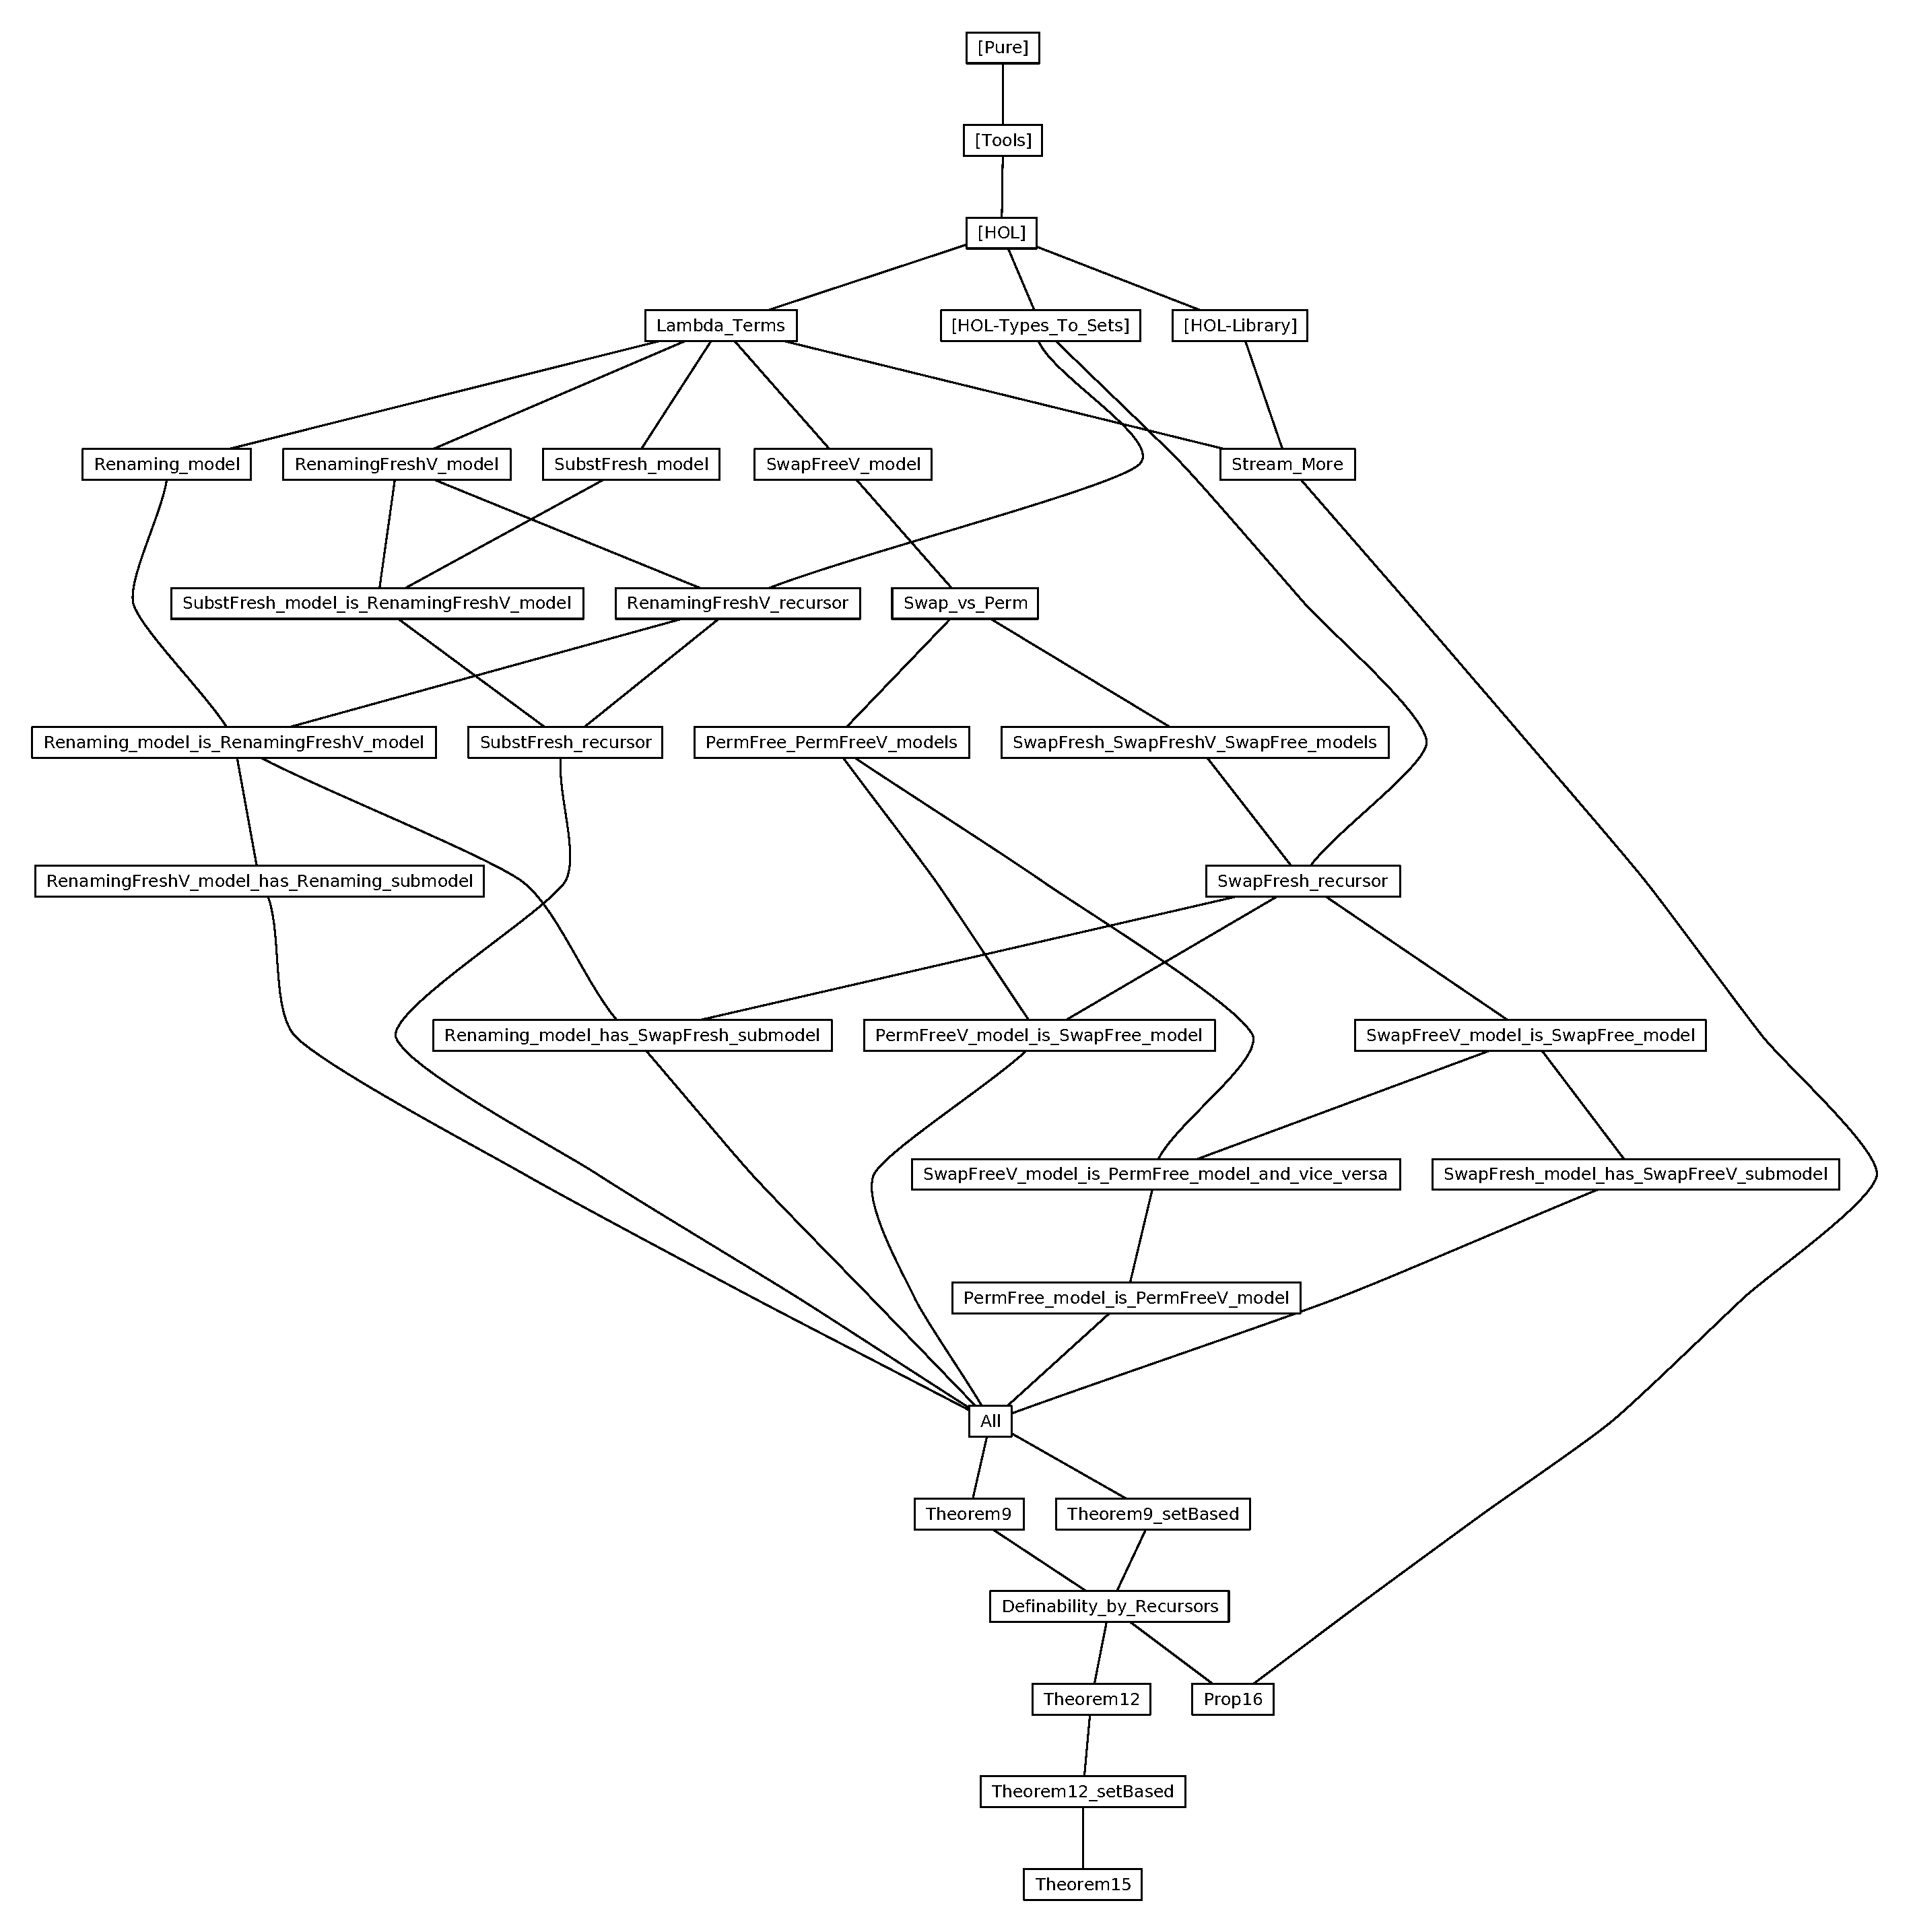
\includegraphics[width=\linewidth]{session_graph.pdf}
	\caption{The Isabelle theories for recursors}
	\label{fig-isabelleTheories}
\end{figure*}


%%%%%

To illustrate this more concretely, let us consider one of the statements of Thm.~\ref{thm-expr}, say $r_4 \geq r_2$, comparing the swap/free recursor $r_4$ with the perm/free variant recursor $r_2$. All the theories we reference below are located in the directory \textsf{Stripped$\_$\allowbreak{}Down} from the archive. The mechanisation of this result has the following components:
\begin{itemize} 
\item The class of models for each recursor corresponds to an Isabelle locale, which fixes a carrier set (as an unspecified type $'D$) and operations on it as indicated by the recursor's signature, and assumes the recursor's characteristic properties (sometimes called ``axioms'' in the paper). Namely:
\begin{itemize} 
     \item The models of $r_2$ (the perm/free variant recursor) are mechanized as the locale $\PermFreeV$ (located in theory \textsf{PermFree$\_$\allowbreak{}PermFreeV$\_$\allowbreak{}models}) which fixes the type (i.e., type variable) $'D$; and on this type it fixes constructors-like operators \textsf{VrD}, \textsf{ApD} and \textsf{LmD}, and permutation- and free-variable-like operators permD and FvarsD, and assumes the model properties required by $r_2$ -- the Isabelle notations for these properties coincide with the ones from the paper, e.g., \PmVr{}, \FvAp{}, etc. 
     %
     \item Similarly, the models of $r_4$ (the swap/free recursor) are mechanized as the locale $\SwapFree$ (located in theory \textsf{SwapFresh$\_$\allowbreak{}SwapFreshV$\_$\allowbreak{}SwapFree$\_$\allowbreak{}models}) which again fixes the necessary model components (carrier $'D$, constructor-like operators \textsf{VrD}, \textsf{ApD} and \textsf{LmD}, and swapping- and free-variable-like operators \textsf{swapD} and \textsf{FvarsD}) and assumes the model properties required by $r_4$ (namely, $\Props_4$)---again, the Isabelle notations match the paper, e.g., \SwFv{}. 
\end{itemize} 
%
\item The definition of an operator, let us refer to it as $F$ (since this will represent an instance of the pre-functor $F$ from the paper's Prop.~\ref{prop-extCriterion}), that maps $r_2$-models (i.e., $(\Sigma_2,\Props_2)$-models) to $r_4$-models (i.e., $(\Sigma_4,\Props_4)$-models), was mechanized as follows:
\begin{itemize} 
      \item In the context of the $\PermFreeV$ locale, which fixes an (arbitrary) $r_2$-model, we defined a swapping-like operator \textsf{swapD} on the carrier $'D$ of that model. (This happened inside the theory \textsf{PermFreeV$\_$\allowbreak{}model$\_$\allowbreak{}is$\_$\allowbreak{}SwapFree$\_$\allowbreak{}model}.) 
      \item Then we proved that \textsf{swapD}, together with the constructor-like and free-variable-like operators (already provided by $r_2$-models), forms an $r_4$-model, i.e., satisfies the  properties $\Props_4$. This happened by first proving all the $\Props_4$ properties in the context of the locale, then using these properties to establish the sublocale relationship $\PermFreeV < \SwapFree$ via the command:
      
\begin{center}
	\begin{tabular}{l}
\textsf{sublocale PermFreeV$\_$\allowbreak{}model $<$ SwapFree$\_$\allowbreak{}model}
\\
\textsf{where swapD = swapD}
\end{tabular} 
\end{center} 

This command (which triggers a proof goal that must be discharged) 
makes the statement that, under the $\PermFreeV$ 
assumptions, i.e., for any $r_2$-model, 
the \textsf{swapD} operator just defined together with the other operators from $\PermFreeV$, 
namely \textsf{VrD}, \textsf{ApD}, \textsf{LmD} and \textsf{FvarsD}, satisfy all the $\SwapFree$ assumptions, i.e., form an 
$r_4$-model. Note that this sublocale relationship implicitly refers to the other operators, in 
other words the above is equivalent to the following command: 

\begin{center}
	\begin{tabular}{l}
		\textsf{sublocale PermFreeV$\_$\allowbreak{}model $<$ SwapFree$\_$\allowbreak{}model}
		\\
		\textsf{where swapD = swapD and VrD = VrD and ApD = ApD} 
		\\
		\textsf{and LmD = LmD and FvarsD = FvarsD}
	\end{tabular} 
\end{center} 

So this sublocale mechanizes the operator $F$. By definition, $F$ leaves unchanged the $(\textsf{VrD},\textsf{ApD},\alb \textsf{LmD})$-part of the models (i.e., factors through the forgetful operators to the constructor-only signature). Also, one can see that together with the identity on morphisms, $F$ is a functor---but we do not mechanize this fact. 
\end{itemize}
%
\item The above locale relationship, showing that $r_2$-models give rise to $r_4$-models (via the above operator $F$), is the core of the ordering $r_4 \geq r_2$. Indeed, taking advantage of this sublocale relationship, we showed that definability via the $r_2$ recursor implies definability via the $r_4$ recursor as follows: In the context of the $\PermFreeV$ locale, i.e., for any $r_2$-model, we showed that the unique morphism of $\Sigma_2$-models guaranteed by $r_2$ coincides (as a function) with the unique morphism to the induced $\Sigma_4$-model guaranteed by $r_4$; indeed, the latter, denoted in the formalisation by $ff0$ (and automatically made available in the $\PermFreeV$ locale via the sublocale relationship), was shown to be a morphism of  $\Sigma_2$-models. (This happened in the theory \textsf{PermFreeV$\_$\allowbreak{}model$\_$\allowbreak{}is$\_$\allowbreak{}SwapFree$\_$\allowbreak{}model}.) Note that, at this stage, $ff0$ had already been available in the context of the $\SwapFree$ locale and known to be the unique morphism between the term model and the (arbitrary) $(\Sigma_4,\Props_4)$-model fixed in the $\SwapFree$ locale.
% (i.e., we had the soundness of $r_4$ already proved -- see point (2) below). 
\end{itemize} 

%%%%%

A similar, but slightly more involved mechanism was used for mechanizing 
the quasi-strength comparison results of Thm.~\ref{thm-qexpr} 
(extended to enhanced recursors in Thm.~\ref{thm-exprEnhanced}). Remember that $r_i \wgeq r_j$ was proved by showing that any $(\Sigma_j,\Props_j)$-model $\MM$ has a $(\Sigma_i,\Props_i)$-submodel---in that there exists a submodel $\MM'$ of $\MM$ that on the one hand still satisfies $\Props_j$, and on the other hand can be regarded as a $(\Sigma_i,\Props_i)$-model (again, via defining on $\MM'$ the $\Sigma_i$-operations). We expressed this in Isabelle as follows: %
Working inside locale $L_j$, we identified a suitable subset $M'$ of $\MM$'s carrier $M$ (and, for enhanced recursors, a suitable subset of $\MM$'s domain 
$D$) and proved that it is closed under the operations and satisfies the $\Props_j$ properties---as discussed in the proof sketch of Thm.~\ref{thm-qexpr}  %{thm-exprEnhanced} 
from App.~\ref{app-proofSketches}, this was in each case a minimal  set closed under the constructors, defined inductively. % using $\MM$'s constructor operators. 
In other words, we built a $(\Sigma_j,\Props_j)$-submodel. To capture this using locales, we defined the locale $L_j'$ that extends $L_j$ with a subset $M'$ that forms a $(\Sigma_j,\Props_j)$-submodel, and proved $L_j \leq L_j'$ by defining $\MM'$ to be the aforementioned minimal submodel of $\MM$.  Then we defined the 
$\Sigma_i$ operations on $M'$ (more precisely, we defined them on the entire type and proved that $M'$ is closed under them), after which we 
proved for them the $\Props_i$ properties. This allowed us  to prove the locale relationship $L_j \leq L_i$, using the submodel $\MM'$ rather than the model $\MM$ as basis for constructing the model for $L_i$. 
These two locale inclusions together 
form a statement of $r_i \wgeq r_j$. Again, this mechanized relationship is effective, in that it allowed us to infer the $r_j$ recursor from the $r_i$ recursor. 


\subsubsection{Mechanization of the recursion theorems}

As a byproduct of the above network of sublocales that allows borrowing recursors, we were able to infer all the nine recursors from just two of them, namely $r_6$ (the swap-fresh recursor) and $r_9$ (the renaming/fresh variant recursor)---as discussed in the proof sketch of Thm.~\ref{thm-allNominalRecs} from 
App.~\ref{app-proofSketches}.  For $r_6$ and $r_9$, we performed direct proofs of initiality. The initial morphism was constructed by first defining inductively a relation and then proving that it is a function and it commutes with the relevant operations and preserves freshness. This approach is distinct from (and we believe simpler than) previous techniques from the literature used to prove nominal recursion  principles. For example, \citet{primrecFOAS-Norrish04} bases the proof of his swap/free recursor on a previous recursor by %Melham and Gordon
 \citet{DBLP:conf/tphol/GordonM96}, which in turn uses the lifting of a function from preterms after proving that it respects $\alpha$-equivalence. Similarly, %Pitts
  \citet{pitts-AlphaStructural}'s proof of the perm/free recursor lifts a function from preterms. 
Our approach is simpler in that it does not delve into preterms, but operates entirely at the abstraction level of terms. 

To illustrate the borrowing process, let us give again a concrete example, considering the swap/fresh recursor $r_6$: In the context of the $\SwapFresh$ locale, i.e., fixing a $(\Sigma_6,\Props_6)$-model, consisting of a type $'D$ and some operators 
\textsf{VrD}, \textsf{ApD}, \textsf{LmD}, \textsf{swapD} and \textsf{freshD} satisfying the $\Props_6$ properties, we proved the existence and uniqueness of a $\Sigma_6$-model morphism from the term model to this (arbitrary) fixed model. This was done by defining a function $ff0$ from terms to $'D$, proving that it is is a morphism of $\Sigma_6$-models (i.e., commutes with the constructors, swapping and freshness operators), and proving that any other morphism of $\Sigma_6$-models must be equal to $ff0$. All this work was performed in the theory \textsf{Swap$\_$\allowbreak{}Fresh$\_$\allowbreak{}recursor}. The relevant theorems (as indicated via comments in the formalization) are called \textsf{ff0$\_$\allowbreak{}Vr}, \textsf{ff0$\_$\allowbreak{}Ap}, \textsf{ff0$\_$\allowbreak{}Lm}, \textsf{ff0$\_$\allowbreak{}swap} and \textsf{ff0$\_$\allowbreak{}fresh} (together stating the morphism property) and \textsf{ff0$\_$\allowbreak{}unique} (stating the uniqueness property). Note that the uniqueness property is actually stated in a stronger form: not only is $ff0$ the unique $\Sigma_6$-morphism, but is even unique among $\Sigmac$-morphisms, i.e., unique among functions commuting with the constructors. 

Now, we could have done direct proofs of soundness for all our recursors (like we did for $r_6$ and $r_9$), but we noticed that we can instead use the expressiveness relationships we discovered between them as a mechanism for \emph{borrowing} soundness from the more expressive ones. However, this was not possible with the relationships as stated in the paper because those already assumed the recursors to be sound (in fact our very notion of recursor assumed soundness); but it \emph{became} possible with a slight generalization of our results. Because this generalization does not bring much conceptually and might have distracted the reader from the main ideas, we decided not to include it in the main paper but to discuss it in the appendix (App.~\ref{app-proofSketches}) as a ``formal engineering optimization''. 

\subsubsection{Theory structure} 

The theory structure of our Isabelle development for recursors is shown in Fig.~\ref{fig-isabelleTheories}.  Everything is based on a formalization of terms as $\alpha$-equivalence classes of preterms, in the theory $\LambdaTerms$. Due to the need to borrow some properties from the terms model to arbitrary models (for given signatures) via the initial morphism (as explained in the proof sketch of Thm.~\ref{thm-qexpr} from App.~\ref{app-proofSketches}), a large theory of terms had to be formalized, comprising a wealth of results about the term operators, depth-based and fresh induction principles. 
%
Moreover, the auxiliary theory $\SwapVsPerm$ performs the conversions between swapping-based and permutation-based axioms: starting with the classic result on switching between the two alternative axiomatizations of nominal sets as described in Pitts's monograph \cite[Section 6.1]{pitts_2013}, and extending this correspondence in various ways as needed by the various recursors: to covering a separate freshness predicate (not reducible to swapping or permutation), to relaxing nominal sets to ``nominal sets modulo $X$'' for a more comprehensive application of Barendregt's convention (as discussed in App.~\ref{app-addingBacknhancements}), etc. 

The names of the  other theories in Fig.~\ref{fig-isabelleTheories} are 
self-explanatory. For example:
\begin{mmyitem}
\item the theory $\RenamingFreshV$ formalizes the models for the renaming/fresh variant recursor (and of course contains the locale with the same name);
%
\item the theory $\SwapSeveral$ formalizes the models corresponding to the swap/fresh, swap/fresh variant and swap/free recursors (and contains the corresponding locales); 
%
\item the theory $\RenamingIsRenamingFreshV$ proves that each renaming model is (can be regarded as) a renaming/fresh variant model, via the sublocale statement $\Renaming \leq \RenamingFreshV$; 
%
\item the theory $\SwapFreshHasSwapFreeV$ proves that each swap/fresh model has a swap/fresh submodel that is (can be regarded as) a swap/freee variant model, via the sublocale statements 
$\SwapFresh \leq \SwapFreshSM$ and $\SwapFresh \leq \SwapFreeV$. 
\end{mmyitem}

Note that there are three theories whose names refer explicitly to a recursor: $\RenamingFreshVR$, $\SwapFreshR$ and 
$\SubstFreshR$. The first two of these contain direct formalizations of the renaming/fresh variant and swap/fresh recursors. As discussed in the proof sketch of Thm.~\ref{thm-allNominalRecs}
in App.~\ref{app-proofSketches}, these two recursors (which are at the top of the $\geq$ hierarchy) have been used to derive all the other recursors. In all but one case, we have performed this derivation right after the sublocale result that enables it. For example, the swap/free variant recursor is derived from the swap/fresh recursor in theory  $\SwapFreshHasSwapFreeV$, right after the sublocale relationship $\SwapFresh \leq \SwapFreeV$ is established. 
The exception is the subst/fresh recursor, to which we dedicated its own theory $\SubstFreshR$---this was done in order to highlight the slightly more involved structure of the borrowing argument, which requires fresh induction. 

The theory $\ThAll$ imports all the relevant top theories (and a few of the relevant non-top ones for better documentation) and contains comments that map the formalization to the paper.\footnote{For the theories that are located in the figure below \textsf{All}, i.e., import  this theory, please see \S\ref{app-subsec-localeFree}.}



\subsection{Mechanization of the negative results} 
\label{subsec-neg}
%
The two negative results expressed in Prop.~\ref{prop-negRec} are mechanized in the theory \textsf{Prop16}.  
The mechanized statement follows closely the presentation from \S\ref{subsec-negResRec}, in each case stating that there exist morphisms definable by one recursor but not by the other. 
%
The mechanized proofs  also follow closely Prop.~\ref{prop-negRec}'s proof sketch given in the paper (and the extended proof sketch given in App.~\ref{app-proofSketches}). For each of the two $r_i \not\geq r_j$ results, we:
(1) build a $(\Sigma_j,\Props_j)$-model (and prove that it is indeed a $(\Sigma_j,\Props_j)$-model), 
and (2) show that there exists no extension of 
	the $\Sigmac$-part of that model to a $(\Sigma_i,\Props_i)$-model. 
(In each case, such an extension would consist of freeness and permutation operators that, together with the constructor-like operators, satisfy the $\Props_i$-properties.) 


\subsection{Mechanization of the results about corecursors}
\label{subapp-isa-corecursors}

Our approach to mechanizing the corecursors is similar to that we took for recursors. Namely,  we have a locale for each of the eight types of models underlying the nominal corecursors, as shown in Fig.~\ref{fig-localesCoRec}. In a corecursor context, in the formalization (unlike in the paper) we use the term ``comodel'' rather than ``model''. 
% in order to remember that we are in the ``co'' world.

\newcommand\PermFreeCo{\small \textsf{PermFree$\_$\allowbreak{}comodel}}
\newcommand\PermFreeVCo{\small \textsf{PermFreeV$\_$\allowbreak{}comodel}}
\newcommand\SwapFreeVCo{\small \textsf{SwapFreeV$\_$\allowbreak{}comodel}}
%\newcommand\SwapFreeCo{\small \textsf{SwapFree$\_$\allowbreak{}comodel}}
\newcommand\SwapFreshVCo{\small \textsf{SwapFreshV$\_$\allowbreak{}comodel}}
\newcommand\SwapFreshCo{\small \textsf{SwapFresh$\_$\allowbreak{}comodel}}
\newcommand\SwapFreshSMCo{\small \textsf{submodel$\_$\allowbreak{}SwapFresh$\_$\allowbreak{}comodel}}
\newcommand\SubstFreshCo{\small \textsf{SubstFresh$\_$\allowbreak{}comodel}}
\newcommand\RenamingCo{\small \textsf{Renaming$\_$\allowbreak{}comodel}}
\newcommand\RenamingFreshVCo{\small \textsf{RenamingFreshV$\_$\allowbreak{}comodel}}


\begin{figure}
	\centering
	\begin{tabular}{c|c}
		Corecursor & Corresponding locale
		\\\hline 
		$\ccr_1$ (perm/free) & $\PermFreeCo$
		\\
		$\ccr_2$ (perm/free variant) &  $\PermFreeVCo$
		\\
		$\ccr_3$ (swap/free variant) & $\SwapFreeVCo$
	%	\\
	%	$\ccr_4$ (swap/free) & $\SwapFreeCo$
		\\
		$\ccr_5$ (swap/fresh variant) & $\SwapFreshVCo$
		\\
		$\ccr_6$ (swap/fresh) &  $\SwapFreshCo$
		\\
		$\ccr_7$ (subst/fresh) & $\SubstFreshCo$
		\\
		$\ccr_8$ (renaming) & $\RenamingCo$
		\\
		$\ccr_9$ (renaming fresh variant) &  $\RenamingFreshVCo$
		\\
	\end{tabular}
	\caption{Isabelle locales corresponding to corecursors}
	\label{fig-localesCoRec}
\end{figure}

The proof of Thm.~\ref{thm-exprCo} shows that 
one corecursor is stronger than another, say $\ccr_i \geq \ccr_j$, by transforming $(\Sigma_j,\Props_j)$-models to $(\Sigma_i,\Props_i)$-models; always the carrier is the same, and the specific $\Sigma_i$-operators are defined. Again this is done by working inside a locale $L_j$, which represents $(\Sigma_j,\Props_j)$-models by fixing $\Sigma_j$ operators and assuming the $\Props_j$ properties. Inside this locale, we define the $\Sigma_i$-operations and infer the $\Props_i$ properties from $\Props_j$. This allows us to prove the sublocale relationship $L_j \leq L_i$, where $L_i$ is the locale representing $(\Sigma_i,\Props_i)$-models. So $\ccr_i \geq \ccr_j$ is formalized as $L_j \leq L_i$.  This again allowed us to borrow for $(\Sigma_j,\Props_j)$-models the $r_i$ corecursor, in other words to infer the $r_j$ corecursor from the $r_i$ corecursor. 

\begin{figure*}
	\centering
	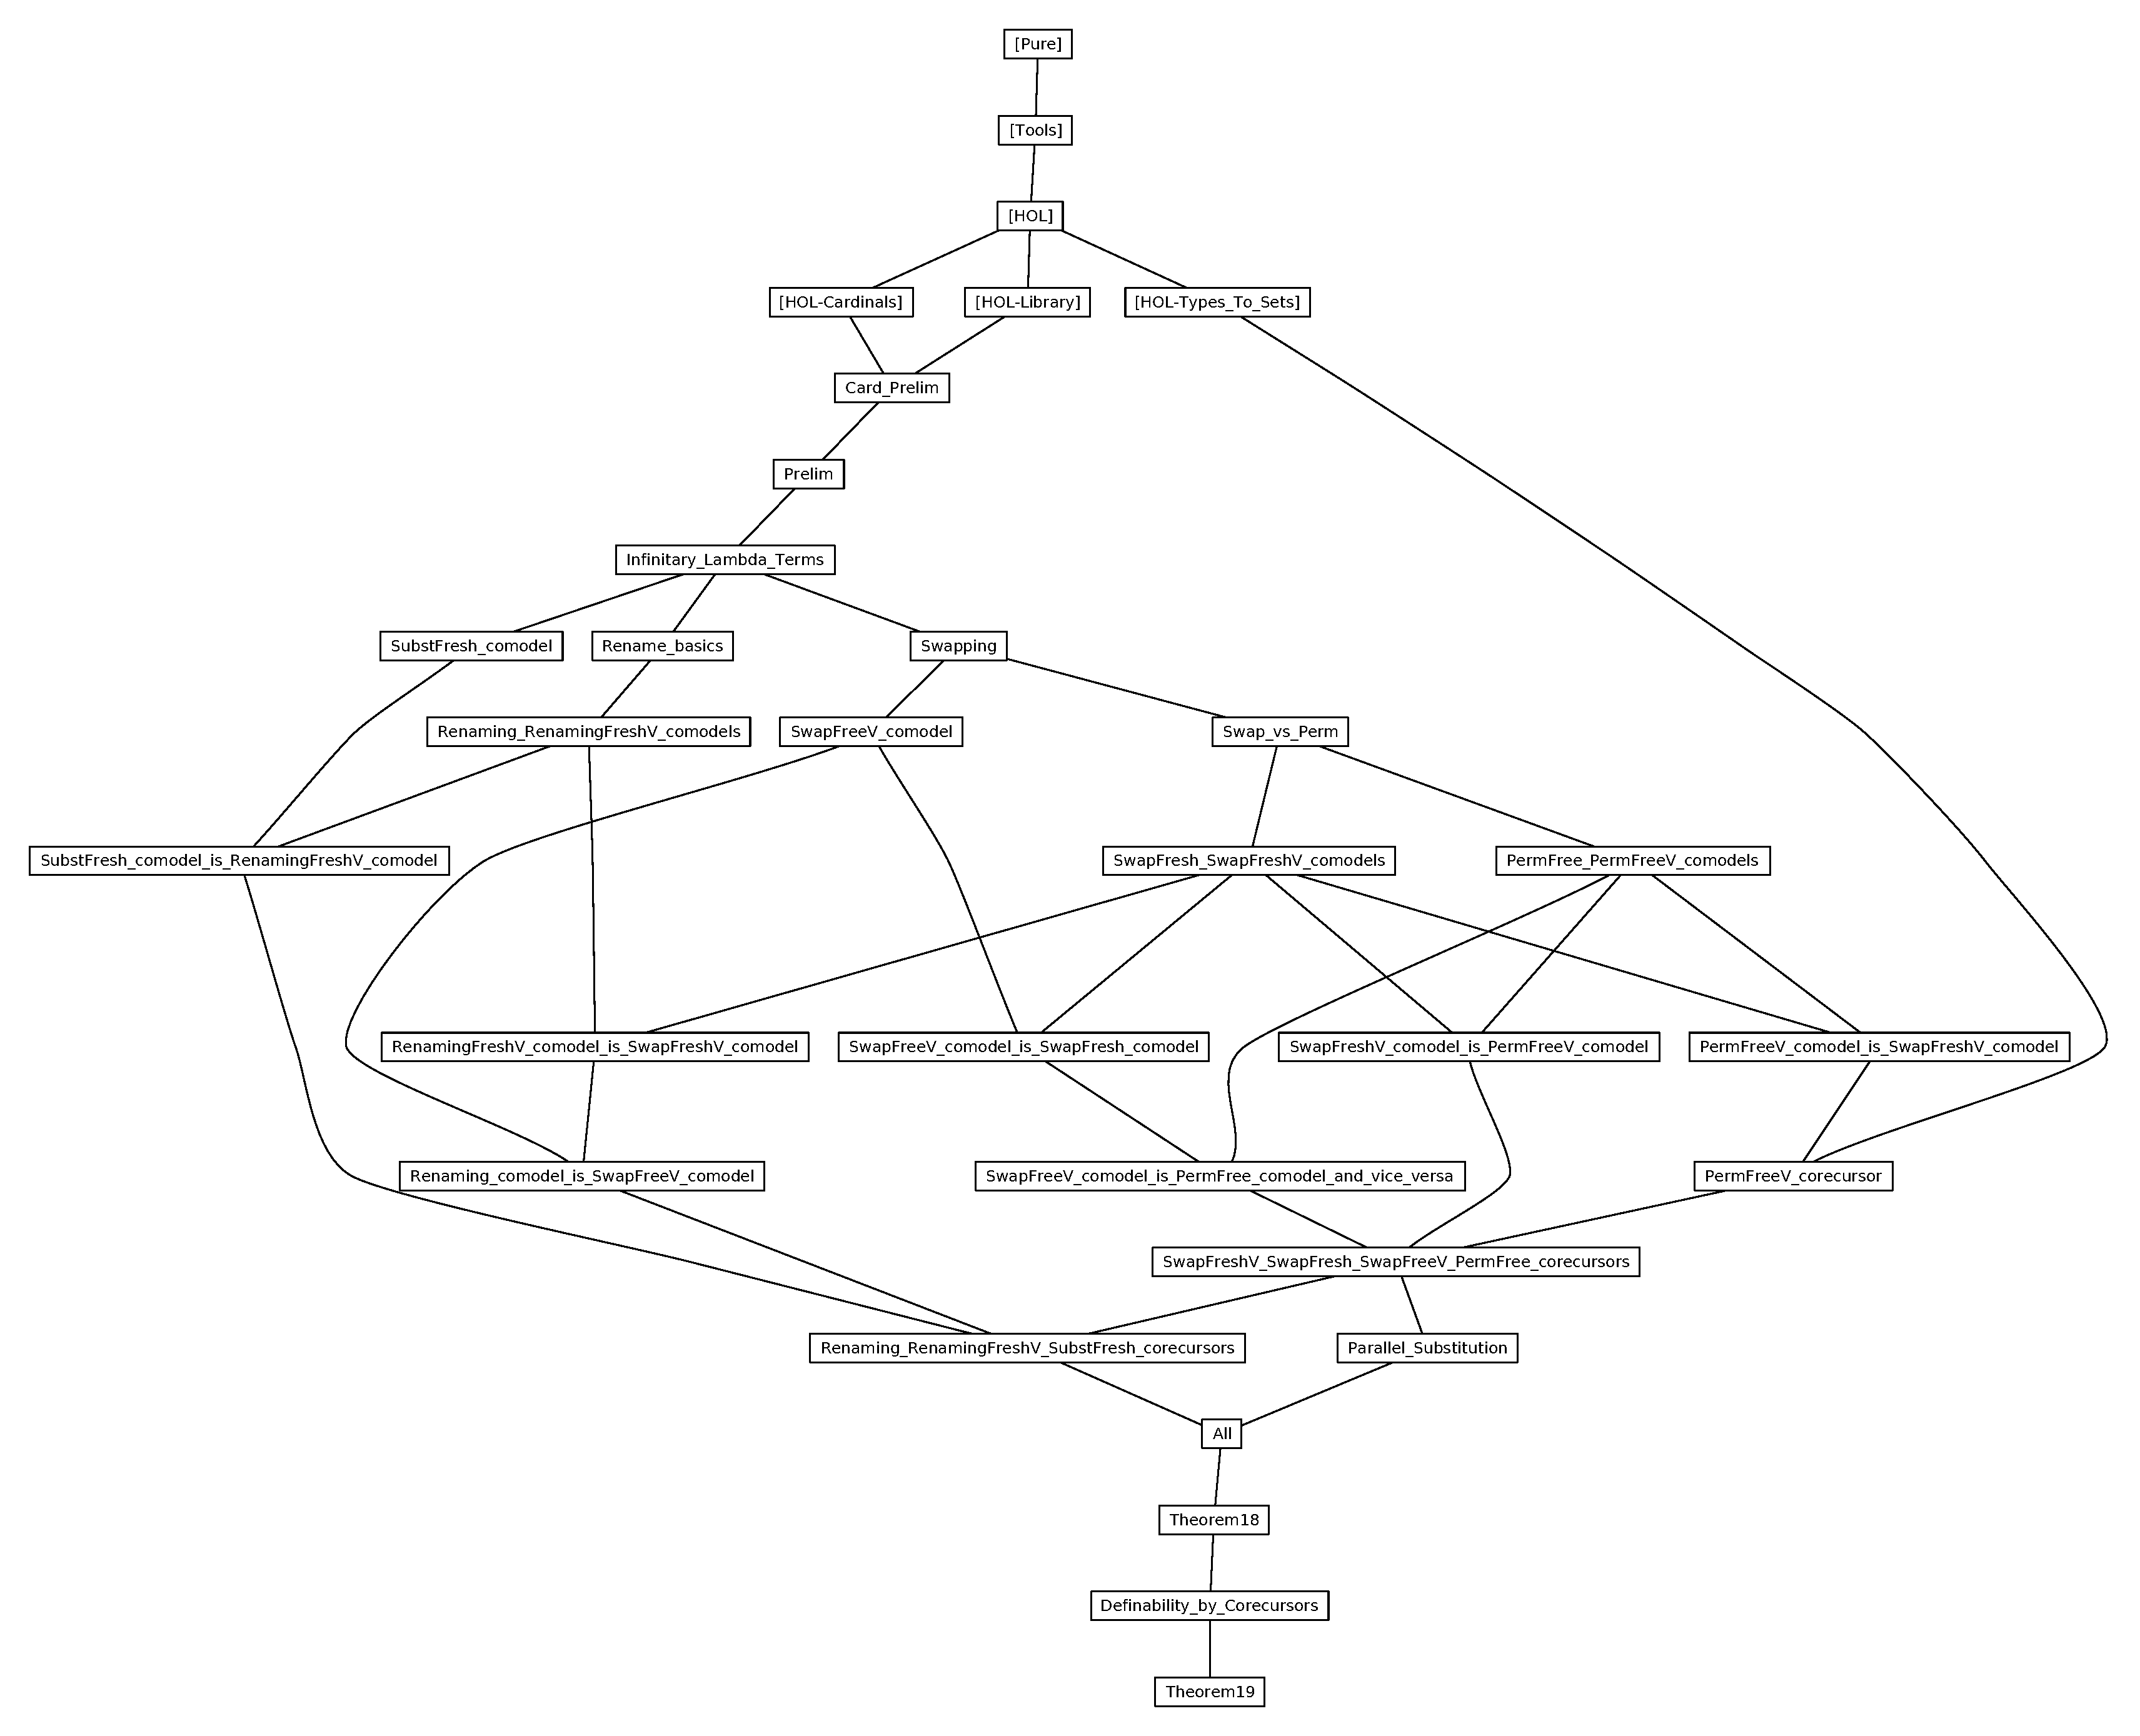
\includegraphics[width=\linewidth]{cosession_graph.pdf}
	\caption{The Isabelle theories for corecursors}
	\label{fig-isabelleCoTheories}
\end{figure*}

This sublocale hierarchy of locales, which matches exactly the $\geq$-hierarchy of Thm.~\ref{thm-exprCo}, allowed us to (1) prove the corecursion principle for $\ccr_2$ (which is at the top of the hierarchy), and infer all the others from it along sublocale relationships---as discussed in the proof sketch of Thm.~\ref{thm-allNominalCoRecs} from 
App.~\ref{app-proofCoSketches}.  

\newcommand\ParallelSubstitution
{\small \textsf{Parallel$\_$\allowbreak{}Substitution}}
\newcommand\InfinitaryLambdaTerms
{\small \textsf{Infinitary$\_$\allowbreak{}Lambda$\_$\allowbreak{}Terms}}
%\newcommand\SwapVsPerm
%{\small \textsf{Swap$\_$\allowbreak{}vs$\_$\allowbreak{}Perms}}
\newcommand\CoSwapSeveral
{\small \textsf{SwapFresh$\_$\allowbreak{}SwapFreshV$\_$\allowbreak{}comodels}}
\newcommand\RenamingIsSwapFreeV
{\small \textsf{Renaming$\_$\allowbreak{}comodel$\_$\allowbreak{}is$\_$\allowbreak{}SwapFreeV$\_$\allowbreak{}comodel}}


\newcommand\CoPermFreeVR
{\small \textsf{PermFreeV$\_$\allowbreak{}corecursor}}

\newcommand\CoSeveralR
{\small \textsf{SwapFreshV$\_$\allowbreak{}SwapFresh$\_$\allowbreak{}SwapFreeV$\_$\allowbreak{}PermFree$\_$\allowbreak{}corecursors}}

\newcommand\CoSeveralTR
{\small \textsf{Renaming$\_$\allowbreak{}RenamingFreshV$\_$\allowbreak{}SubstFresh$\_$\allowbreak{}corecursors}}

\newcommand\CoSwapFreeV{\small \textsf{SwapFreeV$\_$\allowbreak{}comodel}}


The theory structure of our Isabelle development for corecursors is shown in Fig.~\ref{fig-isabelleCoTheories}.  
The formalization of iterms as equivalence classes of pre-iterms and of all the operators and proof principles described in \S\ref{app-detailsIterms} is performed in the theory $\InfinitaryLambdaTerms$. 


The names of the  other theories in Fig.~\ref{fig-isabelleCoTheories} are again
self-explanatory. For example:
\begin{mmyitem}
	\item the theory $\CoSwapFreeV$ formalizes the swap/free models (and contains the locale \\ $\SwapFreeVCo$); 
		
	\item the theory $\CoSwapSeveral$ formalizes the swap/fresh and swap/fresh variant models (and contains the corresponding locales); 

	%
	\item the theory $\RenamingIsSwapFreeV$ proves that each renaming model is (can be regarded as) a swap/free variant model, via the sublocale statement $\RenamingCo \leq \SwapFreeVCo$. 
	%
\end{mmyitem}

There are three theories whose names refer explicitly to  corecursors.  
$\CoPermFreeVR$ contains the direct formalization of the perm/free corecursor, i.e., the proof of the finality principle as discussed in the proof sketch of Thm.~\ref{thm-allNominalCoRecs}
from App.~\ref{app-proofCoSketches}. This corecursor (which is at the top of the $\geq$ hierarchy) has been used to derive all the other seven corecursors. These derivations happen along the corresponding sublocale relationships in the theories 
\\$\CoSeveralR$ and \\$\CoSeveralTR$.

The theory $\ParallelSubstitution$ contains the definition of parallel substitution on iterms using the swap/fresh variant corecursor $\ccr_5$ (as discussed in \S\ref{app-exaCorec}). The full-recursion enhancement of the swap/fresh variant corecursor described in \S\ref{app-enhCorec} is performed at the end of the theory \\$\CoSeveralR$. 

Again, there is a theory $\ThAll$ that imports the relevant top theories and has comments connecting the formalization to the paper.\footnote{For the theories that are located in the figure below \textsf{All}, i.e., import  this theory, we again refer the reader to  \S\ref{app-subsec-localeFree}.}




\subsection{Locale-free, top-level statements of the main results}
\label{app-subsec-localeFree}

%\subsection{Locale-free statements of the results, matching closely the paper} 


We would like to stress that our mechanization, while walking a tight rope in order to minimize the number of recursion principles that are proved  directly (without borrowing), does \emph{not} suffer from any bootstrapping problem or incur any additional assumptions. Rather, it certifies 
Thms.~\ref{thm-allNominalRecs}, \ref{thm-expr}, \ref{thm-qexpr}, 
\ref{thm-allNominalCoRecs} and \ref{thm-exprCo} from the main paper (and also Thms.~\ref{thm-allNominalRecsEnhanced} and \ref{thm-exprEnhanced} from the appendix) 
as they are claimed in the paper, but %(in the case of the theorems) 
using the Isabelle locale jargon. (And Prop.~\ref{prop-negRec} has a faithful formalization as well, but that does not make use of locales---see \S\ref{subsec-neg}.) 

For readers who are interested in inspecting the mechanized statements of the results but not in understanding the locale jargon, we have also reformulated the results in a manner that matches closely the statements from the main paper. 

In Fig.~\ref{fig-isabelleTheories} (for recursors), the locale-free statements are in the theories that inherit $\ThAll$, culminating with theories that have suggestive names, namely \textsf{Theorem9}, \textsf{Theorem12}, \textsf{Theorem15} and \textsf{Prop16}.  The main results in these theories, which can be found using the keyword ``theorem'', 
are statements of Thm.~\ref{thm-allNominalRecs}, Thm.~\ref{thm-expr},  Thm.~\ref{thm-qexpr} and Prop.~\ref{prop-negRec} that, just like their paper counterparts, 
refer to the nominal recursors $r_i$ using their epi-recursor structure and the notion of definability (introduced in the theory \textsf{Definability$\_$\allowbreak{}by$\_$\allowbreak{}Recursors}).  Most of the results are formalized using categories of models assumed to have the carrier sets as the entire type (which is very convenient in HOL formalizations); however, for Thm.~\ref{thm-qexpr} and one half of Prop.~\ref{prop-negRec}, we need the greater flexibility offered by considering explicit carrier sets (as subsets of the underlying types), so we formalized the set-based versions of these categories as well.  

For example, the part of Thm.~\ref{thm-allNominalRecs} that refers to $r_1$ states the recursion (initiality) principle as follows 
(in theory \textsf{Theorem9}): 

\medskip
\noindent 
\textsf{
theorem init$\_$\allowbreak{}I1:
\\
 \hspace*{3ex}isObjectC1 (VrD,ApD,LmD,permD,FvarsD) $\LRA$
\\
\hspace*{3ex}$\exists!$G. isMorphismC1 G I1 (VrD,ApD,LmD,permD,FvarsD)"
}
\medskip 

This states that for any object of the category \textsf{C1} (the category of models for $r_1$), 
there exists a unique morphism \textsf{G} from the term model \textsf{I1} to  \textsf{C1}. 
Note that an object in  \textsf{C1} is a tuple (VrD,ApD,LmD,permD,FvarsD) consisting of 
constructor-like, permutation-like and free-variable-like operators on a carrier type (not shown 
explicitly in the tuple). The predicates \textsf{isObjectC1} and \textsf{isMorphismC1} are defined appropriately 
(in particular, the models are required to satisfy the $\Props_1$ properties), and shown to form a category 
(via a separate Isabelle statement). The model \textsf{I1} is defined as the term model for the signature $\Sigma_1$:

\medskip 
\noindent
\textsf{
definition I1 where I1 = (Vr, Ap, Lm, perm, Fvars)
}
\medskip

Indeed, \textsf{Vr}, \textsf{Ap}, \textsf{Lm}, \textsf{perm}, \textsf{Fvars} are defined to be the standard operators on terms. 
%

In fact, we define all the components of the epi-recursor $r_1$ = \textsf{(B,T,C1,I1,R1)}: the base category \textsf{B} and its 
base object \textsf{T}, the category \textsf{C1} and its object \textsf{I1}, the functor \textsf{R1}, and wee prove that 
they are indeed categories and functor, that \textsf{R1} applied objects to \textsf{I1} yields \textsf{T}, etc. In short, 
\textsf{(B,T,C1,I1,R1)} is shown to be an epi-recursor. And the same is done for all the other recursor $r_i$. All this is done 
in theory \textsf{Theorem9}. 

The recursion theorem is alternatively expressed in combinator form (also in theory \textsf{Theorem9}): 

\medskip 
\noindent 
\textsf{
theorem REC1$\_$\allowbreak{}I1: 
\\
\hspace*{3ex}isObjectC1 (VrD,ApD,LmD,permD,FvarsD) $\LRA$ 
\\
\hspace*{3ex}isMorphismC1 (REC1 VrD ApD LmD) I1 (VrD,ApD,LmD,permD,FvarsD)
}
\medskip 

The above says that \textsf{REC1 VrD ApD LmD} is the unique morphism from the term model \textsf{I1} to the model \textsf{(VrD,ApD,LmD,permD,FvarsD)}. 
Note that the combintor \textsf{REC1} only depends on the constructor-like operators 
\textsf{VrD}, \textsf{ApD} and \textsf{LmD}, and not on the other two operators, \textsf{permD} and \textsf{FvarsD}; 
however, the fact that \textsf{REC1 VrD ApD LmD} is a morphism between \textsf{I1} and 
\textsf{(VrD,ApD,LmD,permD,FvarsD)} of course relies crucially on \textsf{permD} and \textsf{FvarsD} and the $\Props_1$ properties. 

\medskip 
Definability by recursor $r_1$ is expressed as follows (in theory \textsf{Definablity$\_$\allowbreak{}by$\_$\allowbreak{}Recursors}):\footnote{``\textsf{fun}'' is another way of introducing definitions in Isabelle. We prefer it here because, unlike ``\textsf{definition}'', it allows pattern matching.}  

\medskip 
\noindent 
\textsf{
fun definableByR1 where 
\\\hspace*{3ex}definableByR1 f (VrD,ApD,LmD) = 
\\\hspace*{3ex}$\exists$permD FvarsD. isObjectC1 (VrD,ApD,LmD,permD,FvarsD) $\wedge$ 
f = REC1 VrD ApD LmD
}
\medskip 

Thus, for a morphism \textsf{f} between the term $\Sigmac$-model and 
another $\Sigmac$-model (VrD,ApD,LmD), the definability predicate says that there exists a extension of (VrD,ApD,LmD) 
to a \textsf{C1} object \textsf{(VrD,ApD,LmD,permD,FvarsD)}  (i.e., a $(\Sigma_1,\Props_1)$-model) 
such that $f$ can be defined as the unique morphism between the term $(\Sigma_1,\Props_1)$-model 
and \textsf{(VrD,ApD,LmD,permD,FvarsD)}  (namely, using the \textsf{REC1} combinator). The above is done for all the recursors $r_i$.

Now, for example, the $r_5 \geq r_4$ part of Thm.~\ref{thm-expr} is expressed just like in the paper, 
but expanding the definition of $\geq$, 
as an implication between definabilities (in theory \textsf{Theorem12}): 

\medskip 
\noindent 
\textsf{
	theorem r5$\_$\allowbreak{}ge$\_$\allowbreak{}r4:
	\\\hspace*{3ex}definableByR4 f (VrD, ApD, LmD) $\LRA$
	\\\hspace*{3ex}definableByR5 f (VrD, ApD, LmD)
} 
\medskip 

And the $r_2 \not\geq r_4$ part of Prop.~\ref{prop-negRec} is expressed again like in the paper with the definition of $\geq$ expanded, 
stating the existence of an \textsf{f} definable by $r_4$ but not by $r_2$ (in theory \textsf{Prop16}): 

\medskip 
\noindent 
\textsf{
theorem not$\_$\allowbreak{}r2$\_$\allowbreak{}ge$\_$\allowbreak{}r4: 
	\\\hspace*{3ex}$\exists$f. definableByR4 f (VrD, ApD, LmD) $\wedge$ $\neg$ definableByR2 f (VrD, ApD, LmD)
}
\medskip 

\noindent 
\textit{Set-based versions of the concepts.}  
While working with models as tuples of operators on the entire type (i.e., assuming that the carrier of the model 
is an entire type) does not lose generality, sometimes we need more flexibility---for example, when we wish to consider 
submodels, whose carriers are usually not the entire type. Making disjoint copies and performing type definitions 
could get us by, but in these cases it is more convenient to employ a more flexible, ``set-based'' version of the models, 
with explicit carrier sets. In this more flexible setting, for example the models for $r_1$ are now 
\textsf{(D,VrD,ApD,LmD,permD,FvarsD)} which in  addition to the operators also feature a subset \textsf{D} of the carrier 
type, assumed to be closed under these operators, e.g., \textsf{ApD d1 d2} $\in$ D whenever \textsf{d1,d2} $\in$ \textsf{D}. 
We use primed notation to indicate these set-based concepts, e.g., \textsf{isObjectC1'}, 
\textsf{definableByR1'}, etc. While the primed versions are semantically equivalent to the originals, they are needed for modeling certain phenomena in a more finite-grained manner. They are formalized in 
the theories \textsf{Set$\_$\allowbreak{}Based$\_$\allowbreak{}Recursors} and  \textsf{Definablity$\_$\allowbreak{}by$\_$\allowbreak{}Recursors}.

The theory \textsf{Theorem12$\_$\allowbreak{}setBased} infers the set-based version of Thm.~\ref{thm-expr} by transferring to sets the results from theory \textsf{Theorem12}.  
For example, the $r_5 \geq r_4$ part of Thm.~\ref{thm-expr} 
is expressed as follows in the set-based setting (in theory \textsf{Theorem12$\_$\allowbreak{}setBased}): 

\medskip 
\noindent 
\textsf{
	theorem r5$\_$\allowbreak{}ge$\_$\allowbreak{}r4':
	\\\hspace*{3ex}definableByR4' f (D, VrD, ApD, LmD) $\LRA$
	\\\hspace*{3ex}definableByR5' f (D, VrD, ApD, LmD)
} 
\medskip 

The primed set-based versions yield the original versions, e.g., \textsf{r5$\_$\allowbreak{}ge$\_$\allowbreak{}r4'} yields \textsf{r5$\_$\allowbreak{}ge$\_$\allowbreak{}r4} by taking \textsf{D} to be universal set (comprising the entire type).  


Because the $r_1 \not\geq r_2$ part of Prop.~\ref{prop-negRec} requires a set defined by a predicate, 
we also formalize it using the more general primed models. Namely, after defining 
a particular $(\Sigma_2,\Props_2)$-model as described in the proof of Prop.~\ref{prop-negRec}, 
which in the formalization we call \textsf{(E,VrE,ApE,LmE)}, we prove:\footnote{So in the following statement, \textsf{E,VrE,ApE,LmE} are \emph{not} universally quantified variables (as are, for example, \textsf{D,VrD,ApD,LmD} in the theorem \textsf{r5$\_$\allowbreak{}ge$\_$\allowbreak{}r4'} above), but certain defined constants.}

\medskip 
\noindent 
\textsf{
	theorem not$\_$\allowbreak{}r1$\_$\allowbreak{}ge$\_$\allowbreak{}r2: 
	\\\hspace*{3ex}$\exists$f. definableByR2' f (E, VrE, ApE, LmE) $\wedge$ $\neg$ definableByR1' f (E, VrE, ApE, LmE)
}
\medskip 


The same is true for Thm.~\ref{thm-qexpr}, where we must consider initial segments formed by submodels.  For example, the 
$r_6\wgeq r_8$ part of Thm.~\ref{thm-qexpr} is formalized as follows (in theory \textsf{Theorem15}): 

\medskip 
\noindent 
\textsf{
theorem r6$\_$\allowbreak{}quasi$\_$\allowbreak{}ge$\_$\allowbreak{}r8':
\\\hspace*{3ex}definableByR8' g (D, VrD, ApD, LmD) $\LRA$  
\\\hspace*{3ex}$\exists$g0. isMorphismB' g0 T' (ob' (D, VrD, ApD, LmD)) $\wedge$ 
\\\hspace*{3ex}\phantom{$\exists$}
g = mo' (D, VrD, ApD, LmD) $\circ$ g0 $\wedge$
\\\hspace*{3ex}\phantom{$\exists$}
definableByR6' g0 (ob' (D, VrD, ApD, LmD))
}
\medskip 

Its formulation matches that from the paper, but again expands the definition of $\wgeq$: \textsf{mo'} 
and \textsf{ob'} formalize the initial segment $(\Bcat_0,(m(B):o(B)\ra B)_{B \in \Obj{\Bcat}})$ from Def.~\ref{defi-qstrong} 
(where \textsf{mo'}  is the morphism operator $m$ and \textsf{ob'} is the object operator $o$). 
For all the $\wgeq$ relationships stated in the theorem, \textsf{ob'}, when applied to an object of the category \textsf{B'}, 
returns its minimal submodel  % from App.~\ref{app-proofSketches}), 
and \textsf{mo'} returns the inclusion morphism (as explained in the proof sketch of Thm.~\ref{thm-qexpr}). These are proved to form an initial segment of \textsf{B'}. 
So the above theorem says that any morphism \textsf{g} definable by $r_8$ can be written as a composition 
between the initial-segment morphism and a morphism \textsf{g0} definable by $r_6$ (like in the definition of $\wgeq$). 
Because this composition involves submodels, the definablity of \textsf{g0} must be expressed using the set-based version. This is why we shift to the set-based setting completely, and  
the morphisms \textsf{g0} and \textsf{g} dwell the set-based version of the base category. 





\bigskip 
In Fig.~\ref{fig-isabelleCoTheories} (for corecursors), the locale-free statements are again in the theories that inherit 
$\ThAll$, culminating with theories that have suggestive names, namely \textsf{Theorem18} and \textsf{Theorem19}. 
The main results, which can again be found using the keyword ``theorem'',  
are statements of Thm.~\ref{thm-allNominalCoRecs} and Thm.~\ref{thm-exprCo}. Similarly to the case of recursors, we 
use concepts and terminology that matches the paper closely.  

The formalization follows a similar pattern to the one 
for recursors. For example, the $\ccr_5 \geq \ccr_6$ part of Thm.~\ref{thm-exprCo} is expressed as follows (in theory \textsf{Theorem19}): 

\medskip 
\noindent 
\textsf{
	theorem cr5$\_$\allowbreak{}ge$\_$\allowbreak{}cr6:
	\\\hspace*{3ex}definableByCR6 f DestD $\LRA$
	\\\hspace*{3ex}definableByCR5 f DestD
} 


% End original appendix.tex


%%%%%%%%%%%%%%%%%%%%%%%%%

%%% -*-BibTeX-*-
%%% Do NOT edit. File created by BibTeX with style
%%% ACM-Reference-Format-Journals [18-Jan-2012].

\begin{thebibliography}{64}

%%% ====================================================================
%%% NOTE TO THE USER: you can override these defaults by providing
%%% customized versions of any of these macros before the \bibliography
%%% command.  Each of them MUST provide its own final punctuation,
%%% except for \shownote{}, \showDOI{}, and \showURL{}.  The latter two
%%% do not use final punctuation, in order to avoid confusing it with
%%% the Web address.
%%%
%%% To suppress output of a particular field, define its macro to expand
%%% to an empty string, or better, \unskip, like this:
%%%
%%% \newcommand{\showDOI}[1]{\unskip}   % LaTeX syntax
%%%
%%% \def \showDOI #1{\unskip}           % plain TeX syntax
%%%
%%% ====================================================================

\ifx \showCODEN    \undefined \def \showCODEN     #1{\unskip}     \fi
\ifx \showDOI      \undefined \def \showDOI       #1{#1}\fi
\ifx \showISBNx    \undefined \def \showISBNx     #1{\unskip}     \fi
\ifx \showISBNxiii \undefined \def \showISBNxiii  #1{\unskip}     \fi
\ifx \showISSN     \undefined \def \showISSN      #1{\unskip}     \fi
\ifx \showLCCN     \undefined \def \showLCCN      #1{\unskip}     \fi
\ifx \shownote     \undefined \def \shownote      #1{#1}          \fi
\ifx \showarticletitle \undefined \def \showarticletitle #1{#1}   \fi
\ifx \showURL      \undefined \def \showURL       {\relax}        \fi
% The following commands are used for tagged output and should be
% invisible to TeX
\providecommand\bibfield[2]{#2}
\providecommand\bibinfo[2]{#2}
\providecommand\natexlab[1]{#1}
\providecommand\showeprint[2][]{arXiv:#2}

\bibitem[\protect\citeauthoryear{Abel, Momigliano, and Pientka}{Abel
  et~al\mbox{.}}{2017}]%
        {poplmarkReloaded}
\bibfield{author}{\bibinfo{person}{Andreas Abel}, \bibinfo{person}{Alberto
  Momigliano}, {and} \bibinfo{person}{Brigitte Pientka}.}
  \bibinfo{year}{2017}\natexlab{}.
\newblock \showarticletitle{{POPLMark Reloaded}}.
\newblock In \bibinfo{booktitle}{\emph{{Logical Frameworks and Meta-Languages:
  Theory and Practice (LFMTP)} 2017}},
  \bibfield{editor}{\bibinfo{person}{Marino Miculan} {and}
  \bibinfo{person}{Florian Rabe}} (Eds.).
\newblock
\urldef\tempurl%
\url{https://lfmtp.org/workshops/2017/inc/papers/paper_8_abel.pdf}
\showURL{%
\tempurl}


\bibitem[\protect\citeauthoryear{Aczel, Ad{\'{a}}mek, Milius, and
  Velebil}{Aczel et~al\mbox{.}}{2003}]%
        {DBLP:journals/tcs/AczelAMV03}
\bibfield{author}{\bibinfo{person}{Peter Aczel}, \bibinfo{person}{Jir{\'{\i}}
  Ad{\'{a}}mek}, \bibinfo{person}{Stefan Milius}, {and} \bibinfo{person}{Jiri
  Velebil}.} \bibinfo{year}{2003}\natexlab{}.
\newblock \showarticletitle{Infinite trees and completely iterative theories: a
  coalgebraic view}.
\newblock \bibinfo{journal}{\emph{Theor. Comput. Sci.}} \bibinfo{volume}{300},
  \bibinfo{number}{1-3} (\bibinfo{year}{2003}), \bibinfo{pages}{1--45}.
\newblock
\urldef\tempurl%
\url{https://doi.org/10.1016/S0304-3975(02)00728-4}
\showDOI{\tempurl}


\bibitem[\protect\citeauthoryear{Allais, Chapman, McBride, and McKinna}{Allais
  et~al\mbox{.}}{2017}]%
        {allais-bindingsByDependentTypes-agda}
\bibfield{author}{\bibinfo{person}{Guillaume Allais}, \bibinfo{person}{James
  Chapman}, \bibinfo{person}{Conor McBride}, {and} \bibinfo{person}{James
  McKinna}.} \bibinfo{year}{2017}\natexlab{}.
\newblock \showarticletitle{Type-and-scope safe programs and their proofs}. In
  \bibinfo{booktitle}{\emph{Proceedings of the 6th {ACM} {SIGPLAN} Conference
  on Certified Programs and Proofs, {CPP} 2017, Paris, France, January 16-17,
  2017}}, \bibfield{editor}{\bibinfo{person}{Yves Bertot} {and}
  \bibinfo{person}{Viktor Vafeiadis}} (Eds.). \bibinfo{publisher}{{ACM}},
  \bibinfo{pages}{195--207}.
\newblock
\urldef\tempurl%
\url{https://doi.org/10.1145/3018610.3018613}
\showDOI{\tempurl}


\bibitem[\protect\citeauthoryear{Altenkirch and Reus}{Altenkirch and
  Reus}{1999}]%
        {DBLP:conf/csl/AltenkirchR99}
\bibfield{author}{\bibinfo{person}{Thorsten Altenkirch} {and}
  \bibinfo{person}{Bernhard Reus}.} \bibinfo{year}{1999}\natexlab{}.
\newblock \showarticletitle{Monadic Presentations of Lambda Terms using
  Generalized Inductive Types}.
\newblock In \bibinfo{booktitle}{\emph{{Computer Science Logic (CSL)} 1999}},
  \bibfield{editor}{\bibinfo{person}{J{\"{o}}rg Flum} {and}
  \bibinfo{person}{Mario Rodr{\'{\i}}guez{-}Artalejo}} (Eds.).
  \bibinfo{series}{LNCS}, Vol.~\bibinfo{volume}{1683}.
  \bibinfo{publisher}{Springer}, \bibinfo{pages}{453--468}.
\newblock
\urldef\tempurl%
\url{https://doi.org/10.1007/3-540-48168-0\_32}
\showURL{%
\tempurl}


\bibitem[\protect\citeauthoryear{Ambler, Crole, and Momigliano}{Ambler
  et~al\mbox{.}}{2003}]%
        {DBLP:conf/icfp/AmblerCM03}
\bibfield{author}{\bibinfo{person}{S.~J. Ambler}, \bibinfo{person}{Roy~L.
  Crole}, {and} \bibinfo{person}{Alberto Momigliano}.}
  \bibinfo{year}{2003}\natexlab{}.
\newblock \showarticletitle{A definitional approach to primitive recursion over
  higher order abstract syntax}. In \bibinfo{booktitle}{\emph{Eighth {ACM}
  {SIGPLAN} International Conference on Functional Programming, Workshop on
  Mechanized reasoning about languages with variable binding, {MERLIN} 2003,
  Uppsala, Sweden, August 2003}}. \bibinfo{publisher}{{ACM}}.
\newblock
\urldef\tempurl%
\url{https://doi.org/10.1145/976571.976572}
\showDOI{\tempurl}


\bibitem[\protect\citeauthoryear{Aydemir, Bohannon, Fairbairn, Foster, Pierce,
  Sewell, Vytiniotis, Washburn, Weirich, and Zdancewic}{Aydemir
  et~al\mbox{.}}{2005}]%
        {POPLmark}
\bibfield{author}{\bibinfo{person}{Brian~E. Aydemir}, \bibinfo{person}{Aaron
  Bohannon}, \bibinfo{person}{Matthew Fairbairn}, \bibinfo{person}{J.~Nathan
  Foster}, \bibinfo{person}{Benjamin~C. Pierce}, \bibinfo{person}{Peter
  Sewell}, \bibinfo{person}{Dimitrios Vytiniotis}, \bibinfo{person}{Geoffrey
  Washburn}, \bibinfo{person}{Stephanie Weirich}, {and} \bibinfo{person}{Steve
  Zdancewic}.} \bibinfo{year}{2005}\natexlab{}.
\newblock \showarticletitle{Mechanized Metatheory for the Masses: The
  {PoplMark} Challenge}.
\newblock In \bibinfo{booktitle}{\emph{{Theorem Proving in Higher Order Logics
  (TPHOLs)} 2005}}, \bibfield{editor}{\bibinfo{person}{Joe Hurd} {and}
  \bibinfo{person}{Thomas~F. Melham}} (Eds.). \bibinfo{series}{LNCS},
  Vol.~\bibinfo{volume}{3603}. \bibinfo{publisher}{Springer},
  \bibinfo{pages}{50--65}.
\newblock
\urldef\tempurl%
\url{https://doi.org/10.1007/11541868\_4}
\showURL{%
\tempurl}


\bibitem[\protect\citeauthoryear{Aydemir, Bohannon, and Weirich}{Aydemir
  et~al\mbox{.}}{2007}]%
        {nominalCoq}
\bibfield{author}{\bibinfo{person}{Brian~E. Aydemir}, \bibinfo{person}{Aaron
  Bohannon}, {and} \bibinfo{person}{Stephanie Weirich}.}
  \bibinfo{year}{2007}\natexlab{}.
\newblock \showarticletitle{Nominal Reasoning Techniques in {Coq} (Extended
  Abstract)}.
\newblock \bibinfo{journal}{\emph{Electr. Notes Theor. Comput. Sci.}}
  \bibinfo{volume}{174}, \bibinfo{number}{5} (\bibinfo{year}{2007}),
  \bibinfo{pages}{69--77}.
\newblock
\urldef\tempurl%
\url{https://doi.org/10.1016/j.entcs.2007.01.028}
\showURL{%
\tempurl}


\bibitem[\protect\citeauthoryear{Aydemir, Chargu{\'{e}}raud, Pierce, Pollack,
  and Weirich}{Aydemir et~al\mbox{.}}{2008}]%
        {aydemirPOPL08}
\bibfield{author}{\bibinfo{person}{Brian~E. Aydemir}, \bibinfo{person}{Arthur
  Chargu{\'{e}}raud}, \bibinfo{person}{Benjamin~C. Pierce},
  \bibinfo{person}{Randy Pollack}, {and} \bibinfo{person}{Stephanie Weirich}.}
  \bibinfo{year}{2008}\natexlab{}.
\newblock \showarticletitle{Engineering Formal Metatheory}.
\newblock In \bibinfo{booktitle}{\emph{{Principles of Programming Languages
  (POPL)} 2008}}, \bibfield{editor}{\bibinfo{person}{George~C. Necula} {and}
  \bibinfo{person}{Philip Wadler}} (Eds.). \bibinfo{publisher}{{ACM}},
  \bibinfo{pages}{3--15}.
\newblock
\urldef\tempurl%
\url{https://doi.org/10.1145/1328438.1328443}
\showURL{%
\tempurl}


\bibitem[\protect\citeauthoryear{Baelde, Chaudhuri, Gacek, Miller, Nadathur,
  Tiu, and Wang}{Baelde et~al\mbox{.}}{2014}]%
        {abellaJournalPaper}
\bibfield{author}{\bibinfo{person}{David Baelde}, \bibinfo{person}{Kaustuv
  Chaudhuri}, \bibinfo{person}{Andrew Gacek}, \bibinfo{person}{Dale Miller},
  \bibinfo{person}{Gopalan Nadathur}, \bibinfo{person}{Alwen Tiu}, {and}
  \bibinfo{person}{Yuting Wang}.} \bibinfo{year}{2014}\natexlab{}.
\newblock \showarticletitle{Abella: A System for Reasoning about Relational
  Specifications}.
\newblock \bibinfo{journal}{\emph{J. Formalized Reasoning}}
  \bibinfo{volume}{7}, \bibinfo{number}{2} (\bibinfo{year}{2014}),
  \bibinfo{pages}{1--89}.
\newblock
\urldef\tempurl%
\url{https://doi.org/10.6092/issn.1972-5787/4650}
\showURL{%
\tempurl}


\bibitem[\protect\citeauthoryear{Ballarin}{Ballarin}{2014}]%
        {DBLP:journals/jar/Ballarin14}
\bibfield{author}{\bibinfo{person}{Clemens Ballarin}.}
  \bibinfo{year}{2014}\natexlab{}.
\newblock \showarticletitle{Locales: {A} Module System for Mathematical
  Theories}.
\newblock \bibinfo{journal}{\emph{J. Autom. Reason.}} \bibinfo{volume}{52},
  \bibinfo{number}{2} (\bibinfo{year}{2014}), \bibinfo{pages}{123--153}.
\newblock
\urldef\tempurl%
\url{https://doi.org/10.1007/s10817-013-9284-7}
\showDOI{\tempurl}


\bibitem[\protect\citeauthoryear{Ballarin}{Ballarin}{2020}]%
        {DBLP:journals/jar/Ballarin20}
\bibfield{author}{\bibinfo{person}{Clemens Ballarin}.}
  \bibinfo{year}{2020}\natexlab{}.
\newblock \showarticletitle{Exploring the Structure of an Algebra Text with
  Locales}.
\newblock \bibinfo{journal}{\emph{J. Autom. Reason.}} \bibinfo{volume}{64},
  \bibinfo{number}{6} (\bibinfo{year}{2020}), \bibinfo{pages}{1093--1121}.
\newblock


\bibitem[\protect\citeauthoryear{Barendregt}{Barendregt}{1984}]%
        {bar-lam}
\bibfield{author}{\bibinfo{person}{Henk~P. Barendregt}.}
  \bibinfo{year}{1984}\natexlab{}.
\newblock \bibinfo{booktitle}{\emph{The Lambda Calculus: Its Syntax and
  Semantics}}. \bibinfo{series}{Studies in Logic}, Vol.~\bibinfo{volume}{40}.
\newblock \bibinfo{publisher}{Elsevier}.
\newblock


\bibitem[\protect\citeauthoryear{Berghofer and Urban}{Berghofer and
  Urban}{2007}]%
        {DBLP:journals/entcs/BerghoferU07}
\bibfield{author}{\bibinfo{person}{Stefan Berghofer} {and}
  \bibinfo{person}{Christian Urban}.} \bibinfo{year}{2007}\natexlab{}.
\newblock \showarticletitle{A Head-to-Head Comparison of de {B}ruijn Indices
  and Names}.
\newblock \bibinfo{journal}{\emph{Electr. Notes Theor. Comput. Sci.}}
  \bibinfo{volume}{174}, \bibinfo{number}{5} (\bibinfo{year}{2007}),
  \bibinfo{pages}{53--67}.
\newblock
\urldef\tempurl%
\url{https://doi.org/10.1016/j.entcs.2007.01.018}
\showURL{%
\tempurl}


\bibitem[\protect\citeauthoryear{Bird and Paterson}{Bird and Paterson}{1999}]%
        {BirdP-lambda}
\bibfield{author}{\bibinfo{person}{Richard~S. Bird} {and} \bibinfo{person}{Ross
  Paterson}.} \bibinfo{year}{1999}\natexlab{}.
\newblock \showarticletitle{De {B}ruijn Notation as a Nested Datatype}.
\newblock \bibinfo{journal}{\emph{J. Funct. Program.}} \bibinfo{volume}{9},
  \bibinfo{number}{1} (\bibinfo{year}{1999}), \bibinfo{pages}{77--91}.
\newblock
\urldef\tempurl%
\url{https://doi.org/10.1017/S0956796899003366}
\showURL{%
\tempurl}


\bibitem[\protect\citeauthoryear{Blanchette, Gheri, Popescu, and
  Traytel}{Blanchette et~al\mbox{.}}{2019}]%
        {DBLP:journals/pacmpl/BlanchetteGPT19}
\bibfield{author}{\bibinfo{person}{Jasmin~Christian Blanchette},
  \bibinfo{person}{Lorenzo Gheri}, \bibinfo{person}{Andrei Popescu}, {and}
  \bibinfo{person}{Dmitriy Traytel}.} \bibinfo{year}{2019}\natexlab{}.
\newblock \showarticletitle{Bindings as bounded natural functors}.
\newblock \bibinfo{journal}{\emph{Proc. {ACM} Program. Lang.}}
  \bibinfo{volume}{3}, \bibinfo{number}{{POPL}} (\bibinfo{year}{2019}),
  \bibinfo{pages}{22:1--22:34}.
\newblock
\urldef\tempurl%
\url{https://doi.org/10.1145/3290335}
\showDOI{\tempurl}


\bibitem[\protect\citeauthoryear{Buneman, Naqvi, Tannen, and Wong}{Buneman
  et~al\mbox{.}}{1995}]%
        {DBLP:journals/tcs/BunemanNTW95}
\bibfield{author}{\bibinfo{person}{Peter Buneman}, \bibinfo{person}{Shamim~A.
  Naqvi}, \bibinfo{person}{Val Tannen}, {and} \bibinfo{person}{Limsoon Wong}.}
  \bibinfo{year}{1995}\natexlab{}.
\newblock \showarticletitle{Principles of Programming with Complex Objects and
  Collection Types}.
\newblock \bibinfo{journal}{\emph{Theor. Comput. Sci.}} \bibinfo{volume}{149},
  \bibinfo{number}{1} (\bibinfo{year}{1995}), \bibinfo{pages}{3--48}.
\newblock


\bibitem[\protect\citeauthoryear{Burris and Sankappanavar}{Burris and
  Sankappanavar}{1981}]%
        {BurrisSankappanavar1981}
\bibfield{author}{\bibinfo{person}{Stanley Burris} {and} \bibinfo{person}{H.~P.
  Sankappanavar}.} \bibinfo{year}{1981}\natexlab{}.
\newblock \bibinfo{booktitle}{\emph{A Course in Universal Algebra}}.
\newblock \bibinfo{publisher}{Springer}.
\newblock
\urldef\tempurl%
\url{http://www.math.uwaterloo.ca/~snburris/htdocs/ualg.html}
\showURL{%
\tempurl}


\bibitem[\protect\citeauthoryear{Chargu{\'{e}}raud}{Chargu{\'{e}}raud}{2012}]%
        {locallyNameless}
\bibfield{author}{\bibinfo{person}{Arthur Chargu{\'{e}}raud}.}
  \bibinfo{year}{2012}\natexlab{}.
\newblock \showarticletitle{The Locally Nameless Representation}.
\newblock \bibinfo{journal}{\emph{J. Autom. Reasoning}} \bibinfo{volume}{49},
  \bibinfo{number}{3} (\bibinfo{year}{2012}), \bibinfo{pages}{363--408}.
\newblock
\urldef\tempurl%
\url{https://doi.org/10.1007/s10817-011-9225-2}
\showURL{%
\tempurl}


\bibitem[\protect\citeauthoryear{Chlipala}{Chlipala}{2008}]%
        {chlipalaParamHOAS2008}
\bibfield{author}{\bibinfo{person}{Adam Chlipala}.}
  \bibinfo{year}{2008}\natexlab{}.
\newblock \showarticletitle{Parametric Higher-Order Abstract Syntax for
  Mechanized Semantics}.
\newblock In \bibinfo{booktitle}{\emph{{International Conference on Functional
  Programming (ICFP)} 2008}}, \bibfield{editor}{\bibinfo{person}{James Hook}
  {and} \bibinfo{person}{Peter Thiemann}} (Eds.). \bibinfo{publisher}{{ACM}},
  \bibinfo{pages}{143--156}.
\newblock
\urldef\tempurl%
\url{https://doi.org/10.1145/1411204.1411226}
\showURL{%
\tempurl}


\bibitem[\protect\citeauthoryear{Copello, Szasz, and Tasistro}{Copello
  et~al\mbox{.}}{2018}]%
        {nominalInAgda}
\bibfield{author}{\bibinfo{person}{Ernesto Copello}, \bibinfo{person}{Nora
  Szasz}, {and} \bibinfo{person}{{\'{A}}lvaro Tasistro}.}
  \bibinfo{year}{2018}\natexlab{}.
\newblock \showarticletitle{Formalisation in Constructive Type Theory of
  {Barendregt's} Variable Convention for Generic Structures with Binders}.
\newblock In \bibinfo{booktitle}{\emph{Logical Frameworks and Meta-Languages:
  Theory and Practice (LFMTP) 2018}},
  \bibfield{editor}{\bibinfo{person}{Fr{\'{e}}d{\'{e}}ric Blanqui} {and}
  \bibinfo{person}{Giselle Reis}} (Eds.). \bibinfo{series}{{EPTCS}},
  Vol.~\bibinfo{volume}{274}. \bibinfo{pages}{11--26}.
\newblock
\urldef\tempurl%
\url{https://doi.org/10.4204/EPTCS.274.2}
\showURL{%
\tempurl}


\bibitem[\protect\citeauthoryear{Despeyroux, Felty, and Hirschowitz}{Despeyroux
  et~al\mbox{.}}{1995}]%
        {weakHOAS}
\bibfield{author}{\bibinfo{person}{Jo{\"{e}}lle Despeyroux},
  \bibinfo{person}{Amy~P. Felty}, {and} \bibinfo{person}{Andr{\'{e}}
  Hirschowitz}.} \bibinfo{year}{1995}\natexlab{}.
\newblock \showarticletitle{Higher-Order Abstract Syntax in {Coq}}.
\newblock In \bibinfo{booktitle}{\emph{{Typed Lambda Calculi and Applications
  (TLCA)} 1995}}, \bibfield{editor}{\bibinfo{person}{Mariangiola
  Dezani{-}Ciancaglini} {and} \bibinfo{person}{Gordon~D. Plotkin}} (Eds.).
  \bibinfo{series}{LNCS}, Vol.~\bibinfo{volume}{902}.
  \bibinfo{publisher}{Springer}, \bibinfo{pages}{124--138}.
\newblock
\urldef\tempurl%
\url{https://doi.org/10.1007/BFb0014049}
\showURL{%
\tempurl}


\bibitem[\protect\citeauthoryear{Felty and Momigliano}{Felty and
  Momigliano}{2012}]%
        {momFelty-Hybrid4}
\bibfield{author}{\bibinfo{person}{Amy~P. Felty} {and} \bibinfo{person}{Alberto
  Momigliano}.} \bibinfo{year}{2012}\natexlab{}.
\newblock \showarticletitle{Hybrid: A Definitional Two-Level Approach to
  Reasoning with Higher-Order Abstract Syntax}.
\newblock \bibinfo{journal}{\emph{J. Autom. Reasoning}} \bibinfo{volume}{48},
  \bibinfo{number}{1} (\bibinfo{year}{2012}), \bibinfo{pages}{43--105}.
\newblock
\urldef\tempurl%
\url{https://doi.org/10.1007/s10817-010-9194-x}
\showURL{%
\tempurl}


\bibitem[\protect\citeauthoryear{Felty, Momigliano, and Pientka}{Felty
  et~al\mbox{.}}{2018}]%
        {DBLP:journals/mscs/FeltyMP18}
\bibfield{author}{\bibinfo{person}{Amy~P. Felty}, \bibinfo{person}{Alberto
  Momigliano}, {and} \bibinfo{person}{Brigitte Pientka}.}
  \bibinfo{year}{2018}\natexlab{}.
\newblock \showarticletitle{Benchmarks for reasoning with syntax trees
  containing binders and contexts of assumptions}.
\newblock \bibinfo{journal}{\emph{Math. Struct. Comput. Sci.}}
  \bibinfo{volume}{28}, \bibinfo{number}{9} (\bibinfo{year}{2018}),
  \bibinfo{pages}{1507--1540}.
\newblock


\bibitem[\protect\citeauthoryear{Ferreira and Pientka}{Ferreira and
  Pientka}{2017}]%
        {DBLP:conf/esop/0001P17}
\bibfield{author}{\bibinfo{person}{Francisco Ferreira} {and}
  \bibinfo{person}{Brigitte Pientka}.} \bibinfo{year}{2017}\natexlab{}.
\newblock \showarticletitle{Programs Using Syntax with First-Class Binders}. In
  \bibinfo{booktitle}{\emph{Programming Languages and Systems - 26th European
  Symposium on Programming, {ESOP} 2017, Held as Part of the European Joint
  Conferences on Theory and Practice of Software, {ETAPS} 2017, Uppsala,
  Sweden, April 22-29, 2017, Proceedings}} \emph{(\bibinfo{series}{Lecture
  Notes in Computer Science})}, \bibfield{editor}{\bibinfo{person}{Hongseok
  Yang}} (Ed.), Vol.~\bibinfo{volume}{10201}. \bibinfo{publisher}{Springer},
  \bibinfo{pages}{504--529}.
\newblock
\urldef\tempurl%
\url{https://doi.org/10.1007/978-3-662-54434-1\_19}
\showDOI{\tempurl}


\bibitem[\protect\citeauthoryear{Fiore, Plotkin, and Turi}{Fiore
  et~al\mbox{.}}{1999}]%
        {fio-abs}
\bibfield{author}{\bibinfo{person}{Marcelo~P. Fiore},
  \bibinfo{person}{Gordon~D. Plotkin}, {and} \bibinfo{person}{Daniele Turi}.}
  \bibinfo{year}{1999}\natexlab{}.
\newblock \showarticletitle{Abstract Syntax and Variable Binding}.
\newblock In \bibinfo{booktitle}{\emph{{Logic in Computer Science (LICS)}
  1999}}. \bibinfo{publisher}{{IEEE} Computer Society},
  \bibinfo{pages}{193--202}.
\newblock
\urldef\tempurl%
\url{https://doi.org/10.1109/LICS.1999.782615}
\showURL{%
\tempurl}


\bibitem[\protect\citeauthoryear{Gabbay and Pitts}{Gabbay and Pitts}{1999}]%
        {DBLP:conf/lics/GabbayP99}
\bibfield{author}{\bibinfo{person}{Murdoch Gabbay} {and}
  \bibinfo{person}{Andrew~M. Pitts}.} \bibinfo{year}{1999}\natexlab{}.
\newblock \showarticletitle{A New Approach to Abstract Syntax Involving
  Binders}.
\newblock In \bibinfo{booktitle}{\emph{{Logic in Computer Science (LICS)}
  1999}}. \bibinfo{publisher}{{IEEE} Computer Society},
  \bibinfo{pages}{214--224}.
\newblock
\urldef\tempurl%
\url{https://doi.org/10.1109/LICS.1999.782617}
\showURL{%
\tempurl}


\bibitem[\protect\citeauthoryear{Gabbay and Hofmann}{Gabbay and
  Hofmann}{2008}]%
        {gabbayHofmann-nominalRenamingSets}
\bibfield{author}{\bibinfo{person}{Murdoch~J Gabbay} {and}
  \bibinfo{person}{Martin Hofmann}.} \bibinfo{year}{2008}\natexlab{}.
\newblock \showarticletitle{Nominal Renaming Sets}. In
  \bibinfo{booktitle}{\emph{Logic for Programming, Artificial Intelligence, and
  Reasoning, 15th International Conference, {LPAR} 2008, Doha, Qatar, November
  22--27, 2008. Proceedings}} \emph{(\bibinfo{series}{Lecture Notes in Computer
  Science})}, \bibfield{editor}{\bibinfo{person}{I.~Cervesato},
  \bibinfo{person}{H.~Veith}, {and} \bibinfo{person}{A.~Voronkov}} (Eds.),
  Vol.~\bibinfo{volume}{5330}. \bibinfo{publisher}{Springer},
  \bibinfo{pages}{158--173}.
\newblock
\showISBNx{978-3-540-89438-4}


\bibitem[\protect\citeauthoryear{Ghani, L{\"{u}}th, Marchi, and Power}{Ghani
  et~al\mbox{.}}{2003}]%
        {DBLP:journals/mscs/GhaniLMP03}
\bibfield{author}{\bibinfo{person}{Neil Ghani}, \bibinfo{person}{Christoph
  L{\"{u}}th}, \bibinfo{person}{Federico~De Marchi}, {and}
  \bibinfo{person}{John Power}.} \bibinfo{year}{2003}\natexlab{}.
\newblock \showarticletitle{Dualising Initial Algebras}.
\newblock \bibinfo{journal}{\emph{Math. Struct. Comput. Sci.}}
  \bibinfo{volume}{13}, \bibinfo{number}{2} (\bibinfo{year}{2003}),
  \bibinfo{pages}{349--370}.
\newblock
\urldef\tempurl%
\url{https://doi.org/10.1017/S0960129502003912}
\showDOI{\tempurl}


\bibitem[\protect\citeauthoryear{Gheri and Popescu}{Gheri and Popescu}{2020}]%
        {DBLP:journals/jar/GheriP20}
\bibfield{author}{\bibinfo{person}{Lorenzo Gheri} {and} \bibinfo{person}{Andrei
  Popescu}.} \bibinfo{year}{2020}\natexlab{}.
\newblock \showarticletitle{A Formalized General Theory of Syntax with
  Bindings: Extended Version}.
\newblock \bibinfo{journal}{\emph{J. Autom. Reason.}} \bibinfo{volume}{64},
  \bibinfo{number}{4} (\bibinfo{year}{2020}), \bibinfo{pages}{641--675}.
\newblock
\urldef\tempurl%
\url{https://doi.org/10.1007/s10817-019-09522-2}
\showDOI{\tempurl}


\bibitem[\protect\citeauthoryear{Gordon and Melham}{Gordon and Melham}{1996}]%
        {DBLP:conf/tphol/GordonM96}
\bibfield{author}{\bibinfo{person}{Andrew~D. Gordon} {and}
  \bibinfo{person}{Thomas~F. Melham}.} \bibinfo{year}{1996}\natexlab{}.
\newblock \showarticletitle{Five Axioms of Alpha-Conversion}. In
  \bibinfo{booktitle}{\emph{Theorem Proving in Higher Order Logics, 9th
  International Conference, TPHOLs'96, Turku, Finland, August 26-30, 1996,
  Proceedings}} \emph{(\bibinfo{series}{Lecture Notes in Computer Science})},
  \bibfield{editor}{\bibinfo{person}{Joakim von Wright}, \bibinfo{person}{Jim
  Grundy}, {and} \bibinfo{person}{John Harrison}} (Eds.),
  Vol.~\bibinfo{volume}{1125}. \bibinfo{publisher}{Springer},
  \bibinfo{pages}{173--190}.
\newblock
\urldef\tempurl%
\url{https://doi.org/10.1007/BFb0105404}
\showDOI{\tempurl}


\bibitem[\protect\citeauthoryear{Guttag and Horning}{Guttag and
  Horning}{1978}]%
        {DBLP:journals/acta/GuttagH78}
\bibfield{author}{\bibinfo{person}{John~V. Guttag} {and}
  \bibinfo{person}{James~J. Horning}.} \bibinfo{year}{1978}\natexlab{}.
\newblock \showarticletitle{The Algebraic Specification of Abstract Data
  Types}.
\newblock \bibinfo{journal}{\emph{Acta Informatica}}  \bibinfo{volume}{10}
  (\bibinfo{year}{1978}), \bibinfo{pages}{27--52}.
\newblock


\bibitem[\protect\citeauthoryear{Harper, Honsell, and Plotkin}{Harper
  et~al\mbox{.}}{1987}]%
        {har-fra}
\bibfield{author}{\bibinfo{person}{Robert Harper}, \bibinfo{person}{Furio
  Honsell}, {and} \bibinfo{person}{Gordon~D. Plotkin}.}
  \bibinfo{year}{1987}\natexlab{}.
\newblock \showarticletitle{A Framework for Defining Logics}.
\newblock In \bibinfo{booktitle}{\emph{{Logic in Computer Science (LICS)}
  1987}}. \bibinfo{publisher}{{IEEE} Computer Society},
  \bibinfo{pages}{194--204}.
\newblock
\urldef\tempurl%
\url{https://doi.org/10.1145/138027.138060}
\showURL{%
\tempurl}


\bibitem[\protect\citeauthoryear{Hofmann}{Hofmann}{1999}]%
        {DBLP:conf/lics/Hofmann99}
\bibfield{author}{\bibinfo{person}{Martin Hofmann}.}
  \bibinfo{year}{1999}\natexlab{}.
\newblock \showarticletitle{Semantical Analysis of Higher-Order Abstract
  Syntax}.
\newblock In \bibinfo{booktitle}{\emph{{Logic in Computer Science (LICS)}
  1999}}. \bibinfo{publisher}{{IEEE} Computer Society},
  \bibinfo{pages}{204--213}.
\newblock
\urldef\tempurl%
\url{https://doi.org/10.1109/LICS.1999.782616}
\showURL{%
\tempurl}


\bibitem[\protect\citeauthoryear{Kaiser, Sch{\"{a}}fer, and Stark}{Kaiser
  et~al\mbox{.}}{2018}]%
        {DBLP:conf/cpp/KaiserSS18}
\bibfield{author}{\bibinfo{person}{Jonas Kaiser}, \bibinfo{person}{Steven
  Sch{\"{a}}fer}, {and} \bibinfo{person}{Kathrin Stark}.}
  \bibinfo{year}{2018}\natexlab{}.
\newblock \showarticletitle{Binder aware recursion over well-scoped de {Bruijn}
  syntax}. In \bibinfo{booktitle}{\emph{Proceedings of the 7th {ACM} {SIGPLAN}
  International Conference on Certified Programs and Proofs, {CPP} 2018, Los
  Angeles, CA, USA, January 8-9, 2018}},
  \bibfield{editor}{\bibinfo{person}{June Andronick} {and}
  \bibinfo{person}{Amy~P. Felty}} (Eds.). \bibinfo{publisher}{{ACM}},
  \bibinfo{pages}{293--306}.
\newblock
\urldef\tempurl%
\url{https://doi.org/10.1145/3167098}
\showDOI{\tempurl}


\bibitem[\protect\citeauthoryear{Kamm{\"{u}}ller, Wenzel, and
  Paulson}{Kamm{\"{u}}ller et~al\mbox{.}}{1999}]%
        {DBLP:conf/tphol/KammullerWP99}
\bibfield{author}{\bibinfo{person}{Florian Kamm{\"{u}}ller},
  \bibinfo{person}{Markus Wenzel}, {and} \bibinfo{person}{Lawrence~C.
  Paulson}.} \bibinfo{year}{1999}\natexlab{}.
\newblock \showarticletitle{Locales - {A} Sectioning Concept for {Isabelle}}.
  In \bibinfo{booktitle}{\emph{Theorem Proving in Higher Order Logics, 12th
  International Conference, TPHOLs'99, Nice, France, September, 1999,
  Proceedings}} \emph{(\bibinfo{series}{Lecture Notes in Computer Science})},
  \bibfield{editor}{\bibinfo{person}{Yves Bertot}, \bibinfo{person}{Gilles
  Dowek}, \bibinfo{person}{Andr{\'{e}} Hirschowitz}, \bibinfo{person}{Christine
  Paulin{-}Mohring}, {and} \bibinfo{person}{Laurent Th{\'{e}}ry}} (Eds.),
  Vol.~\bibinfo{volume}{1690}. \bibinfo{publisher}{Springer},
  \bibinfo{pages}{149--166}.
\newblock
\urldef\tempurl%
\url{https://doi.org/10.1007/3-540-48256-3\_11}
\showDOI{\tempurl}


\bibitem[\protect\citeauthoryear{Kozen and Silva}{Kozen and Silva}{2017}]%
        {DBLP:journals/mscs/KozenS17}
\bibfield{author}{\bibinfo{person}{Dexter Kozen} {and}
  \bibinfo{person}{Alexandra Silva}.} \bibinfo{year}{2017}\natexlab{}.
\newblock \showarticletitle{Practical coinduction}.
\newblock \bibinfo{journal}{\emph{Math. Struct. Comput. Sci.}}
  \bibinfo{volume}{27}, \bibinfo{number}{7} (\bibinfo{year}{2017}),
  \bibinfo{pages}{1132--1152}.
\newblock
\urldef\tempurl%
\url{https://doi.org/10.1017/S0960129515000493}
\showDOI{\tempurl}


\bibitem[\protect\citeauthoryear{Kurz, Petri\c{s}an, Severi, and de~Vries}{Kurz
  et~al\mbox{.}}{2012}]%
        {DBLP:conf/cmcs/KurzPSV12}
\bibfield{author}{\bibinfo{person}{Alexander Kurz}, \bibinfo{person}{Daniela
  Petri\c{s}an}, \bibinfo{person}{Paula Severi}, {and}
  \bibinfo{person}{Fer{-}Jan de Vries}.} \bibinfo{year}{2012}\natexlab{}.
\newblock \showarticletitle{An Alpha-Corecursion Principle for the Infinitary
  Lambda Calculus}.
\newblock In \bibinfo{booktitle}{\emph{{Coalgebraic Methods in Computer Science
  (CMCS)} 2012}}, \bibfield{editor}{\bibinfo{person}{Dirk Pattinson} {and}
  \bibinfo{person}{Lutz Schr{\"{o}}der}} (Eds.). \bibinfo{series}{LNCS},
  Vol.~\bibinfo{volume}{7399}. \bibinfo{publisher}{Springer},
  \bibinfo{pages}{130--149}.
\newblock
\urldef\tempurl%
\url{https://doi.org/10.1007/978-3-642-32784-1\_8}
\showURL{%
\tempurl}


\bibitem[\protect\citeauthoryear{Kurz, Petri\c{s}an, Severi, and de~Vries}{Kurz
  et~al\mbox{.}}{2013}]%
        {petrisanNominalCodatatypes}
\bibfield{author}{\bibinfo{person}{Alexander Kurz}, \bibinfo{person}{Daniela
  Petri\c{s}an}, \bibinfo{person}{Paula Severi}, {and}
  \bibinfo{person}{Fer{-}Jan de Vries}.} \bibinfo{year}{2013}\natexlab{}.
\newblock \showarticletitle{Nominal Coalgebraic Data Types with Applications to
  Lambda Calculus}.
\newblock \bibinfo{journal}{\emph{Logical Methods in Computer Science}}
  \bibinfo{volume}{9}, \bibinfo{number}{4} (\bibinfo{year}{2013}).
\newblock
\urldef\tempurl%
\url{https://doi.org/10.2168/LMCS-9(4:20)2013}
\showURL{%
\tempurl}


\bibitem[\protect\citeauthoryear{Makowsky}{Makowsky}{1987}]%
        {DBLP:journals/jcss/Makowsky87}
\bibfield{author}{\bibinfo{person}{Johann~A. Makowsky}.}
  \bibinfo{year}{1987}\natexlab{}.
\newblock \showarticletitle{Why {Horn} Formulas Matter in Computer Science:
  Initial Structures and Generic Examples}.
\newblock \bibinfo{journal}{\emph{J. Comput. Syst. Sci.}} \bibinfo{volume}{34},
  \bibinfo{number}{2/3} (\bibinfo{year}{1987}), \bibinfo{pages}{266--292}.
\newblock


\bibitem[\protect\citeauthoryear{Matthes and Uustalu}{Matthes and
  Uustalu}{2004}]%
        {DBLP:journals/tcs/MatthesU04}
\bibfield{author}{\bibinfo{person}{Ralph Matthes} {and} \bibinfo{person}{Tarmo
  Uustalu}.} \bibinfo{year}{2004}\natexlab{}.
\newblock \showarticletitle{Substitution in non-wellfounded syntax with
  variable binding}.
\newblock \bibinfo{journal}{\emph{Theor. Comput. Sci.}} \bibinfo{volume}{327},
  \bibinfo{number}{1-2} (\bibinfo{year}{2004}), \bibinfo{pages}{155--174}.
\newblock
\urldef\tempurl%
\url{https://doi.org/10.1016/j.tcs.2004.07.025}
\showDOI{\tempurl}


\bibitem[\protect\citeauthoryear{McKinna and Pollack}{McKinna and
  Pollack}{1999}]%
        {DBLP:journals/jar/McKinnaP99}
\bibfield{author}{\bibinfo{person}{James McKinna} {and} \bibinfo{person}{Robert
  Pollack}.} \bibinfo{year}{1999}\natexlab{}.
\newblock \showarticletitle{Some Lambda Calculus and Type Theory Formalized}.
\newblock \bibinfo{journal}{\emph{J. Autom. Reason.}} \bibinfo{volume}{23},
  \bibinfo{number}{3-4} (\bibinfo{year}{1999}), \bibinfo{pages}{373--409}.
\newblock


\bibitem[\protect\citeauthoryear{Moss}{Moss}{2001}]%
        {DBLP:journals/tcs/Moss01}
\bibfield{author}{\bibinfo{person}{Lawrence~S. Moss}.}
  \bibinfo{year}{2001}\natexlab{}.
\newblock \showarticletitle{Parametric corecursion}.
\newblock \bibinfo{journal}{\emph{Theor. Comput. Sci.}} \bibinfo{volume}{260},
  \bibinfo{number}{1-2} (\bibinfo{year}{2001}), \bibinfo{pages}{139--163}.
\newblock
\urldef\tempurl%
\url{https://doi.org/10.1016/S0304-3975(00)00126-2}
\showDOI{\tempurl}


\bibitem[\protect\citeauthoryear{Nipkow, Paulson, and Wenzel}{Nipkow
  et~al\mbox{.}}{2002}]%
        {LNCS2283}
\bibfield{author}{\bibinfo{person}{Tobias Nipkow}, \bibinfo{person}{Lawrence
  Paulson}, {and} \bibinfo{person}{Markus Wenzel}.}
  \bibinfo{year}{2002}\natexlab{}.
\newblock \bibinfo{booktitle}{\emph{{Isabelle/HOL --- A Proof Assistant for
  Higher-Order Logic}}}. \bibinfo{series}{{LNCS}}, Vol.~\bibinfo{volume}{2283}.
\newblock \bibinfo{publisher}{Springer}.
\newblock


\bibitem[\protect\citeauthoryear{Norrish}{Norrish}{2004}]%
        {primrecFOAS-Norrish04}
\bibfield{author}{\bibinfo{person}{Michael Norrish}.}
  \bibinfo{year}{2004}\natexlab{}.
\newblock \showarticletitle{Recursive Function Definition for Types with
  Binders}.
\newblock In \bibinfo{booktitle}{\emph{{Theorem Proving in Higher Order Logics
  (TPHOLs)} 2004}}, \bibfield{editor}{\bibinfo{person}{Konrad Slind},
  \bibinfo{person}{Annette Bunker}, {and} \bibinfo{person}{Ganesh
  Gopalakrishnan}} (Eds.). \bibinfo{series}{LNCS}, Vol.~\bibinfo{volume}{3223}.
  \bibinfo{publisher}{Springer}, \bibinfo{pages}{241--256}.
\newblock
\urldef\tempurl%
\url{https://doi.org/10.1007/978-3-540-30142-4\_18}
\showURL{%
\tempurl}


\bibitem[\protect\citeauthoryear{Norrish and Vestergaard}{Norrish and
  Vestergaard}{2007}]%
        {DBLP:conf/tphol/NorrishV07}
\bibfield{author}{\bibinfo{person}{Michael Norrish} {and}
  \bibinfo{person}{Ren{\'{e}} Vestergaard}.} \bibinfo{year}{2007}\natexlab{}.
\newblock \showarticletitle{Proof Pearl: De {Bruijn} Terms Really Do Work}. In
  \bibinfo{booktitle}{\emph{TPHOLs}} \emph{(\bibinfo{series}{Lecture Notes in
  Computer Science})}, Vol.~\bibinfo{volume}{4732}.
  \bibinfo{publisher}{Springer}, \bibinfo{pages}{207--222}.
\newblock


\bibitem[\protect\citeauthoryear{Pfenning and Sch{\"{u}}rmann}{Pfenning and
  Sch{\"{u}}rmann}{1999}]%
        {DBLP:conf/cade/PfenningS99}
\bibfield{author}{\bibinfo{person}{Frank Pfenning} {and}
  \bibinfo{person}{Carsten Sch{\"{u}}rmann}.} \bibinfo{year}{1999}\natexlab{}.
\newblock \showarticletitle{System Description: Twelf---{A} Meta-Logical
  Framework for Deductive Systems}.
\newblock In \bibinfo{booktitle}{\emph{{Conference on Automated Deduction
  (CADE) 1999}}}, \bibfield{editor}{\bibinfo{person}{Harald Ganzinger}} (Ed.).
  \bibinfo{series}{LNCS}, Vol.~\bibinfo{volume}{1632}.
  \bibinfo{publisher}{Springer}, \bibinfo{pages}{202--206}.
\newblock
\urldef\tempurl%
\url{https://doi.org/10.1007/3-540-48660-7\_14}
\showURL{%
\tempurl}


\bibitem[\protect\citeauthoryear{Pientka}{Pientka}{2010}]%
        {beluga}
\bibfield{author}{\bibinfo{person}{Brigitte Pientka}.}
  \bibinfo{year}{2010}\natexlab{}.
\newblock \showarticletitle{Beluga: Programming with Dependent Types,
  Contextual Data, and Contexts}.
\newblock In \bibinfo{booktitle}{\emph{{Functional and Logic Programming
  (FLOPS)} 2010}}, \bibfield{editor}{\bibinfo{person}{Matthias Blume},
  \bibinfo{person}{Naoki Kobayashi}, {and} \bibinfo{person}{Germ{\'{a}}n
  Vidal}} (Eds.). \bibinfo{series}{LNCS}, Vol.~\bibinfo{volume}{6009}.
  \bibinfo{publisher}{Springer}, \bibinfo{pages}{1--12}.
\newblock
\urldef\tempurl%
\url{https://doi.org/10.1007/978-3-642-12251-4\_1}
\showURL{%
\tempurl}


\bibitem[\protect\citeauthoryear{Pierce}{Pierce}{2002}]%
        {DBLP:books/daglib/0005958}
\bibfield{author}{\bibinfo{person}{Benjamin~C. Pierce}.}
  \bibinfo{year}{2002}\natexlab{}.
\newblock \bibinfo{booktitle}{\emph{Types and Programming Languages}}.
\newblock \bibinfo{publisher}{{MIT} Press}.
\newblock


\bibitem[\protect\citeauthoryear{Pitts}{Pitts}{2006}]%
        {pitts-AlphaStructural}
\bibfield{author}{\bibinfo{person}{Andrew~M. Pitts}.}
  \bibinfo{year}{2006}\natexlab{}.
\newblock \showarticletitle{Alpha-Structural Recursion and Induction}.
\newblock \bibinfo{journal}{\emph{J. {ACM}}} \bibinfo{volume}{53},
  \bibinfo{number}{3} (\bibinfo{year}{2006}), \bibinfo{pages}{459--506}.
\newblock
\urldef\tempurl%
\url{https://doi.org/10.1145/1147954.1147961}
\showURL{%
\tempurl}


\bibitem[\protect\citeauthoryear{Pitts}{Pitts}{2013}]%
        {pitts_2013}
\bibfield{author}{\bibinfo{person}{Andrew~M. Pitts}.}
  \bibinfo{year}{2013}\natexlab{}.
\newblock \bibinfo{booktitle}{\emph{Nominal Sets: Names and Symmetry in
  Computer Science}}.
\newblock \bibinfo{publisher}{Cambridge University Press}.
\newblock
\urldef\tempurl%
\url{https://doi.org/10.1017/CBO9781139084673}
\showDOI{\tempurl}


\bibitem[\protect\citeauthoryear{Pitts}{Pitts}{2023}]%
        {pittsLocNamSets}
\bibfield{author}{\bibinfo{person}{Andrew~M. Pitts}.}
  \bibinfo{year}{2023}\natexlab{}.
\newblock \showarticletitle{Locally Nameless Sets}.
\newblock \bibinfo{journal}{\emph{Proc. {ACM} Program. Lang.}}
  \bibinfo{volume}{7}, \bibinfo{number}{{POPL}} (\bibinfo{year}{2023}),
  \bibinfo{pages}{488--514}.
\newblock
\urldef\tempurl%
\url{https://doi.org/10.1145/3571210}
\showDOI{\tempurl}


\bibitem[\protect\citeauthoryear{Pollack, Sato, and Ricciotti}{Pollack
  et~al\mbox{.}}{2012}]%
        {DBLP:journals/jar/PollackSR12}
\bibfield{author}{\bibinfo{person}{Randy Pollack}, \bibinfo{person}{Masahiko
  Sato}, {and} \bibinfo{person}{Wilmer Ricciotti}.}
  \bibinfo{year}{2012}\natexlab{}.
\newblock \showarticletitle{A Canonical Locally Named Representation of
  Binding}.
\newblock \bibinfo{journal}{\emph{J. Autom. Reason.}} \bibinfo{volume}{49},
  \bibinfo{number}{2} (\bibinfo{year}{2012}), \bibinfo{pages}{185--207}.
\newblock


\bibitem[\protect\citeauthoryear{Popescu}{Popescu}{2023a}]%
        {isa-nomialEpiRec}
\bibfield{author}{\bibinfo{person}{Andrei Popescu}.}
  \bibinfo{year}{2023}\natexlab{a}.
\newblock \bibinfo{booktitle}{\emph{{Nominal Recursors as Epi-Recurors
  (Mechanized Proofs Artifact)}}}.
\newblock
\urldef\tempurl%
\url{https://doi.org/10.5281/zenodo.10116628}
\showDOI{\tempurl}


\bibitem[\protect\citeauthoryear{Popescu}{Popescu}{2023b}]%
        {DBLP:conf/cade/Popescu22}
\bibfield{author}{\bibinfo{person}{Andrei Popescu}.}
  \bibinfo{year}{2023}\natexlab{b}.
\newblock \showarticletitle{Rensets and Renaming-Based Recursion for Syntax
  with Bindings: Extended Version}.
\newblock \bibinfo{journal}{\emph{J. Autom. Reason.}} \bibinfo{volume}{67},
  \bibinfo{number}{3} (\bibinfo{year}{2023}), \bibinfo{pages}{23}.
\newblock
\urldef\tempurl%
\url{https://doi.org/10.1007/S10817-023-09672-4}
\showDOI{\tempurl}


\bibitem[\protect\citeauthoryear{Popescu and Gunter}{Popescu and
  Gunter}{2011}]%
        {DBLP:conf/icfp/PopescuG11}
\bibfield{author}{\bibinfo{person}{Andrei Popescu} {and}
  \bibinfo{person}{Elsa~L. Gunter}.} \bibinfo{year}{2011}\natexlab{}.
\newblock \showarticletitle{Recursion principles for syntax with bindings and
  substitution}. In \bibinfo{booktitle}{\emph{Proceeding of the 16th {ACM}
  {SIGPLAN} international conference on Functional Programming, {ICFP} 2011,
  Tokyo, Japan, September 19-21, 2011}},
  \bibfield{editor}{\bibinfo{person}{Manuel M.~T. Chakravarty},
  \bibinfo{person}{Zhenjiang Hu}, {and} \bibinfo{person}{Olivier Danvy}}
  (Eds.). \bibinfo{publisher}{{ACM}}, \bibinfo{pages}{346--358}.
\newblock
\urldef\tempurl%
\url{https://doi.org/10.1145/2034773.2034819}
\showDOI{\tempurl}


\bibitem[\protect\citeauthoryear{Rutten}{Rutten}{2000}]%
        {DBLP:journals/tcs/Rutten00}
\bibfield{author}{\bibinfo{person}{Jan J. M.~M. Rutten}.}
  \bibinfo{year}{2000}\natexlab{}.
\newblock \showarticletitle{Universal coalgebra: a theory of systems}.
\newblock \bibinfo{journal}{\emph{Theor. Comput. Sci.}} \bibinfo{volume}{249},
  \bibinfo{number}{1} (\bibinfo{year}{2000}), \bibinfo{pages}{3--80}.
\newblock
\urldef\tempurl%
\url{https://doi.org/10.1016/S0304-3975(00)00056-6}
\showDOI{\tempurl}


\bibitem[\protect\citeauthoryear{Sch{\"{u}}rmann, Despeyroux, and
  Pfenning}{Sch{\"{u}}rmann et~al\mbox{.}}{2001}]%
        {DBLP:journals/tcs/SchurmannDP01}
\bibfield{author}{\bibinfo{person}{Carsten Sch{\"{u}}rmann},
  \bibinfo{person}{Jo{\"{e}}lle Despeyroux}, {and} \bibinfo{person}{Frank
  Pfenning}.} \bibinfo{year}{2001}\natexlab{}.
\newblock \showarticletitle{Primitive recursion for higher-order abstract
  syntax}.
\newblock \bibinfo{journal}{\emph{Theor. Comput. Sci.}} \bibinfo{volume}{266},
  \bibinfo{number}{1-2} (\bibinfo{year}{2001}), \bibinfo{pages}{1--57}.
\newblock
\urldef\tempurl%
\url{https://doi.org/10.1016/S0304-3975(00)00418-7}
\showDOI{\tempurl}


\bibitem[\protect\citeauthoryear{Staton}{Staton}{2007}]%
        {statonThesis}
\bibfield{author}{\bibinfo{person}{Sam Staton}.}
  \bibinfo{year}{2007}\natexlab{}.
\newblock \bibinfo{booktitle}{\emph{Name-Passing Process Calculi: Operational
  Models and Structural Operational Semantics}}.
\newblock \bibinfo{type}{{T}echnical {R}eport} UCAM-CL-TR-688.
  \bibinfo{institution}{University of Cambridge, Computer Laboratory}.
\newblock
\urldef\tempurl%
\url{https://www.cl.cam.ac.uk/techreports/UCAM-CL-TR-688.pdf}
\showURL{%
\tempurl}


\bibitem[\protect\citeauthoryear{Tannen and Subrahmanyam}{Tannen and
  Subrahmanyam}{1991}]%
        {DBLP:conf/icalp/TannenS91}
\bibfield{author}{\bibinfo{person}{Val Tannen} {and} \bibinfo{person}{Ramesh
  Subrahmanyam}.} \bibinfo{year}{1991}\natexlab{}.
\newblock \showarticletitle{Logical and Computational Aspects of Programming
  with Sets/Bags/Lists}. In \bibinfo{booktitle}{\emph{{ICALP}}}
  \emph{(\bibinfo{series}{Lecture Notes in Computer Science})},
  Vol.~\bibinfo{volume}{510}. \bibinfo{publisher}{Springer},
  \bibinfo{pages}{60--75}.
\newblock


\bibitem[\protect\citeauthoryear{Tarski}{Tarski}{1955}]%
        {knasterTarski}
\bibfield{author}{\bibinfo{person}{Alfred Tarski}.}
  \bibinfo{year}{1955}\natexlab{}.
\newblock \showarticletitle{{A lattice-theoretical fixpoint theorem and its
  applications.}}
\newblock \bibinfo{journal}{\emph{Pacific J. Math.}} \bibinfo{volume}{5},
  \bibinfo{number}{2} (\bibinfo{year}{1955}), \bibinfo{pages}{285 -- 309}.
\newblock


\bibitem[\protect\citeauthoryear{Urban and Berghofer}{Urban and
  Berghofer}{2006}]%
        {urbanNominalRec}
\bibfield{author}{\bibinfo{person}{Christian Urban} {and}
  \bibinfo{person}{Stefan Berghofer}.} \bibinfo{year}{2006}\natexlab{}.
\newblock \showarticletitle{A Recursion Combinator for Nominal Datatypes
  Implemented in {Isabelle/HOL}}.
\newblock In \bibinfo{booktitle}{\emph{{International Joint Conference on
  Automated Reasoning (IJCAR)} 2006}},
  \bibfield{editor}{\bibinfo{person}{Ulrich Furbach} {and}
  \bibinfo{person}{Natarajan Shankar}} (Eds.). \bibinfo{series}{LNCS},
  Vol.~\bibinfo{volume}{4130}. \bibinfo{publisher}{Springer},
  \bibinfo{pages}{498--512}.
\newblock
\urldef\tempurl%
\url{https://doi.org/10.1007/11814771\_41}
\showURL{%
\tempurl}


\bibitem[\protect\citeauthoryear{Urban, Berghofer, and Norrish}{Urban
  et~al\mbox{.}}{2007}]%
        {urban-Barendregt}
\bibfield{author}{\bibinfo{person}{Christian Urban}, \bibinfo{person}{Stefan
  Berghofer}, {and} \bibinfo{person}{Michael Norrish}.}
  \bibinfo{year}{2007}\natexlab{}.
\newblock \showarticletitle{Barendregt's Variable Convention in Rule
  Inductions}.
\newblock In \bibinfo{booktitle}{\emph{{Conference on Automated Deduction
  (CADE) 2007}}}, \bibfield{editor}{\bibinfo{person}{Frank Pfenning}} (Ed.).
  \bibinfo{series}{LNCS}, Vol.~\bibinfo{volume}{4603}.
  \bibinfo{publisher}{Springer}, \bibinfo{pages}{35--50}.
\newblock
\urldef\tempurl%
\url{https://doi.org/10.1007/978-3-540-73595-3\_4}
\showURL{%
\tempurl}


\bibitem[\protect\citeauthoryear{Urban and Kaliszyk}{Urban and
  Kaliszyk}{2012}]%
        {nominalTwo}
\bibfield{author}{\bibinfo{person}{Christian Urban} {and}
  \bibinfo{person}{Cezary Kaliszyk}.} \bibinfo{year}{2012}\natexlab{}.
\newblock \showarticletitle{General Bindings and Alpha-Equivalence in {Nominal
  Isabelle}}.
\newblock \bibinfo{journal}{\emph{Logical Methods in Computer Science}}
  \bibinfo{volume}{8}, \bibinfo{number}{2} (\bibinfo{year}{2012}).
\newblock
\urldef\tempurl%
\url{https://doi.org/10.2168/LMCS-8(2:14)2012}
\showURL{%
\tempurl}


\bibitem[\protect\citeauthoryear{Urban and Tasson}{Urban and Tasson}{2005}]%
        {UrbanTasson}
\bibfield{author}{\bibinfo{person}{Christian Urban} {and}
  \bibinfo{person}{Christine Tasson}.} \bibinfo{year}{2005}\natexlab{}.
\newblock \showarticletitle{Nominal Techniques in {Isabelle/HOL}}.
\newblock In \bibinfo{booktitle}{\emph{{Conference on Automated Deduction
  (CADE) 2005}}}, \bibfield{editor}{\bibinfo{person}{Robert Nieuwenhuis}}
  (Ed.). \bibinfo{series}{LNCS}, Vol.~\bibinfo{volume}{3632}.
  \bibinfo{publisher}{Springer}, \bibinfo{pages}{38--53}.
\newblock
\urldef\tempurl%
\url{https://doi.org/10.1007/11532231\_4}
\showURL{%
\tempurl}


\end{thebibliography}
\end{document}
